\documentclass[12pt,a4paper]{report}

%\linespread{1.5}
\linespread{1.25}
%\linespread{2}

%%==============/CARACTERISTIQUES DU DOCUMENT/==============/%%

\usepackage[inner=4.2375cm,outer=4.2375cm]{geometry}

%---------------/Packages pour les polices/---------------/%

\usepackage{fontspec}
\usepackage{polyglossia}
\setmainlanguage{french}
\setotherlanguage{greek}
\setotherlanguage{thai}
\setotherlanguage{telugu}

%\usepackage{xeCJK}
\newfontfamily\cjkfont{Noto Serif CJK TC}
\newfontfamily\thaifont{Norasi}
%\newfontfamily\devanagarifont[Script=Devanagari]{Lohit Devanagari}
\newfontfamily\telugufont{Pothana2000}

\setmainfont{Linux Libertine O}
\setsansfont{Linux Libertine O}



%---------------/Packages pour les liens, citations, refs/---------------/%

\usepackage[xetex]{hyperref}

\usepackage{csquotes}

\usepackage{pdfpages}

%---------------/Packages pour les notes/---------------/%

\usepackage{todonotes}

%---------------/Packages pour la mise en forme/---------------/%

\usepackage{multicol}
\usepackage{epigraph}
\usepackage{titlesec} 
\usepackage{setspace}
\usepackage{pdflscape} 

%---------------/Packages pour les graphiques/---------------/%

\usepackage{float} 
\usepackage{graphicx}
\usepackage{subcaption}
\usepackage{rotating}


%---------------/Packages pour les tableaux/---------------/%

\usepackage{array}
\usepackage{csvsimple}
\usepackage{booktabs}
\usepackage{xtab}
\usepackage{longtable}
\usepackage{colortbl}
\usepackage{xcolor}

%---------------/Packages pour les exemples/---------------/%

\usepackage{gb4e}
\noautomath

%---------------/Packages pour les annexes/---------------/%

\usepackage[toc,page]{appendix}
\renewcommand{\appendixtocname}{Annexes} 
\renewcommand{\appendixpagename}{Annexes}


%---------------/Packages pour la bibliographie/---------------/%

%Adapté de https://bu.univ-amu.libguides.com/c.php?g=511707&p=3496584 :

\usepackage[
		backend=bibtex,        % compilateur par défaut pour biblatex
		sorting=nyt,          % trier par nom, année, titre
		citestyle=authoryear, % style de citation auteur-année
		bibstyle=authoryear,  % style de bibliographie alphabétique
		url=false,
		isbn=false,
		eprint=false,
		dashed=false
]{biblatex}


\DefineBibliographyExtras{french}{\restorecommand\mkbibnamefamily} % pour supprimer les small caps
\addbibresource{bib_these.bib}

\AtEveryBibitem{\clearfield{month}}
\AtEveryBibitem{\clearfield{day}}

\renewbibmacro{in:}{%
	\ifentrytype{article}
	{}
	{\bibstring{in}%
		\printunit{\intitlepunct}}}
	
%beamdeazconaCoatlanLoxichaZapotecGrammar2004

%---------------/Définition de nouvelles commandes/---------------/%

\setcounter{tocdepth}{4}
\setcounter{secnumdepth}{4}

\newcommand{\textg}[1]{« #1 »}
\newcommand{\glotto}[1]{(Glotto: \texttt{#1})}

\renewcommand{\chapterautorefname}{chapitre}
\renewcommand{\sectionautorefname}{section}
\renewcommand{\subsectionautorefname}{sous-section}
\renewcommand{\subsubsectionautorefname}{sous-sous-section}

%---------------/Nouvelle indexation/---------------/%
% Adapté de https://tex.stackexchange.com/questions/60209/how-to-add-an-extra-level-of-sections-with-headings-below-subsubsection

\usepackage{titlesec}

\titleformat{\paragraph}
{\normalfont\normalsize\bfseries}{\theparagraph}{1em}{}
\titlespacing*{\paragraph}
{0pt}{3.25ex plus 1ex minus .2ex}{1.5ex plus .2ex}


%---------------/Page blanche/---------------/%
% De https://www.math-linux.com/latex-4/faq/latex-faq/article/latex-comment-inserer-une-page-blanche-vide-avec-ou-sans-numero-thispagestyle-newpage-usepackage-afterpage
\usepackage{afterpage}
\newcommand\myemptypage{
	\null
	\thispagestyle{empty}
	\addtocounter{page}{-1}
	\newpage
}

%---------------/Mise en forme chapitres/---------------/%
% De https://tex.stackexchange.com/questions/177144/chapter-style-report-class
\newcommand*\HUGE{\Huge}
\newcommand*\chapnamefont{\normalfont\LARGE\MakeUppercase}
\newcommand*\chapnumfont{\normalfont\HUGE}
\newcommand*\chaptitlefont{\normalfont\HUGE\bfseries}

\newlength\beforechapskip
\newlength\midchapskip
\setlength\midchapskip{\paperwidth}
\addtolength\midchapskip{-\textwidth}
\addtolength\midchapskip{-\oddsidemargin}
\addtolength\midchapskip{-1in}
\setlength\beforechapskip{18mm}

\titleformat{\chapter}[display]
{\normalfont\filleft}
{{\chapnamefont\chaptertitlename}%
	\makebox[0pt][l]{\hspace{.8em}%
		\resizebox{!}{\beforechapskip}{\chapnumfont\thechapter}%
		\hspace{.8em}%
		\rule{\midchapskip}{\beforechapskip}%
	}%
}%
{25pt}
{\chaptitlefont}
\titlespacing*{\chapter}
{0pt}{40pt}{40pt}


%%==============/DEBUT DU DOCUMENT/==============/%%

\begin{document}

\renewcommand{\appendixautorefname}{Annexe}


\includepdf{toA4/toA4_num.pdf}

\newpage
\thispagestyle{empty}
\noindent {\footnotesize La couverture est librement inspirée\\de la thèse de Jinke Song (2022).}
~\\~\\~\\~\\~\\~\\~\\~\\~\\~\\~\\~\\~\\~\\~\\~\\
\noindent {Version de la thèse corrigée au 5 avril 2023.}
\newpage

%% Adapté à partir de : https://www.overleaf.com/latex/templates/page-de-garde-these-universite-lyon-1/gthhszpxhmtg

\begin{titlepage}

\begin{singlespace} 	
	\unitlength 1cm
	\begin{center}
		
		\vspace*{-0.25cm}
		\begin{figure}[h]
			\centering
			
\includegraphics[width=0.5\textwidth]{logos}
		\end{figure}
		
		
		
		{\large \bf THÈSE de DOCTORAT DE L'UNIVERSITÉ DE LYON\\}
		{Opérée au sein de~:\\}
		{\large \bf l'Université Lumière Lyon 2\\}
		\vspace{12pt}
		{\large \textbf{École Doctorale} 484 \\Lettres, Langues, Linguistique \& Arts - « 3LA »}
		
		
		\vspace{12pt}
		
		{\large \textbf{Spécialité de doctorat~:} Science du langage \\}
		
		\vspace{0.8cm}
		
		{Soutenue publiquement le 19/12/2022, par~:\\}
		{\Large\bf {Rémi Anselme}}
		\vspace{0.5cm}           
		
		
		\rule{5cm}{1pt}
		
		\vspace{12pt}
		
		{\LARGE \bf La représentation du trill en typologie :}\\
		\vspace{0.3cm}
		{\Large \bf de l'acoustique à l’inventaire phonémique}
		
		\vspace{12pt}
		\rule{5cm}{1pt}
		
		\vspace{0.5cm}
		
	\end{center}
	
	Devant le jury composé de~:\\
	
	\begin{center}
	\resizebox{0.9\textwidth}{!}{
	%\small{
		\begin{tabular}{l r}
			\textbf{Ioana Chitoran}           &\textbf{Présidente}\\
			Professeure, Université de Paris\\
			\textbf{Cédric Gendrot}           &\textbf{Rapporteur}\\
			Professeur, Université Sorbonne Nouvelle\\
			\textbf{Laurence Labrune}           &\textbf{Rapporteure}\\
			Professeure, Université Bordeaux Montaigne\\
			\textbf{Dan Dediu}           &\textbf{Directeur de thèse}\\
			Professeur, Université de Barcelone\\
			\textbf{François Pellegrino} 		&\textbf{Co-Directeur de thèse}\\
			Directeur de recherche, CNRS\\		
		\end{tabular}
	}
	\end{center}
	
	%\vfill \clearpage{\pagestyle{empty}\cleardoublepage}
	
\end{singlespace}
\end{titlepage}

\setcounter{page}{4}

\newpage
\thispagestyle{empty}
\mbox{}
\newpage


\section*{Remerciements}

\begin{flushright}
Paʁa Luz Daʁy.\\
%No pude pʁonunciaʁ la eʁe, \\peʁo si pude haceʁ mi tesis sobʁe la eʁe. 
El aʁte de haceʁ una tesis \\sobʁe algo que no puedo pronunciaʁ.
\end{flushright}
~\\


J'ai longtemps réfléchi (eh oui, ça m'arrive de temps en temps de réfléchir), avant d'écrire ces remerciements, à la forme qu'ils devraient prendre. Après tout ce ne sont pas des remerciements de mémoire mais bien de thèse.
Je me suis demandé si je voulais en faire des originaux, des classiques, ou des qui vieillissent bien avec le temps. Ou encore si je voulais les faire chronologiquement, géographiquement, ou encore par ordre d'importance ou encore même par type de personnalité. Je n'ai toujours pas pris de décision, donc je vais les faire en fonction de mon inspiration du moment.\\

Mon histoire débute le jour de l'incendie de Notre-Dame de Paris. C'est le jour où j'ai envoyé un mail à Dan Dediu pour me présenter. Depuis, je suis devenu son doctorant. Merci à toi Dan, de m'avoir pris dans ton projet, de m'avoir accompagné pendant ces trois années (et demi) et de m'avoir partagé ta vision de la science. Merci pour la confiance que tu m'as accordée.

François Pellegrino est arrivé après dans ma vie. Je te remercie pour ta disponibilité et ta sagesse. Merci pour les nombreuses fois où tu es venu me voir pour que j'avance et ne baisse pas les bras, et aussi pour tous les pots cassés que tu as réparés. Sans ta supervision et celle de Dan, ma thèse ne serait pas celle qu'elle est. Merci à vous deux, merci pour votre patience.\\

Je tiens à remercier Ioana Chitoran qui en plus d'avoir accepté d'être la présidente de mon jury de soutenance, a été la personne qui m'a conseillé de contacter Dan il y a 3 ans et demi. Je remercie aussi Laurence Labrune, avec qui j'ai eu la chance d'échanger en colloque, d'avoir accepté d'être rapporteure, et Cédric Gendrot, dont François m'avait fait découvrir le travail, d'être rapporteur.\\

Et c'est à partir de là que ça devient plus difficile de remercier toutes les personnes.

Merci à Marc Allassonnière-Tang, la première personne du laboratoire que j'ai connue, merci pour ta bienveillance, ta bonne humeur, et tes conseils.
Natalja Ulrich, thanks for you support, we managed to start and finish our thesis together, thanks for all these skypes we have done during \textsc{covid} and the trips with your wonderful vintage camping-car. 
Mathilde [maʧild] Josserand, merci pour toute cette charcuterie que tu m'auras apportée (même si mon moi végétarien du futur n'apprécie pas) et merci pour toutes ces belles histoires et anecdotes que tu sais si bien me raconter autour des belles chansons de Mara ou d'Aya Nakamura.\\

Rabia et Christian, Christian et Rabia (pas de favoritisme), merci d'avoir été là et d'avoir rendu cette thèse moins douloureuse. Merci pour tous ces repas en salle de pause, tous ces jeux, tous ces cafés, parce que c'est toujours mieux de papoter avec un bon café. Merci aussi pour toute l'aide administrative et informatique que vous m'aurez fournie. \\

Mes remerciements vont aussi au directeur du laboratoire Dynamique du Langage Antoine Guillaume, ainsi qu'à ses différents membres. Merci à Sophie Bouton, Florence Chenu, Sébastien Flavier, Laurence Husni, Sophie Kern, Anetta Kopecka, Jennifer Krzonowski, Brigitte Pakendorf, Maïa Ponsonnet, Françoise Rose, Alice Vittrant. Certain.e.s ont été dans mes différents comités de suivis de thèse, d'autres ont toujours été disponibles pour m'aider ou me conseiller. Merci à Rathna. Et merci à Christophe dos Santos pour nos discussions d'acoustique, de phonético-phonologie mais aussi pour tes blagues, tes horoscopes et tes recommandations cinématographiques.\\

Je remercie les différentes personnes qui auront côtoyé le meilleur bureau « 214 » avec moi. Ludivine m'aura donné des bons conseils pour bien terminer une thèse et m'aura fait me mettre au jardinage de bureau. Obrigado a Gabriella por sua companhia no escritório e seus biscoitos que comi quando estava com fome. Merci aux stagiaires qui ont partagé ce bureau et qui étaient prêtes à papoter et prendre un petit café en plus de m'aider à travailler sur le /ʁ/ en français. Et à Nelly, petite dernière à arriver dans ce bureau, merci d'être toujours dans le partage. Merci à toi bureau « 214 », ta couleur jaune me manquera. (PS : Mathilde, t'es déjà dans la section un chouïa plus haut mais merci de m'avoir laissé m'étaler sur ton bureau.)\\

Je lève ma tasse de café aux autres doctorantes et doctorants (dont certains sont déjà docteur.e.s) que je suis bien venu déranger quand je n'avais pas envie de bosser. Merci à Jinke pour ces moments passés le soir à nous plaindre et pour m'avoir fait découvrir Wing [la meilleure chanteuse]; Karlito pour tous ces mots doux que tu m'as lus; Krishna for being in the lab during \textsc{covid} time, thank you for your support; Léa pour les BBB (bières, bouffes, barbecues), la luge, notre beau bonhomme de neige, nos discussions sur la vie, et les tarauques; Lucie pour être si efficace, en particulier avec l'organisation du café, et pour ton intérêt pour les rhotiques; Nargil for being my nuna and for taking care of your dongsaeng with food, drinks and motivational quotes; Nichuta pour ta bonne humeur et nos parties de saboteur; Tessa (*lève le bas de sa jambe*) pour tous les desserts gastronomiques que tu auras partagés avec nous; and Tzuyi for your kindness and your sweet words. Et merci aux post-docs : Matt(hew) (\#INFPteam even if I'm far from reaching your wisdom) et Jáyd{\fontspec{Charis SIL}\small e᷈}n (I was supposed to record people saying Jayden with the Jayden intonation but I lacked time). Et aux doctorant.e.s et stagiaires qui viennent et qui partent. Mention spéciale à celles et ceux à qui j'ai emprunté la voix pour étudier leurs trills. I will always be « thirsty », and up for a drink with you'all.\\

Merci à Anna Gwenn Marie Ridez, Mathilde Emma Germaine Josserand, Amatoullah Aouame, Laëtitia Raison-Aubry et Nelly Bonhomme d'avoir relu avec tant d'attention ma thèse. Il faut croire que ma capacité à faire des fautes d’orthographe et de grammaire s'améliore avec le temps. Comme je le disais déjà pour mon mémoire, \textg{[s]’il reste des fautes, c’est entièrement de ma faute car elles ont déjà fait beaucoup pour rendre ce[tte thèse] propre}. Merci à l'incroyable quantité de temps que vous aurez investi dans cette thèse. Thanks to Jayden Macklin-Cordes for proofreading the chapter in English.\\

Ma thèse a eu lieu pendant une période agitée mondialement : comment ne pas mentionner le \textsc{covid}-19, la guerre, et la crise énergétique... Donc je dois aussi remercier mon ami le stress qui ne m'a jamais abandonné dans les moments les plus importants de mon doctorat, et qui a su se faire de plus en plus important dans ma vie.\\

Merci à tous mes amis qui même l'espace d'un repas, d'une aprèm, d'une soirée, d'un week-end, ont toujours été là pour me changer les idées. Merci à Ama, Cha, Dara, Jose, Ludovic, Piña, Phil, Priscillia, Nika, Titish, Thomas et à tous ceux que je ne cite pas explicitement.  Merci à Yiming pour sa compagnie à la BU pendant le \textsc{covid}. Merci aussi à mes colocs qui ont dû me supporter quand je me plaignais en rentrant le soir : Isaac, et Julio.\\

Un grand merci final pour ma famille. Sans toutes les opportunités et le soutien (même de loin), je ne serai pas là aujourd'hui. Merci à vous. Gracias. Petit cœur pour ma grand-mère qui ne comprend toujours pas ce que je fais (PS : moi non plus, je ne suis pas sûr de tout comprendre). ♥\\
Muchas gracias a lxs amigxs de la familia. Gracias a Sergio y Natalia por aceptar ser grabados. Algún día descubriremos por qué algunas personas no son capaces de producir la /r/.\\

\enlargethispage{2\baselineskip}
And finally, thank you {\cjkfont 劉潤燊}, thank you for everything.
\newpage

\hspace{0pt}
\vfill
\begin{flushright}
Cette thèse a été permise grâce à la IDEXLYON Fellowship Grant 16-IDEX-0005 qui m'aura financé pendant trois ans et étendu mon contrat d'un mois et dix jours à cause du \textsc{covid}.
\end{flushright}
\vfill
\hspace{0pt}

\newpage
\thispagestyle{empty}
\mbox{}
\newpage

\chapter*{Résumé}
\addcontentsline{toc}{chapter}{Resumé}

Cette thèse de doctorat s'intéresse à la représentation du trill alvéolaire pour mieux comprendre sa distribution dans les langues du monde. Le trill est observé sous le prisme de sa représentation dans les transcriptions, dans l'acoustique, dans les grammaires et dans les bases de données phonémiques. Des données issues des \textit{Illustrations of the IPA} publiées dans le \textit{Journal of the International Phonetic Association}, d'enregistrements sonores accompagnant les \textit{Illustrations}, du projet collaboratif Sound Comparisons, de plus de 600 ouvrages décrivant des langues et de PHOIBLE ont été récoltées. Les différentes observations obtenues à partir des données, montrent que, de même que les rhotiques, le trill varie. Les données acoustiques suggèrent que la caractérisation de ce qui est généralement labellisé comme un trill dans les langues du monde n'est pas unique bien que des similarités sur la substance du segment existent entre les langues. Les résultats des différentes analyses sur les langues étudiées confortent l'idée que la réalisation du trill comme un segment à (au moins) deux contacts, n'est pas fréquente contrairement au tap et au flap. Le développement de l'Alphabet Phonétique International, de ses directives, ainsi que la formation des linguistes, a contribué à la surreprésentation du \textit{r}. Les résultats montrent que le trill est, pour la plupart des langues, un allophone peu fréquent, ce qui tend à compliquer la classification des langues en fonction de la présence ou non du segment.

\newpage
\thispagestyle{empty}
\mbox{}
\newpage

\tableofcontents


\listoffigures
\newpage
\listoftables

\newpage
\thispagestyle{empty}
\mbox{}
\newpage

\begin{figure}[p]
	
\includegraphics[width=1\linewidth]{introduction/images/wally}	
\end{figure}


\newpage
\chapter*{Introduction}
\addcontentsline{toc}{chapter}{Introduction}

%\epigraph{Your're capable of anything because you're so bad at everything.}{Alpha Waymond Wang (Evrything Everywhere All at Once)}

\setlength{\epigraphwidth}{0.6\textwidth}
\epigraph{I don't know. The only thing I do know... is that we have to be kind. Please. Be kind... especially when we don't know what's going on. }{\textsc{Waymond Wang}\\\textit{Everything Everywhere All at Once}}
\vspace{1.5cm}


Roulez-vous vos \textit{r} ? Ce n'est pas mon cas, ni celui de mon directeur de thèse Dan Dediu. Pourtant, une de mes langues natives est l'espagnol, et la langue native de mon directeur est le roumain. Ces deux langues sont généralement décrites comme possédant un \textit{r} roulé. Nous ne roulons pas nos \textit{r} parce que nous ne pouvons pas. Cette question en apparence simple a captivé mon attention pendant les trois dernières années. Qu'est-ce que \textg{rouler} ? Qu'est-ce que \textg{r} ? Et qu'est-ce qu'on fait quand on ne roule pas ses \textg{r} ? Est-ce qu'on peut quantifier le pourcentage d'une population qui ne roule pas ses \textg{r} ? Pour comprendre pourquoi certaines personnes roulent leurs \textg{r} et pourquoi d'autres n'en sont pas capables, nous devons tout d'abord nous intéresser à ce que ce son représente, comment il est représenté, et où on le trouve autour du globe. Cela permettra de mieux envisager des études crosslinguistiques\footnote{Nous utiliserons ce néologisme comme synonyme d'études comparatives entre langues.} sur le \textit{r}. Nous n'utiliserons plus dans le reste de cette thèse l'expression de \textg{\textit{r} roulé} mais celui de \textg{trill}.\\
~\\

Cette thèse s'intéresse au trill ainsi qu'à sa représentation. En un siècle, des données ont été collectées et des modèles linguistiques ont émergés. De plus en plus de langues sont décrites autour du monde, ce qui permet de voir les similarités et les différences entre les langues. Un son qui revient fréquemment dans les descriptions de langues est le trill alvéolaire. Les informations incluses dans les descriptions des langues sont ensuite utilisées en typologie pour expliquer la diversité linguistique. Cela implique d'avoir des concepts à comparer, nous considérerons le trill dans cette thèse comme un concept comparatif \parencite{haspelmathComparativeConceptsDescriptive2010,haspelmathChallengeMakingLanguage2016}.\\


Le trill, représenté à l'aide du symbole \textg{r} dans l'alphabet phonétique international (API) \parencite{barryAnotherRtickle1997,whitleyRhoticRepresentationProblems2003,wieseRepresentationRhoticsRepresentation2011}, est un son produit lorsque la pointe de la langue entre en vibration contre la crête alvéolaire. On parle de trill alvéolaire. Généralement composé de plusieurs périodes, dues à plusieurs contacts de la pointe de la langue contre le palais, ce segment a été décrit comme complexe du point de vue acoustique et articulatoire. Les études en acquisition montrent qu'il est acquis tardivement par rapport à d'autres sons \parencite{mcleodChildrenConsonantAcquisition2018}. Pour autant, sa recherche dans des bases de données montre qu'il est relativement fréquent dans les langues qui possèdent une rhotique \parencite{maddiesonPatternsSounds1984}. Le trill est un son qui appartient aux rhotiques, une classe phonologique qu'on représente avec la lettre <r> et caractérisée par son manque d'unité phonétique \parencite{lindauStory1985,scobbieVariable2006,magnusonStoryTwoVocal2007,chabotWhatWrongBeing2019}.
Le trill, comme nous l'abordons dans cette thèse, est un segment, il appartient donc à la phonétique et phonologie segmentale. Cette thèse s'ancre dans la \textg{taxonomic phonetics} \parencite{ohalaRelationPhoneticsPhonology2010} qui se base sur l'usage de symboles qui ne changent que peu avec le temps. Cet enracinement des symboles a tendance à flouter la frontière entre phonétique et phonologie, alors que les théories en phonétique continuent d'évoluer. L'utilisation de symboles, comme le \textit{r}, reste néanmoins pratique pour chercher des éléments à comparer entre les langues. Nous sommes conscient de la limite de travailler avec un symbole fixe, de sorte que nous abordons aussi le trill à travers sa représentation acoustique.\\


La motivation initiale de cette thèse est de comprendre, dans un premier temps, la distribution des trills à travers les langues du monde et, dans un deuxième temps, pourquoi certaines personnes ne sont pas capables de produire ce son (et être ainsi potentiellement initiatrices de changement linguistique).  Nous chercherons à expliquer pourquoi tant d'auteurs/trices se sont interrogés sur sa possible surreprésentation \parencite{maddiesonPatternsSounds1984,lindauStory1985}.\\


Cette thèse combine plusieurs approches pour appréhender la variation. Nous avons travaillé avec différents supports linguistiques. Nous nous sommes interrogé sur les représentations dans les transcriptions et dans les enregistrements sonores. Du fait de la non-disponibilité des données pour de nombreuses langues, nous avons aussi parcouru des grammaires décrivant des langues parlées par un grand nombre de locuteurs/trices, comme des langues parlées par de petites communautés autour du monde. Dans certains cas, nous avons dû travailler avec des inventaires phonémiques issus de bases de données.\\

Nous n'avons pas inclus de nouvelles données dans cette thèse, autres que celles qui étaient déjà disponibles sur internet. Tous les documents (fichiers d'analyse, tableaux, scripts originaux et modifiés) produits au cours de cette thèse sont disponibles en ligne pour rendre cette recherche un maximum transparente (sur \href{https://github.com/ranselme}{github.com/ranselme)}.
Nous avons eu recours à différentes techniques pour visualiser la variation. Nous avons utilisé différents logiciels comme Praat \parencite{boersmaPRAATSystemDoing2001} pour les analyses acoustiques, Inkscape pour certains graphiques, et RStudio \parencite{rcoreteamLanguageEnvironmentStatistical2020}. Sur R, nous avons pu profiter de nombreux packages comme \texttt{igraph} \parencite{csardiIgraphSoftwarePackage2006} pour les réseaux, \texttt{ggplot2} pour les graphiques \parencite{wickhamGgplot2ElegantGraphics2016a} et \texttt{speakr} pour les représentations du signal acoustique \parencite{corettaSpeakrWrapperPhonetic2022}.

\subsection*{Structure de la thèse}

Cette thèse est composée de la présente introduction, de six chapitres dont l'un est l'objet d'un article accepté dans le \textit{Journal of the Internation Phonetic Association}, et d'une discussion finale.
Après cette introduction générale qui contextualise cette thèse, notre premier chapitre sera dédié à l'état de l'art concernant la description des rhotiques. Nous aborderons la problématique de la représentation et de la caractérisation des rhotiques, et de ce que nous avons appelé sons les \textg{simil-\textit{r}}. Cet état de l'art nous permettra de mettre en avant la terminologie et les représentations changeantes qui rendent l'étude des rhotiques complexe d'un point de vue segmental. La terminologie et les représentations sont importantes. Nous présenterons les différentes rhotiques et nous nous intéresserons aux trills, taps et flaps apicaux, pour lesquels nous décrirons l'articulation et l'acoustique. Nous montrerons que les auteurs convergent à dire que la classe des rhotiques est une classe complexe et pleine de variation à plusieurs niveaux. Nous donnerons des exemples du français et de l'espagnol, où la rhotique, pour différentes raisons, possède différentes réalisations.\\

Nous poursuivrons ce premier chapitre par l'article accepté dans le \textit{Journal of the International Phonetic Association} qui a été coécrit avec Dan Dediu et François Pellegrino. De même que l'article, ce chapitre est écrit en anglais et il peut être lu indépendamment de la thèse. Il se compose d'une introduction, d'un état de l'art, de notre étude sur la base de transcription et d'une discussion. Nous verrons que ce chapitre aborde la problématique de la représentation des rhotiques à travers le choix des symboles qui leur sont dédiés. Nous montrerons que les systèmes de transcriptions ont un rôle à jouer sur notre catégorisation des sons et la surreprésentation du symbole \textit{r}. Nous mettrons en évidence que les transcriptions phonétiques contiennent moins de \textit{r} que les transcriptions phonémiques dans les \textit{Illustrations of the IPA}.\\

Le deuxième chapitre, mettant en valeur des transcriptions de plus de 150 langues, sera complété par le troisième chapitre qui s'appuie sur deux études à partir d'enregistrements sonores issus des \textit{Illustrations of the IPA}. Nous chercherons à observer la variation acoustique dans les trills, taps et flaps. La première étude se base sur une segmentation et une annotation « à la volée », c'est-à-dire à gros grain, alors que la deuxième étude est plus précise sur la segmentation et l'annotation. Cette deuxième étude, portant sur un échantillon de 18 langues, nous permettra de mettre des propriétés temporales. Les résultats obtenus soutiendront l'hypothèse de la surreprésentation des trills.\\

Après ces deux chapitres utilisant les données des \textit{Illustrations of the IPA}, nous utiliserons un nouveau jeu de données issu du projet collaboratif Sound Comparisons. Nous réfléchirons à des méthodes pour comprendre, capturer et visualiser la variation dans les rhotiques des langues d'Europe que nous appliquerons aux branches slaves, romanes et germaniques des langues indo-européennes. Nous mettrons en contraste ces résultats avec les reconstructions de transcriptions phonétiques du latin. De la même manière que avons trouvé de la variation dans les rhotiques pour les langues d'Europe, nous soutiendrons que cette variation a dû exister en latin. Ces différentes études seront accompagnées de données du mapudungun, langue parlée en Amérique du sud, où nous verrons l'influence de l'espagnol sur certaines réalisations de la rhotique.\\

Les deux derniers chapitres s'intéresseront à la place des rhotiques dans les ouvrages de description des langues. Dans le cinquième chapitre, nous répliquerons l'étude crosslinguistique présente dans l'article de \textcite{winterTrilledAssociatedRoughness2022}, où les auteurs montrent que le /r/ trillé est associé avec le concept tactile de \textg{rugosité} à travers les langues du monde. Nous montrerons que l'interprétation de ce qu'est un /r/ trillé n'est pas évidente et proposerons un recodage des données utilisées dans l'analyse d'origine. 
Les divergences observées entre l'étude princeps et notre réanalyse seront interprétées comme une preuve supplémentaire de la difficulté de la catégorisation des rhotiques avec une frontière entre la phonétique et la phonologie floutée dans les grammaires.
Cette réplication sera suivie d'une réflexion sur l'art de décrire, de représenter les sons d'une langue dans les grammaires. Nous montrerons qu'il ne s'agit pas d'une tâche évidente pour les linguistes de terrain, ce qui entraîne de nombreux problèmes pour l'extraction de données issues de ces grammaires. Nous réfléchirons à la place du trill et des autres rhotiques dans ces grammaires pour proposer une visualisation de concepts qu'on retrouve fréquemment dans les grammaires avec les rhotiques. Finalement, nous terminerons ce chapitre en illustrant la complexité de travailler avec des grammaires et des inventaires phonémiques pour établir une typologie du trill.\\

Nous conclurons cette thèse avec le résumé des différents résultats obtenus, ce qui nous permettra de mettre en avant qu'il faut faire attention à la valeur qu'on accorde aux représentations. Nous proposons des perspectives avec de nouvelles études qui s'inscrivent dans la continuité de ce travail.



%\todo[inline]{A finir en fonction de ce qui sera mis dans la conclusion/discussion...}
%La conclusion de cette thèse permettra de... 
%Faire  Surtout pour les études qui n'utilisent pas des sources primaires. Et d'ouvrir les perceptives que nous travail peut apporter à de futur recherches.









\begingroup
\sloppy
\chapter[Description des rhotiques - État de l'art]{Description des rhotiques\\
\LARGE{État de l'art : \textit{R}-itage}}
\setlength{\epigraphwidth}{0.4\textwidth}
\epigraph{\href{https://www.youtube.com/watch?v=aLVMmgviTGU}{{\cjkfont 歯茎ふるえ音}} }

Les rhotiques forment un groupe complexe. Dans ce chapitre nous définissons ce que sont les rhotiques, les sons \textg{simil\textit{r}} en mentionnant les principaux membres du groupe et en résumant leur distribution dans les langues du monde selon \textcite{maddiesonPatternsSounds1984}. Nous définissons aussi ce qu'est la classe des rhotiques. Nous détaillons avec intérêt pour le reste de cette thèse des aspects de la phonétique et de la phonologie du trill, du tap et du flap. Finalement, dans ce chapitre, nous reportons des travaux typologiques sur la variation dans les rhotiques. La variation est présente au niveau de l'individu, entre les individus, au sein d'une langue, entre les langues. Pour la variation au sein d'une langue, nous donnons l'exemple du français et de l'espagnol qui sont parlés dans plusieurs régions du monde et pour lesquels la réalisation des rhotiques est variable. Finalement, nous détaillons pourquoi nous jugeons nécessaire de s'intéresser au \textg{trill} cross-linguistiquement.

%Tout d'abord, nous allons voir ce qui est généralement sous-entendu et englobé par le terme \textg{rhotique}. Cette catégorie est une classe phonologique qui doit émerger d'analyses phonologiques qui sont spécifiques à chaque langue. Nous ferons une description des principaux segments qui sont compris dans cette catégorie hétérogène.


%Une typologie des rhotiques doit paradoxalement commencer en se focalisant sur des segments \textg{simil-r} et non pas des phonèmes rhotiques. En effet, une typologie des rhotiques doit dans un premier temps comparer des éléments de la phonétique, les segments \textg{simil-r}, puis dans un second temps peut se permettre de regarder du côté de la phonologie pour observer si des régularités émergent.



\section{Représentation et caractérisation des rhotiques et des sons \textg{simil-\textit{r}}} \label{sec:similr}


Le terme \textg{rhotique} fait appel à un concept en linguistique qui peut être habituellement représenté par le \textg{r} avec la lettre minuscule <r> ou majuscule <R> et leurs dérivés. 
Bien que le terme \textg{rhotique} semble être dérivé de la lettre grec <\begin{greek}ρ\end{greek}> \parencite{wieseRepresentationRhoticsRepresentation2011}, il semble que ce terme ait émergé à la fin des années 1960 (\autoref{fig:googlengramrhotic}) avec \href{http://phonetic-blog.blogspot.com/2010/07/rhotic.html}{John Wells} qui souhaitait parler de certains accents britanniques qui conservent le \textg{r} \parencite[78--79]{wellsJohnWellsPhonetic2010,wellsSoundsInteresting2014}.
Auparavant, l'expression \textg{\textit{r}-like sounds} était plutôt utilisée pour faire référence à ces sons représentés par le <r> et <R>, comme dans \textcite[78]{maddiesonPatternsSounds1984}. Nous traduirons \textg{\textit{r}-like sounds} par \textg{sons simil-\textit{r}}.
Les essais autour de la caractérisation du comportement des rhotiques et de ce qui en fait une classe phonologique ont donné une connotation de l'ordre de la phonologie au terme de rhotique. De son côté, le terme de son \textg{simil-r} est davantage resté dans une connotation de l'ordre de la phonétique.
Malgré la terminologie, le concept de rhotique reste d'ordinaire compris à travers les membres qui le composent, on parle alors de \textg{rhotiques}. Une première définition en extension consiste à décrire les différents segments appartenant à la catégorie des rhotiques. Le concept de rhotique subsiste par le besoin des linguistes de rendre compte de l'association qui existe entre les membres de la catégorie. Nous verrons, par la suite, la définition en intention utilisant le comportement phonologique des segments, qui doivent se comporter similairement.

\begin{figure}
	\centering
	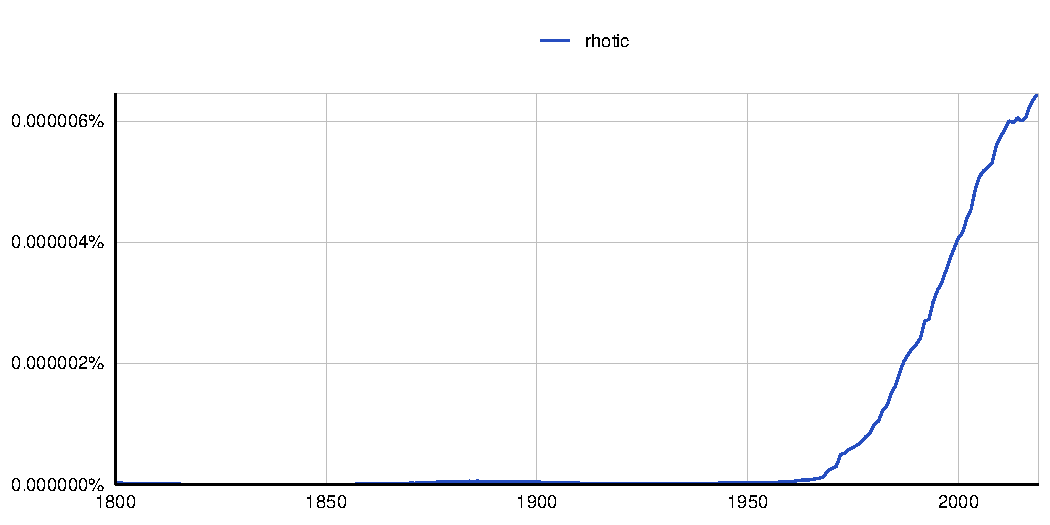
\includegraphics[width=1\linewidth]{images/google_ngram_rhotic}
	\caption[Google n-grams de \textg{rhotic}]{Fréquence de l'expression \textg{rhotic} à partir des données de Google Books en utilisant le package \texttt{ngramr} sur \texttt{RStudio} \parencite{rcoreteamLanguageEnvironmentStatistical2020}, à partir du jeu de données de Google 2019.}
	\label{fig:googlengramrhotic}
\end{figure}

\subsection{Les différents sons \textg{simil-\textit{r}}}

\textcite{wieseRepresentationRhoticsRepresentation2011} établit une liste de huit éléments sur la base des symboles de l'Alphabet Phonétique International qui leurs sont consacrés. Le  r est présent avec le ɾ, le ɹ, le ɺ ou encore le ɽ, le ɻ, le ʀ et le ʁ. Ces segments représentent le cœur des rhotiques et sont généralement présents dans les définitions en extension dans la littérature. À chaque symbole correspond un son et une description articulatoire (que nous appellerons aussi label descriptif dans cette thèse; \textcite{ladefogedSoundsWorldLanguages1996} parlent de définition du segment). \textcite{ladefogedSoundsWorldLanguages1996} dédient un chapitre de leur ouvrage sur les sons du monde aux rhotiques. Dès le début du chapitre, ils se réfèrent aux rhotiques comme une classe de sons comportant entre autres les mêmes huit symboles. On retrouve\footnote{Tous les segments dans la liste sont considérés comme voisés.} :

\begin{enumerate}
	\item Le trill alvéolaire (alveolar trill): r
	\item Le tap ou flap alvéolaire (alveolar tap or flap) : ɾ
	\item L'approximante alvéolaire (alveolar approximant) : ɹ
	\item Le flap alvéolaire latéral (alveolar lateral flap) : ɺ
	\item Le tap ou flap  rétroflexe (Retroflex tap or flap) : ɽ
	\item L'approximante rétroflexe (Retroflex approximant) : ɻ
	\item Le trill uvulaire (Uvular Trill) : ʀ
	\item La fricative uvulaire (Uvular Fricative) : ʁ
\end{enumerate}

Il est possible d'ajouter à ces segments des diacritiques pour spécifier d'autres articulations telles que {\fontspec{Charis SIL}◌̌  } pour les rhotiques fricatives (comme en tchèque), ou {\fontspec{Charis SIL}◌̞} pour les rhotiques approximantes (cf. \autoref{chap:soundcompa} pour un inventaire de diacritiques pouvant être retrouvés avec les rhotiques).\\ 

Nous décrivons brièvement les différents segments sur la base de \textcite{ladefogedSoundsWorldLanguages1996}. Il ne s'agit pas de faire une description complète des rhotiques mais de voir la diversité des articulations qui peuvent être mises en jeu. Le trill, le tap et le flap alvéolaire feront l'objet de sous-sections détaillées.

\subsubsection{Le trill alvéolaire}

Le trill alvéolaire est un son produit lorsque la pointe de la langue entre en vibration avec la crête alvéolaire en raison de conditions aérodynamiques, qui seront détaillées en \autoref{subsec:trill}. Ce trill alvéolaire (que nous appellerons simplement trill dans cette thèse) est représenté par le symbole API [r]. \textcite[218]{ladefogedSoundsWorldLanguages1996} mentionnent que les trills réalisés avec la pointe de la langue ont généralement deux ou trois périodes de vibration. Chaque période est constituée d'une phase ouverte et d'une phase fermée, pendant laquelle les articulateurs sont en contact.

\subsubsection{Les taps ou flaps alvéolaires et rétroflexes}

\textcite[231]{ladefogedSoundsWorldLanguages1996} établissent une distinction précise entre taps et flaps. Le flap implique un mouvement où la langue passe tangentiellement par la crête alvéolaire, alors que le tap implique un mouvement où la pointe de la langue se dirige vers la crête alvéolaire. La section sur les deux segments est relativement courte en comparaison à la présence relativement importante de ces segments dans les langues du monde comme allophones des rhotiques. Pour cela nous développerons d'autres études sur le tap et le flap en \autoref{subsec:acous_tap_flap} pour en comprendre les subtilités articulatoires et acoustiques.


\subsubsection{Les approximantes alvéolaires et rétroflexes}

La description de l'approximante alvéolaire a bénéficié des études portant sur la phonétique et la phonologie de l'anglais puisqu'il s'agit de la rhotique qu'on retrouve en anglais britannique du sud et en anglais états-unien. \textcite{ladefogedPreliminariesLinguisticPhonetics1971} mentionne que l'articulation de l'approximante anglaise peut être alvéolaire ou post-alvéolaire. La pointe de la langue se situe au niveau ou derrière la crête alvéolaire.
En utilisant Uldall (1958)\footnote{Uldall, Elizabeth. 1958. \textg{American \textg{molar} R and \textg{flapped} T.} \textit{Revista do Laboratorio de Fonetica Experimental, Universidad de Coimbra} 4: 103-6.} comme référence, \textcite[234]{ladefogedSoundsWorldLanguages1996} mentionnent qu'il existe aussi une articulation plus complexe, le \textg{bunched r} impliquant deux constrictions : une au niveau du pharynx bas et une au niveau du centre du palais. De plus, cette articulation ne s'accompagne pas d'une élévation de la pointe ou de la lame de la langue. Plusieurs articulations existent pour l'approximante de l'anglais américain bien qu'acoustiquement les segments issus de ces différentes articulations soient similaires.

\subsubsection{Le trill et la fricative uvulaire}

Comme le trill alvéolaire, le trill uvulaire est produit lorsque l'uvule rentre en vibration. 
En se basant sur les travaux de \textcite{delattrePharyngealFeaturesConsonants1971}, \textcite{ladefogedSoundsWorldLanguages1996}, montrent que, de la même manière que les trills alvéolaires, les trills uvulaires varient. Sur la base des travaux de \citeauthor{lindauStory1985}, ils mentionnent que les trills uvulaires intervocaliques sont plus longs que les alvéolaires (p. 226).
Ce son se retrouve en alternance avec la fricative uvulaire, qui est produite lors d'un rapprochement des articulateurs au niveau de la zone uvulaire entraînant de la friction mais sans vibration de l'uvule. Ce son est présent en français \parencite{lancasterBeginningsFrenchUvular1934,hambyePrononciationFrancaisContemporain2005,prematRouleFrancaisDans2018}, en allemand, en néerlandais \parencite{sebregtsSociophoneticsPhonologyDutch2014} et a fait l'objet de recherches en articulation et en acoustique \parencite{gendrotArticulatoryAcousticRealization2016}.

\subsection{Distribution des rhotiques}

Les différents segments n'ont pas la même distribution dans les langues du monde, certains sons étant plus fréquents que d'autres. Avec les données de UPSID, \textcite{maddiesonPatternsSounds1984} montre que, dans son échantillon, plus de 70\% des langues ont au moins une rhotique. Parmi les langues qui ont une rhotique, le trill est présent dans 47,5\% des cas, suivi du tap/flap dans 38,3\% des cas. Les fricatives et approximantes ne représentent que 13,5\%. Cet échantillon de langues permet à \citeauthor{maddiesonPatternsSounds1984} d'affirmer que les sons \textg{simil-\textit{r}} sont généralement voisés, dentaux ou apicaux, et interrompus (il s'agit des trills et des taps/flaps où la langue rentre en contact avec un articulateur fixe, en opposition aux rhotiques continues, plus rares).\\

\subsection{La classe phonologique des rhotiques}

Bien qu'aucune propriété phonétique n'ait été trouvée pour définir en intention ce que sont les rhotiques, de nombreux auteurs/trices se sont penchés du côté du comportement phonologique pour comprendre l'essence même de la classe des rhotiques \parencite{lindauStory1985,dickey1997phonology,magnusonStoryTwoVocal2007,chabotWhatWrongBeing2019}.
Nous reportons ci-dessous deux propriétés mises en avant par \textcite[11]{chabotWhatWrongBeing2019} pour caractériser les rhotiques cross-linguistiquement.

\begin{exe}
	\ex \begin{xlist}
		\ex A rhotic is a segment which may occupy specific syllabic positions—that of the secondary element in branching onsets or codas—and functions as a sonorant regardless of its phonetic instantiation.
		\ex A rhotic demonstrates \textsc{procedural} and \textsc{diachronic stability}: its phonotactic status as a sonorant does not change even when the rhotic is subject to variation due to either diachronic evolution or synchronic processing—for example even if the rhotic is realized as an obstruent.
	\end{xlist}
\end{exe}
\setcounter{exx}{0}

%Le but de cette thèse n'est pas de définir ce qu'est et ce que n'est pas une rhotique mais bien de comprendre que le débat est ouvert et qu'il faut comprendre que la classe des rhotiques existe parce qu'il y a quelque chose dans le comportement de ses membre et dans leurs évolution qui fait qu'ils sont généralement représenté à l'écrit par un <r>.

Le but de cette thèse n'est pas de définir ce qu'est ou n'est pas une rhotique, mais bien de comprendre que ce débat reste ouvert. Cependant, nous gardons en tête qu'au cœur même de l'existence de cette classe des rhotiques se trouvent des caractéristiques spécifiques du comportement de ses membres et de leur évolution qui entraînent leur représentation à l'écrit par un <r>.


%\input{rhotiques/similr}

\section{Aspects de la phonétique et de la phonologie du trill, du tap et du flap}

Avant de commencer à décrire les différents segments d'intérêt, nous devons aborder un point terminologique.
Nous avons fait le choix d'utiliser le terme \textsc{trill}. Nous parlerons de \textg{consonne trillée}, et non de \textg{consonne roulée}. Nous mentionnerons la \textg{consonne trill alvéolaire} et la \textg{consonne roulée alvéolaire}. Nous utiliserons le \textg{phonème trill} et non le \textg{phonème roulée}. Ces emprunts à l'anglais, légèrement francisés, se font au dépit de la terminologie francophone pour deux raisons. Premièrement, la plupart de la littérature existante sur les trills est écrite en anglais. La recherche du terme \textg{alveolar trill} dans les ouvrages scientifiques donne lieu à plus de résultats. Deuxièmement, nos travaux s'inscrivent dans une lignée typologique où la terminologie est cruciale pour mettre en contraste les langues et les comparer. Les descriptions des langues sur lesquelles nous nous appuyons mentionnent plus fréquemment le \textg{trill}, ainsi, il nous apparaît naturel de reprendre le terme le plus commun. De même, nous avons sélectionné les termes de \textsc{tap} et de \textsc{flap}, en dépit de la traduction française \textg{consonne battue}.

\begin{figure}
	\centering
	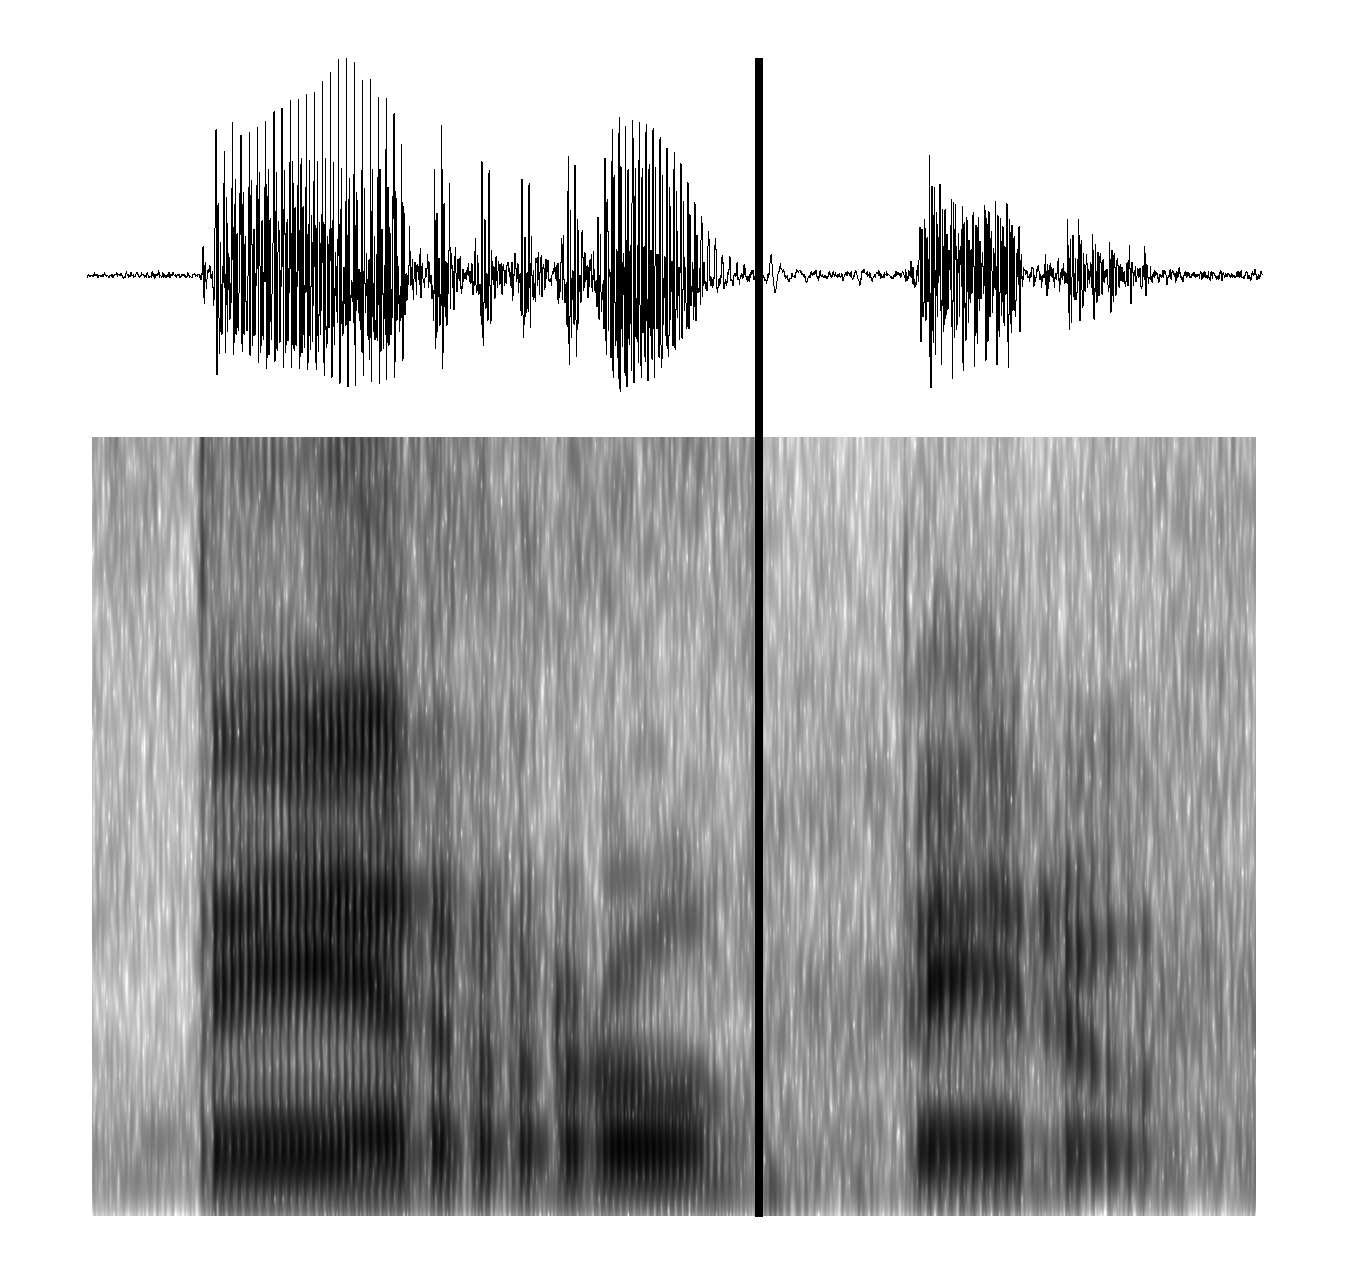
\includegraphics[width=1\linewidth]{rhotiques/images/praat_dogbut.pdf}
	\caption[Illustrations du /r/ et du /ɾ/ en espagnol]{À gauche : le trill dans le mot \textit{perro} /pero/ \textg{chien}. À droite : le tap dans le mot \textit{pero} /ɾ/ \textg{mais}. Les deux exemples sont issus de l'espagnol. Les deux mots ont été produits en isolation, et sont produits par deux locuteurs différents. Le premier (le trill) est produit par un locuteur de 25 ans de Meddelin Antioquia, Colombia, et le second (le tap) par un locuteur de 22 ans de Cartago Valle, Colombia. Le trill et le tap représentés ici sont considérés comme canoniques. L'oscillogramme est donné en haut, et le spectrogramme en bas (les axes sont manquants par choix).}
	\label{fig:praatdogbut}
\end{figure}

\subsection{Description du trill}

Cette sous-section du \textsc{trill} s'intéresse à ce segment d'un point de vue phonétique et phonologique.
Nous reprenons les différentes descriptions de ce segment qui peut impliquer un des trois articulateurs mobiles : les lèvres, la langue, ou l'uvule \parencite{ladefogedLateralsTrills1977}. Il faut souligner que dans cette thèse nous ne nous intéresserons pas aux trills bilabiaux impliquant la vibration des lèvres \parencite{rangelovBilabialTrillsAhamb2019} qui n'ont d'ailleurs jamais été inclus dans la catégorie des rhotiques \parencite{wieseRepresentationRhoticsRepresentation2011}. En ce qui concerne les trills uvulaires, ils sont abordés dans la \autoref{sec:similr} et dans le \autoref{chap:soundcompa}. \\

Nous nous focaliserons uniquement sur la vibration de la pointe de la langue qui donne lieu aux trills apicaux, en laissant de côté celle de la lame de la langue qui donne lieu aux trills laminaux.\\

Contrairement à la sous-section suivante sur le tap/flap, nous ne développerons pas l'origine du terme trill. Cependant, il est important de souligner que le terme peut être ambigu et refléter plusieurs réalités phonétiques de même que le symbole de l'Alphabet Phonétique International \textit{r} (ce point sera développé dans le \autoref{chap:jipa}).

\subsubsection{Acoustique et articulation du trill alvéolaire} \label{subsec:trill}

Le trill alvéolaire apical est un segment produit lorsque la pointe de la langue se maintient de manière lâche près de la crête alvéolaire, de sorte qu'un mouvement d'air fasse vibrer la pointe de la langue. Cela se traduit par des périodes où la langue touche la crête puis s'en sépare \parencite[318]{ladefogedCoursePhonetics2015}.
\textcite[49]{ladefogedLateralsTrills1977} suggèrent que peu de langues possèdent des trills, et que les trills de ces langues sont généralement alvéolaires. Les trills réalisés avec la pointe de la langue ont une fréquence de vibration moyenne de 28,6Hz $\pm$ 4,0.\footnote{\textcite{ladefogedLateralsTrills1977} trouvent que les trills produits avec d'autres articulateurs ont aussi une fréquence de vibration similaire ce qui peut expliquer un degré de similarité auditoire.} \textcite{lindauStory1985} obtient une fréquence de 25Hz sur son échantillon multilingue (soit 1 cycle toutes les 40ms) avec généralement deux à trois périodes. Le nombre de périodes dépend de différents facteurs
\footnote{Certains des facteurs sont développés en \autoref{subsec:trill_tap}.} qui peuvent être linguistiques (le contexte phonologique, la position dans le mot, l'accentuation de la syllabe, le nombre de syllabes du mot, la catégorie grammaticale) \parencite[cf. tableau p. 23 pour les études d'intérêt]{zahlerVariationistAccountTrill2014} et non-linguistiques (le sexe, l'âge [notons que les effets de l'âge et du sexe ne sont pas les mêmes en fonction des études], la classe sociale, le lieu de vie, les croyances, la densité du réseau social des locuteurs, ou encore le style de tâche effectuée pour la récolte de données) \parencite[cf. tableau p. 21-22 pour les études d'intérêt]{zahlerVariationistAccountTrill2014}.\\

Ainsi le trill est souvent caractérisé par la présence d'au moins deux périodes visibles au niveau du signal acoustique (\autoref{fig:praatdogbut}). Chaque période est composée d'une phase de contact (similaire à une obstruction; nous emploierons le terme de \textg{contact} ou d'\textg{obstruction} dans la suite de cette thèse) et une période de relâchement. Le trill à une période reste néanmoins possible, son articulation étant différente du tap/flap \parencite{spajicTrillsToda1996}.

\begin{displayquote}
	\textrm{[...]} even in cases where there is only a single contact with the roof of the mouth, the action is physiologically (but perhaps not auditorily) quite distinct from that of a tap. \parencite[p.50]{ladefogedPreliminariesLinguisticPhonetics1971}
\end{displayquote}


De plus, le trill est caractérisé par des prérequis aérodynamiques fins. \textcite{soleAerodynamicCharacteristicsTrills2002} cherche des tendances universelles dans le comportement des trills. L'autrice montre qu'en cas de manquement des pré-requis aérodynamiques, le segment ne sera pas trillé et/ou dévoisé (le tap est différent de nature et n'a pas de tels prérequis cf. \autoref{subsec:acous_tap_flap}).
En outre, \textcite{mcgowanTongueTipTrills1992} montre que la position de la langue, sa forme et son élasticité, ainsi qu'une différence de pression de part et d'autre de la constriction de la pointe de la langue, jouent un rôle dans l'initiation de la vibration.
\textcite{dhananjayaAcousticAnalysisTrill2012} suggèrent que triller entraîne une géométrie du tract oral qui change rapidement, ce qui rend les trills moins directs à étudier.
Ce sont les différents prérequis du trill qui en font un segment complexe et un des derniers acquis dans les langues du monde \parencite{mcleodChildrenConsonantAcquisition2018}.\\

Il n'existe pas à notre connaissance d'autres études sur la perception du trill, et de la discrimination de contraste de longueur, au sein d'une même langue autre que celle de \textcite{raymondInitialMedialGeminate2005}. Cette étude sur l'arop-lopek \glotto{arop1243}, langue parlée en Papouasie-Nouvelle-Guinée par quelques 3000 locuteurs/trices, s'intéresse au contraste entre le /r/ et le /rr/, la contrepartie géminée du /r/. Le flap [ɾ] est aussi présent dans la langue comme allophone intervocalique du /d/.
Trois études sont incluses dans l'article.
La première étude se focalise sur la production des trills et s'intéresse au nombre minimum, moyen et maximum de contacts que les trills et les trills géminées peuvent avoir.
La deuxième étude cherche à savoir si les locuteurs sont capables de discriminer, faire la différence entre un trill géminé et un trill non géminé. 
Finalement, la dernière étude se concentre sur la compréhension de la frontière de perception entre un trill et un trill géminé.\\

\textcite{raymondInitialMedialGeminate2005} ont enregistré six locuteurs mâles pour leur étude de production lors d'une tâche de lecture de liste de mots. Les trills en position intervocalique et finale pouvaient avoir au minimum un contact (88/364) ce qui n'était pas le cas lorsqu'ils étaient en position initiale (0/131). Certains trills géminés étaient aussi produits avec un contact, bien que ce n'était pas les productions les plus fréquentes (5 occurrences sur 218). Les trills en position initiale sont plus longs que les trills dans les autres positions.
Les trills ont été produits avec maximum 5 contacts, alors que les trills géminés ont été produits avec maximum 7 contacts.
Les trills géminés sont produits avec plus de contacts (en moyenne 3,76 contacts) que les trills non géminés (en moyenne 2,29 contacts).
L'étude de discrimination sur le terrain a permis de mettre en avant que les locuteurs sont capables de discriminer correctement un trill d'un trill géminé en position initiale et intervocalique. L'étude de perception sert à montrer qu'à partir de trills modifiés artificiellement, les locuteurs catégorisent dans les trills, les items avec moins de contacts, et dans les trills géminés, ceux avec le plus de contacts. De même que pour l'étude en production, une asymétrie existe entre les items en position initiale et ceux en position intervocalique. En position initiale, il faut plus de contacts pour qu'un item soit considéré comme un trill géminé.\\

La position en début de mot est favorable aux trills. Cependant, les rhotiques ont tendance a être défavorisées en initiale de mot à travers les langues \parencite{labruneWordinitialRhoticAvoidance2021}. Ces résultats sont néanmoins à mettre en contraste avec \textcite{kavitskayaTrillsPalatalizationConsequences2009} qui, sur la base de données du russe, montrent que le trill est défavorisé en position intervocalique. Cela permettrait d'expliquer les distributions des différents allophones des rhotiques cross-linguistiquement.\\


Les trills sont souvent étudiés par rapport à des langues indo-européennes, à l'exception de quelques études typologiques.
L'étude de \textcite{raymondInitialMedialGeminate2005} est intéressante car elle apporte de la phonologie de laboratoire sur le terrain avec une expérience de production, de discrimination et de perception. De plus, elle s'intéresse à une langue sous-étudiée (sur \href{https://www.google.com/maps/place/Matafum,+Papouasie-Nouvelle-Guin\%C3\%A9e/@-5.2182111,146.4002482,9.13z/data=!4m13!1m7!3m6!1s0x68f3e3520a551b3f:0x58a83294038393a4!2sLong+Island!3b1!8m2!3d-5.3535839!4d147.1464245!3m4!1s0x68f3fd93309894d3:0x2df33848a2f3c3c0!8m2!3d-5.3707325!4d147.0343745}{Long Island} en Papouasie-Nouvelle-Guinée) dans une aire géographique et dans une famille linguistique (austronésienne) et permet d'apporter des éléments de réflexion sur le contraste que peuvent faire les langues entre trois sons \textg{simil-r} : le flap, le trill et le trill géminé.


\subsection{Description du tap et du flap}

Après avoir décrit les principales caractéristiques du trill, nous décrivons le tap et le flap. Nous avons pris le soin de développer cette sous-section sur le tap et le flap car \textg{
[t]he alveolar tap is a fairly understudied rhotic, and many aspects of its variation within and between speakers as well as across languages are not fully known \parencite[86]{cathcartArticulatoryVariationAlveolar2012}}. Tout d'abord nous aborderons l'historique des termes tap et flap avant de décrire articulatoirement et acoustiquement ces segments.

\subsubsection{Terminologie et historique du tap/flap}

\begin{figure}
	\centering
	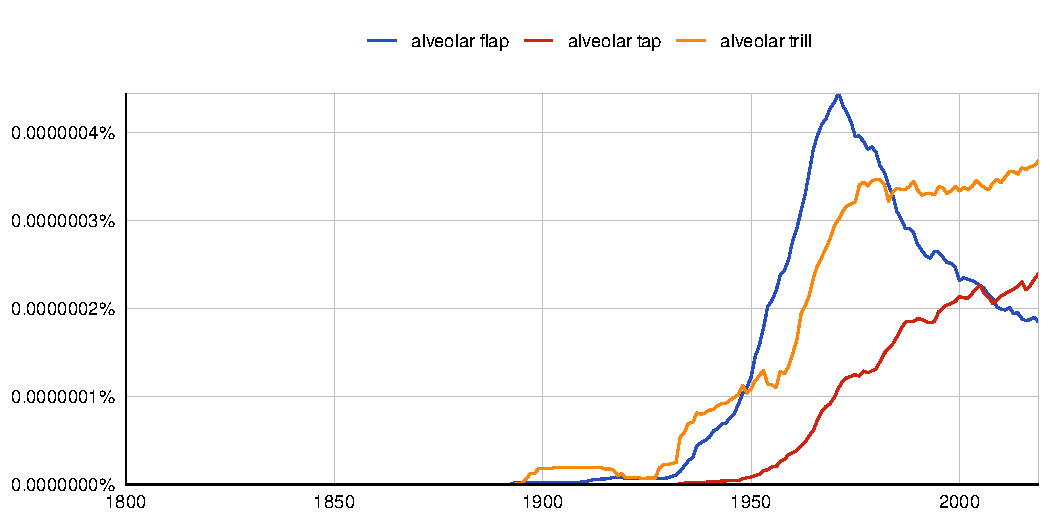
\includegraphics[width=1\linewidth]{images/google_ngram_trill_tap_flap}
	\caption[Google n-grams de \textg{alveolar trill}, \textg{alveolar tap}, \textg{alveolar flap}]{Fréquence des expressions \textg{alveolar trill}, \textg{alveolar tap}, \textg{alveolar flap} à partir des données de Google Books en utilisant le package \texttt{ngramr} sur \texttt{RStudio} \parencite{rcoreteamLanguageEnvironmentStatistical2020}, à partir du jeu de données de Google 2019.}
	\label{fig:googlengramtrilltapflap}
\end{figure}


On retrouve deux grandes approches concernant les taps et flaps. D'un côté, les études qui s'intéressent aux segments en prenant comme langue de référence l'anglais parlé aux États-Unis où le [ɾ] est un allophones des obstruentes /t, d/. De l'autre côté, il s'agit des études qui opposent le tap et le flap au trill car dans les langues étudiées on retrouve deux phonèmes /ɾ/ et /r/ comme en catalan. Il existe aussi une littérature moins abondante qui s'intéresse aux taps et flaps avec un point de vue utilisant d'autres langues.\\

Le \textg{trill} est apparu en premier, suivi du \textg{flap} puis du \textg{tap}. De la même manière, le symbole \textit{r} est apparu avant le \textit{ɾ} dans l'Alphabet Phonétique International. Nous avons fait le choix de garder le terme tap dans cette thèse comme terme générique pour parler des taps et des flaps. Nous justifions ce choix par l'éducation linguistique que nous avons reçue où le terme \textg{tap} était plus fréquent que le terme \textg{flap} reflétant leurs usages dans les publications scientifiques (Figure \ref{fig:googlengramtrilltapflap}). Le terme de flap est vraisemblablement d'abord apparu sur le continent européen où on le retrouve rapidement dans les publications de \textit{Le maître phonétique}. L'espagnol y était décrit avec un flap \parencite[8]{passySupplementAimPrincipales1904} et un trill. Le terme de tap, lui, est sûrement apparu sur le continent américain pour faire spécifiquement référence à l'allophone battu du /t/ et du /d/ produit en anglais américain entre deux voyelles. On retrouve dès les années 40 avec John Samuel Kenyon et Kenneth L. Pike l'apparition du terme \textg{tap}.

\begin{displayquote}
Voiced \textbf{t} is often described as a single-tap \textbf{r}. To the author's ear the two are quite distinct. Even when the voiced \textbf{t} has repeated taps (trilled  \textbf{t}) it is acoustically distinct from trilled \textbf{r} [...] \parencite[127]{kenyonAmericanPronunciation1943}
\end{displayquote}


\begin{displayquote}
In \textit{flap articulation} the articulator gives one rapid tap against its articulating region and then immediately releases; approach and release together are formed by a single ballistic movement. \parencite[124-125]{pikePhoneticsCriticalAnalysis1943}\
\end{displayquote}

En 1964, \citeauthor{ladefogedPhoneticStudyWest1968}\footnote{Nous n'avons pu consulter que la version de 1968.} publie un ouvrage sur les langues d'Afrique de l'ouest dans lequel il met en évidence que le hausa \glotto{haus1257} contraste entre un tap, qui peut être réalisé comme un trill, et un flap. Il s'agit de la première occurrence que nous avons trouvée où le tap est explicitement opposé au flap. Ses travaux lui permettront en \citeyear{ladefogedPreliminariesLinguisticPhonetics1971} de définir le tap comme un son où \textg{[o]ne articulator [is] thrown against another} et le flap comme un son où \textg{[o]ne articulator striking another one is passing} \parencite[46]{ladefogedPreliminariesLinguisticPhonetics1971}. Ces descriptions vont évoluer au fil des recherches menées sur les deux sons avec une influence sur le reste de la linguistique descriptive de terrain (comme nous le verrons avec les différences de terminologie dans le \autoref{chap:metagram}).

\begin{displayquote}
Alveolar tap ɾ also occurs in Hausa. Most of my informants used this sound, although occasionally it was replaced by a trilled r. Both these sounds occurred where Hausa orthography has r. There is also a contrasting sound which is sometimes written as r, and which appears to be a retroflex flap ɽ. [...] The nearest I can come to agreeing with this is to say that the first sound is a trill which has a statistical probability of consisting of only one tap. \parencite[30]{ladefogedPhoneticStudyWest1968}
\end{displayquote}

Cette section a servi à mettre en évidence que l'existence des deux termes tap et flap est historiquement justifiée. Les publications contemporaines font souvent le choix d'un terme ou de l'autre (ce qui n'est pas problématique, cela n'ayant pas de conséquences pour les analyses).\footnote{Par exemple, dans notre \autoref{chap:jipa} sur les \textit{Illustrations of the IPA} nous avait fait le choix (qui n'était pas vraiment éclairé au moment de l'écriture) d'utiliser le terme \textg{tap}.}

\subsection{Acoustique et articulation du tap/flap} \label{subsec:acous_tap_flap}

Nous détaillons dans cette sous-partie les différentes études qui ont eu comme objet de recherche le tap et/ou le flap.
\textcite[128]{catfordFundamentalProblemsPhonetics1977}, se basant sur les travaux de \textcite{ladefogedPhoneticStudyWest1968}, utilise le terme \textg{flap}. Le flap est articulatoirement décrit comme un son produit lorsqu'un organe articulatoire approche un autre (stationnaire) créant un contact momentané avant de se retirer (aussi connu sous le nom de \textg{one-tap r}). Deux types de flaps sont mis en avant en fonction de la mise en action de la langue. D'un côté, les flaps \textg{flick} [ɾ] sont produits lorsque l'articulateur revient à sa position de départ, et de l'autre, les flaps \textg{transient} [ɽ] sont produits lorsque l'articulateur mobile entre en contact momentané avec l'articulateur fixe dans son mouvement vers une position finale (Figure \ref{fig:figure29catford}). Les deux types de segments ont une durée comprise entre 10 et 30ms.\\

\begin{figure}
	\centering
	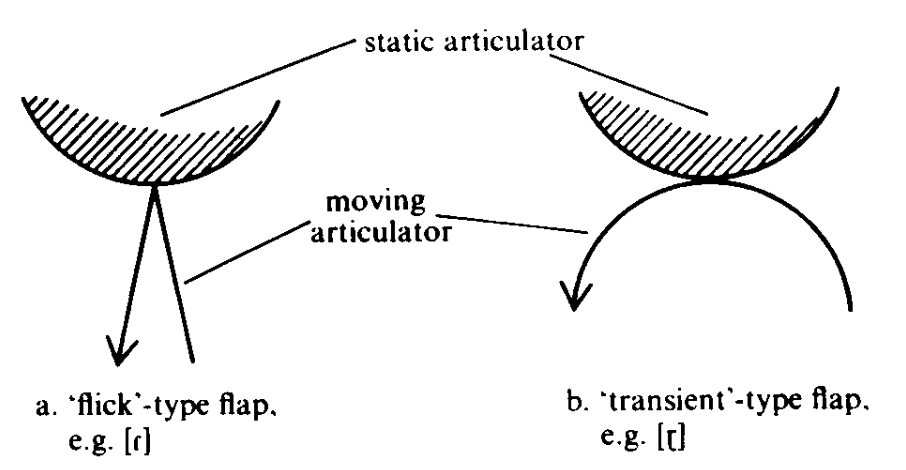
\includegraphics[width=0.9\linewidth]{rhotiques/images/figure_29_catford}
	\caption[Schématisation des \textg{flaps}. Figure issue de Catford (1977)]{Schématisation par \textcite[129]{catfordFundamentalProblemsPhonetics1977} des deux types de flaps identifiés. L'un sera généralement repris par la littérature comme un tap [ɾ], et l'autre comme un flap [ɽ].}
	\label{fig:figure29catford}
\end{figure}

\textcite[129]{catfordFundamentalProblemsPhonetics1977} souligne l'importance de la momentanéité des flaps, des mouvements balistiques, les opposant aux stops : \textg{a stop can be prolonged; a flap cannot be prolonged}.\footnote{\textcite[397]{newmanHausaLanguageEncyclopedic2000} mentionne qu'en hausa le flap géminé existe de même que le \textg{tap/roll} geminé. Le flap géminé se manifeste phonétiquement par une augmentation de la \textg{temporal period of the retroflex flap gesture}, là où le \textg{tap/roll} devient un trill discernable. \textcite[237]{ladefogedSoundsWorldLanguages1996}, en hausa, analysent la géminée du flap comme une longue approximante rétroflexe.} Contrairement aux stops, les flaps mettent en jeu une surface de contact moins importante selon \textcite[251]{catfordFundamentalProblemsPhonetics1977}.\\

En anglais américain, le flap peut être un allophone du /t/ et du /d/. Le flap est un des allophones des occlusives alvéolaires en position post-voyelle accentuée \parencite{zueAcousticStudyMedial1979}.
Avec des enregistrements de trois hommes et trois femmes, les auteurs analysent les données et soulignent la présence de variation dans les réalisations des flaps. En effet, la phase de \textg{closure} peut être plus ou moins complète. Lorsqu'elle est partielle, on peut retrouver au niveau du signal acoustique de la turbulence similaire à celle qu'on peut retrouver avec les fricatives voisées. Les auteurs mesurent en moyenne 27 ms pour les /d/ et 26 ms pour les /t/ avec un écart autour de la moyenne entre 10 ms et 40 ms, principalement dû au contexte vocalique. Une durée courte de flap indique un mouvement rapide de la langue montant et descendant de la pointe de la langue, alors qu'une durée longue est indicatrice d'une pression accumulée pendant la constriction de la langue qui s'accompagne d'un relâchement accompagné par une explosion de bruit visible sur le spectrogramme. Cela peut s'expliquer par la position du corps de la langue. S'il est bas, alors le mouvement de la pointe de la langue peut être bref, alors que s'il est haut, le mouvement de la pointe de la langue \textg{overshoot} la zone alvéolaire rendant l'occlusion plus longue.\\


\textcite{zengUnderstandingFlappingXiangxiang2007} s'intéresse aux flaps dans le dialecte chinois de Xiangxiang\footnote{Selon nous, il est regrettable que cette description allophonique ne soit pas présente dans l'\textit{Illustration of the IPA} publiée, disponible en FirstView (cf. \autoref{subsec:data_coll}) à propos du même dialecte du chinois \parencite{zengXiangxiangDialectChinese2020}. Nous nous interrogeons donc sur la proportion des langues décrites dans JIPA à avoir des occlusives qui sont réalisées comme des flaps dans certains contextes, mais qui ne sont pas décrites comme telles.} qui sont des allophones du /d/ et du /t$^\textrm{\tiny h}$/ en position intervocalique pré-syllabe accentuée et pré-syllabe non accentuée. L'étude se base sur quatre locuteurs et une locutrice et permet de mettre en évidence de la variation intra-individuelle. \citeauthor{zengUnderstandingFlappingXiangxiang2007} montre qu'il existe dans cette position pour le /d/ un continuum allant du [d] \textg{typique}, avec une occlusion longue et une barre d'explosion, au flap, avec une occlusion de courte durée et sans barre d'explosion. Dans ce continuum, on retrouve aussi le flap long avec une durée plus longue que le flap typique, et le [d] court avec une durée d'occlusion plus courte que celle du [d] typique.
Un dernier variant, considéré comme \textg{extrême} par \citeauthor{zengUnderstandingFlappingXiangxiang2007}, possède une structure similaire à celle d'une approximante, c'est-à-dire avec un degré moindre de constriction orale. Pour le /t$^\textrm{\tiny h}$/, cinq variants sont identifiés :

\begin{itemize}
\item le typique [t$^\textrm{\tiny h}$],
\item le typique [d$^\textrm{\tiny h}$],
\item le court [d$^\textrm{\tiny h}$],
\item le flap aspiré long
\item et le flap aspiré typique.
\end{itemize} 

Des données aérodynamiques sont aussi incluses et permettent de montrer une relation entre le flux d'air oral et les différents motifs acoustiques.
Ainsi, \textcite{zengUnderstandingFlappingXiangxiang2007} montre que le processus de \textg{flapping} n'est pas binaire. L'accentuation de la voyelle précédente est exclue comme facteur explicatif des différents variants mais les voyelles précédentes et suivantes permettent d'expliquer la variation à cause de co-articulation.\\

\textcite{sonPitfallsSpectrogramReadings2008}, dans la continuité de \textcite{zengUnderstandingFlappingXiangxiang2007}, s'intéresse au flap allophone de la liquide /l/ en coréen. Son étude inclut des données acoustiques de deux locutrices native de Séoul en plus de mesures articulométriques. \citeauthor{sonPitfallsSpectrogramReadings2008} met en évidence de la variation intra-individuelle avec cinq variants :

\begin{itemize}
	\item Flap voisé avec explosion
	\item Flap voisé sans explosion
	\item Flap partiellement voisé avec explosion
	\item Flap non voisé avec explosion
	\item Flap \textg{extrême} (reprenant la description de \textcite{zengUnderstandingFlappingXiangxiang2007})
\end{itemize}

L'étude articulatoire a permis de montrer que, même lorsqu'il n'y avait pas de constriction dans le cas des flaps extrêmes, il y avait quand même un mouvement large de la pointe de la langue, mettant en évidence une certaine invariance dans l'articulation du flap. Cette invariance est donc à mettre en contraste avec la variation dans les résultats des études acoustiques.\\

Les travaux initiés par Derrick, Gick et leurs collègues \parencite{derrickQuantitativeAnalysisSubphonemic2008,derrickTwoPhonologicalSegments2010,derrickIndividualVariationEnglish2011,derrickAcousticCorrelatesFlaps2013} sur la base d'ultrasons ont permis de mettre en avant la variation dans les mouvement associés au processus de \textg{flapping} en anglais américain. On retrouve quatre variants (Figure \ref{fig:tapflap}):

\begin{itemize}
	\item Up-flap
	\item Down-flap
	\item Alveolar tap - le tap alvéolaire
	\item Postalveolar tap - le tap post-alvéolaire
\end{itemize} 

La catégorisation des différents variants s'est faite en fonction du mouvement de la pointe de la langue, ainsi que de sa direction. Les travaux préliminaires de \textcite{derrickQuantitativeAnalysisSubphonemic2008} montrent que tous les participants produisent les quatre variants et que la variation est influencée par la position de la langue avant et après le segment \parencite{derrickTwoPhonologicalSegments2010}. \textcite{derrickIndividualVariationEnglish2011}, en étudiant huit locutrices et dix locuteurs, obtiennent que trois participants n'ont pas produit un des variants (le tap post-alvéolaire). Ainsi, les auteurs montrent que les réalisations \textg{flap} sont plus fréquentes que les réalisations \textg{tap}. On retrouve en plus de la variation non-conditionnée puisque pour les mêmes mots, certains participants ont utilisé différentes stratégies articulatoires. \\

\begin{figure}
	\centering
	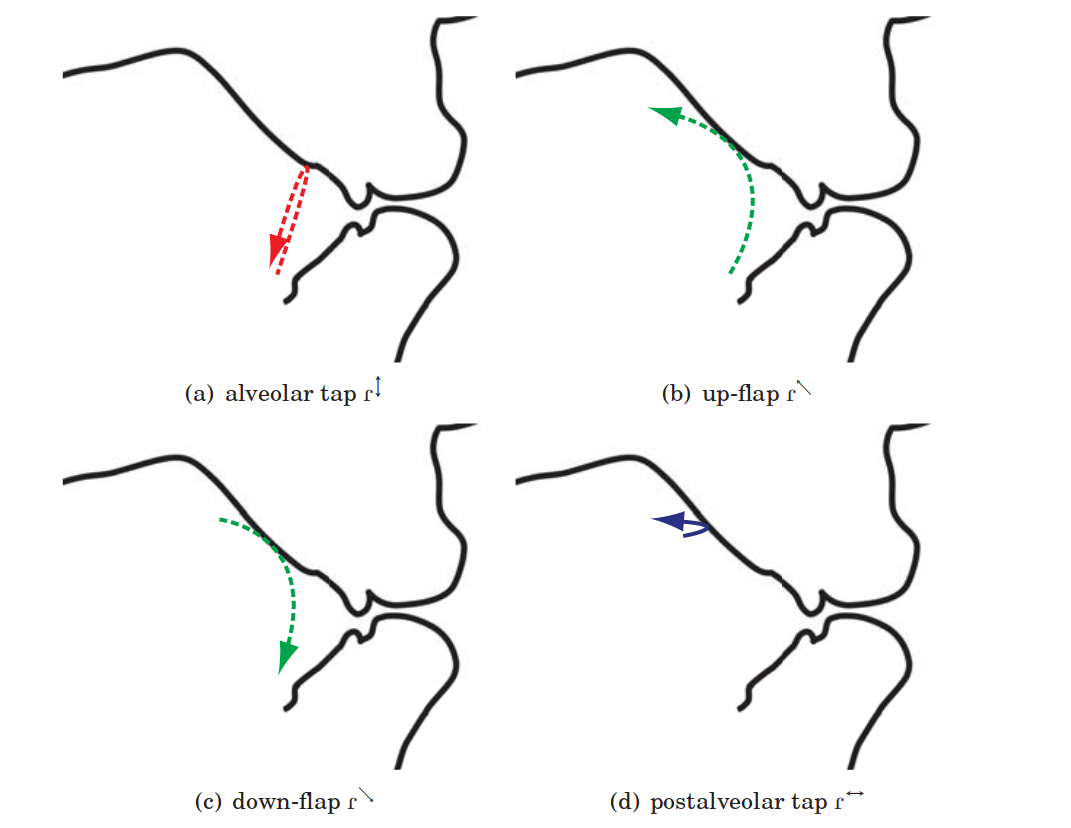
\includegraphics[width=0.7\linewidth]{rhotiques/images/tap_flap}
	\caption[Différents mouvements pour le tap/flap en anglais américain. Figure issue de \textcite{derrickAcousticCorrelatesFlaps2013}]{Les différents mouvements pour le tap/flap en anglais américain. La figure est issue de \textcite{derrickAcousticCorrelatesFlaps2013}. Les différents mouvements ont été obtenus par ultrason.}
	\label{fig:tapflap}
\end{figure}

\textcite{derrickIndividualVariationEnglish2011} offrent un nouveau regard sur les données de différentes langues. Pour eux, les contrastes entre les quatre différents variants du flap sont possibles. Ils mettent en avant des contrastes phonétiques sur la base de contrastes entre tap et flap, comme c'est le cas pour le punjabi\footnote{Il existe une \textit{Illustration of the IPA} pour le punjabi \parencite{hussainPunjabiLyallpuriVariety2019} où les auteurs mentionnent un contraste entre deux rhotiques : un tap alvéolaire /ɾ/ et un tap rétroflexe /ɽ/ (\textg{retroflex tap} [\textit{sic}] (p. 6). Les auteurs illustrent une paire minimale et explicitent que la consonne rétroflexe met en avant un abaissement précoce des troisième et quatrième formants.} \parencite[645]{shacklePanjabi2003}, ou le norvégien où l'on retrouve un [ɾ] s'opposant à un [ɽ] dans certains dialectes \parencite[24]{kristoffersenPhonologyNorwegian2000}.\\

L'étude préliminaire de 2013 de \citeauthor{derrickAcousticCorrelatesFlaps2013} s'intéresse à l'acoustique des quatre variants. Les auteurs montrent qu'il y a des différences significatives pour la fréquence fondamentale et les cinq premiers formants entre les variants. Des deux premiers formants, les auteurs concluent que les quatre variants ont des configurations différentes en termes d'aperture et de postériorité, mais que ces différences se réduisent après la consonne. En ce qui concerne le troisième formant, les auteurs concluent que les variants ont différents points de contact. Le down flap a son point de contact le plus proche des dents, suivi du tap alvéolaire et du up flap, et c'est le tap post-alvéolaire qui a son point de contact le plus haut.\\

Dans certains cas, le tap/flap n'est pas considéré comme un allophone d'un stop mais d'une rhotique, c'est le cas de l'espagnol ou du catalan où le tap a été étudié en opposition à une autre rhotique de ces langues : le trill. Nous avons détaillé les études sur le trill en \autoref{subsec:trill} et nous faisons le lien entre les deux segments en \autoref{subsec:trill_tap}. Dans cette section, nous ne parlerons que du tap/flap.

\textcite{recasensProductionCharacteristicsApicoalveolar1991} étudie de manière préliminaire les caractéristiques de production du tap apico-alvéolaire en catalan avec l'électropalatographie sur la base de ses propres productions.
L'occlusion n'est pas systématiquement complète pour le tap. Il y a plus de contact pour le tap lorsqu'il est précédé et suivi par une voyelle postérieure [a, u] que lorsqu'il est précédé et suivi par une voyelle antérieure [i]. Ce manque de contact associé à la voyelle antérieure [i] suggère, selon \citeauthor{recasensProductionCharacteristicsApicoalveolar1991}, qu'il peut exister une incompatibilité entre la constriction de la pointe de la langue et l'élévation du dos de la langue. Ses résultats lui permettent aussi de supposer que la position du corps de la langue ne nécessite pas tant de contrôle articulatoire, à cause de la présence de coarticulation avec le contexte vocalique. L'étude de \textcite{recasensStudyLightDAC1999}, avec plus de participants, vient confirmer les résultats de l'étude préliminaire. Les deux études mettent principalement en avant les différences en terme de coarticulation entre le trill et le tap plutôt que de caractériser finement le tap.

\begin{displayquote}
	The tap is articulated with a restricted short apicoalveolar closure and more predorsum lowering than other alveolars. In comparison with /n/, /ɾ/ involves less apico-predorsal coupling and exhibits larger dorsopalatal and F2 troughs in the sequence /iCi/. \parencite[163]{recasensStudyLightDAC1999}
\end{displayquote}

Des études dans d'autres langues soutiennent également l'appartenance du tap et du flap dans la catégorie des rhotiques. Par exemple, \textcite[96]{carvalhoEstruturasFoneticasLingua2010} effectue une analyse acoustique préliminaire du flap en tikuna où il est considéré comme une rhotique. \citeauthor{carvalhoEstruturasFoneticasLingua2010} obtient de la variation inter-individuelle  mais aussi intra-individuelle avec un continuum allant de l'occlusion brève mais complète à l'approximante. Des quatre locuteurs enregistrés, un a présenté des occurrences avec systématiquement une constriction, un a systématiquement produit des flaps sans constriction, et deux ont produit un mélange des différents variants. Toutes les productions de flaps étaient voisées et avaient une durée moyenne de 21 ms. \textcite{savuMoreRhoticTap2014} s'intéresse au tap en macédonien et en roumain en mettant en évidence les différences de perceptions entre les locuteurs des deux langues.\\

Pour étudier la rhotique du grec, \textcite{baltazaniManyFaces2013} combinent une étude articulatoire et acoustique. La rhotique a été généralement décrite comme un tap en position intervocalique. Les résultats de l'étude confirme que la rhotique est très majoritairement produite avec un contact court dont la durée varie entre 11 et 57 ms, ce que les auteurs interprètent comme un tap. Des trills sont aussi retrouvés parmi les productions. Le degré de constriction est variable car influencé par plusieurs facteurs. Des différentes expériences menées, plus de 50\% des occurrences sont produites avec une constriction incomplète. Ce contact incomplet se retrouve notamment lorsque les taps ne sont pas produits dans un groupe consonantique. De même, le contact incomplet se retrouve plus dans les syllabes hétérosyllabiques ainsi qu'en position initiale de mot ou lorsque le segment est adjacent à une fricative (en opposition à un stop). De plus, les auteurs mettent en avant l'importance d'un élément vocalique pour le mouvement du tap.

%Parmi les éléments acoustiques qui caractérisent le rabat en tant que "segment acoustique" (cf. Fant 1973 ; Recasens 1991b ; Ting 2007 ; Son 2008) figurent les suivants :
%(1) durée de la discontinuité spectrographique introduite par le geste d'occlusion ;
%(2) l'intensité de la discontinuité (caractérisant une occlusion complète ou une zone plus large au point de contrition) ;
%(3) le modèle de transition des formants dans les voyelles voisines ;
%(4) présence ou absence de voisement ;
%(5) présence ou absence de formants pendant la discontinuité ou l'occlusion.






\section{Distribution et variation cross-linguistique des sons \textg{simil-\textit{r}}}

\subsection{Distribution dans le monde}

Deux travaux d'importance ont eu comme objectif d'étudier la variation dans les trills avec une approche typologique (avec un recours minimal à des bases de données existantes). Paradoxalement, bien que le thème de ces travaux soit directement relié au contenu de cette thèse, nous n'avons pas eu d'accès direct aux ouvrages à l'exception de \textcite{lindauStory1985}.
Nous allons tout d'abord détailler le manuscript non publié de Jones\footnote{Jones, M. (unpublished). Patterns of variability in apical trills: An acoustic study of data from 19 languages.} puis la thèse de \textcite{inouyeTrillsTapsStops1995} et finalement les travaux de \textcite{lindauStory1985}.\\

Pour cela, nous avons fait le choix de rapporter ces travaux à travers leurs citations dans la littérature. Comme il s'agit de travaux qui étudient plusieurs langues en même temps, nous pouvons supposer que la même méthodologie a été utilisée pour étudier les langues, et donc dans une certaine mesure contrôler la variation entre les productions.\\

\textcite[23]{punnooseAuditoryAcousticStudy2010} mentionne que Jones considère le trill comme central dans les rhotiques, bien que cela puisse amener à l'interprétation fausse qu'une langue avec un /r/ trillé le réalise forcément comme un trill [r]. Jones met en avant de la variabilité dans son étude sur 19 langues due à la complexité articulatoire du segment\footnote{Les différents aspects qui font du trill un segment complexe sont abordés en \autoref{subsec:trill} et dans le \autoref{chap:jipa}}. Les 19 langues utilisées possèdent une seule rhotique. Jones s'intéresse aux rhotiques dans des listes de mots mais aussi dans des histoires \textg{narratives} récoltées en laboratoire. Ses résultats (p. 23 dans \textcite{punnooseAuditoryAcousticStudy2010}) montrent que le trill n'est réalisé comme tel que dans un tiers des cas avec généralement deux occlusions. Les trills sont moins fréquents dans les narratives que dans les listes de mots, et également plus fréquents dans des contextes consonantiques qu'en position intervocalique avec le contexte post-vocalique pré-consonantique favorisé.
Acoustiquement, \textcite[24]{punnooseAuditoryAcousticStudy2010} explique les résultats de Jones par la présence d'un deuxième contact des trills, généralement affaibli. Cela peut se traduire par un manque de détection de la part d'études acoustiques. Enfin, cela donne du crédit à l'hypothèse que ce genre de trill cause une réanalyse perceptuelle menant à un changement du trill au tap. Cependant, pour Jones il existe aussi des réalisations non trillées qui sont des taps. Il ne peut pas affirmer que ces taps soient qualitativement différents des \textg{one-contact trill} (p. 24).\\

Du résumé de la thèse de \textcite{inouyeTrillsTapsStops1995}, nous pouvons dire que l'autrice s'est intéressée à la relation entre trills, taps et stops. L'originalité de sa thèse est d'avoir travaillé sur quelques 65 familles de langues, et d'y avoir inclus des données phonétiques d'environ une quinzaine de langues. Ces données sont des données de première main mais aussi de bases de données déjà existantes (au moins pour les langues australiennes incluses et celles provenant de UCLA phonetic database). L'autrice montre dans sa thèse que les taps comme allophones intervocaliques d'occlusives sont fréquents dans les langues du monde, de même que l'allophone tap en position intervocalique dans les langues décrites avec un trill.\\

\textit{The Story of /r/} de \textcite{lindauStory1985} cherche ce qui caractérise les rhotiques. Pour ce faire, sans détailler sa méthodologie, l'autrice utilise les productions de 92 locuteurs/trices issus de plus de 13 langues/dialectes dont 9 avec un trill [r] comme allophone. Ses données lui permettent de comparer les trills alvéolaires et les trills uvulaires  et d'en dégager les tendances acoustiques. Ses mesures du troisième pic spectal (le troisième formant F3) suggèrent que les productions des trills sont variables chez des locuteurs/trices qui produisent des segments avec un lieu d'articulation plus ou moins alvéolaire, ou plus ou moins dental (de même \textcite{dhananjayaAcousticAnalysisTrill2012} montrent que les trills sont flexibles quant à la position du dos de la langue). La contribution la plus importante de \citeauthor{lindauStory1985} utile à notre thèse est d'affirmer que la réalisation du /r/ comme consonne trillée n'est pas commune même lorsque ces sons ont été décrits comme étant des \textg{trills} (p. 161). En effet, d'autres réalisations sont possibles comme des taps ou des approximantes. \citeauthor{lindauStory1985} met ainsi en avant de la variation à la fois entre les individus (variation inter-individuelle) et au sein des productions des mêmes individus (variation intra-individuelle), qui ne sont pas toutes trillées (sauf pour l'espagnol\footnote{Bien que peu d'occurences de trills en espagnol sont incluses dans notre analyse acoustique, nous retrouvons aussi cette tendance dans le \autoref{chap:acoustics}}).\\
	

\subsection{Exemples de la variation en français et en espagnol autour du monde}

Nous montrons que la variation n'est pas seulement inter-langues mais peut aussi se retrouver au sein de langues parlées à plusieurs endroits du globe avec un héritage colonial. C'est le cas du français et de l'espagnol que nous illustrons dans les sous-sections suivantes.

\subsubsection{Les productions du /r/ dans la francophonie}

Le /r/ français n'est pas uniquement articulé comme une fricative ou une approximante alvéolaire. Ainsi, dans certaines régions du monde francophone il est encore possible de trouver des réalisations de la rhotique alvéolaire. En ce qui concerne les productions uvulaires, elles sont, de même que pour les rhotiques alvéolaires, maîtrisées tardivement par les enfants \parencite{dossantosDeveloppementPhonologiqueFrancais2007,metralCaracterisationAcoustiqueRhotique2021}.\\

Le français s'est exporté dans différentes régions du monde, entraînant des changements spécifiques à chaque région où il a été nouvellement parlé. De manière générale, on retrouve une tendance pour la rhotique apicale à laisser place à la rhotique uvulaire. \textcite{thibaultFrenchOutsideEurope2022} nous résume les différentes études mettant en évidence les variations dans les sons du français en fonction des différentes ères coloniales. Nous présentons les aires géographiques avec les différentes réalisations dans l'ordre donné par \citeauthor{thibaultFrenchOutsideEurope2022}. La variation n'est pas détaillée, avec dans la plupart des cas un ou deux allophones majoritaires décrits à travers leur symbole de l'API.\\

Le français de Saint-Laurent utilise un [r] apical qui est en cours de changement en faveur du [ʁ] uvulaire, de même qu'en français de Montréal \parencite{sankoffInstabilityAlternationMontreal2013,morinApicalUvularWhat2013}.
Le français acadien utilise le flap [ɾ]. Similairement, on retrouve le flap [ɾ] dans le français de Louisiane. À Haïti, en Guadeloupe ou en Martinique, on retrouve différents allophones dont les fricatives [ɣ] vélaire et [ʁ] uvulaire ainsi que l'approximante [w].
Dans les îles de l'océan Indien, en Mauritanie le /r/ est soit supprimé, soit produit uvulairement avec peu d'intensité \parencite[263--264]{ledegenFrenchMauritiusSpeaker2016}.
Au Maghreb, la rhotique a été produite comme un trill alvéolaire [r] mais un changement est en cours et elle est principalement produite comme le [ʁ] uvulaire\footnote{\textcite{thibaultFrenchOutsideEurope2022} référant à Morsly (2003, p. 937) ne mentionne que les productions des hommes sans expliciter ce que les femmes produisent.} Ce changement de la production alvéolaire à l'uvulaire est aussi présent au Liban où les locuteurs jeunes et cultivés préfèrent le [ʁ] uvulaire parisien \parencite[25]{thibaultFrenchOutsideEurope2022}. En Afrique subsaharienne, on retrouve le [r]. 
Dans le français du Djibouti, le flap [ɾ] est présent, dans celui de Madagascar, il s'agit d'un trill [r]\footnote{De même que pour le /r/ du Maghreb, \textcite{thibaultFrenchOutsideEurope2022} réfère à Bavoux (1993, pp. 181-183) pour insister sur le fait que la variante est principalement présente chez les hommes.}. 
Finalement, dans le Pacifique, à Tahiti, le /r/ est réalisé comme un flap alvéolaire ou trill [r].

\subsubsection{Les productions du /r/ dans le monde hispanique}

De même que le français, l'espagnol s'est exporté à l'international.
L'espagnol est parlé principalement en Espagne et en Amérique latine. Semblablement au français, l'espagnol de l'Amérique Latine a été en contact et influencé par de nombreuses langues, notamment des langues locales et des langues parlées par les esclaves venus d'Afrique.\\
%~\\
%/rr/\\
%Fricative pronunciation : Page 12, 31, 81, 138, 140, 171, 189-90, 200, 209, 222-4, 248, 265, 272, 279, 308, 319, 322\\
%Velarizeed pronunciation : 140-1, 333-4\\
%~\\
%/r/\\
%assibilation: 12, 22, 25, 81, 171, 189-90, 200, 209, 22-4, 248, 265, 280, 308, 319, 322\\
%neutralization with /l/: 10-12, 23, 25, 98, 126-8, 139, 168, 187, 200, 211-12, 231-2, 239-40, 271, 283, 299, 322-3, 350
%/tr/\\
%~\\

%Lipski 1991c
%Nunez Cedeno 1990

L'espagnol d'Argentine est caractérisé par un phonème /rr/\footnote{Pour certains auteurs, le /rr/ fait référence à un trill et le /r/ a un tap. C'est le cas ici.} réalisé comme un trill alvéolaire dans le littoral du sud incluant Buenos Aires (p. 170). Au nord, l'espagnol est influencé par les langues locales.
À l'est, l'influence du guarani entraîne une réalisation de type \textg{groove fricative} pour le phonème. Mais dans certains lieux près de la frontière avec le Paraguay, ce dernier est réalisé comme un [ž] (p. 171).
Dans le nord-ouest, le quechua influence l'espagnol mais \textcite{lipski1994latin} ne précise pas les réalisations. \citeauthor{lipski1994latin} ne donne pas d'indications pour l'espagnol de l'Uruguay.\\

En Bolivie, dans les \textg{Altiplano highlands}, le /rr/ est réalisé comme une \textg{groove fricative} ou sibilante qui peut être alvéo-dentale ou prépalatale (p. 189). Le trill [ř] décrit par Gordon\footnote{Gordon Alan (1987) Distribucion demografica de los alofonos de /rr/ en Bolivia. Actas del I congreso International sobre el espanol de America.} (1987, cité par \citeauthor{lipski1994latin}) commence cependant à se généraliser. Dans les \textg{Lowland Llanos}, l'assibilation du /rr/ n'est pas présente bien qu'une tendance aille dans ce sens (Gordon (1987) cité par \citeauthor{lipski1994latin}). Au Chili, l'espagnol est influencé par le mapuche (mapudugnun) (cf. \autoref{subsec:mapuche}) et le /rr/ y est produit comme une \textg{groove fricative}. Au Paraguay, on retrouve une réalisation de trill alvéolaire pour le /rr/ \parencite[308]{lipski1994latin}.\\

En fonction des régions de Colombie, on retrouve différentes influences liées à l'esclavagisme et aux minorités indigènes. Dans les \textg{central highlands}, le /rr/ est un trill faible, avec des réalisations parfois \textg{groove fricatives} là où l'espagnol est influencé par le quechua \parencite[209]{lipski1994latin}. Pour les autres parties de la Colombie, \citeauthor{lipski1994latin} ne donne pas d'indications.
Le quechua a aussi influencé l'espagnol de l'Équateur. Le /rr/ est réalisé comme un trill alvéolaire sauf dans la région \textg{Central highlands}, où il s'agit d'une \textg{groove fricative} similaire à [ž], et dans la région de Cañar et Azuay, où il s'agit d'une fricative \parencite[247--9]{lipski1994latin}. Au Pérou, on retrouve au sud une fricative similaire au [ž], et au nord de la région Andine, c'est le trill qui prédomine similairement à celui du sud de l'Équateur \parencite[320]{lipski1994latin}.
Au Venezuela, on retrouve un trill alvéolaire pour le /rr/ qui peut être partiellement dévoisé \parencite[350]{lipski1994latin}\\

L'espagnol du Costa Rica est constitué de plusieurs dialectes. Dans la \textg{Central Valley}, le /rr/ est caractérisé par une \textg{groove fricative} [ž] qui peut devenir une rétroflexe en locution rapide \parencite[222]{lipski1994latin}. Dans les autres dialectes, on retrouve des fricatives ou sibilantes \parencite[224]{lipski1994latin}. \citeauthor{lipski1994latin} ne donne pas d'indications pour l'espagnol du Salvador et celui du Panama. L'espagnol du Guatemala possède un /rr/ réalisé comme une fricative qui varie d'une fricative prépalatale [ž] à une fricative rétroflexe. Pour le Honduras, les locuteurs éduqués de Tegucigalpa produisent une \textg{groove fricative} pour le /rr/. Au Mexique, on retrouve des influences des langues maya. Le /rr/ y est réalisé comme un trill alvéolaire. La \textg{groove fricative} se retrouve dans le parler des femmes de classe moyenne où la réalisation est vue comme prestigieuse (p. 279). A Chiapas, on retrouve une sibilante comme /rr/. Au Nicaragua, sur la côte, on peut retrouver le /rr/ produit comme un flap ou comme une approximante rétroflexe \parencite[291]{lipski1994latin}. 
À Cuba, l'espagnol a été influencé par les langues parlées par les esclaves d'Afrique. On y retrouve un trill dévoisé pour le /rr/ et une vélarisation possible pour les strates sociales basses \parencite[231]{lipski1994latin}. De même, le trill dévoisé est présent dans l'espagnol de République Dominicaine \parencite[239]{lipski1994latin}. À Puerto Rico, des /rr/ 'vélarisés' sont présents. Il s'agit de productions allant du [x] ou [ʀ] \parencite[333]{lipski1994latin} avec une influence possible soit du français, soit de langues d'Afrique de l'ouest.\\

Cette partie a servi à illustrer la complexité de la réalisation du /r/ et du contact de langue. Ce qui est considéré comme un trill n'est pas forcément trillé car beaucoup de facteurs peuvent intervenir. De même que les langues coloniales ont été influencées par les langues natives, les langues natives peuvent aussi être influencées par les langues coloniales (cf. \autoref{subsec:mapuche}). Le transfert du trill n'est pas que vertical, c'est-à-dire depuis une langue mère vers une langue fille, mais peut aussi être horizontal, c'est-à-dire entre différentes langues. Il s'agit d'un point important à mentionner mais pas crucial pour cette thèse.



%\input{rhotiques/candidats}

\section{Pourquoi faut-il s'intéresser au \textg{trill} ?}

\begin{displayquote}
	The statistical dominance, and in fact prototypical status, of the alveolar trill among the rhotics is in striking contrast to the considerable difficulties it seems to raise for articulation. \parencite[4]{wieseRepresentationRhoticsRepresentation2011}
\end{displayquote}

C'est sur cette citation de \citeauthor{wieseRepresentationRhoticsRepresentation2011} que nous commençons à exprimer notre intérêt pour le trill. Il s'agit d'un segment complexe à produire, mais qui pourtant est présent dans de nombreuses langues. De plus, ce segment varie entre les locuteurs mais aussi entre les langues. Sa représentation est omniprésente dans les transcriptions en dépit d'autres symboles généralement plus précis acoustiquement.\\

Ce sont plein de facteurs qui rendent l'étude du trill compliquée, voire complexe. Il faut osciller entre phonétique et phonologie, être capable d'avoir une vision globale du phénomène tout en appréciant les détails.
Pour cela, nous souhaitons comprendre sa distribution et en établir une typologie pour comprendre dans quelle mesure sa production est arbitraire. Enfin, nous espérons qu'une meilleure appréhension du trill permettra de mieux comprendre pourquoi certaines personnes ne peuvent pas produire ce son.


\endgroup
\newpage
\thispagestyle{empty}
\mbox{}
\newpage

\chapter[Représentation du \textit{r} dans les \textit{Illustrations of the IPA}]{Représentation du \textit{r} dans les \textit{Illustrations of the IPA}} \label{chap:jipa}

\epigraph{\href{https://www.youtube.com/watch?v=m-SvT47Vfbc}{{\cjkfont 치경 전동음}}}

Ce chapitre est une version adaptée mais non-traduite de l'article \href{https://doi.org/10.1017/S0025100322000238}{\textg{What’s in the \textit{r}?: A review of the usage of the \textit{r} symbol in the Illustrations of the IPA}} accepté et publié dans le \textit{Journal of the International Phonetic Association} coécrit par Rémi Anselme, François Pellegrino et Dan Dediu.


\renewcommand{\chapterautorefname}{chapter}
\renewcommand{\sectionautorefname}{section}
\renewcommand{\subsectionautorefname}{subsection}
\renewcommand{\subsubsectionautorefname}{subsubsection}

\section{Introduction}

The symbol \textit{r} is common across linguistic descriptions, including the phonetic and phonemic inventories of language grammars. However, we suggest that it is prone to misinterpretation due to its common, implicit usage as a generic symbol rather than a specific one, representing the alveolar trill /r/. As a consequence, many practitioners (within and outside linguistics) take for granted that alveolar trills are common cross–linguistically (e.g., \cite{winterTrilledAssociatedRoughness2022}). For example, about 42\% (1332/3182) of the inventories in the PHOIBLE database \parencite{phoible} are reported as containing a trill. This proportion climbs up to about 57\% (359/629) of the inventories in PBASE (\url{https://pbase.phon.chass.ncsu.edu/query}). It is about 29\% (183/625) in LAPSyD \parencite{maddiesonLAPSydLyonAlbuquerquePhonological2013}, which is arguably a more conservative database. In this paper, we show that this widespread impression that the alveolar trill is rather frequent cross–linguistically should be revisited, by carefully studying the use of r in the description of more than 200 linguistic varieties. Our results suggest that \textit{r} is commonly used to denote a phonemic default rhotic, while the actual [r] (the alveolar trill) production is much less common than that of another possible allophone, namely the apical tap [ɾ].\\

While a trill is a sound that results from the vibration of a mobile articulator (most commonly, the tip of the tongue) during a continuous airstream, the tap is a sound that results from a short contact of the tip of the tongue with the alveolar ridge. Thus, trilling usually involves at least several short contacts (although one–contact trills are sometimes reported as well as approximants), while tapping only involves a single short contact (see the discussion in \autoref{subsec:trill_tap}).\\

In this chapter, which we emphasize is not an articulatory nor an acoustic study of rhotics, we report the results of quantitative and qualitative analyses based on a systematic review of the \textit{Illustrations of the IPA} published in the peer–reviewed \textit{Journal of the International Phonetic Association} (\textit{JIPA}). We also highlight the way in which the various (implicit or explicit) practices of language description may influence inferences concerning the cross–linguistic occurrence of trills (both phonetically and phonemically), as well as their nature: in other words, this paper addresses the question of how the symbol \textit{r} and the speech sound described as a trill are related. \\

We argue here that the widespread perception that trills are cross–linguistically common results, in part, from the ambiguity between the grapheme <r> and the symbol used in the International Phonetic Alphabet (IPA) to represent the voiced alveolar trill [r], leading to the artificial over–representation of the phoneme /r/ as the default segment associated with the grapheme <r>.\\

Although the awareness that the perceived abundance of trilling might be artificially inflated is far from new \parencite{whitleyRhoticRepresentationProblems2003}, our contribution here provides quantitative and qualitative support based on the systematic assessment of a large sample of diverse languages. For example, Lindau \parencite*[616]{lindauStory1985} stated that trilling is not as common as it ‘might be expected from descriptions of languages’, and Ladefoged, Cochran, and Disner \parencite*[46]{ladefogedLateralsTrills1977}  said that ‘most languages do not trill any articulator’. While reporting, based on UPSID, that 36.4\% languages have a trill, \textcites[89]{maddiesonPatternsSounds1984} was well aware that either the UPSID data suggest ‘that trills are not in fact particularly rare or that very many erroneous reports of trills occur in the literature’. Since then, many studies have focused on detailed aspects of the articulation, acoustics, aerodynamics and acquisition of the alveolar trill \parencites{recasensStudyLightDAC1999,solePhonologicalUniversalsTrilling1998,soleAerodynamicCharacteristicsTrills2002,boyceAcquiringRhoticityLanguages2016}. While these studies usually highlighted the alveolar trill’s complexity at multiple levels, they have rarely adopted a broad cross–linguistic perspective, potentially underestimating the variation in trills among languages. This might be especially the case for less well–studied languages than, for example, Spanish or Dutch. Here we shed some light on these issues by focusing on a very rich and diverse dataset represented by all the articles published in the collection \textit{Illustrations of the IPA}. \\

Before delving into the details, we need to clarify several terms, as defined by the International Phonetic Association itself. In its \textit{Handbook of the International Phonetic Association: A Guide to the Use of the International Phonetic Alphabet} \parencite[27]{ipaHandbookInternationalPhonetic1999}, the association defines a phoneme ‘as an element in an abstract linguistic system […] which has to be realized in the physical world by an acoustic signal produced by vocal activity’, and an allophone of a phoneme as one of its variant realizations. Rhotics are phonemes that can have several allophones. It is important to note that the definitions of the ‘phoneme’ and ‘allophone’ concepts we use here do not necessarily reflect the current debates surrounding them. We refer the interested reader to Ladd (2009, 2011) for an overview of current discussion concerning the nature of the phoneme and two assumptions of the International Phonetic Association, namely (i) segmental idealization and (ii) the universal categorization assumption. However, we have explicitly chosen to adopt here a point of view broadly based on these two assumptions so as to remain consistent with the view that the \textit{JIPA} is the ‘gold standard’ in what concerns the use of written symbols for language description. The information contained therein may be used as a reference for typologists (especially those working with quantitative data), field linguists (especially in what concerns the meaning of symbols used for phones and phonemes in grammars), and phoneticians (e.g., concerning the production and perception of trilling in different languages). We therefore hope that our analyses here will help raise awareness of the complexity surrounding the ‘nature’ and distribution of the alveolar trill.\\

The chapter is structured as follows. We first present an overview of past conventions for symbols representing ‘\textit{r}–like’ sounds as used in two transcription traditions: the Americanist Transcription System and the International Phonetic Association. We then describe trills and taps from phonetic and cross–linguistic perspectives. These are followed by a detailed description of our dataset (the \textit{Illustrations of the IPA}, hereafter \textit{Illustrations}), the data collection strategy, the coding and counting of the trills and taps, and the description of the two types of narrative transcription (phonetic and phonemic) in \textit{Illustrations} that were used to analyze the use of \textit{r} and \textit{ɾ}. We then present the general results of our data collection with regard  to the year of publication, the available informant characteristics, as well as the macroarea, language family and speaker population size of the different varieties covered. We further present the results of our main study on the use of the \textit{r} and \textit{ɾ} in \textit{Illustrations}, showing that there is more variability in the transcriptions than expected given the existing literature and ‘received wisdom’. We also show that /r/ is more frequent in transcriptions compared to [r], while /ɾ/ is conversely less frequent in transcription compared to [ɾ]. Finally, in the Discussion and Conclusions, we suggest that care should be taken when taking the symbol r at face value in grammars, databases and other linguistic resources without further clarification. As a corollary, our findings might signal the need to re–evaluate already published research concerning the frequency of the alveolar trill within and between languages \parencite{maddiesonPatternsSounds1984}, its areal and genealogical patterning, and the forces influencing these patterns \parencite{moranInferringRecentEvolutionary2021}, its acquisition \parencite{mcleodChildrenConsonantAcquisition2018,stembergerTapTrillClusters2018} and its extra–linguistic associations \parencite{winterTrilledAssociatedRoughness2022}, among others. However, we emphasize that our work should not be taken as negative, but as a positive, constructive contribution to the establishment of clearer transcription guidelines, ensuring a better consistency between  large cross–linguistic databases, and promoting the use of statistical methods that better handle the ambiguity of most existing resources.

\section{What are trills and taps?}

\subsection{Symbols for ‘\textit{r}–like’ sounds in the context of transcription traditions}\label{subsec:lingtrad}

A preliminary analysis shows that the choice of symbol(s) for ‘\textit{r}–like’ sounds, and of \textit{r} in particular, in various transcription traditions is far from trivial and uncontroversial.\\

The \textit{Americanist Transcription System} (ATS) of 1916 gives the following instructions \parencite[13]{boasPhoneticTranscriptionIndian1916}: ‘All rolled consonants (\textit{r}–sounds), whether markedly trilled or not, are to be indicated by \textit{r} or \textit{r}–like characters’.

\begin{figure}
	\centering
	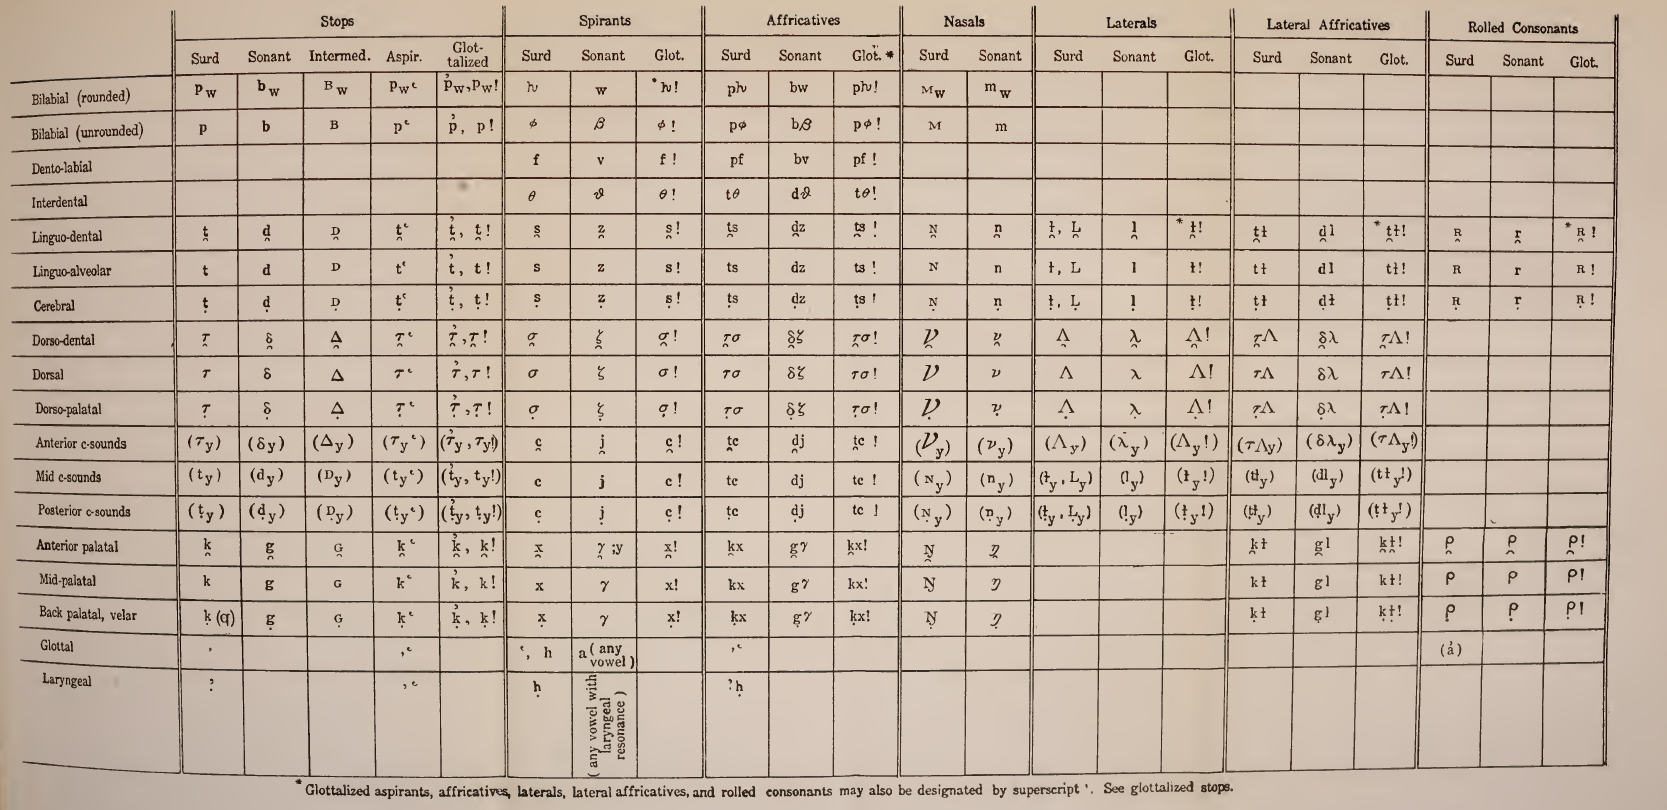
\includegraphics[width=1\linewidth]{jipa/images/americanistChart}
	\caption[Original chart of the Americanist Transcription System \parencite{boasPhoneticTranscriptionIndian1916}]{The original chart of the Americanist Transcription System \parencite[21--22]{boasPhoneticTranscriptionIndian1916} is not included in the original article. Rhotics are under the category ‘Rolled Consonants’. The small capitalized \textsc{d} is found among the ‘Stops’ category.}
	\label{fig:americanistchart}
\end{figure}


The ATS used the term ‘intermediate stop consonants’, that might be interpreted as taps, using the (small) capital grapheme D to represent them (the lower case d being reserved for the voiced apical stop).\footnote{A symbol for the flap ř exists as well. The tap and the flap were never intended to be contrasted by means of two symbols. While \textcite[88]{chomskyCurrentIssuesLinguistic1964} uses the symbol D for the tap (same as the symbol found in the original ATS but with a capital letter instead of a small capital), the flap ř might come from \textcite{smalleyManualArticulatoryPhonetics1963} who used it in opposition with the trill.}
Notably, the tap is considered as an allophone of plosives /t d/, and is not represented by an \textit{r}–based segment like in the Europeanist tradition. In the latter,  the symbol \textit{ɾ} is found to represent at the same time taps as allophones of rhotics and as allophones of plosives. In 1949, the Europeanist tradition, in its \textit{Principles of the International Phonetic Association being a description of the International Phonetic Alphabet and the manner of using it, illustrated by texts in 51 languages} \parencite{ipaPrinciplesInternationalPhonetic1949} notes for \textit{r}:

\begin{displayquote}
\textit{r}. Rolled \textit{r} as in Scottish English, Italian, Spanish, Russian. The letter is also used whenever possible to denote flapped \textit{r} (\textit{ɾ}), fricative \textit{r} (\textit{ɹ}) [sic], lingual fricationless continuant \textit{r} (\textit{ɹ}) , uvular rolled \textit{r} (\textit{ʀ}), uvular fricative \textit{r} (\textit{ʁ}) [sic] or the uvular frictionless continuant (\textit{ʁ}). \parencite[Section 26]{ipaPrinciplesInternationalPhonetic1949}
\end{displayquote}

There are also some clarification notes:

\begin{displayquote}
(d) The letter \textit{ʀ} may denote the fully rolled sound with two or more flaps of the uvula or the single–flap sound. In a language containing the two sounds as separate phonemes, the notation \textit{ʀʀ} is recommended for the fully rolled sound.

(e) The letter \textit{r} may, when convenient, replace \textit{ɹ}, \textit{ʀ} or \textit{ʁ} in the transcription of a language containing one of these three sounds but not a rolled lingual \textit{r}.

(f) The flapped sound \textit{ɾ} can generally be represented by \textit{r}. In a language such as Spanish, where a single flap and the fully rolled sound occur as separate phonemes, the notation \textit{rr} is recommended for the fully rolled sound. \parencite[Section 27]{ipaPrinciplesInternationalPhonetic1949}
\end{displayquote}

Thus, the symbol \textit{r} can be used to represent no less than 7 different phones with different manners and places of articulation (diacritics were not yet a norm at that time, so as to represent a  more open fricative or approximant, with the fricative \textit{ɹ} being next to \textit{θ} and \textit{ð}, and \textit{s} and \textit{z} in the 1949 table). The convention to duplicate the symbol does not seem clearly specified, but is left to the authors' interpretation. The use of a single symbol for these phones may be based on the idea that these sounds really belong to a single phonological class, called rhotics, which has been widely used in the literature \parencite{barryAnotherRtickle1997,scobbieVariable2006,magnusonStoryTwoVocal2007,chabotWhatWrongBeing2019} but without reaching a universal and consensual definition. While reflecting a certain theoretical stance, this ‘homonymy’ can lead to misunderstandings and to a potential bias favoring the interpretation of trill (or rolled) \textit{r} as the typical and most common phoneme represented by symbol \textit{r} despite a more nuanced situation.\\

The 1999 edition of the \textit{Handbook of the International Phonetic Association: A Guide to the Use of the International Phonetic Alphabet} \parencite{ipaHandbookInternationalPhonetic1999} says:

\begin{displayquote}
Trills are sounds like [r] is Spanish perro ‘dog’ in which the air is repeatedly interrupted by an articulator (in this case the tongue tip) vibrating in an airstream. A very short contact, similar in duration to one cycle of the vibration of a trill, is called a tap, such as the [ɾ] in Spanish pero ‘but’. \parencite[8]{ipaHandbookInternationalPhonetic1999}
\end{displayquote}
\begin{displayquote}
Note: most forms of English, French, German, Swedish do not have trills except in over–articulated speech, for instance when trying to be clear over a poor telephone line. \parencite[19]{ipaHandbookInternationalPhonetic1999}
\end{displayquote}
In this edition, there is no explicit guideline on using \textit{r} as a generic symbol to denote different phones, but there is no indication to avoid this practice, either.\\

In conclusion, the IPA mandates a generic use of the \textit{r} symbol that blurs what was actually analyzed: while it conveys the broad idea that this is a rhotic, it is left to the author(s) to somehow clarify the place(s) and manner(s) used. This imprecision, unfortunately, can be quite misleading for typological, comparative work, especially when large databases and quantitative methods are used (but even more focused, manual comparisons might be affected as well).

\subsection{‘Trills’ and ‘taps’}\label{subsec:trill_tap}

The phone alveolar trill is usually described in terms of articulation, acoustics and aerodynamics, and most of the authors refer to Spanish (or other Romance languages such as Catalan; Recasens \parencite*{recasensProductionCharacteristicsApicoalveolar1991}) for its characterization. In \textit{the Handbook of the International Phonetic Association} \parencite{ipaHandbookInternationalPhonetic1999}, the trill is described articulatorily, and the tap is described as similar to the trill but with one cycle only (using Spanish as reference) \parencite{ipaHandbookInternationalPhonetic1999}.\footnote{Please note that we do not make here a distinction between alveolar tap (‘a tap is a sound in which a brief contact between the articulators made by moving the active articulator directly towards the roof of the mouth’ \parencite[231]{ladefogedSoundsWorldLanguages1996}) and flap (‘a flap is a sound in which a brief contact between the articulators made by moving the active articulator tangentially to the site of the contact, so that it strikes the upper surface of the vocal tract in passing’ \parencite[231]{ladefogedSoundsWorldLanguages1996}), and we assume that both terms refer to the same sound. While this is clearly a simplification \parencite{derrickIndividualVariationEnglish2011}, it should not have any substantial consequences for our purposes here.}
One can wonder whether trills are produced in the same way across all languages that use them, and not just in those Romance examples. While not explicitly addressed, we may expect that [r] should refer to roughly the same speech sound in languages across the world.

On the phonemic level, it is cross–linguistically infrequent to find contrasts between two trills with different places of articulation \parencite{ladefogedLateralsTrills1977,maddiesonPatternsSounds1984}, but some languages, such as Russian \parencite{yanushevskayaRussian2015} and Toda \parencite{spajicTrillsToda1996}, are reported to contrast between an alveolar trill without secondary articulation and a palatalized alveolar trill. From an articulatory point of view, ‘trills can be produced with any of the three mobile articulators: the lips, the tongue, the uvula [...]’ \parencite[49]{ladefogedLateralsTrills1977}, but only the last two are usually considered to belong to the rhotic class, as \textit{r}–like segments, written with a <r> in the Latin–based alphabet. The lingual trill can be laminal or apical: for example, in the Illustrations of the IPA, laminal trills (also called fricative trills in Illustrations) can be found in Mbarrumbathama \parencite{verstraeteMbarrumbathamaLamalama2019} and in Czech \parencite{dankovicovaCzech1997, simackovaCzechSpokenBohemia2012}. Apical trills are found, for example, in Spanish, and are generally assumed to be the prototypical trills; they can be linguolabial, dental, alveolar or postalveolar, but linguists, in general, only consider the dental and the alveolar places \parencite{ladefogedLateralsTrills1977}. Solé’s studies \parencite*{solePhonologicalUniversalsTrilling1998,soleAerodynamicCharacteristicsTrills2002} of the aerodynamics of the trilling action made with the tip of the tongue in Spanish suggest that the initiation phase is critical:

\begin{displayquote}
The conditions for initiating lingual trilling involve (i) muscle contraction of the tongue to assume the position, shape and elasticity requirements and (ii) a sufficient pressure difference across the lingual constriction. Once trilling is initiated, tongue–tip vibration is maintained as a self–sustaining vibratory system. Articulatorily, trills exhibit more predorsum retraction than taps, thus leaving more room for the vertical movements of the tongue tip and blade, and more retracted alveolar closure. In addition, the tongue body is more highly constrained for the trill than for the tap and the former articulates less with neighboring vowels. \parencite[404]{solePhonologicalUniversalsTrilling1998}
\end{displayquote}

Two parts of the tongue are involved in the alveolar trill: the tip of the tongue, and the root of the tongue. Phonetic trills are produced with the tongue body more constrained and the predorsum more lowered than for taps \parencite{recasensStudyLightDAC1999}. The predorsum retraction leading to a pharyngeal constriction may be a characteristic of some rhotic segments including at least the trill \parencite{boyceAcquiringRhoticityLanguages2016} and could explain the late acquisition of trills observed crosslinguistically \parencite{mcleodChildrenConsonantAcquisition2018}.\\

Phonemic trills are no exceptions when it comes to allophony. Solé \parencite*[412]{solePhonologicalUniversalsTrilling1998} notes that in Spanish, taps, approximants and fricatives occur as allophones, and there is variation between dialects \parencite{pennyVariationChangeSpanish2000}. Variation in production is found in other well described languages. \textcite{rennickeVariationChangeRhotics2015} observes that in Brazilian Portuguese (which contrasts two rhotics), the rhotic allophonic family can be very large, as judged from productions ([r r̥ ɾ ɾ̥ ɾ̞ ɾ̞̥ ɹ j ɻ w ə ɚʰ ɹʰ jʰ ɻʰ ʀ ʁ χ ɦ h]); based on the Figure 8.1, p.239). \textcite{sebregtsSociophoneticsPhonologyDutch2014} for Dutch reports twenty possible variants and highlights the fact that taps that are highly frequent are not ‘failed trills or even successful trills with a single contact’ but intended as such. He favors the hypothesis that taps might historically originate from trills without excluding the possibility of a ‘reverse directionality’ \parencite[179]{sebregtsSociophoneticsPhonologyDutch2014}. The articulatory reduction and the reinterpretation of the allophonic alveolar trill can result in the emergence of allophones; for example, the change of place of articulation from alveolar to uvular, or the emergence of fricatives as ‘“failing” trills’ \parencite[412--413]{solePhonologicalUniversalsTrilling1998}. The interactions and relationships between different variants of the same phoneme /r/ are also studied (for example, for Greek \parencite{baltazaniManyFaces2013}, for Dutch \parencite{sebregtsSociophoneticsPhonologyDutch2014}, or for South–Tyrol Italian \parencite{spreaficoSociophoneticsBozenModelling2016}) in an attempt to understand the linguistic and social factors that may play a role in the variation found on the surface, and the place of the trill [r] in this allophone network.\\

Some authors suggest that, from an acoustic point of view (which is, to state the obvious, not necessarily the same as an articulatory point of view), a trill is basically a sequence (or series) of taps and, conversely, that a tap is a trill with a single period \parencite{lindauStory1985,ladefogedSoundsWorldLanguages1996}. However, there does not seem to be a consensus on the number of periods that an allophonic trill should have, varying from 2–3 closures up to 6–8, and it may depend not only on the variety, but also on the context and the speaker \parencite{henriksenAcousticCharacterizationPhonemic2010}. Moreover, the aforementioned references suggest that in a linguistic system one can observe a coexistence of a single-closure allophonic trill with a genuine tap, leading to another source of confusion. The phonetic alphabet does not capture these fine differences in the number of closures in part because there are no conventions on how to represent them.\\

One can note several conditioning factors that affect the distribution of the allophones mentioned above. The most important are probably the phonetic/ phonological environment and the broader context (i.e. the discourse settings and the communicative intentions). The phonetic and phonological environment includes the position within the syllable and the word, with intervocalic and final position favoring taps, while word– and syllable–initial positions favoring trills; trills are also more frequent in stressed syllables \parencite{eadesGayo2006,iskarousInteractionContrastProsody2010,mooneyBearnaisGascon2014}. There is indeed an association between stress and the increase in subglottal pressure \parencite{liebermanIntonationPerceptionLanguage1966}, with a minimum difference of 2 to 3 cm H$_2$O for voiced trills across the glottis \parencite{soleAerodynamicCharacteristicsTrills2002}. The wider context most frequently refers to careful or emphatic speech, and to the use of citation forms, all favoring the production of trills \parencite{breenCentralArrernte2005,bakerDariAfghanPersian2016}. Inter–speaker variation in the production of allophonic trills and taps is also somehow overlooked despite being widely accepted: ‘[...] taps are not produced in the same way in different languages nor are they always produced in the same way by different speakers of the same language’ \parencite[161]{lindauStory1985}. This ambiguous recognition status is probably related to a lack of studies addressing this type of variation. When considering the phonemic trill, an additional (sociolinguistic) source of inter–speaker variation is that individuals that fail to master the trill in languages that normatively use it, are usually considered as having a speech disorder \parencite{romano2013preliminary}, and may undergo speech therapy. Such individuals may systematically use sounds that are similar to the target trill but might be easier to articulate (e.g., alveolar approximants), but these substitution patterns seem to differ across languages and speakers (e.g., the allophonic palatal approximant [j] studied in \textcite{alfwaressRelationshipVocalTract2015} for native Arabic speakers).

\subsection{The cross–linguistic occurrence of ‘trills’}

Due to multiple reasons, which we detail below, we concur with Lindau’s \parencite*{lindauStory1985} assessment that:

\begin{displayquote}
An actual trill realization of an /r/ is not as common as might be expected from descriptions of languages, where an /r/ is often labeled as a ‘trill’. Even in languages where a possible realization is a trill, not all the speakers use a trill, and the speakers that do, have a tap and approximant allophones as well as the trill. \parencite[161]{lindauStory1985}
\end{displayquote}

In fact, the orthography used by the IPA – based on the Latin alphabet extended with additional symbols – probably had a huge impact: some symbols from the extended set might appear ‘stranger’ than others, encouraging the preponderant use of the ‘basic’ Latin IPA characters. It seems that some authors may have a preference towards the use of the symbol \textit{r} even if the actual sound is realized with one closure only, while others use the same symbol to report all ‘\textit{r}–like’ sounds (\textit{r} in some cases referring to speech sounds made at the uvular place of articulation). The historical development of the IPA itself may have contributed to this situation, as there was no symbol for the tap before 1908, with \textit{ɹ} being used for the ‘untrilled lingual \textit{r}’ (the alveolar approximant). Even after its proposal in 1908, the symbol \textit{ɾ} had to wait until 1928 before appearing in Le Maître Phonétique in the IPA chart included in reprinted Daniel Jones' article \textit{Das System der Association Phonétique Internationale (Weltlautschriftverein)} \parencite*{jonesSystemAssociationPhonetique1928}.\\

\begin{figure}
	\centering
	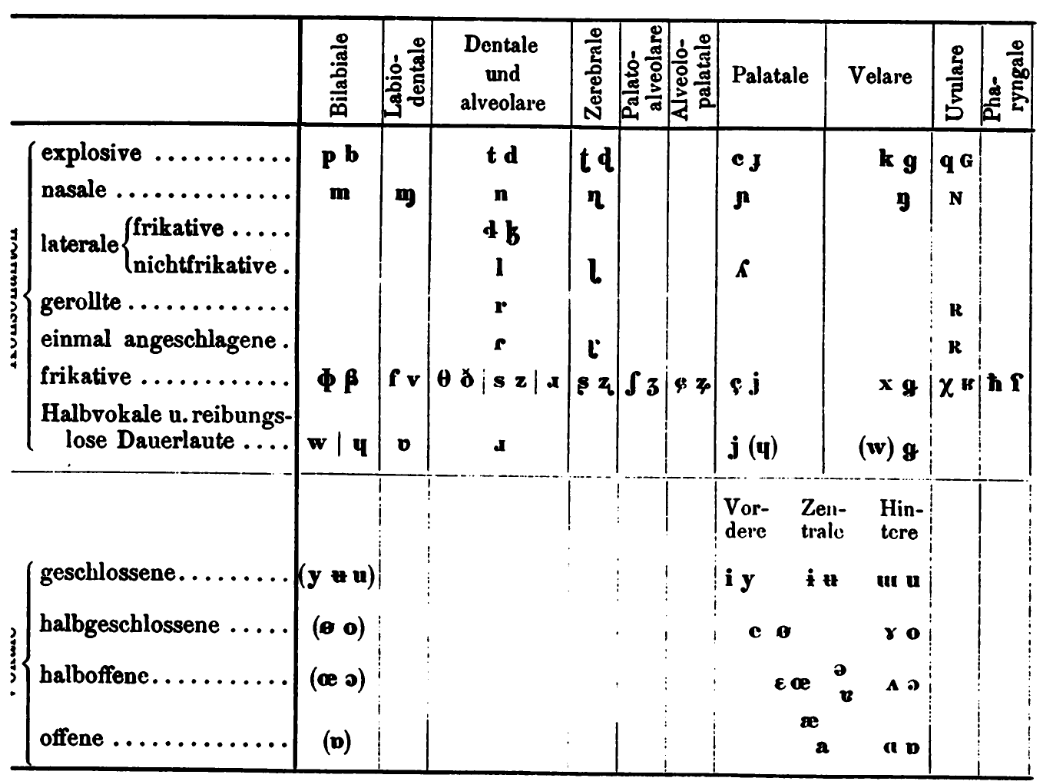
\includegraphics[width=1\linewidth]{jipa/images/jones_table}
	\caption[Chart of consonants in German of the International Phonetic Association by \parencite{jonesSystemAssociationPhonetique1928}]{The chart of consonants in German of the International Phonetic Association by \parencite[23]{jonesSystemAssociationPhonetique1928}. It is not included in the original article. ‘gerollte’ can be translated by ‘rolled’ and ‘einmal angeschlagene’ by ‘once struck’.}
	\label{fig:jonestable}
\end{figure}

While in some languages, such as Spanish and Catalan, the presence of phonemic trills and taps has been intensely studied, for many others this is still not the case. This is further complicated by contextual, dialectal, sociolectal and idiolectal variation, as well as by language contact and ‘rarity’: for example, in Bearnais (Gascon), a standard French [ʁ] might be produced as an allophone of the apical rhotics /r/ and /ɾ/  \parencite{mooneyBearnaisGascon2014}; and in Isthmus (Juchitán) Zapotec, an alveolar trill is present in ‘less than a half dozen words’ \parencite[366]{pickettIsthmusJuchitanZapotec2010}. In some language varieties, an alveolar trill allophone of the phonemic rhotic may be stigmatized (as in, for example, Japanese \parencite{labrunePhonologyJapanese2012,ooigawaPerceptionItalianLiquids2015,vanceSoundsJapanese2008} and French  \parencite{prematRouleFrancaisDans2018}. The allophonic tap can also be a source of stigmatization as in Cagliari Sardinian where it is an ‘stigmatized’ allophone of the alveolar plosives but not for the intervocalic /r/ \parencite{mereuCagliariSardinian2019}. Scottish English is a good illustration of the discrepancy between reality and a metalinguistic representation biased in favor of trills: it turns out that trills are not common in Scottish English. \textcite[57]{lawsonSocioArticulatoryStudyScottish2014} report that ‘many speakers, when questioned, will say that a typical Scottish /r/ is a trilled /r/, even though this is rarely the case nowadays’, and many recent studies systematically show the rarity of trilling in Scottish English \parencite{pukliInvestigationSociophonetiqueAnglais2006,stuart-smithDerhoticisationScottishEnglish2014,jauriberryRhotiquesRhoticiteEcosse2016}. The large variation observed in the phonemic trill may be in part explained by the fact that allophonic trills are articulatorily more complex than allophonic taps (the latter being acquired earlier than the former, \parencite{mcleodChildrenConsonantAcquisition2018}), require more energy and a precise control of the parameters involved in its aerodynamics, which can lead to trilling failure.\\

Therefore, it seems that more than a century after the publications of the first international guidelines on phonetic transcription, the way the symbol \textit{r} is used throughout the linguistic community is still not consistent and universally shared. We argue here that this situation is highly detrimental and significantly hinders the capacity to develop a typology of the [r] sound and of the rhotics from a phonetic perspective. Answering questions such as whether or not [r] is rare becomes unnecessarily complicated, and querying databases needs extra care to identify and control for the noise induced by the (sometimes implicit) use of different guidelines and expectations concerning the way sounds should be represented.

\section{Data and methods}

To address the problem with the generic use of \textit{r}, we conducted a full analysis of all the articles published in the peer–reviewed \textit{Journal of the International Phonetic Association} in the collection \textit{Illustrations of the IPA}.\footnote{ISSN: 0025–1003 for the printed, and 1475–3502 for the \href{https://www.cambridge.org/core/journals/journal-of-the-international-phonetic-association}{online editions}}
The journal began at the end of the 19th century, initially titled \textit{Le Maître Phonétique} and fully written in the \textit{Alphabet Phonétique International} (API), or \textit{International Phonetic Alphabet} (IPA) in English, changing its name to JIPA only in 1971, and moving away from articles written in IPA (in different languages) and towards standard orthographies. The \textit{Illustrations of the IPA} section first appeared in \textit{JIPA}'s 20th volume in 1990, following a decision of the 1989 Kiel Convention \parencites[77--80]{ipaIllustrationsIPA1990,roachReport1989Kiel1989}. Since then, \textit{Illustrations} has been compiled in two volumes, in 1995 and 1999. Prior to the creation of the \textit{Illustrations} section, transcriptions of ‘The North Wind and the Sun’, dating back to the earliest days of \textit{Le Maître Phonétique}, were published variously in \textit{The Principles of the International Phonetic} Association \parencite{ipaPrinciplesInternationalPhonetic1949} and particular volumes under various sections, such as \textit{spesimɛn} (Specimen).\\

\begin{figure}
	\centering
	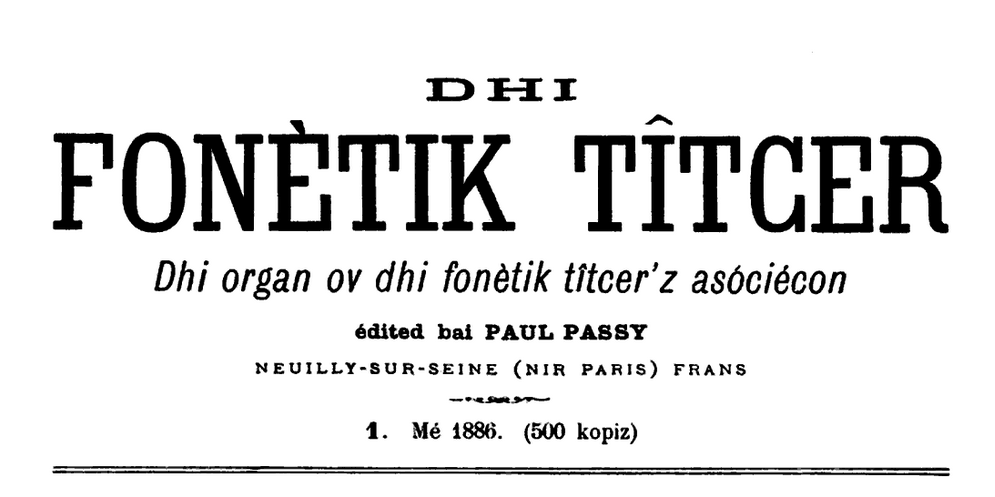
\includegraphics[width=1\linewidth]{jipa/images/phonetic_teacher}
	\caption[Illustration of the title of first issue of the journal of the association ‘lə mɛ${:}$trɘ fɔnetik’]{As the International Phonetic Association evolved \parencite{esling40thAnniversaryJIPA2010}, so did its transcription system and its journal. This title of first issue of the journal of the association ‘lə mɛ${:}$trɘ fɔnetik’ / ‘dhi fonètik tîtcer’ is not included in the original article.}
	\label{fig:phoneticteacher}
\end{figure}

The original aim of \textit{Illustrations} was to offer a linguistic foundation to the written symbols, or graphemes, chosen to represent the sounds of spoken languages, with each illustration focusing on a single variety (‘language’, dialect or sociolect). The idea was and still is that each such contribution should define the phonemic inventory (or, if not possible, at least to sketch a first version) using the IPA symbols. Some illustrations also contain a summary of the studies on the variety, and a brief sociolinguistic sketch (including speaker population size, socioeconomic status of the informants, bi–/multilingualism, and relationships to an official variety). Over the years, \textit{Illustrations} has provided invaluable insights into the sound systems of a large number of languages and varieties. \\

Each illustration provides a narrative which is, in general, based on a single speaker who pronounces the poem ‘The North Wind and the Sun’ in their own variety, but some authors chose to include a different story. This narrative is recorded and then transcribed. The most recent instructions for contributors \parencite{ipaInstructionsContributors2021} indicate that the transcription must be ‘phonemic’ (highlighting the contrasts in the language) but that a ‘narrow’ transcription can also be added (highlighting the phonetic specificities of the variety and/or of the speaker(s)’s idiolect(s)).

\subsection{Data collection}\label{subsec:data_coll}

The primary data consists of all the relevant information extracted from illustrations available on the \textit{JIPA} website. Due to a change of style after 2000, when Cambridge University took over the production of JIPA \parencite{ipaPublicationJournalInternational2000}, we split them into those published before 2000 (42 illustrations), and those published between 2000 and 2020 (168 illustrations). We checked the consistency of the pre–2000 illustrations with their re–edited version in the \textit{Handbook of the International Phonetic Alphabet: A guide to the use of the International Phonetic Alphabet} in 1999 (IPA, 1999), and we included two additional illustrations present only in this source but absent from the \textit{JIPA} website (American English by Ladefoged \parencite*[41--44]{ipaHandbookInternationalPhonetic1999} and Portuguese (European) by Cruz \parencite*[126--130]{ipaHandbookInternationalPhonetic1999}), resulting in a total of 213 illustrations, including 46 published before 2000.\\

We compiled the extracted information in a table (in CSV format, available in the Supplementary Materials accompanying the original article), with the following information:

\begin{itemize}
	\item[–] the title of the illustration (which corresponds to the name of the lect/variety),
	\item[–] the year of publication of the illustration (for those recent illustrations included in the First view section of the JIPA website \parencite[472]{arvanitiEditorialReportJIPA2019}, we used the year the illustration appeared online which does not necessarily coincide with the year of publication),
	\item[–] the author’s/authors’ name(s), affiliation(s), e–mail address(es),
	\item[–] the geographical area, the country/countries, and the specific region(s) in which the variety is spoken,
	\item[–] the size of the speaker population, if available,
	\item[–] if available, information concerning the informant(s), such as the sex, age and
	socio–economic status,
	\item[–] the section(s) of the narrative transcription which allowed us to infer if the transcription is ‘phonemic’ (i.e., using a phoneme representation, usually known as a ‘broad transcription’) or rather ‘phonetic’ (i.e., using phonetic representation, usually known as a ‘narrow transcription’) \parencite[Section 5]{ipaHandbookInternationalPhonetic1999}. While some illustrations have one transcription only, a few of them include both phonemic and phonetic transcriptions (for more details, see the \autoref{subsec:pht_phm}).
\end{itemize} 

We manually added the location where the variety is spoken, and, when there was no indication of the actual geographical coordinates, we used Google maps and Open Street maps to estimate the latitude and longitude, starting from the reported name of the place. We used a broad classification of macroareas based on that proposed by Glottolog \parencite{glottolog}.

\subsection{Defining and coding ‘\textit{r}–like’ sounds}

We decided to focus on two characters \textit{r} and \textit{ɾ} (respectively lower–case R and fish–hook R [\cite{pullum1996phonetic}]) and the characters derived from these through the addition of diacritic(s). In our analysis we refer to the lower–case R as the \textsc{trill}, and to the fish–hook R as the \textsc{tap}.\\

We looked for their presence in the consonant chart, and the transcription(s) of a narrative given at the end of the illustrations. We then considered the ‘descriptive labels’, the way authors refer to symbols, following, in most cases, the phonetic categories given to the symbols in the consonant chart found at the beginning of each illustration (place of articulation, manner of articulation and voicing). For some older illustrations no such chart is given, leading us to retrieve the labels from the indications present in the text. Our analysis is focused on the alveolar trill and the alveolar tap, leaving the other rhotics for  future studies, but we nevertheless listed the other segments mentioned in the illustrations when they can potentially be considered as ‘rhotics’ based on \textcite{magnusonStoryTwoVocal2007}‘s classification (for example \textit{ɹ}, \textit{ɻ~~}, \textit{ɽ}, \textit{ʀ}, \textit{ʁ}), to provide an overview of the rhotics and ‘\textit{r}–like’ sounds present in the illustrations and to facilitate future work. 

\subsection{Counting ‘\textit{r}–like’ sounds}

As we are mostly interested in the use of trill and tap in the transcribed narrations of Illustrations here, we  manually counted them specifically focusing on:

\begin{itemize}
	\item[–] the number n$_\textrm{[r]}$ of tokens of r in the phonetic transcription
	\item[–] the number n$_\textrm{/r/}$ of tokens of r in the phonemic transcription
	\item[–] the number n$_\textrm{[ɾ]}$ of tokens of ɾ in the phonetic transcription
	\item[–] the number n$_\textrm{/ɾ/}$ of tokens of ɾ in the phonemic transcription
	\item[–] the  number n$_\textrm{ʀ}$ of rhotic tokens: this is based on the segments we considered as rhotics in the transcriptions given by the authors. We looked for the different symbols that were used for the trill, tap, and other \textit{r}–based segments, checking what the authors wrote about whether we should consider them as rhotics or not (for example, we excluded from this count the \textit{ɾ} in phonetic transcriptions when they were an allophone of a plosive). In some cases, we looked at the orthographic transcription that was provided by the authors to give us clues about <r> segments that could be omitted or realized differently from what was expected. When several transcriptions are provided, we have used the highest number n$_\textrm{ʀ}$ across the different transcriptions.
\end{itemize} 

An additional logical variable denoting the presence or absence of <r> in the orthographic system of the language or in the transliteration was added if available. For example, in some illustrations where the language described uses a Cyrillic alphabet, we find in the transliterations <r> standing for <p>, in which case we consider that the language does contain <r> in its orthography. \\

Although this data was collected by a single coder (RA), this was done in several separate ‘rounds’, which enabled quality checking and, if necessary, correction of earlier rounds in subsequent later rounds. The first round involved the collection of metadata for the illustrations and segments of interest; the second involved the manual addition of geographic locations. The collection of quantitative data was done over two rounds, which consisted of counting \textit{r} tokens in the transcriptions, followed by counting \textit{ɾ} tokens.

\subsection{Counting all segments n$_\textrm{Seg}$}

Finally, in order to normalize the number of occurrences of rhotics across the illustrations, we also counted the total number of segments in each transcription. Although all the transcriptions come from \textit{Illustrations}, there were inconsistencies in the format in which we recovered them:

\begin{itemize}
	\item[–] some transcriptions are available in text format (.txt) from \citeauthor{bairdBlowingWindUsing2021} (in press) (available on: \href{https://github.com/SimonGreenhill/jipa}{\texttt{https://github.com/} \texttt{SimonGreenhill/jipa}})
	\item[–] when possible, transcriptions were copy–pasted from the PDF of the illustrations or from the \textit{Illustrations} web page hosted by the \textit{Journal of the IPA}
	\item[–] some transcriptions from which copy–pasting was not possible were submitted to Optical character recognition (OCR) using the R package \texttt{tesser}-\texttt{act} \parencite{ooms2019tesseract} and corrected for potential errors or were manually typed.
\end{itemize}

If there was more than one transcription in an illustration (for example, one phonemic and one phonetic transcription, or for different varieties), we counted  the number of segments in the broadest transcription available, or by averaging the counts found in the transcriptions when they had the same level of phonetic precision. We wrote an R script to automatically count the alphabetical segments, using regular expressions excluding numbers, diacritics, second manners of articulation, suprasegmental symbols and punctuation.

\subsection{Phonetic and phonemic transcriptions}\label{subsec:pht_phm}

One of the most important and tedious steps was to classify the transcriptions according to their degree of detail. For this, we decided to look specifically at the information provided by the authors, mostly in the section headers, without any interpretations or inferences of our own. Because of the great variability in the naming of the section headers, it was nevertheless necessary to harmonize them. Therefore, we defined a binary distinction between ‘phonemic’ and ‘phonetic’ transcriptions, as follows. A phonetic transcription is inferred for section headers containing the terms ‘phonetic’, ‘narrow’, ‘allophonic’, ‘semi–narrow’, and/or ‘detailed’, while a phonemic transcription corresponds to the sections containing the following terms ‘phonemic’ and/or ‘broad’. In some cases, the authors specify that their transcription was either ‘broad phonetic’ or ‘narrow phonemic’ [sic]; here, we only kept the terms ‘phonetic’ and ‘phonemic’ to characterize these transcriptions.\\

73 transcriptions were still difficult to classify due to a lack of information, in which case, by default, we made the choice to systematically consider the transcriptions phonetic. This stems from the assumption that the purpose of Illustrations is to convey the phonetic realization of the language, as it is explicitly mentioned in the report on the 1989 Kiel Convention that the transcription should represent ‘what is actually recorded on the tape rather than an idealization of what might have been uttered’ \parencite[77]{roachReport1989Kiel1989}, even if this representation may be rather broad.\footnote{We have performed another analysis on the recommendation of the associate editor (available in the Supplementary Materials of the original article). The coding aimed at comparing the symbols present in the consonant chart and those present in the narrative transcription. If some segments were present in the narrative but not in the consonant chart, then the transcription could be considered phonetic. Of the 73 transcriptions, 31 were reinterpreted as phonemic (and 42 as phonetic. Working on a case by case basis poses the problem of adding a new bias in defining what is a phonetic and phonemic transcription when in most cases it is a mixture of both with some phonological classes being more detailed than others. When focusing on illustrations that have an \textit{r} somewhere in the transcription (or in the consonant chart), we find that 46 illustrations do not specify if the transcription is phonemic or phonetic. Of these 46 illustrations, 14 transcriptions were considered phonemic and 32 were considered phonetic.} This methodological choice is furthermore coherent with an approach in which the burden of the proof is ours: apparent trills are considered as trills as long as we cannot provide any strong arguments in favor of a non–trilled interpretation. 

\section{Results}

\subsection{General results}

\subsubsection{Year of publication}

It can be seen in \autoref{fig:graphyearjipa} that the Illustrations section started to be systematically published each year in 1990, with rather sporadic occurrences before this date. In total, we collected 213 illustrations covering 51 years (from 1971 to 2021), ranging between 1 and 22 per year with an average of 5.3. There is a difference between the date of publication on the Cambridge website and the date of publication in a \textit{JIPA} issue, usually about once year (see \autoref{subsec:data_coll} for details concerning the date of appearance in FirstView vs the publication date).

\begin{figure}
	\centering
	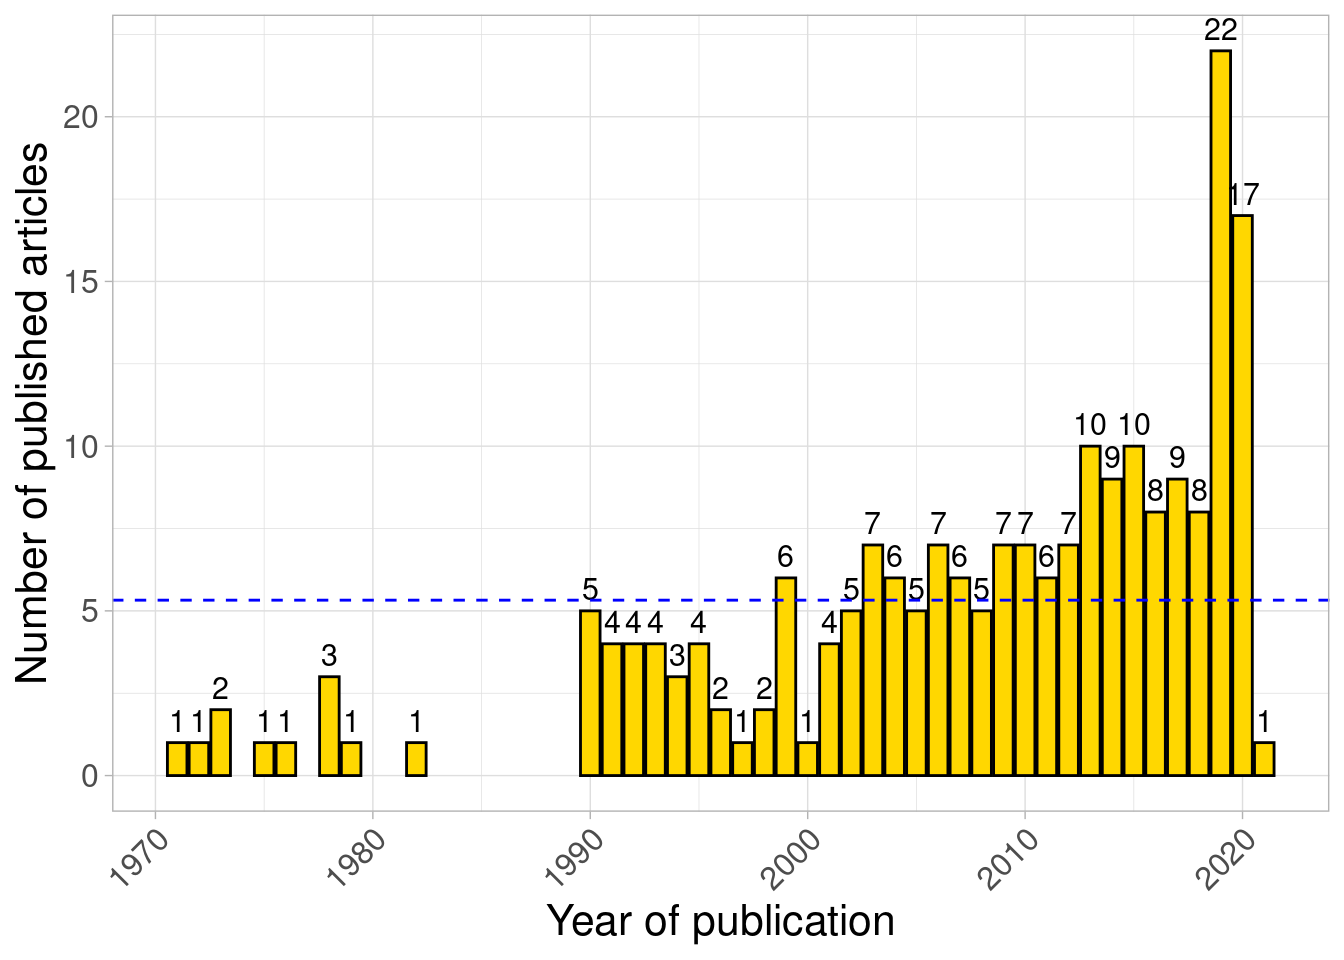
\includegraphics[width=1\linewidth]{jipa/images/graph_year_JIPA}
	\caption[Numbers of \textit{Illustrations of the IPA} publications per year]{Numbers of publications per year (yellow bars) with their average across all years (blue dashed line). Please note that some very recent illustrations might not yet be included in an official issue but only available on the journal’s website as FirstView. The figure does include First View articles with their online publication year.}
	\label{fig:graphyearjipa}
\end{figure}

\subsubsection{Informant characteristics}

For our purposes here, there might be speaker–related differences that are relevant, such as in age and gender (\autoref{fig:graphagejipa}). It is not clear if many authors are aware of any idiosyncrasies their informant(s) may have: this can be so because this is not the purpose of their illustration, or because they do not consider this as an important aspect when capturing the overall phonology/phonetics of the variety. In some cases, the authors explicitly state that they want speakers as ‘representative of the variety’ as possible \parencite[109]{namboodiripadMalayalamNamboodiriDialect2017a}.\\

Finally, since the authors are themselves academics, they tend to select speakers that are familiar with this environment, so most informants are considered as (well) educated and with a ‘correct’ pronunciation (according to the authors). Because the accessibility of the informants is an important factor, it is not uncommon for them to be students, researchers (some being the authors themselves) or teachers.

\begin{figure}
	\centering
	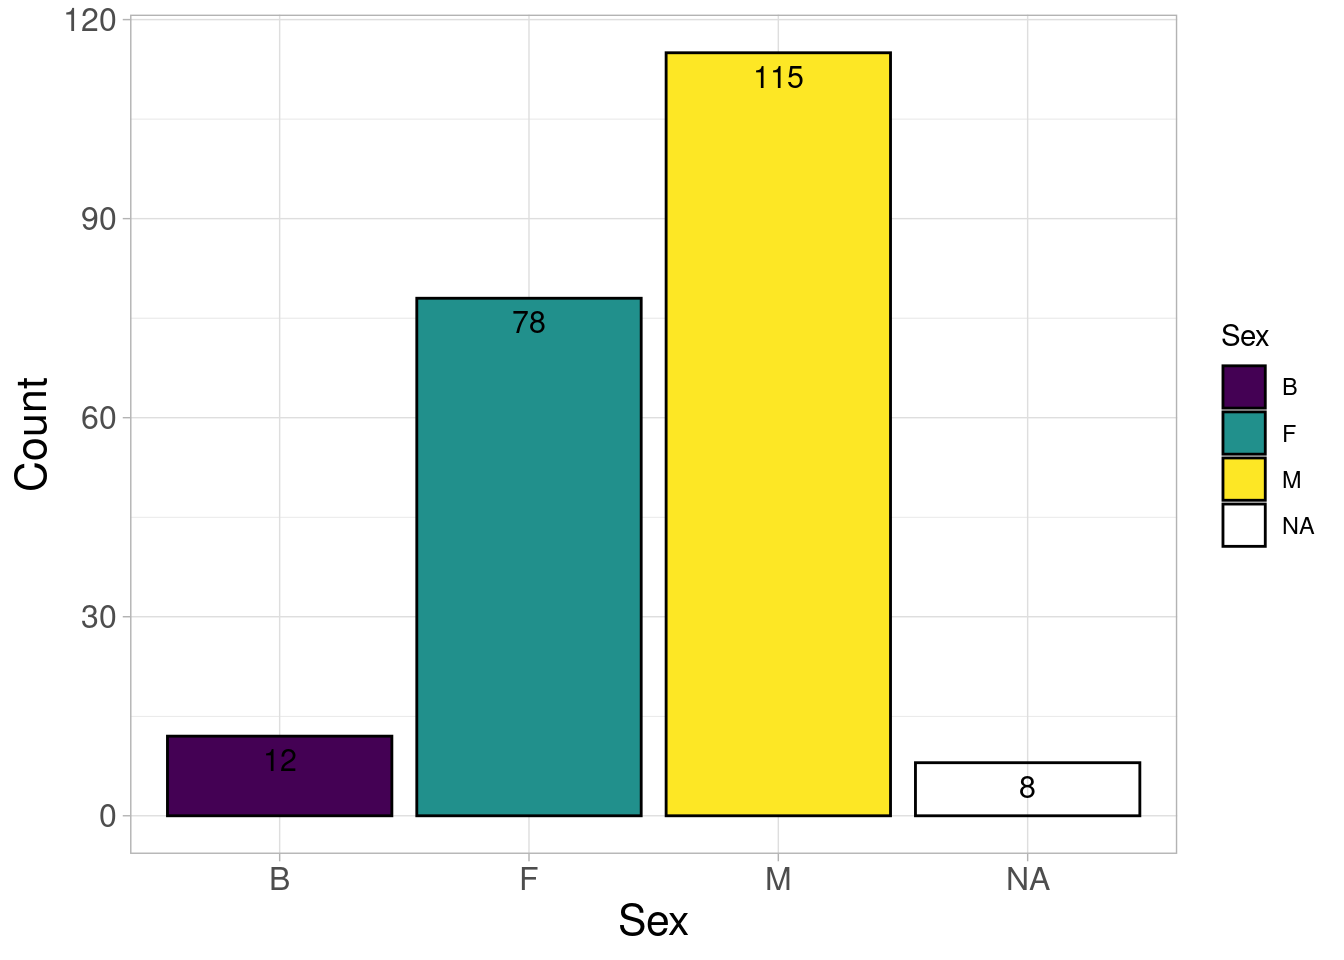
\includegraphics[width=0.475\linewidth]{jipa/images/graph_informant_JIPA}
	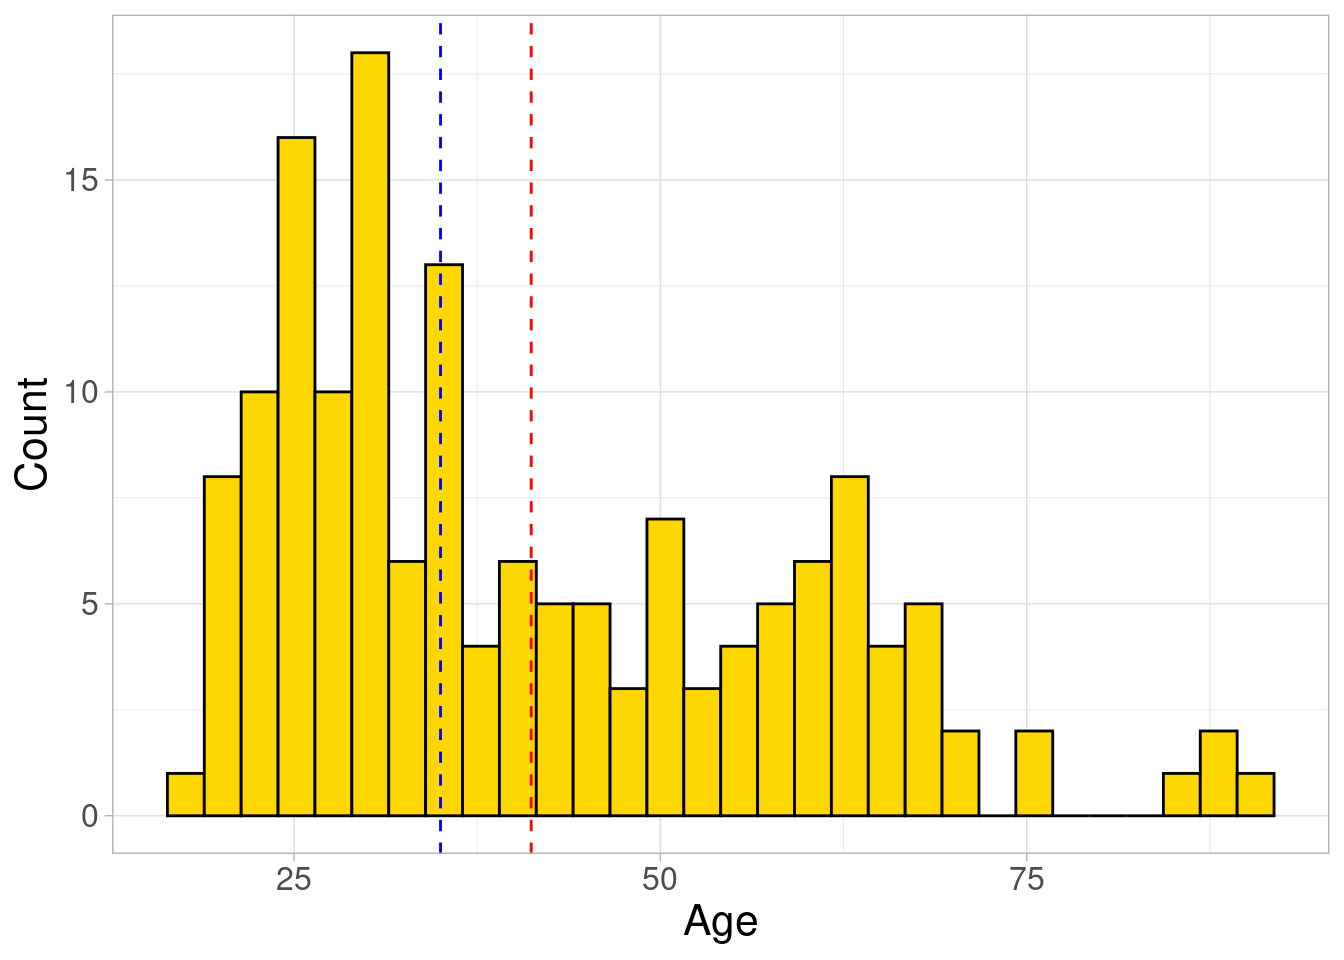
\includegraphics[width=0.475\linewidth]{jipa/images/graph_age_JIPA}
	\caption[Informant characteristics of the \textit{Illustrations of the IPA}]{Informant characteristics. Left: the distribution of informants' sex (F = female, M = male, B = both, i.e. the recording of at least 1M \& 1F used for the transcription, NA = data not communicated). Right: the distribution of the age of the informants, with mean 41 (red dashed line) and median 35 (blue dashed line).}
	\label{fig:graphagejipa}
\end{figure}


\subsubsection{Geographic distribution, families and population size}

There is an over–representation of Eurasian languages, in particular Indo–European languages, and just a few Australian languages (see Figures \ref{fig:graphfamiliesjipa} and \ref{fig:graphmacroareajipa}). Among the illustrations reviewed, a few languages are spoken by large populations and a few have very small speaker populations: the population of a variety covered by Illustrations is about 12,000,000 speakers on average, with a median of 175,000 (\autoref{fig:graphpopulationjipa}).

\begin{figure}
	\centering
	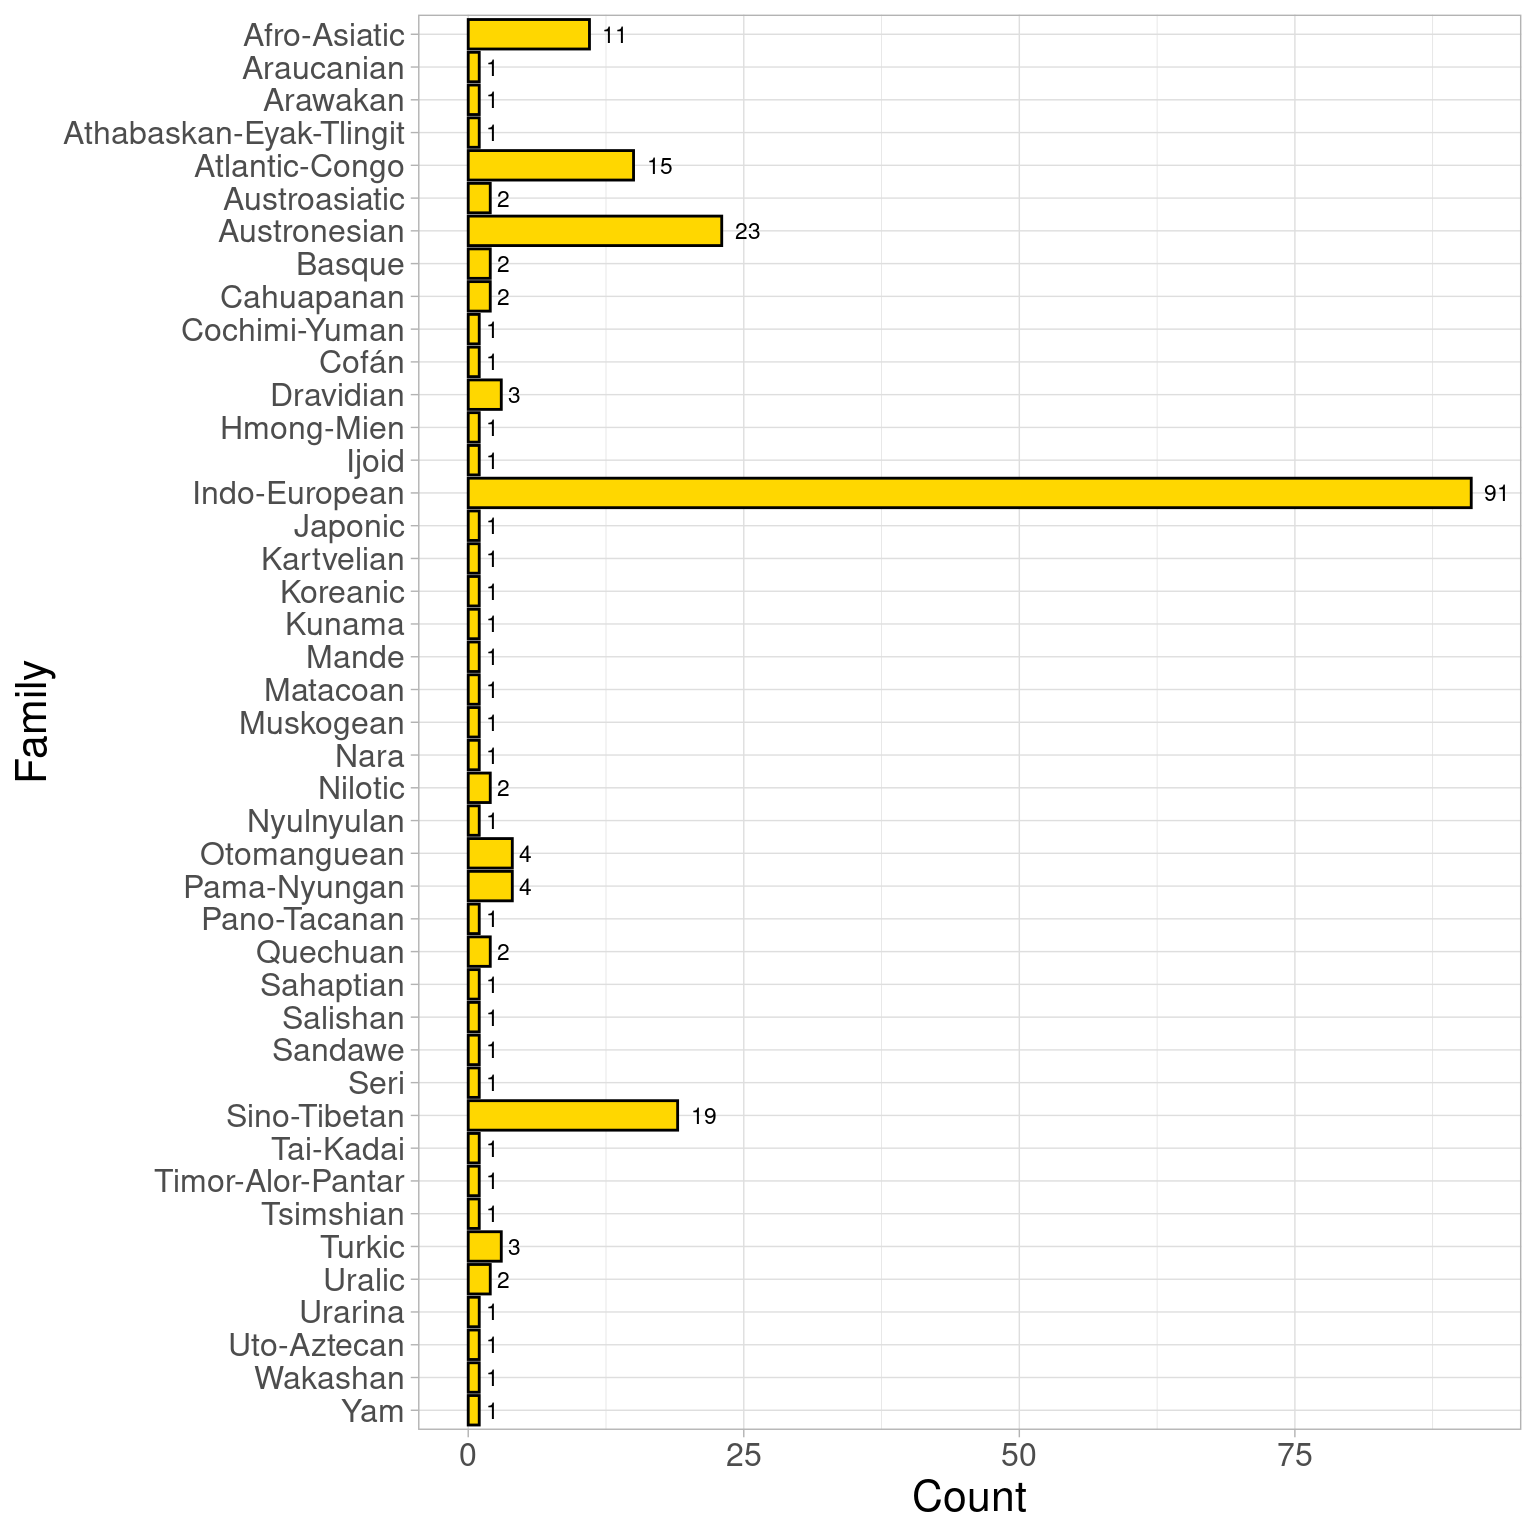
\includegraphics[width=1\linewidth]{jipa/images/graph_families_JIPA}
	\caption[Distribution of languages by family]{Distribution of languages by family based on family classifications in Glottolog \parencite{glottolog}}
	\label{fig:graphfamiliesjipa}
\end{figure}

\begin{figure}
	\centering
	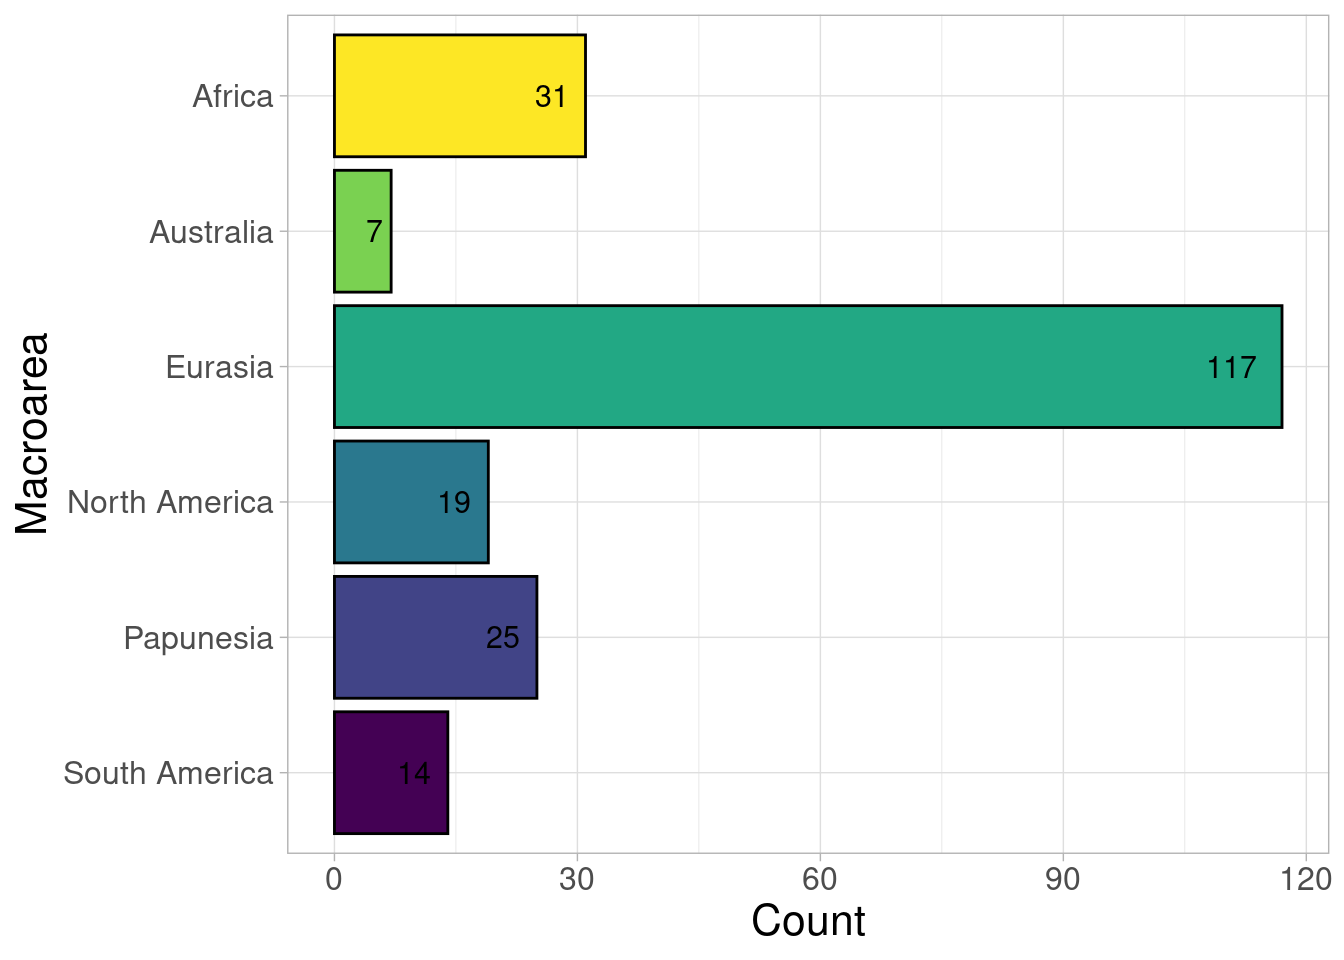
\includegraphics[width=1\linewidth]{jipa/images/graph_macroarea_JIPA}
	\caption[Distribution of languages by macroarea]{Distribution of languages by macroarea.}
	\label{fig:graphmacroareajipa}
\end{figure}

\begin{figure}
	\centering
	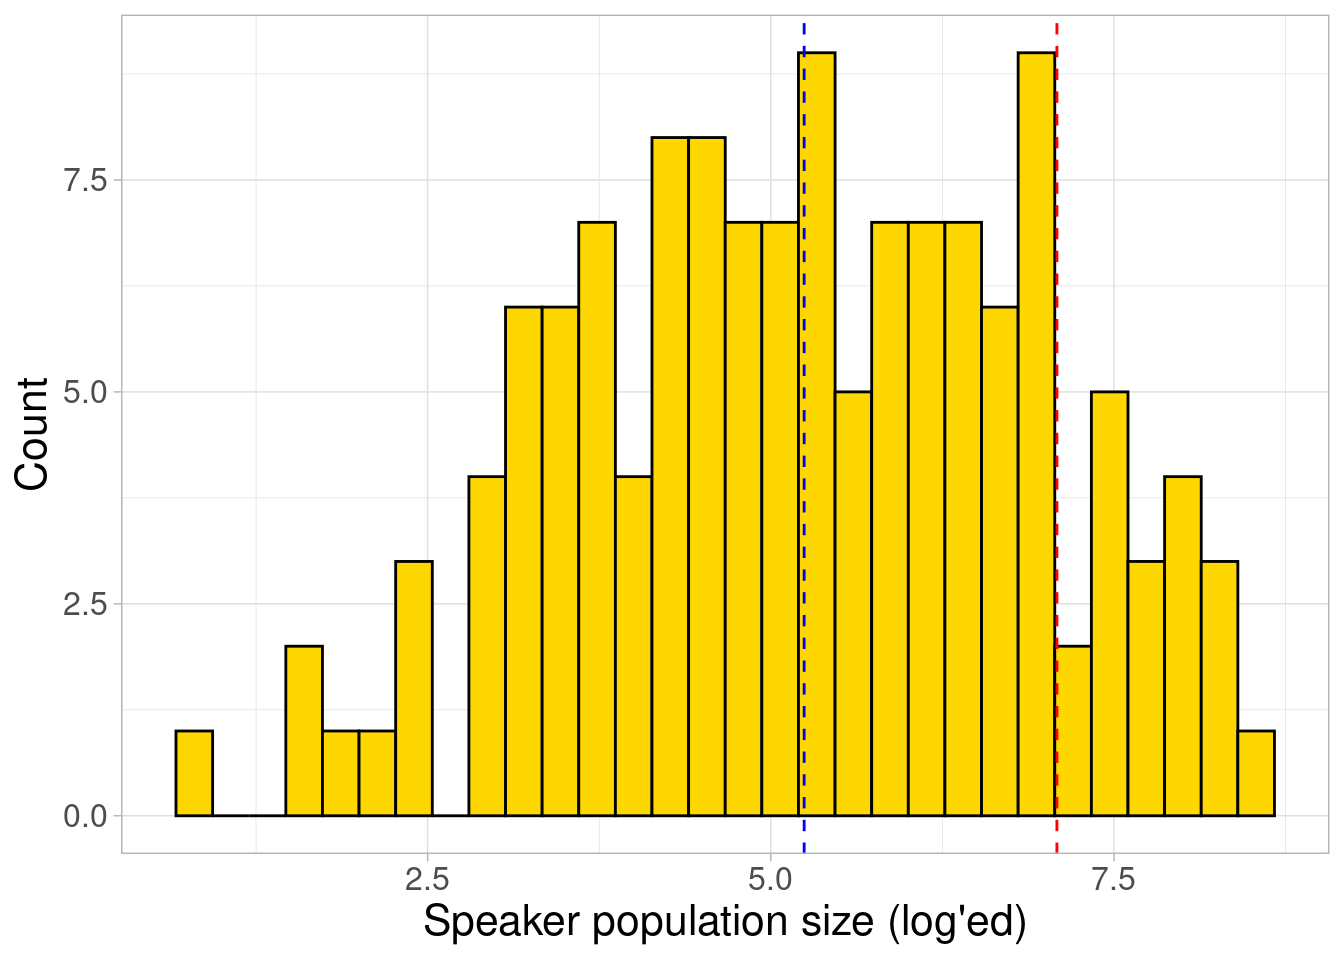
\includegraphics[width=0.7\linewidth]{jipa/images/graph_population_JIPA}
	\caption[Distribution of the log speaker population size]{The distribution of the log speaker population size, showing the mean (12,000,000 or 7.08 on the log scale; red dashed line) and the median (175,000 or 5.24 on log scale blue dashed line).}
	\label{fig:graphpopulationjipa}
\end{figure}

\subsection{Transcriptions}

\subsubsection{Phonetic and phonemic transcriptions}

Of the 213 illustrations, most had only one type of transcription (120 only had a phonetic transcription and 38 only a phonemic one) while 54 had both (phonetic and phonemic). The latter are the most informative for comparing the choice of the phonemes with their actual phonetic realizations. Finally, one single illustration did not have any transcribed narrative, this illustration corresponding to ‘Notes of a Westmeath dialect’ published in 1971 in the first volume of the \textit{Journal of the International Phonetic Alphabet}. 

\subsubsection{Orthographic transcription and transliteration}

Among the illustrations, there are several orthographic systems besides the Latin alphabet, and some of the studied languages of oral tradition do not have any orthographic system. Of the 213 illustrations, there are 134 (63\%) where we found an <r> in the orthography or in the transliteration. Among these, there are 47 (35\%) languages where a double <rr> was used (we do not exclude the possibility that other languages could also use <rr> in general, but the short length of the narrative does not allow us to provide a definite answer). There are 13 (6\%) illustrations where the language does not have an <r> in the orthography, and 66 (31\%) where either the language has no written tradition, or does not use the Latin alphabet and does not provide any transliteration in the Latin alphabet.

\subsection{‘\textit{r}–like’ sounds}

\subsubsection{\textit{r} in transcriptions}

We focus on the illustrations where the symbol \textit{r} is present: there are 136 illustrations (64\%) where \textit{r} is present in the consonant chart (105 illustrations) or there is at least an [r] or an /r/ in one of the narrative transcriptions (31 illustrations). The analyses presented in the rest of the article are based on this corpus. Among the 105 illustrations of the first type, 84 associated \textit{r} with the ‘trill’ or ‘rolled’ manner of articulation, based on the descriptive label derived from the consonant chart. In 16 cases, the usage of \textit{r} does not match with an actual trill description. An overview of the consonant charts leads us to consider that the \textit{r} is used for several manners of articulation (as an ‘approximant’, ‘tap or flap’, ‘plain tap’, ‘flap’, ‘fricative or approximant’), different places of articulation (ranging from ‘dental’ to ‘velar’), or sometimes is only just (under)specified as a ‘rhotic’. As an example, in the Shipibo illustration \parencite[282]{valenzuelaShipibo2001} it is stated that ‘[t]he symbol /r/, chosen for its simplicity, also represents a highly variable segment’. There are also 5 cases where there is no descriptive label that can be derived from the consonant chart or the illustration, preventing us from inferring what r stands for. We did not change the symbols when the \textit{r} did not match with an actual trill description.

We therefore divide the illustrations in three categories according to the type of transcription they include, and we present below the results per category, starting with the more informative with regard to phonetic substance.

\paragraph{Illustrations with both phonemic and phonetic transcriptions}

The first category includes 37 illustrations where the authors provide both phonemic and phonetic transcriptions, and which include at least one occurrence of an \textit{r} either in one of the transcriptions or in the consonant chart. Having both these transcriptions allows us to compare the phonemic transcription (which is the result of the linguistic analysis of which contrasts are important in the language) and the phonetic transcription (which arguably should be closer to the phonetic reality of what the speakers actually produced).

\begin{figure}
	\centering
	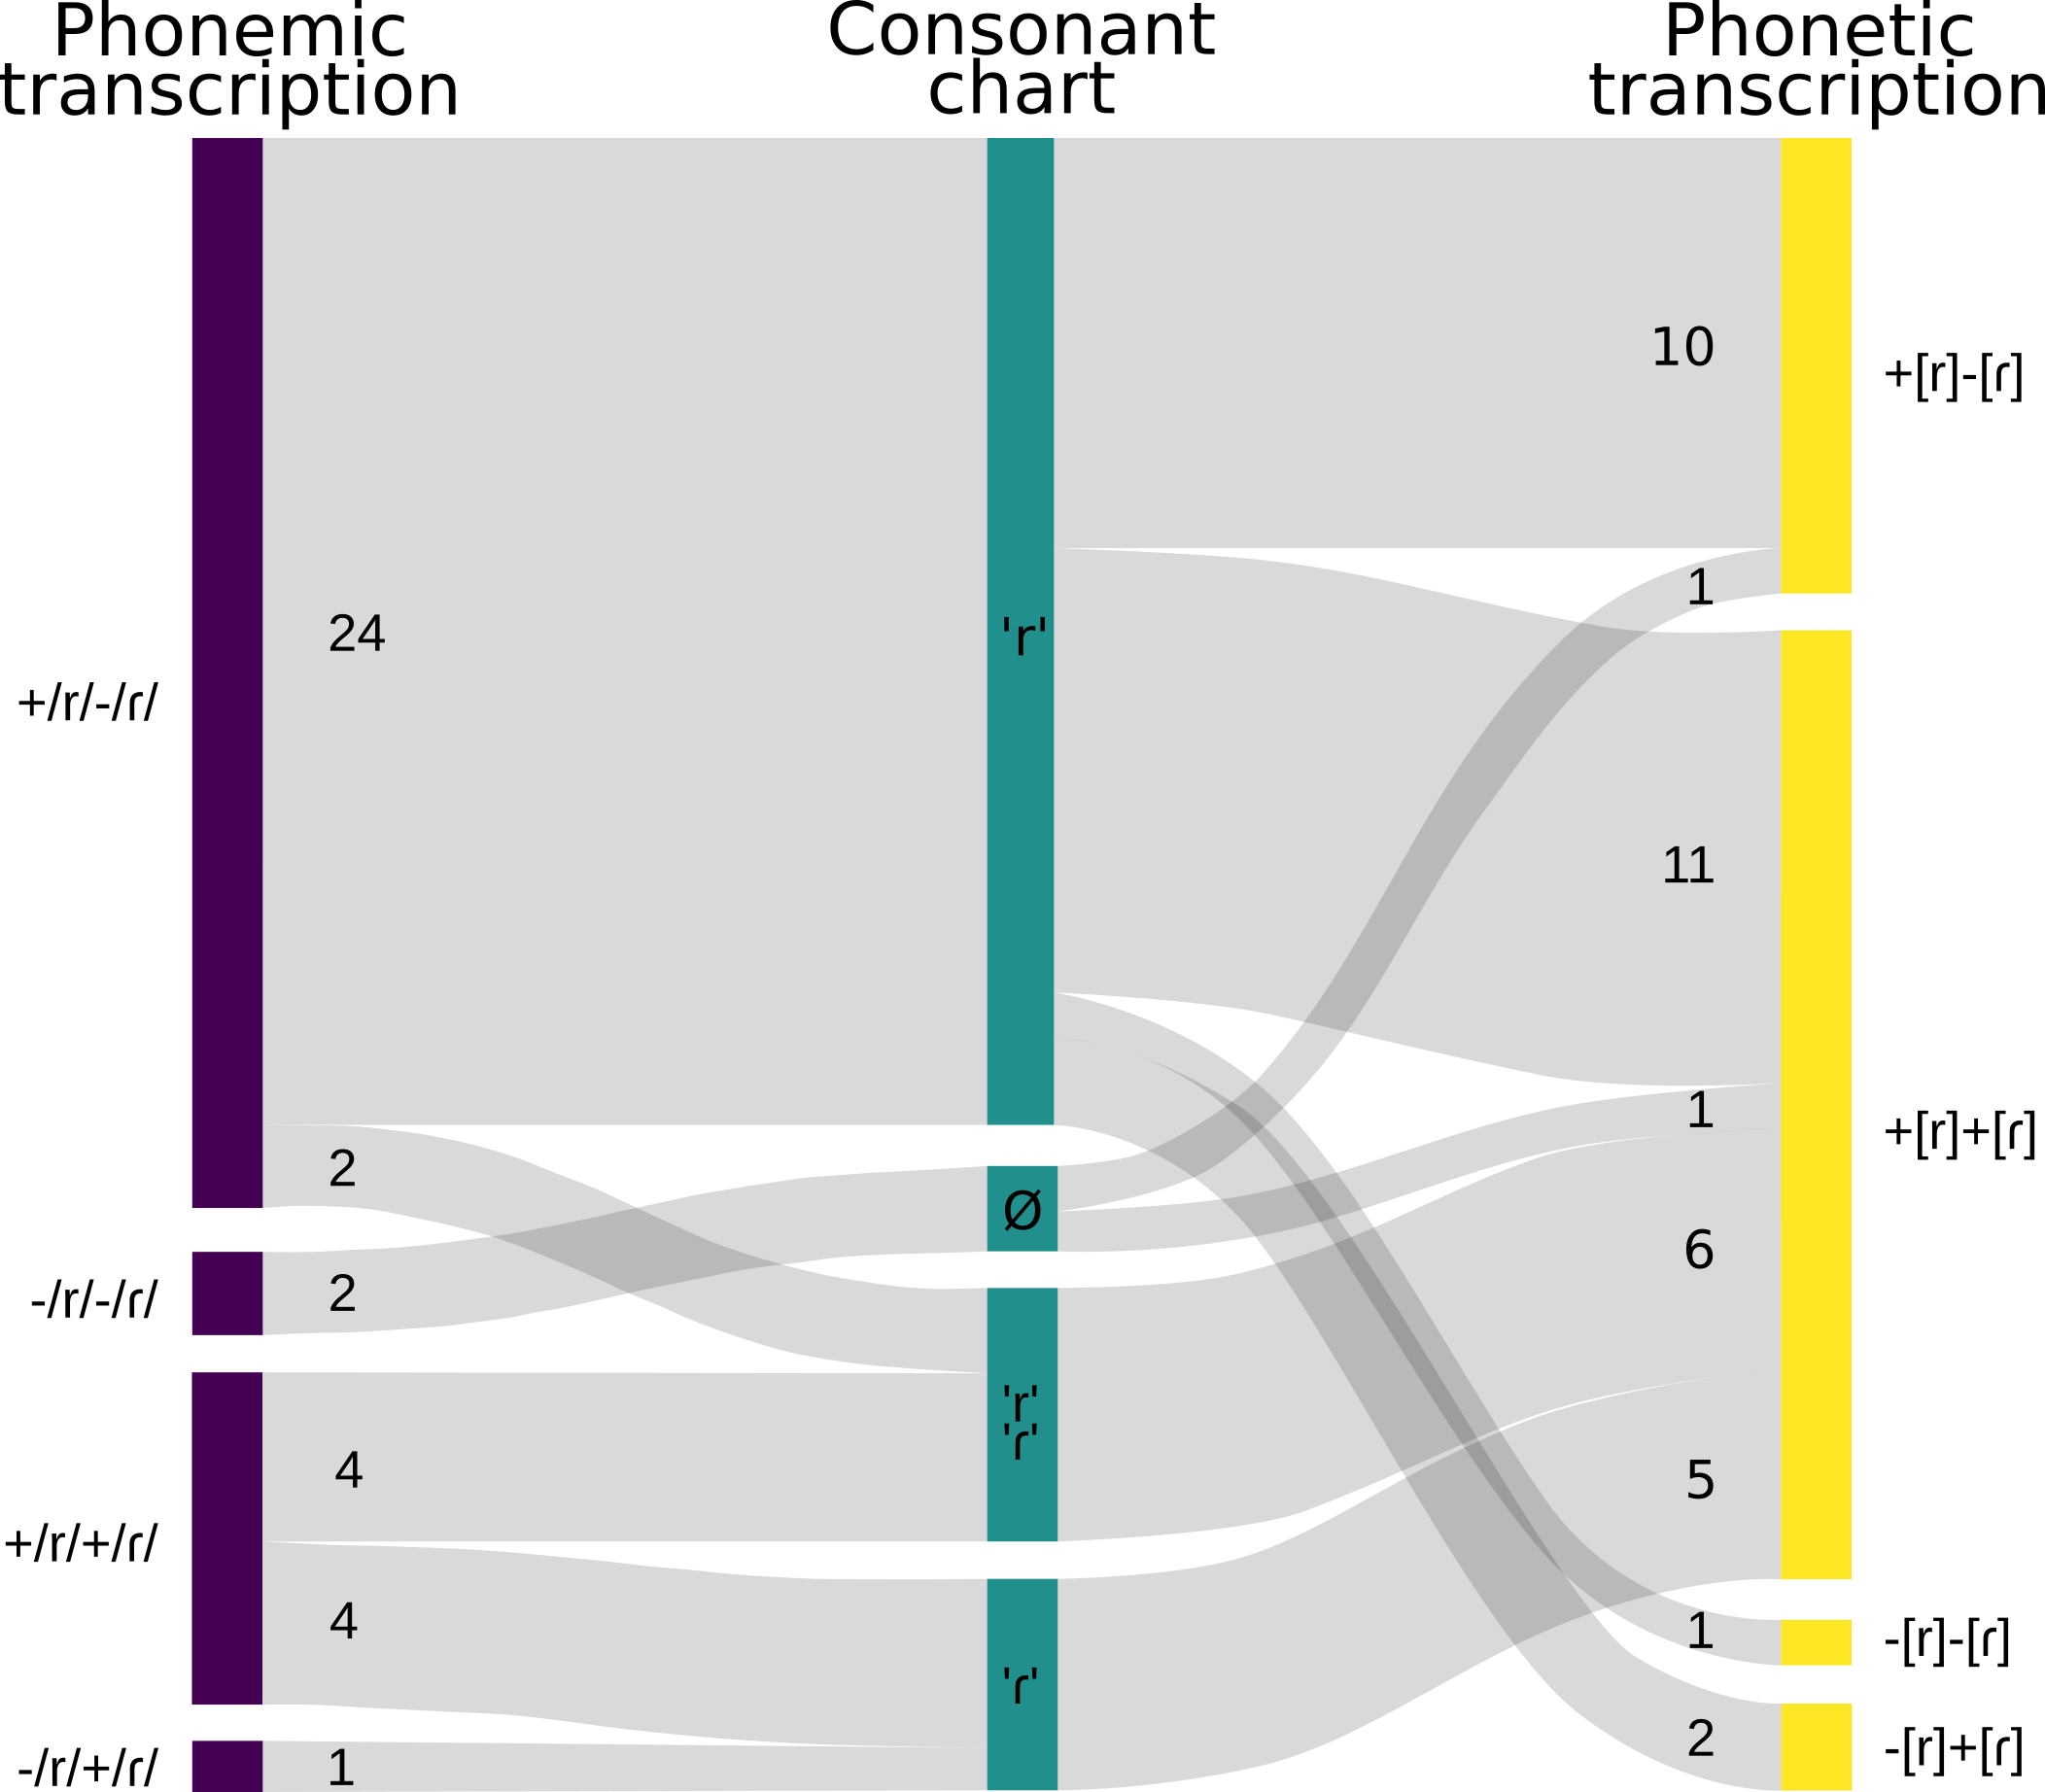
\includegraphics[width=0.75\linewidth]{jipa/images/sankey_phonemic_phonetic}
	\caption[Counts of illustrations with both phonemic and phonetic transcriptions when there is at least one \textit{r} in the illustration]{Counts of illustrations with both phonemic and phonetic transcriptions when there is at least one \textit{r} in the illustration, focusing on the phonemic transcription (left), the consonant chart (middle) and the phonetic transcription (right). The plus symbol (+) means the presence of \textit{r} in the narrative transcriptions and minus symbol (-) indicates its absence.}
	\label{fig:sankeyphonemicphonetic}
\end{figure}

We show a summary of these 37 illustrations in \autoref{fig:sankeyphonemicphonetic}. There are some interesting asymmetries between the use of \textit{r} in the phonetic and the phonemic transcriptions. For example, 24 illustrations contain an /r/ but do not contain an /ɾ/ in their phonemic transcription (left). All of these 24 illustrations include an \textit{r} in their consonant chart (left → middle). 10 of these 24 illustrations have a [r] but no [ɾ] in their phonetic transcription, 11 illustrations have a [r] and a [ɾ] in their phonetic transcription, one that in its phonetic transcription does not have any [r] or [ɾ], and two that have no [r] but only [ɾ] (middle → right). Also, there are two illustrations where both segments (trill and tap) are absent from the consonant chart (left → middle): in both cases, the phonemic transcriptions do not contain the segments, but the phonetic transcription for one illustration contains a [r] and for the other illustration it contains both segments [r] and [ɾ].\\

As shown in \autoref{fig:sankeyphonemicphonetic}, some authors do not always mention the \textit{r} in the consonant chart but do use the symbol in one of the transcriptions. In other cases, the use of \textit{r} in a phonemic transcription can be associated with a [r], with a [ɾ], with both, or even with none of these two segments. These results show that the presence of a [r] cannot be directly associated with a /r/ phoneme, in some cases the phonetic trill being associated with a /r/ but also with a /ɾ/, with both segments or even with none.

\newgeometry{inner=3.81cm,outer=3.81cm}

\begin{landscape}
\begin{longtable}{>{\raggedright\arraybackslash}m{4.5cm}cccc>{\centering\arraybackslash}m{2.5cm}>{\raggedright\arraybackslash}m{8cm}}
	%\resizebox{\textwidth}{!}{
	
%\begin{tabular}{>{\raggedright\arraybackslash}m{3.5cm}cccc>{\centering\arraybackslash}m{1.5cm}>{\raggedright\arraybackslash}m{3cm}}
	\\ \hline
	Title & [r] & /r/ & [ɾ] & /ɾ/ & Phonemic rhotic total & All phonetic segments \\
	\hline
	Afrikaans & 36 & 37 & 0 & 0 & 37 & 1 omission, 36 r \\
	\hline
	Amarasi & 2 & 5 & 3 & 0 & 5 & 3 ɾ, 2 r \\
	\hline
	\cellcolor{pink!40}Argentine Spanish & \cellcolor{pink!40}3 & \cellcolor{pink!40}3 & \cellcolor{pink!40}31 & \cellcolor{pink!40}31 & \cellcolor{pink!40}34 & \cellcolor{pink!40}31 ɾ, 3 r \\
	\hline
	Australian English & 0 & 11 & 3 & 0 & 11 & 11 ɹ, 3 ɾ as allophone of /t/ \\
	\hline
	\cellcolor{pink!40}Belarusian & \cellcolor{pink!40}16 & \cellcolor{pink!40}16 & \cellcolor{pink!40}0 & \cellcolor{pink!40}0 & \cellcolor{pink!40}16 & \cellcolor{pink!40}16 r \\
	\hline
	British English: Received Pronunciation & 0 & 11 & 0 & 0 & 11 & 11 ɹ \\
	\hline
	Brunei Malay & 3 & 19 & 12 & 0 & 19 & 12 ɾ, 3 ɹ, 1 omission, 3 r \\
	\hline
	Cagliari Sardinian & 23 & 27 & 16 & 0 & 27 & 16 ɾ (of which 12 are allophones of /t d/), 23 r \\
	\hline
	Castilian Spanish & 2 & 36 & 34 & 0 & 36 & 34 ɾ, 2 r \\
	\hline
	\cellcolor{gray!20}Central Arrernte & \cellcolor{gray!20}1 & \cellcolor{gray!20}0 & \cellcolor{gray!20}21 & \cellcolor{gray!20}22 & \cellcolor{gray!20}22 & \cellcolor{gray!20}21 ɾ, 1 r (we did not include ɻ) \\
	\hline
	Eastern Andalusian Spanish & 3 & 12 & 28 & 22 & 34 & 28 ɾ, 3 omissions, 3 r \\
	\hline
	Gayo & 8 & 26 & 18 & 0 & 26 & 18 ɾ, 8 r \\
	\hline
	\cellcolor{pink!40}Goizueta Basque & \cellcolor{pink!40}15 & \cellcolor{pink!40}15 & \cellcolor{pink!40}13 & \cellcolor{pink!40}13 & \cellcolor{pink!40}28 & \cellcolor{pink!40}13 ɾ, 15 r \\
	\hline
	Greek Thrace Xoraxane Romane & 8 & 18 & 11 & 2 & 20 & 11 ɾ, 1 omission, 8 r \\
	\hline
	\cellcolor{gray!20}Indonesian Bajau (East Lombok)
	& \cellcolor{gray!20}2 & \cellcolor{gray!20}1 & \cellcolor{gray!20}29 & \cellcolor{gray!20}40 & \cellcolor{gray!20}41 & \cellcolor{gray!20}39 ɾ, 2 r \\
	\hline
	Italian & 15 & 28 & 11 & 0 & 28 & 11 ɾ, 1 ɹ, 1 t̚, 15 r (there is one ɹɾ included in the count of taps here and there are 5 rː) \\
	\hline
	\cellcolor{gray!20}Itunyoso Trique & \cellcolor{gray!20}4 & \cellcolor{gray!20}2 & \cellcolor{gray!20}5 & \cellcolor{gray!20}8 & \cellcolor{gray!20}10 & \cellcolor{gray!20}5 ɾ, 1 ɽ, 4 r \\
	\hline
%\end{tabular}}
%\begin{tabular}{>{\raggedright\arraybackslash}m{3.5cm}cccc>{\centering\arraybackslash}m{1.5cm}>{\raggedright\arraybackslash}m{3cm}}
%\hline
	\cellcolor{pink!40}Kalabari-ljo & \cellcolor{pink!40}50 & \cellcolor{pink!40}50 & \cellcolor{pink!40}0 & \cellcolor{pink!40}0 & \cellcolor{pink!40}50 & \cellcolor{pink!40}50 r \\

	Kazakh & 6 & 15 & 9 & 0 & 15 & 9 ɾ, 6 r \\
	\hline
	Liverpool English & 3 & 10 & 1 & 0 & 11 & 1 ɾ, 7 ɹ, 3 r \\
	\hline
	\cellcolor{pink!40}Mavea & \cellcolor{pink!40}36 & \cellcolor{pink!40}36 & \cellcolor{pink!40}0 & \cellcolor{pink!40}0 & \cellcolor{pink!40}36 & \cellcolor{pink!40}36 r \\
	\hline
	\cellcolor{pink!40}Notes on the phonetics of Latvian & \cellcolor{pink!40}19 & \cellcolor{pink!40}19 & \cellcolor{pink!40}0 & \cellcolor{pink!40}0 & \cellcolor{pink!40}19 & \cellcolor{pink!40}19 r \\
	\hline
	\cellcolor{gray!20}Philippine English (Metro Manila acrolect) & \cellcolor{gray!20}1 & \cellcolor{gray!20}0 & \cellcolor{gray!20}0 & \cellcolor{gray!20}0 & \cellcolor{gray!20}30 & \cellcolor{gray!20}18 ɹ, 11 ɝ, 1 r \\
	\hline
	Russian & 17 & 20 & 3 & 0 & 20 & 3 ɾ, 17 r \\
	\hline
	Sasak, Meno-Mené dialect & 0 & 10 & 9 & 0 & 10 & 9 ɾ, 1 omission \\
	\hline
	Saterland Frisian & 9 & 23 & 2 & 0 & 23 & 2 ɾ (but allophone of /t/), 3 omissions, 1 ɹ, 10 vowels, 9 r \\
	\hline
	\cellcolor{gray!20}Seenku & \cellcolor{gray!20}1 & \cellcolor{gray!20}0 & \cellcolor{gray!20}3 & \cellcolor{gray!20}0 & \cellcolor{gray!20}4 & \cellcolor{gray!20}3 ɾ, 1 r \\
	\hline
	\cellcolor{gray!20}Standard Georgian & \cellcolor{gray!20}10 & \cellcolor{gray!20}9 & \cellcolor{gray!20}23 & \cellcolor{gray!20}30 & \cellcolor{gray!20}39 & \cellcolor{gray!20}23 ɾ, 4 tʂ, 1 ɚ, 1 omission, 10 r \\
	\hline
	Standard Malay (Brunei) & 6 & 28 & 22 & 0 & 28 & 22 ɾ, 6 r \\
	\hline
	\cellcolor{pink!40}Tamambo & \cellcolor{pink!40}19 & \cellcolor{pink!40}19 & \cellcolor{pink!40}0 & \cellcolor{pink!40}0 & \cellcolor{pink!40}19 & \cellcolor{pink!40}19 r \\
	\hline
	\cellcolor{pink!40}Tashlhiyt Berber & \cellcolor{pink!40}18 & \cellcolor{pink!40}18 & \cellcolor{pink!40}0 & \cellcolor{pink!40}0 & \cellcolor{pink!40}18 & \cellcolor{pink!40}18 r \\
	\hline
	\cellcolor{pink!40}Trapezountian Pontic Greek in Etoloakarnania & \cellcolor{pink!40}2 & \cellcolor{pink!40}2 & \cellcolor{pink!40}20 & \cellcolor{pink!40}20 & \cellcolor{pink!40}22 & \cellcolor{pink!40}20 ɾ, 2 r \\
	\hline
	The dialect of Venice & 23 & 38 & 15 & 0 & 38 & 15 ɾ, 23 r \\
	\hline
	The Flemish-Brabant dialect of Orsmaal-Gussenhoven & 21 & 32 & 8 & 0 & 32 & 8 ɾ (of which one is ɾɹ), 3 omissions, 21 r \\
	\hline
	\cellcolor{pink!40}'The North Wind and the Sun' in the Breton of the Isle of Groix & \cellcolor{pink!40}26 & \cellcolor{pink!40}26 & \cellcolor{pink!40}0 & \cellcolor{pink!40}0 & \cellcolor{pink!40}26 & \cellcolor{pink!40}26 r \\
	\hline
	\cellcolor{pink!40}Ukrainian & \cellcolor{pink!40}21 & \cellcolor{pink!40}21 & \cellcolor{pink!40}0 & \cellcolor{pink!40}0 & \cellcolor{pink!40}21 & \cellcolor{pink!40}21 r \\
	\hline
	Zurich German & 19 & 21 & 0 & 0 & 21 & 2 ʁ, 19 r \\
	\hline
%\end{tabular}

%^}
	\caption[Comparison of counts of \textit{r} and \textit{ɾ} in illustrations with a phonetic and phonemic transcription]{Comparison of counts of \textit{r} and \textit{ɾ} in illustrations with a phonetic and phonemic transcription, with all the possible phonetic segments that can be associated with a phonemic rhotic segment (including instances where there is a rhotic in the phonemic transcription but no equivalent rhotic in the phonetic transcription) or that are \textit{r}-like segment (allophones of plosives). Unshaded rows correspond to illustrations where [r] is less frequent than /r/, gray rows correspond to illustrations where [r] is more frequent than /r/, and red lines correspond to illustrations where [r] is as frequent as /r/.}
	\label{tab:tablecompaphonophone}
\end{longtable}
\end{landscape}

\restoregeometry

We use the varieties of English as an example of how the use of the symbol \textit{r} instead of the symbol \textit{ɹ} for the alveolar approximant is driven by simplicity of use and not by phonetic or phonological reasons. This is clearly the case for Australian English and British English Received Pronunciation, where \textit{r} is found in the phonemic transcription while [ɹ] is the main allophone found in the phonetic transcription. Things are more complicated for Liverpool English, where [r], [ɾ] and [ɹ] are used in the phonetic transcription while the author only mentions [ɾ] and [ɹ] as allophones, leading to difficulties in interpreting the symbol \textit{r} since it is not specified in the illustration as a possible allophone of /r/. \\

The use of the symbol \textit{r} is not necessarily transparent in phonetic transcriptions. The symbol \textit{r} is found for Zurich German but its interpretation is made difficult by the fact that while /r/ may have alveolar and uvular allophones, [r] is not specified as one of them. It is therefore not possible to say with certainty which allophone has been represented. \\

The use of \textit{r} does not necessarily imply the occurrence of [r] in phonetic transcriptions. The Sasak, Meno–Mené dialect illustration uses the symbol \textit{r} for the phoneme in the phonemic transcription, but the symbol is absent from the phonetic transcription. The authors do specify that ‘/r/ is sometimes produced as an alveolar tap’ \parencite[97]{archangeliSasakMenoMeneDialect2020} while an actual trilled realization occurs in word initial and word final positions. All occurrences of /r/ in the transcription appear in intervocalic positions and are realized as [ɾ], with one occurrence of /r/ in a pre–nasal context being omitted. [ɾ] seems to be a common realization of /r/ when the latter has more than one allophone in the phonetic transcription.\\

In \autoref{tab:tablecompaphonophone}, the non–colored (i.e., white background) rows represent the illustrations where the number of \textit{r} tokens is lower in the phonetic transcription than in the phonemic one. The last column indicates how the segments are realized and hence highlights the variation in the realizations of the rhotics that the authors reported. The grayed rows in \autoref{tab:tablecompaphonophone} highlight the cases where in there are more \textit{r} in the phonetic transcription than in the phonemic one: except for Itunyoso Trique (where there is a difference of two more occurrences of [r]), for the rest of the illustrations the difference consists of one more [r].\\

Finally, it is important to highlight the red rows in \autoref{tab:tablecompaphonophone} (11 illustrations) which denote when the same number of \textit{r} tokens is present in both transcriptions. This can be interpreted either as there being no explicitly reported variation among rhotics in these illustrations, or that all the trills in the phonemic transcription are realized as phonetic trills. In three of these cases, there is a contrast between /ɾ/ and /r/, and in eight cases (including the three cases aforementioned), the transcription is said to be ‘narrow’, ‘semi–narrow’ or ‘detailed’, supporting our second hypothesis that /r/ are realized as [r]. For example, in Kalabari–Ilo, there are 50 tokens of /r/ in the phonemic transcription, realized as 50 tokens of [r] in the narrow transcription also provided. As allophones other than the trill are mentioned, we infer that all tokens of /r/ are trilled.

\paragraph{Illustrations with phonetic transcriptions only}

\begin{figure}
	\centering
	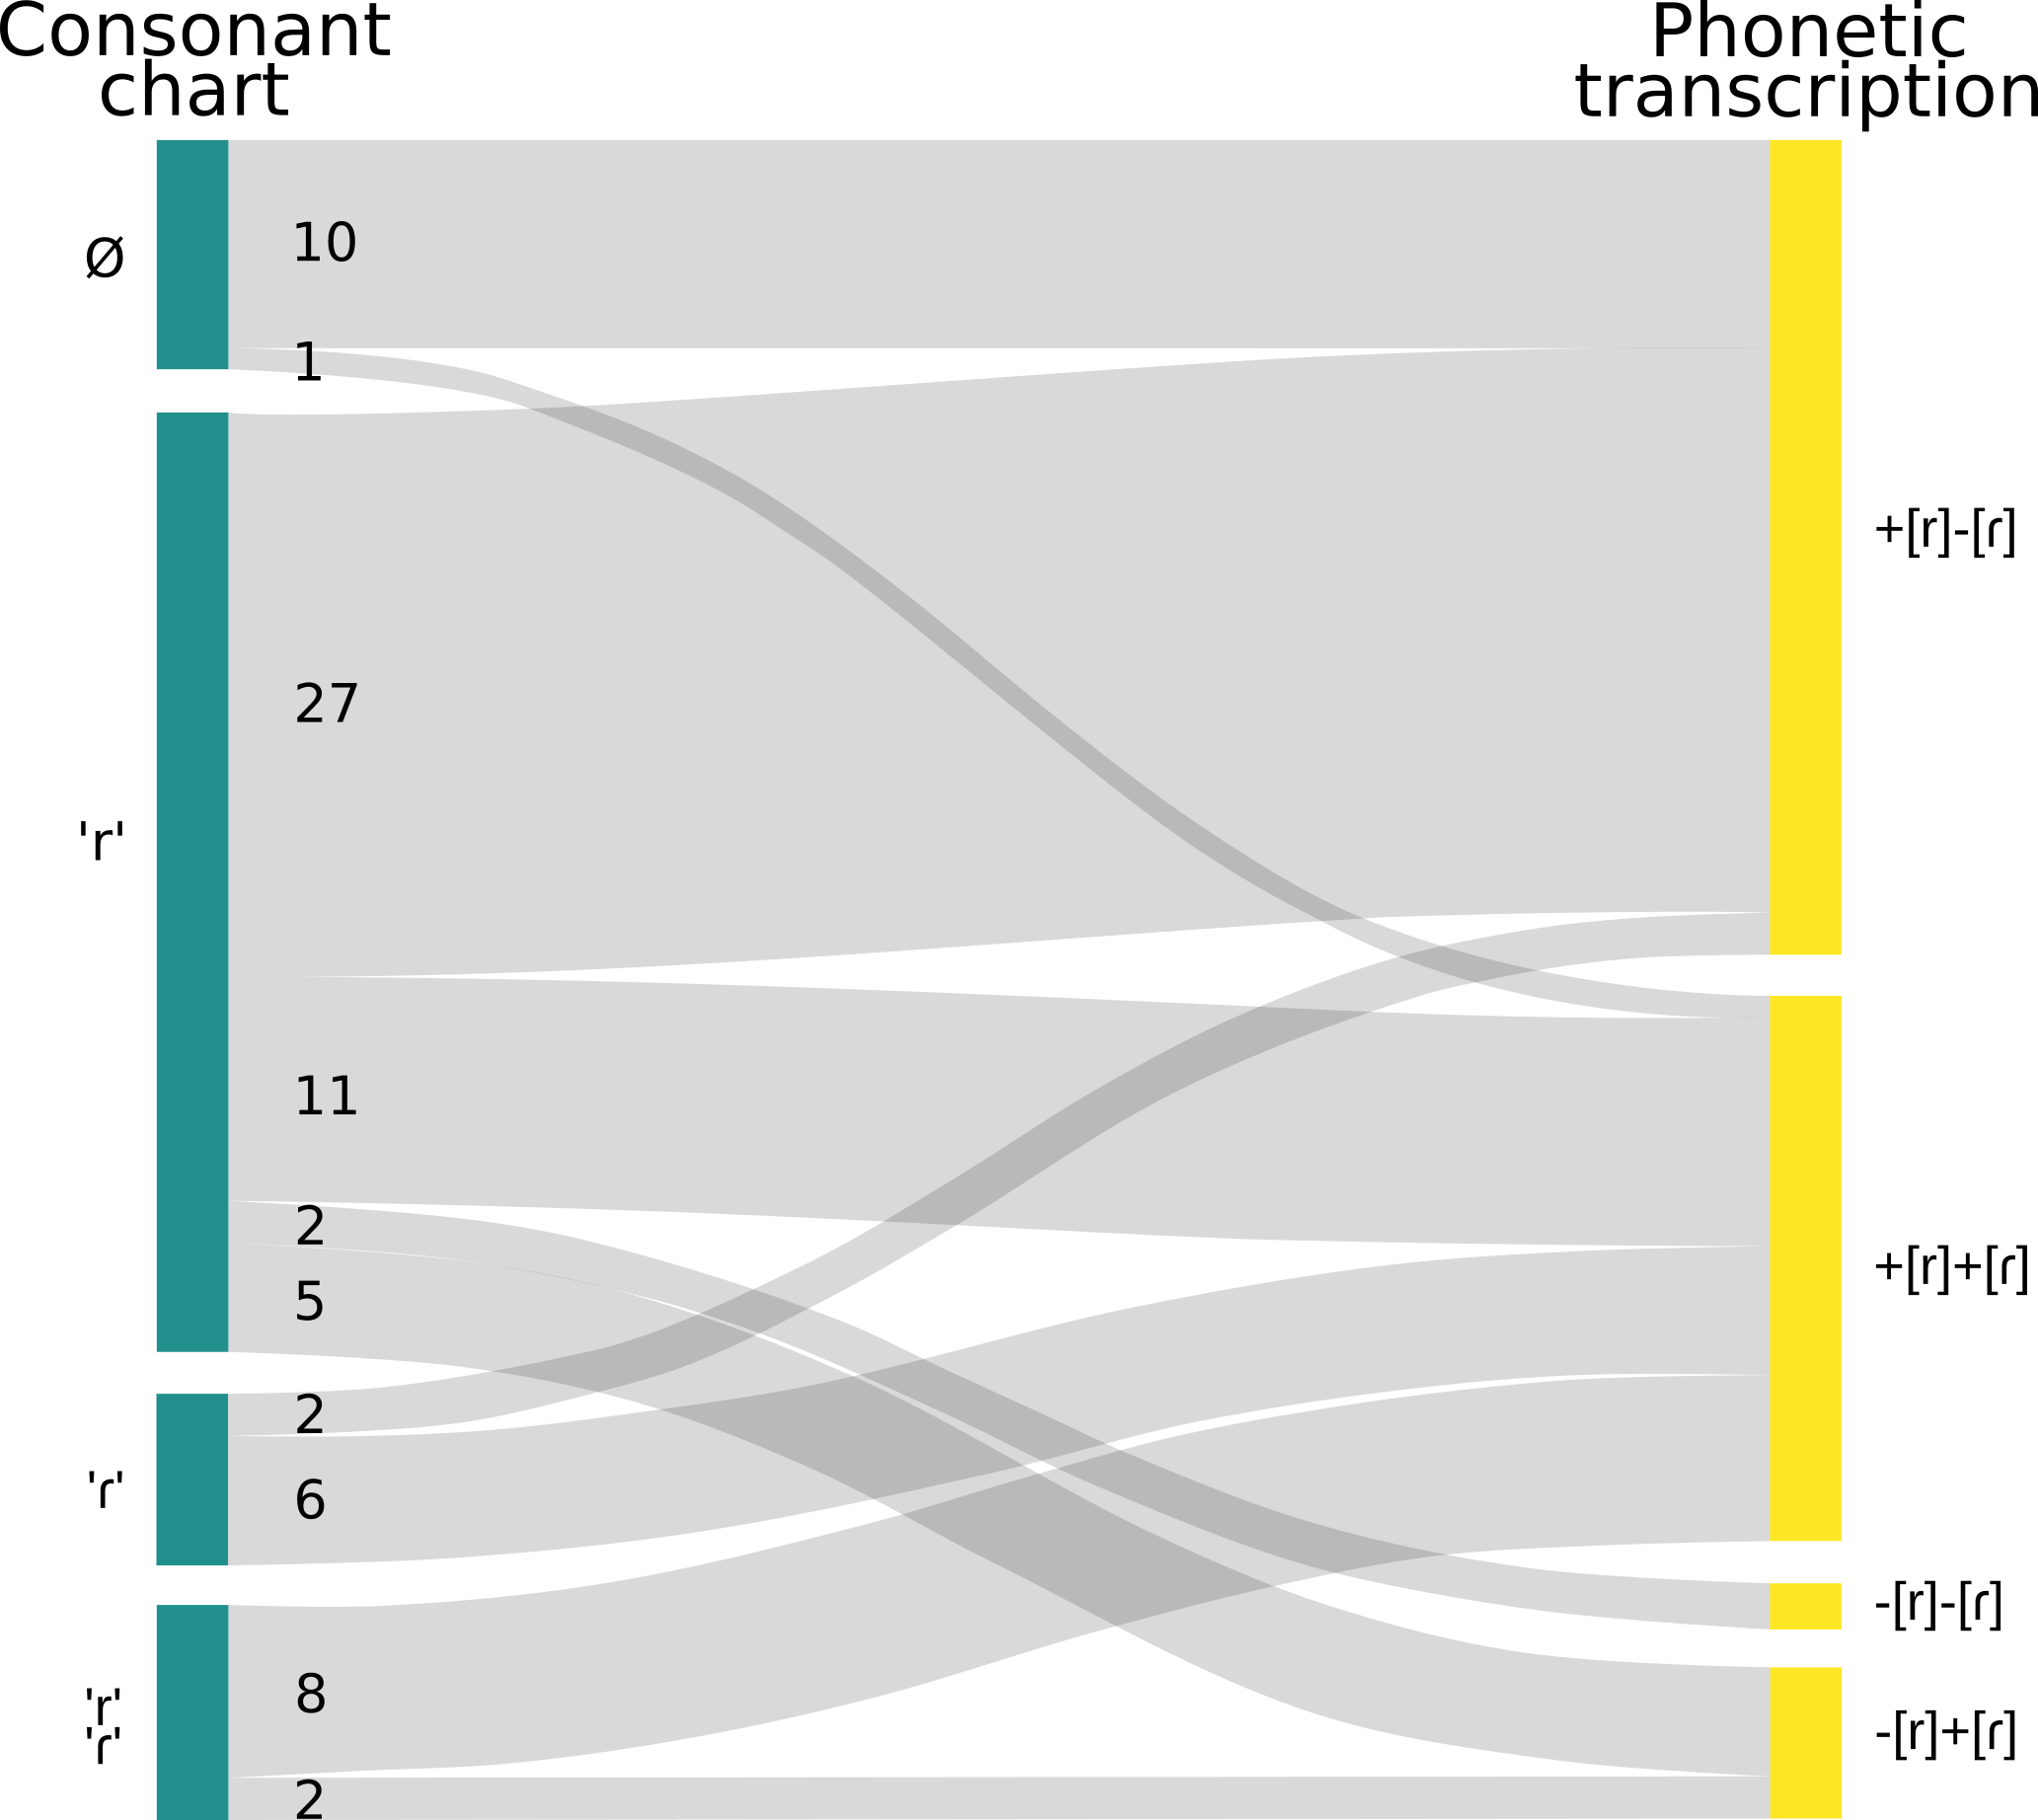
\includegraphics[width=0.75\linewidth]{jipa/images/sankey_phonetic}
	\caption[Counts of illustrations with a phonetic transcription only, which include at least one \textit{r} in the illustration]{Counts of illustrations with a phonetic transcription only, which include at least one \textit{r} in the illustration, focusing on the consonant chart (left) or on the phonetic transcription (right). The absence of \textit{r} in the consonant chart does not obligatorily imply that there will not be any [r] in the phonetic transcription, nor does the presence of \textit{r} obligatorily imply the presence of [r] in the phonetic transcription.}
	\label{fig:sankeyphonetic}
\end{figure}

Illustrations containing only an \textit{r} in their consonant chart have different types of possible production (\autoref{fig:sankeyphonetic}). We found illustrations where only [r] is present in the transcription (27 illustrations). In this first case, based on the author's transcription, we can consider that speakers are trilling for all the instances of their ‘r’. The second case corresponds to cases where there both [ɾ] and [r] are present (11 illustrations), both phones expected to be allophones of a /r/. The third case corresponds to the few illustrations which contain only [ɾ] in their transcription when a r was presented in the chart (five illustrations), and we finally find two illustrations where there is neither [r] nor [ɾ] in the transcription although the segment was present in the consonant table. Regarding the 10 illustrations where both  \textit{r} and \textit{ɾ} are present in the consonant chart, there is no [r] in the transcription for two of them while both phones [r] and  [ɾ] are found for the other eight.

\paragraph{Illustrations with a phonemic transcription only}

\begin{figure}
	\centering
	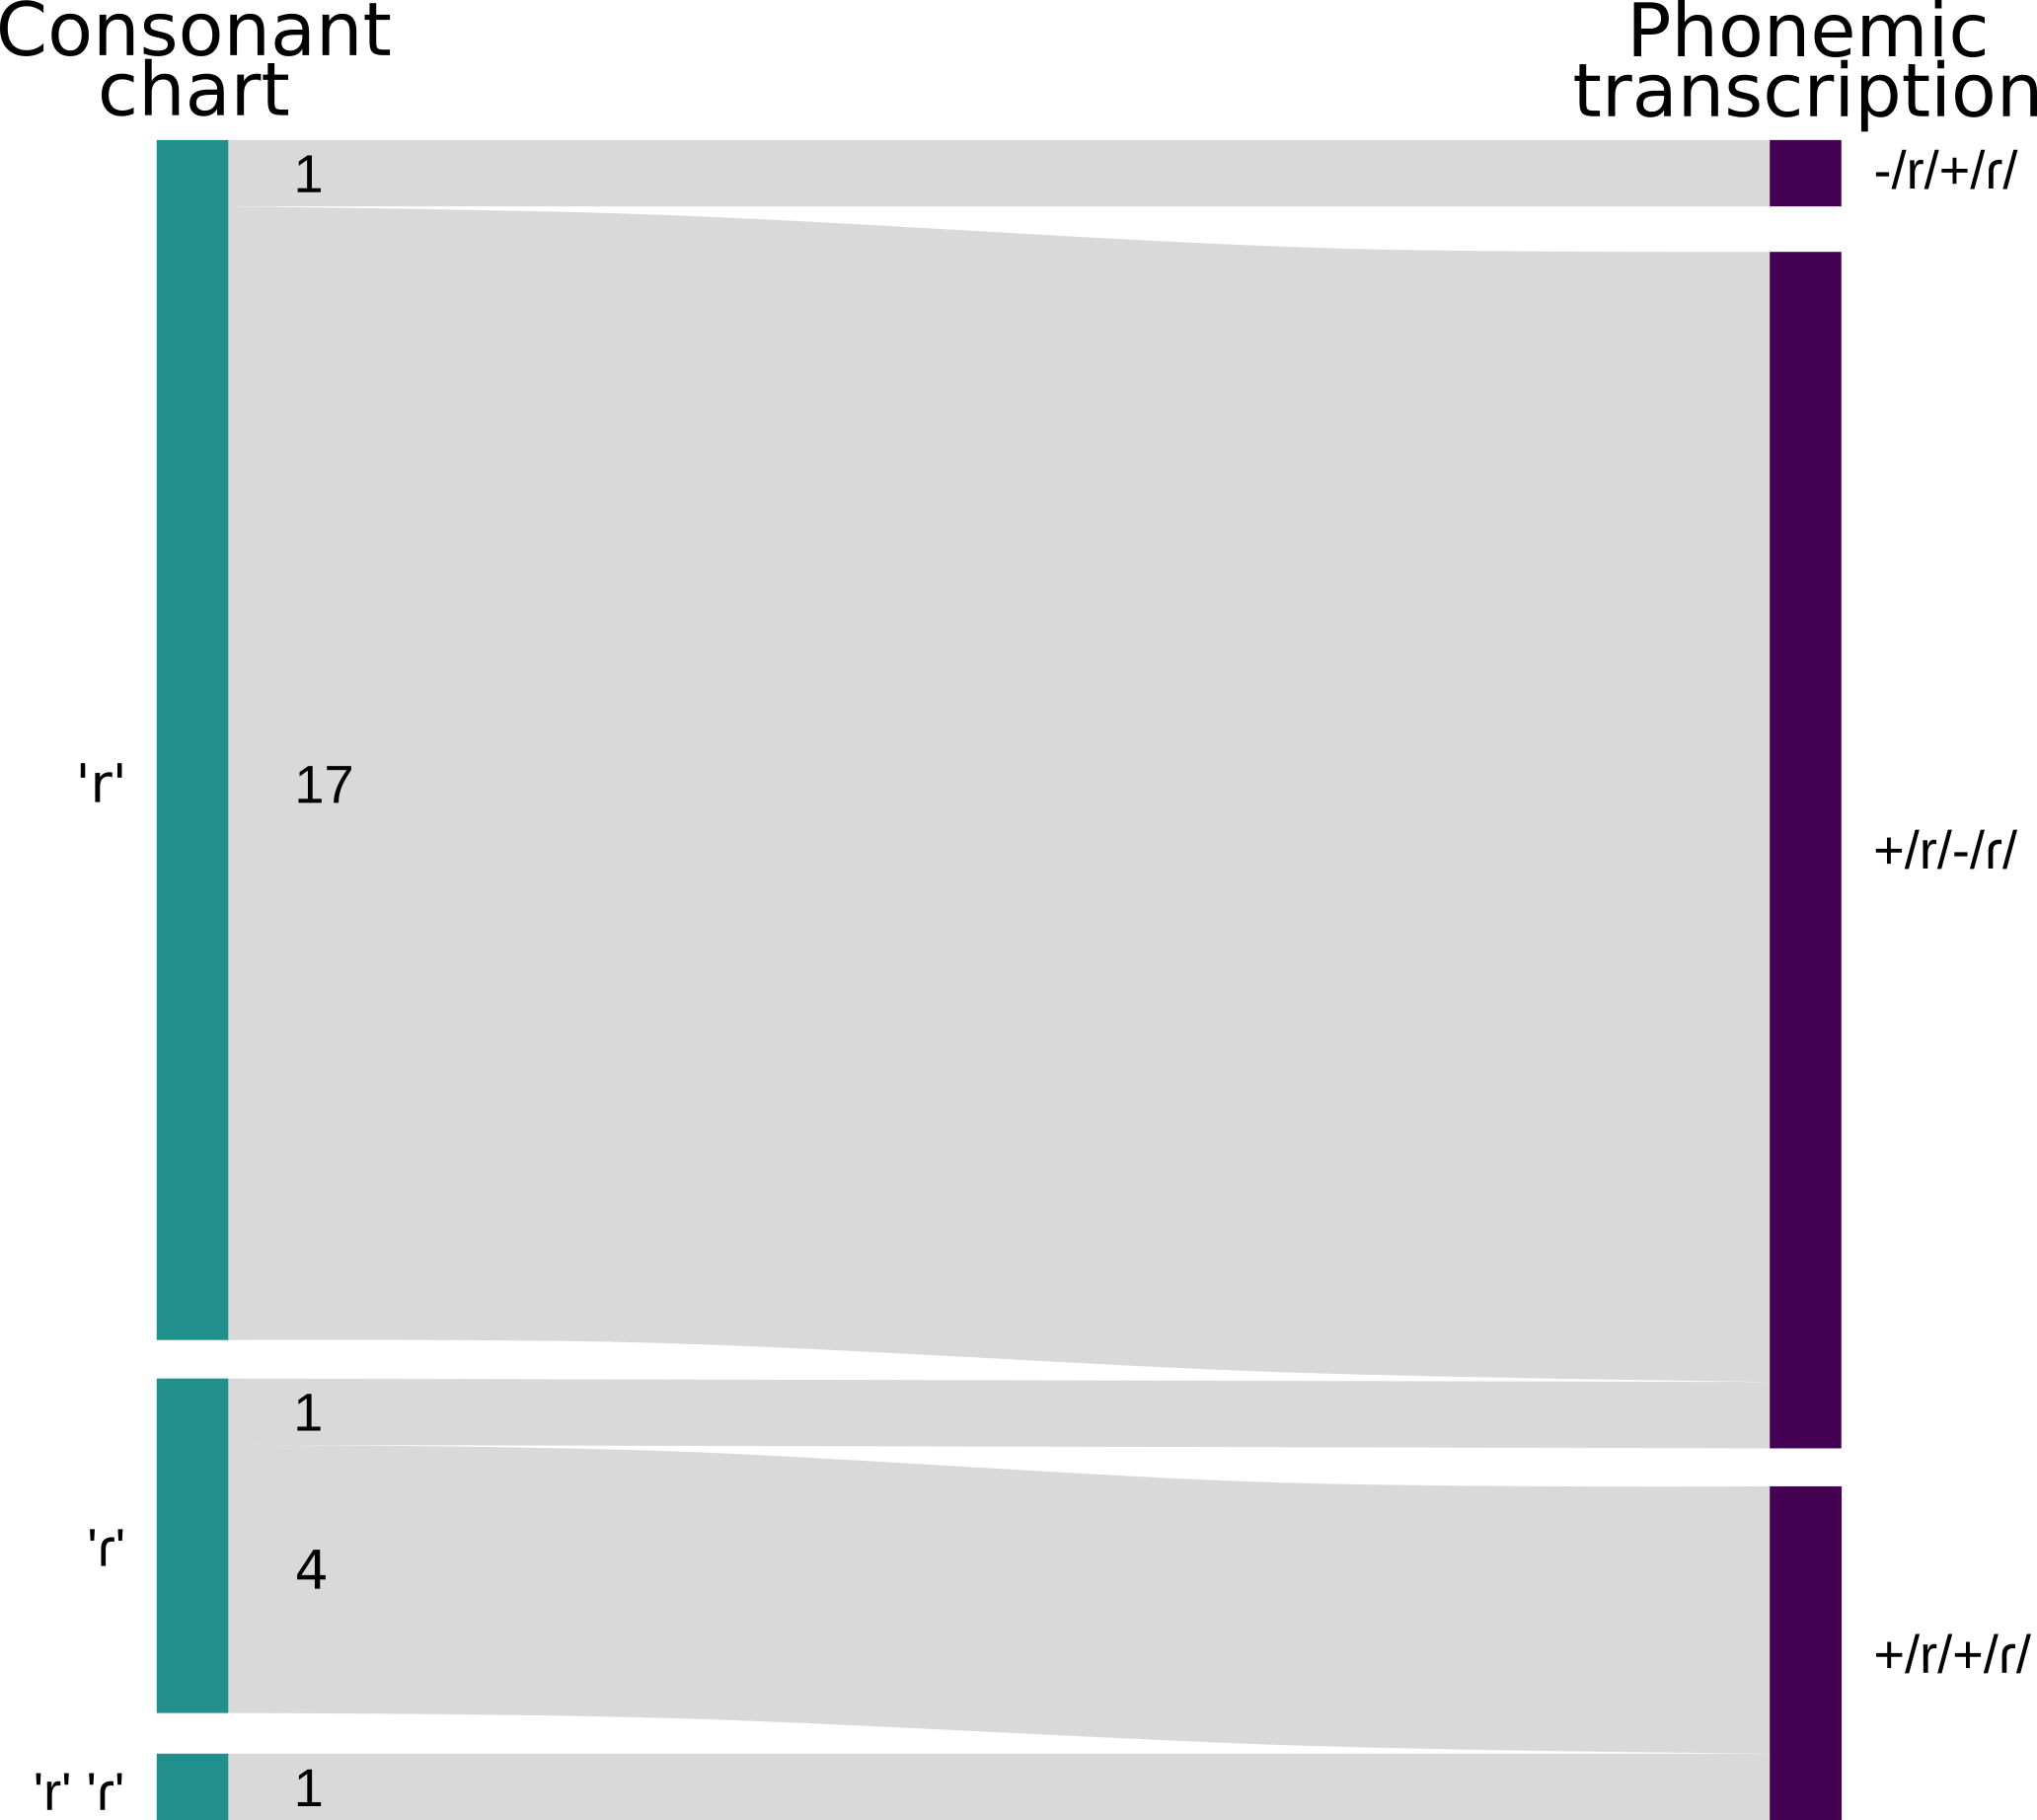
\includegraphics[width=0.75\linewidth]{jipa/images/sankey_phonemic}
	\caption[Counts of illustrations with a phonemic transcription only, which include at least one r in the illustration]{Counts of illustrations with a phonemic transcription only, which include at least one r in the illustration, focusing on the consonant chart (left) or on the phonemic transcription (right).}
	\label{fig:sankeyphonemic}
\end{figure}

Finally, it is important to also take into account the illustrations that are grouped in our third category, where we find only a phonemic transcription (\autoref{fig:sankeyphonemic}). Although their transcriptions refer to a level more abstract from the phonetic reality of the speaker’s production, one can still see differences between what is expected from the consonant chart and the symbols that are present in the transcription. In all the illustrations of this category except one, there is at least one /r/ in the phonemic transcription. In the remaining illustration, /r/ is absent from the phonemic transcription while /ɾ/ is present, in contrast with the consonant chart where there is only \textit{r} and not \textit{ɾ}.

\subsubsection{‘\textit{r}–like’ sound frequencies}

We then looked at the full transcriptions of the illustrations where there was at least one \textit{r}, in order to get at a first approximation of their frequency while taking all rhotic segments (i.e., all allophones of a rhotic phoneme) into account. Since the total number of segments and the number of rhotics differs across the illustrations, it is important to consider these in order to be able to meaningfully compare the frequency of \textit{r} among them.

\paragraph{Overall rhoticity}

The overall rhoticity, defined as freq$_\textrm{rhot}$ = n$_\textrm{ʀ}$ / n$_\textrm{seg}$, was computed based on all the possible segments that could be considered as rhotics in the transcription. Critical analysis of ambiguous segments (like the \textit{ɾ} which can be and allophone of a plosive, or \textit{ʁ} that can behave like a fricative but not like a rhotic) was done on the basis of the full illustration, so as to only select those segments that can be considered rhotics. For languages with two or more contrastive rhotics, this measure conflates all rhotic phonemes — it does not contain information on the relative frequencies of each rhotic phoneme individually.\\

\begin{figure}
	\centering
	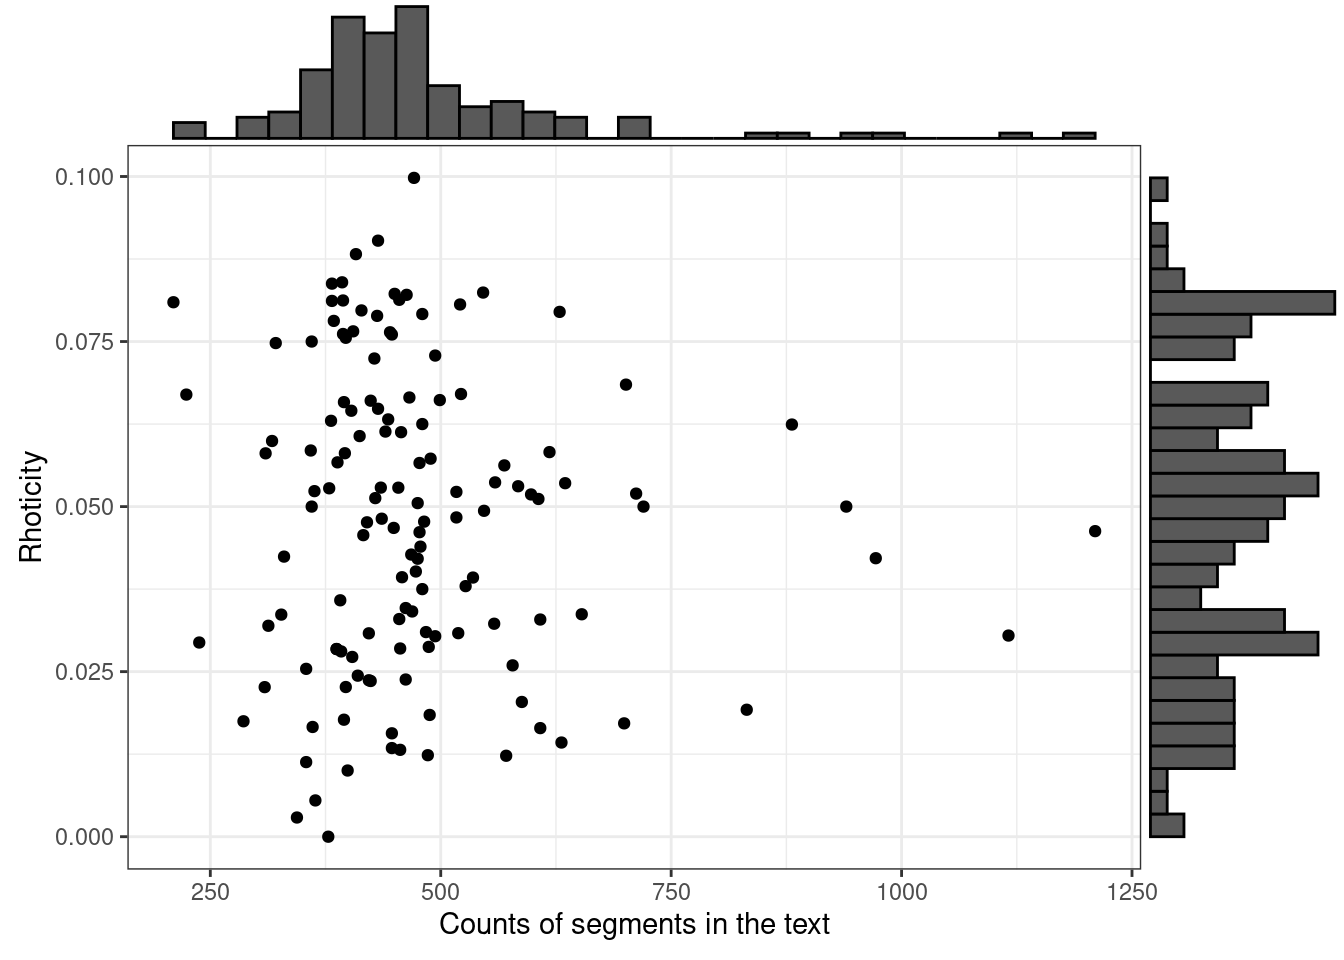
\includegraphics[width=0.75\linewidth]{jipa/images/rhoticy_freq}
	\caption[Rhoticity for the 135 transcriptions as a function of the number of segments in the written transcription]{Rhoticity for the 135 transcriptions on the vertical axis (1 illustration does not have any transcription and was removed) as a function of the number of segments in the written transcription on the horizontal axis.}
	\label{fig:rhoticyfreq}
\end{figure}

Unsurprisingly, \autoref{fig:rhoticyfreq} illustrates that not all transcriptions have the same length (minimum 210, mean 477.5, median 449, sd 148.5, IQR 122.5 and maximum 1210 segments). By dividing by the number of segments we control for text length in order to have a normalized estimate of rhoticity. There is variation in the rhoticity, freq$_\textrm{rhot}$ (minimum 0.0, mean 0.048, median 0.05, standard deviation sd 0.023, interquartile range IQR 0.035, and maximum 0.1). Figure 9 shows that it is not because a transcription contains a lot of segments that its overall rhotic frequency is high. For example, the transcription of the illustration of Shipibo \parencite{valenzuelaShipibo2001} contains 1116 segments while its rhoticity is about 0.03, on the other side, the illustration of Standard Georgian \parencite{shostedStandardGeorgian2006} contains 432 segments but its rhoticity is about 0.09 (one of the highest). A rhoticity of 0.0 corresponds to cases where there was an \textit{r} in the illustration but there wasn’t any rhotic in the narrative, possibly due to its very low frequency. This measure of rhoticity can be compared with estimates of trill and tap frequencies reported below.

\paragraph{Trill frequency}

\begin{figure}
	\centering
	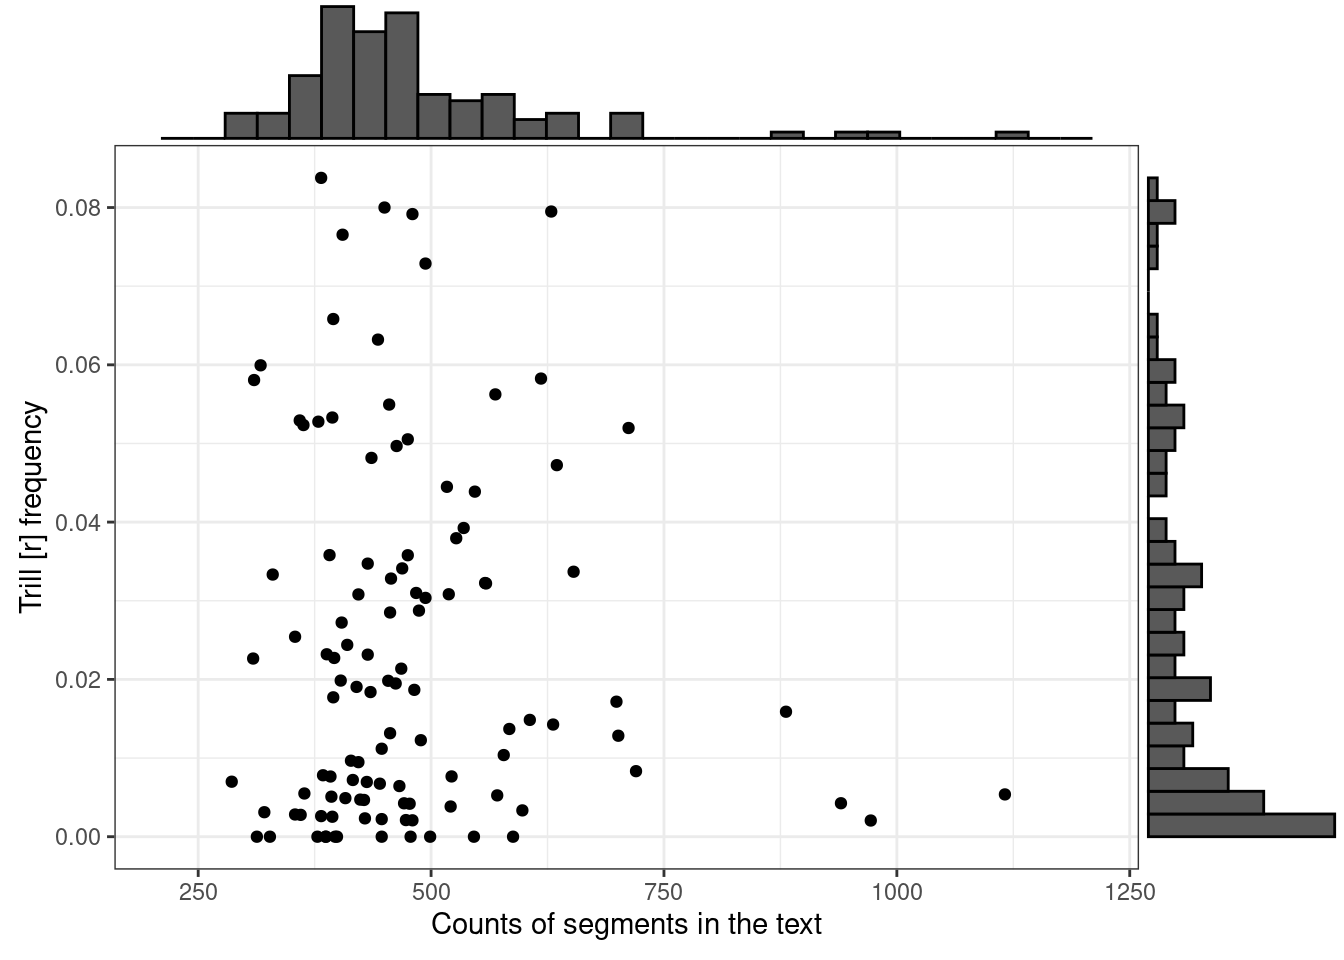
\includegraphics[width=0.75\linewidth]{jipa/images/trill_phonetic_freq}
	\caption[\textrm{[r]} frequency for the 111 transcriptions as a function of the number of segments in the written transcription]{[r] frequency (vertical axis) for the 111 transcriptions as a function of the number of segments in the written transcription (horizontal axis).}
	\label{fig:trillphoneticfreq}
\end{figure}

\autoref{fig:trillphoneticfreq} illustrates that the trill [r] frequency varies between a maximum of 0.084 (\textit{The dialect of Hasselt}) and a minimum of 0.0 (for 12 illustrations that do not contain [r] in their transcription), with a mean of 0.024, a median of 0.018 (both lower than for overall rhoticity), a standard deviation of 0.023, and an interquartile range of 0.031. A Wilcoxon test shows that the trill frequency is significantly lower than the mean of rhoticity 0.048 ($p<.0001$). This can be explained by the fact that in many cases the trill is not the only allophone used in the transcription to represent a rhotic segment (there are 43 illustrations where there is only one rhotic segment in the consonant chart, 28 where there are more than one rhotic segment in the consonant chart, and two illustrations where there is no rhotic segment in the consonant chart).


\begin{figure}
	\centering
	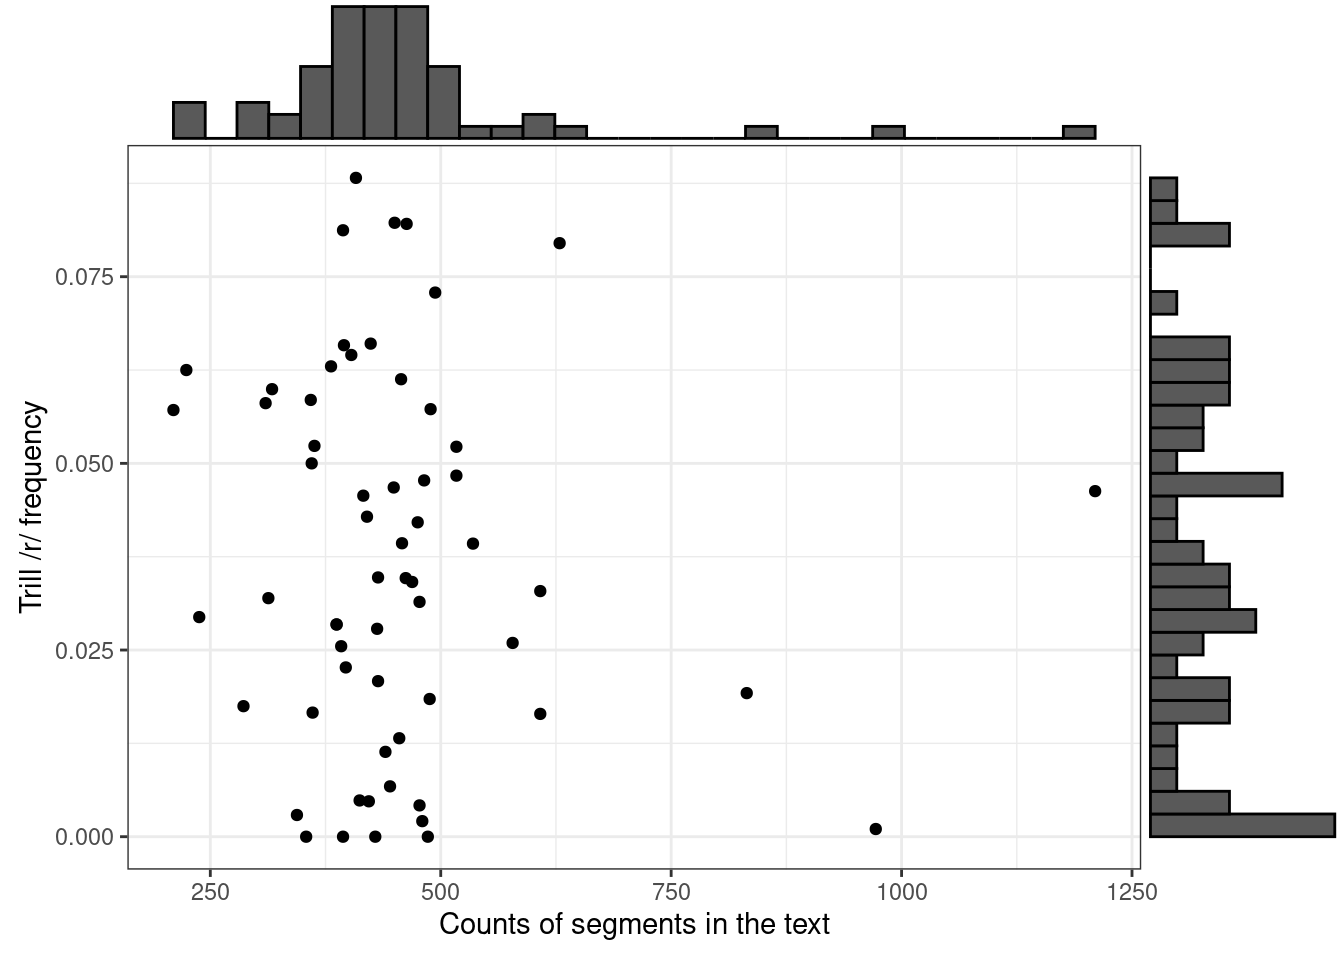
\includegraphics[width=0.75\linewidth]{jipa/images/trill_phonemic_freq}
	\caption[\textrm{/r/} frequency for the 61 transcriptions as a function of the number of segments in the written transcription]{/r/ frequency (vertical axis) for the 61 transcriptions as a function of the number of segments in the written transcription (horizontal axis).}
	\label{fig:trillphonemicfreq}
\end{figure}

\autoref{fig:trillphonemicfreq} illustrates that trill /r/ frequency varies between a maximum of 0.088 and a minimum of 0.0 (4 illustrations where there is no /r/ in the transcription of the narrative), with a mean of 0.037,  a median of 0.035 (both lower than for overall rhoticity), a standard deviation of 0.025, and an interquartile range of 0.04.\footnote{This maximum corresponds to Castilian Spanish, but it is important to mention that the broad transcription comes from Jones \& Dahl (1944: 16, mentioned by 	Martı́nez–Celdrán et al., 2003). The authors did not use the symbol \textit{ɾ} in opposition to \textit{r}, instead contrasted /r/ and /rr/ which are both counted in our analysis as instances of \textit{r}. This choice is consistent across all the illustrations that could have rr in their transcription (this contrast can also be found for the 2 more illustrations: Amharic and Cagliari Sardinian). Interestingly, Afrikaans is the illustration with the highest frequency of /r/ and the highest frequency of [r] if we exclude Castilian Spanish.} It can be seen that phonemic trill average frequency (0.037) is smaller than the average rhoticity (0.048), but higher than that of the phonetic trill (0.024), suggesting that the trills are more present in the phonemic transcriptions than in the phonetic ones. Figures 11 and 12 show that trill [r] and /r/ frequencies have different distributions when normalized by the total number of segments in the text. A Kruskal–Wallis test shows significant differences for frequency values of phonemic trill, phonetic trill and rhoticity ($H(2)=57.549,  p<.0001$), and a post hoc Dunn test shows that all the pairwise differences are statistically significantly different ($p<.01$).

\paragraph{Tap frequency}

We move now from the illustrations with at least one \textit{r}, to those with at least one \textit{ɾ} in either of the transcriptions or in the consonant chart. This new sample was composed of 95 illustrations with on average 488 segments per the transcription, and an average rhoticity of 0.048. A maximum of 2,410 segments was obtained for the illustration of Dàgáárè (Central).\\

\begin{figure}
	\centering
	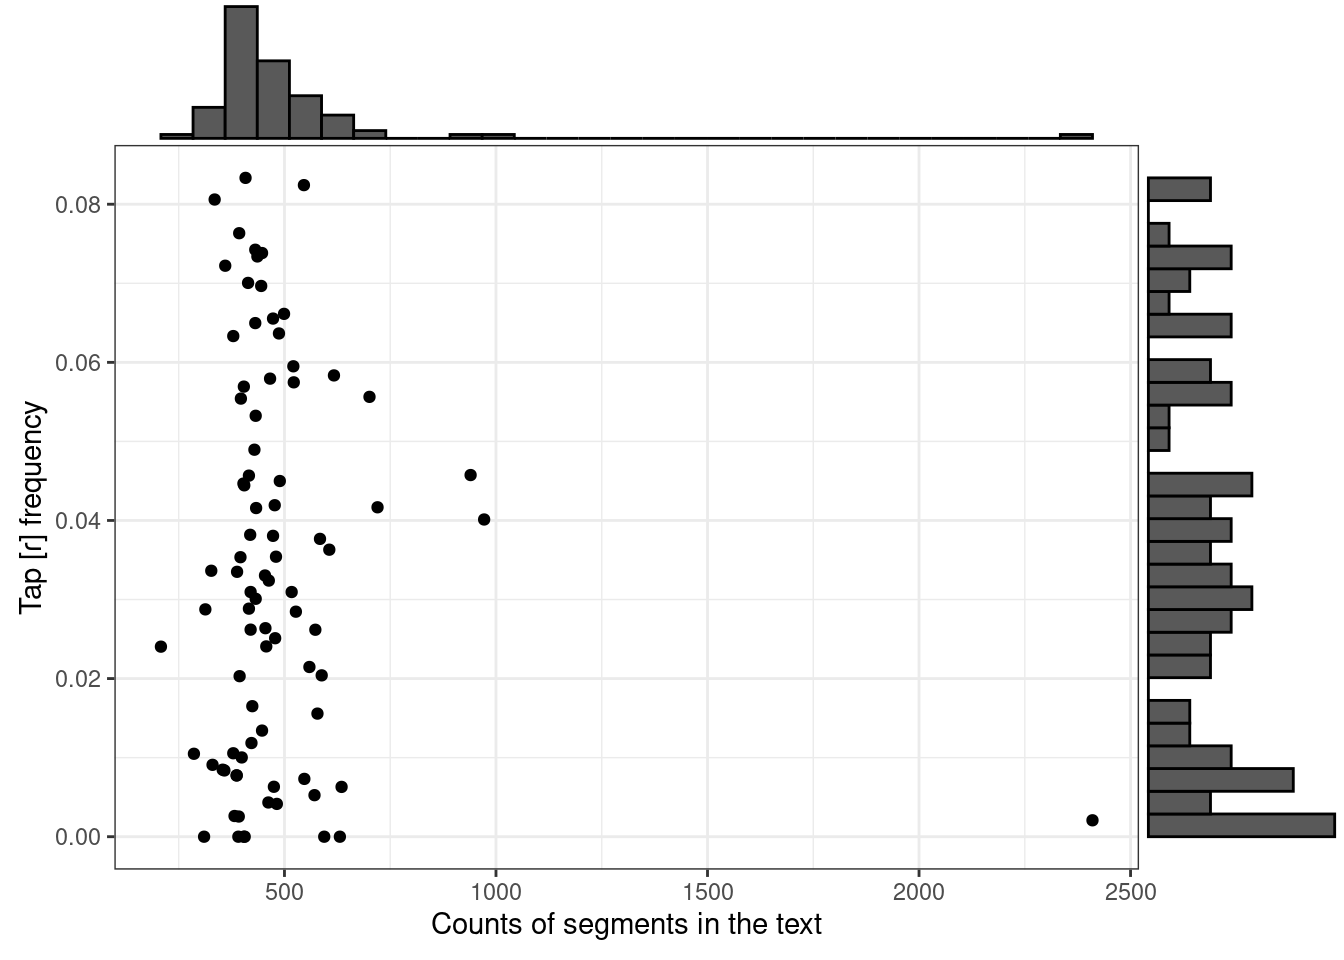
\includegraphics[width=0.75\linewidth]{jipa/images/tap_phonetic_freq}
	\caption[\textrm{[ɾ]} frequency for the 84 transcriptions as a function of the number of segments in the written transcription]{\textrm{[ɾ]} frequency (vertical axis) for the 84 transcriptions as a function of the number of segments in the written transcription (horizontal axis).}
	\label{fig:tapphoneticfreq}
\end{figure}

When looking at the taps in phonetic transcription (\autoref{fig:tapphoneticfreq}), the tap [ɾ] frequency varies between a maximum of 0.083 and a minimum of 0.0 (6 illustrations where there is no [ɾ] in the transcription of the narrative), with a mean of 0.034, a median of 0.032 (both lower than for overall rhoticity), a standard deviation of 0.024, and an interquartile range of 0.045. On the other hand, in phonemic transcription (Figure 13), the tap /ɾ/ frequency varies between a maximum of 0.07 and a minimum of 0.0 (22 illustrations where there is no /ɾ/ in the transcription of the narrative), with a mean of 0.02, and a median of 0.0 (both lower than for overall rhoticity), a standard deviation of 0.024, and an interquartile range of 0.039. The frequency of [ɾ] (0.034) is lower than the rhoticity average (0.048), but is higher than the frequency of /ɾ/. Phonetic taps are more frequent than phonemic taps. A Kruskal–Wallis test shows significant differences for frequency values of phonetic tap, phonemic tap and rhoticity ($H(2)=43.5, p<.0001$), and a post hoc Dunn test shows that all the pairwise differences are statistically significantly different ($p<.01$).

\begin{figure}
	\centering
	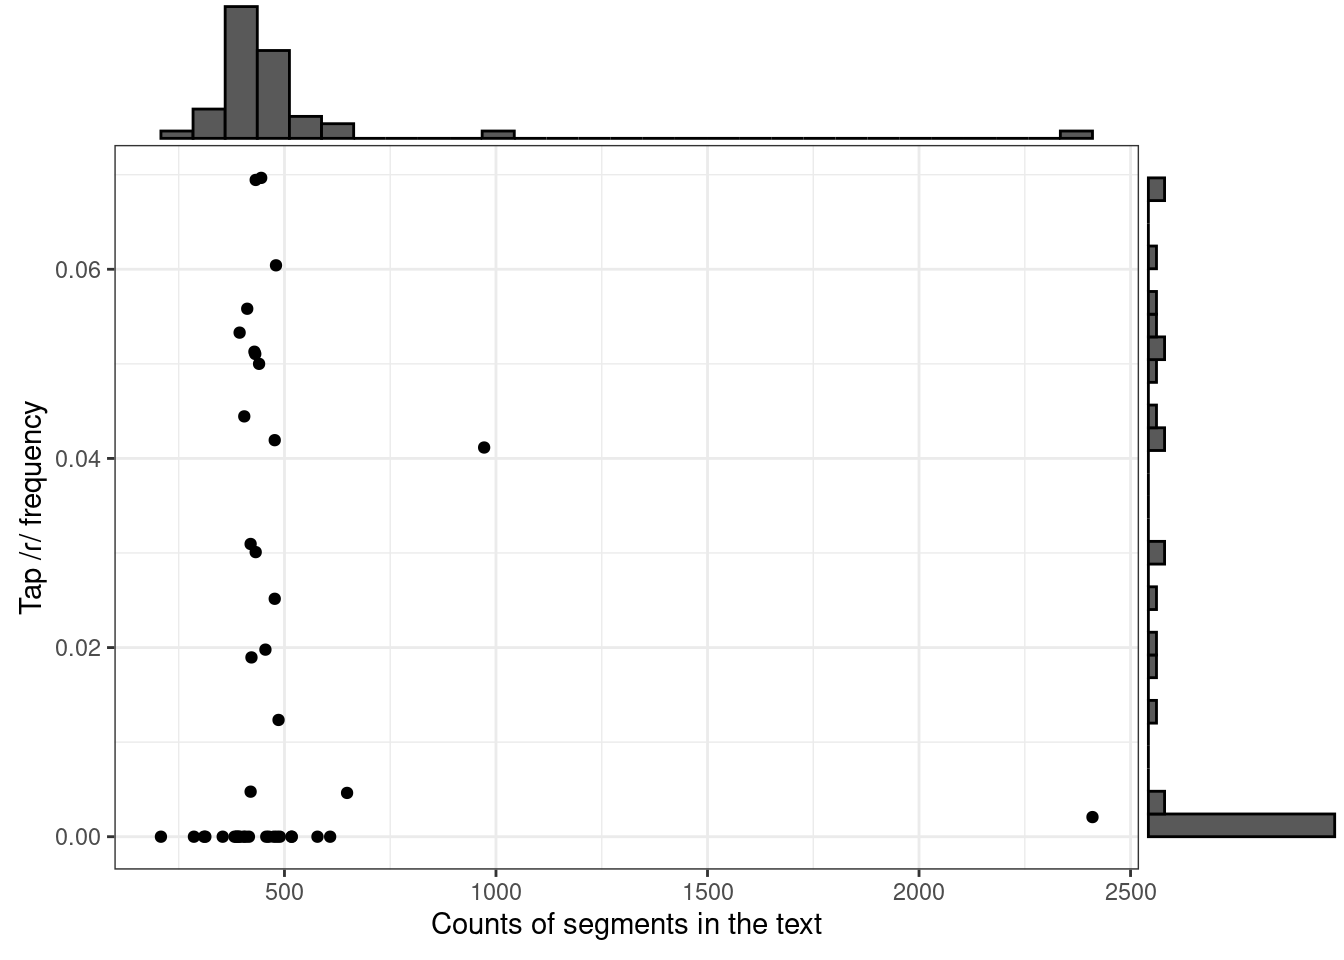
\includegraphics[width=0.75\linewidth]{jipa/images/tap_phonemic_freq}
	\caption[\textrm{/ɾ/} frequency for the 44 transcriptions as a function of the number of segments in the written transcription]{\textrm{/ɾ/} frequency (vertical axis) for the 44 transcriptions as a function of the number of segments in the written transcription (horizontal axis).}
	\label{fig:tapphonemicfreq}
\end{figure}

Finally, we compared the mean frequency of trills, taps and overall rhoticity: the Kruskal–Wallis test shows significant differences for frequency values ($H(4)=82.2, p<.0001$). A post hoc Dunn test showed that phonetic trills [r] frequency was not significantly different from the phonemic taps frequency /ɾ/, that phonemic trills /r/ frequency was not significantly different from the phonetic tap [ɾ] frequency, but that /r/ is more frequent than /ɾ/ ($p<.01$) and [r] is less frequent than [ɾ] ($p<.05$).\\

It can be seen that, compared to trills, taps are under–represented in phonemic transcriptions, but they are over–represented in phonetic transcriptions. The perceived abundance of trills is mainly due to their presence in the phonemic transcriptions, where the \textit{r} symbol encompasses, in fact, a multitude of possible phonetic realizations. One of these possible realizations is a tap, and even if phonetic trills are indeed present, they are less frequent than phonetic taps. These results do not explain why linguists choose certain graphic representations of the phonemes they describe, as the illustrations do not provide information on what makes a phonemic trill different from a phonemic tap. In some of the illustrations containing phonemic trills, we found both phonetic trills and taps, and similarly in some illustrations with phonemic taps, we found both phonetic taps and trills. An unequivocal analysis of a lect sound system based solely on its illustration may be unreachable in some cases due to linguist–specific graphemic conventions.

\section{Discussion and conclusions}

The \textit{Illustrations of the IPA} is an invaluable source of information for many types of studies in linguistics and the language sciences in general, as they tend to offer a standardized description of the sounds of the languages concerned. These articles stand on their own in providing the reader with the keys to understanding the conventions used in the phonetic and phonemic transcriptions. Importantly, they are also instrumental in linguistic studies – such as comparative studies – beyond their primary illustrative goal.\\

While, for some phonemes, transcription conventions are rich and accompanied by detailed descriptions of their different allophones, their context, and even, in some cases, by acoustic measurements, it appears that for rhotics such detailed information is often missing. This contributes to a lack of clarity in the literature concerning their characteristics and cross–linguistic frequency. While this situation seems to be improving in more recent illustrations, this lack of clarity was the reason for our study here. Rhotics are often represented through the symbol \textit{r}, but behind this seemingly simple choice there is a bewildering heterogeneity and complexity of realizations, as has been clearly shown for several languages (Spanish \parencites{blecuaVibrantesEspanolManifestaciones2002,bradleyRhoticVariationConstrast2012,henriksenAcousticAnalysisRhotic2015,vigilRhoticsTaosNew2018}, Dutch \parencite{sebregtsSociophoneticsPhonologyDutch2014}, Portuguese \parencite{rennickeVariationChangeRhotics2015}, English \parencites{stuart-smithDerhoticisationScottishEnglish2014,jauriberryRhotiquesRhoticiteEcosse2016}, Italian \parencite{romano2013preliminary}, Japanese \parencite{magnusonWhatSoundsKansai2008}, Persian \parencite{rafatSocioPhoneticInvestigationRhotics2010}).\\

This chapter quantifies, using a careful analysis of 213 \textit{Illustrations of the IPA} articles, the impression – shared by several linguists – that trills might be over–represented in the literature. We find that, although the phoneme /r/ is not rare (105 illustrations do have an /r/), [r] seems to become less and less frequent as one approaches the phonetic reality (here, as captured to various degrees by the phonetic transcriptions present in some of the illustrations). In other words, even with a transcription material as short as the North Wind and the Sun, we find consistent clues that the r trill symbol tends to be used as the default symbol for rhotics, echoing for instance Sebregts (2014) position:

\begin{displayquote}
~[...] the high cross–linguistic frequency of trill phonemes as reported in UPSID may not in fact be at odds with the low frequency of “actual trills” mentioned by \parencite{ladefogedLateralsTrills1977}, as long as the term “trill phoneme” in the sense of the UPSID is taken to mean a phoneme that is potentially realised as a trill, for which the number of actual trill realisations may be quite low. \parencite[157]{sebregtsSociophoneticsPhonologyDutch2014}
\end{displayquote}

As explained in this chapter, we consider that this ambiguity results from several factors that led the linguistic community to tolerate a blind spot which mirrors the difficulty of handling rhotics in general and trills in particular. We consequently suggest that clarifying the guidelines on rhotics would improve the gold standard against which \textit{Illustrations} is published as already proposed by \parencite[84]{whitleyRhoticRepresentationProblems2003} by ‘[a]dopt[ing] the macron for specifying a trill [ie. r̄], leaving plain \textbf{r} entirely free for its widely understood value of “any rhotic”’. Beyond this aspect, we would like to emphasize that the illustrations are also integrated ‘as they are’ in secondary sources such as phonological databases. There has indeed been a recent explosion in the availability and use of such databases \parencites{phoible,mortensenAlloVeraMultilingualAllophone2020}, and in their relevance to the exploration of large–scale typological and historical questions. Such databases usually compile data from different sources, among which we can find papers published in \textit{JIPA} (as, for example, in PHOIBLE and ALLOVERA). Irrespective of their intended nature (phonemic, allophonic or phonetic), they make use of the symbols proposed by transcription systems, and the symbols of the International Phonetic Alphabet (IPA) are omnipresent and currently almost universally used in linguistics. While they are arguably robust enough for large–scale studies concerning broad phonemic classes and their distribution across language families and geographical areas, our findings highlight that taking them at face value might not be sufficient for research aiming at uncovering subtle effects involving actual acoustic and/or articulatory features (such as those involving sound symbolism, the acoustic adaptation to the environment or weak effects of normal variation in the anatomy of the vocal tract). We hope that, in the near to medium future, this type of large–scale study will be able to better take into account the uncertainty concerning the actual sounds purportedly described by a symbol (and, of particular importance here, the trill), either through the availability of finer–grained data or of ways to probabilistically map a given symbol to a set of possible realizations in a given context. \\ 

Thus, our work should help better understand the current theories concerning the visual representation of languages, to judge their advantages, disadvantages and limits \parencites{whitleyRhoticRepresentationProblems2003,eslingPhoneticNotation2010,andersonCrosslinguisticDatabasePhonetic2018}.  \\    

To conclude, while we do not think there is a single ‘silver bullet’ that can solve all these issues, we suggest extra caution in the way phonetic symbols are interpreted, especially for older sources, and to contextualize them relative to the various transcription systems in use at the time and even relative to the reforms of the International Phonetic Association.

\begingroup
\sloppy

\chapter{Description acoustique du \textit{r} dans les \textit{Illustrations of the IPA}} \label{chap:acoustics}
\epigraph{\href{https://www.bilibili.com/video/BV19f4y1W7Qu/}{{\cjkfont 齿龈颤音}}}

\renewcommand{\chapterautorefname}{chapitre}
\renewcommand{\sectionautorefname}{section}
\renewcommand{\subsectionautorefname}{sous-section}
\renewcommand{\subsubsectionautorefname}{sous-sous-section}

La section acoustique de cette thèse cherche à donner de nouveaux éléments de réponse à la question relative à la fréquence cross-linguistique des trills. Cette section s'intéresse directement au signal acoustique à travers la création de catégories auxquelles des motifs de sons \textg{simil-r} peuvent appartenir. Nous nous concentrons sur deux niveaux d'analyse pour comprendre ce que le trill subsume. D'un côté, nous créons des catégories pour mettre en évidence les principaux motifs acoustiques visibles, et de l'autre côté, nous utilisons un niveau d'analyse plus fin pour appréhender la substance des trills, et en mesurer la durée. Nous opposons donc un niveau phonologique à un niveau proche de la réalité phonétique.\\

Les travaux présentés sont complémentaires à ceux du \autoref{chap:jipa} qui cherchait à répondre à la même question en regardant directement les transcriptions disponibles dans les différentes \textit{Illustrations of the IPA}, dans la mesure où il s'agit de la même source d'information. Nous avons pris les audios de la Bise et le Soleil associés aux articles. À chaque article est généralement associé l'audio d'un locuteur ou d'une locutrice récitant la fable dans leur variété de langue (la transcription étroite de l'enregistrement du français est reproduite ci-dessous). Certains auteurs/trices des \textit{Illustrations of the IPA} peuvent choisir d'inclure une histoire différente car iels considèrent que la fable d'Ésope n'est pas appropriée pour travailler avec les locuteurs. Généralement, les arguments sont, d'une part, que l'intrigue est trop abstraite et demande beaucoup d'imagination de la part de l'informateur/trice et, d'autre part, que malgré le type de prononciation familière visée, la fable peut donner lieu à un style plutôt formel. Pour ces deux raisons, le texte a dû être paraphrasé lors de sa lecture aux informateurs/trices \parencite{capellTranscriptionVowelConsonant1979,ternesNorthWindSun1975} et dans certaines situations, l'illustration s'est retrouvée avec une histoire ou un texte différent \parencite{guerinMavea2009,edwardsAmarasi2016}. Nous ne ferons pas de distinction entre les différents types de récits dans ce chapitre.

\begin{displayquote}
	{\fontspec{Charis SIL}\small la biz e lə sɔlɛʲ sə dispytɛ ‖ ʃakɛ̃ asyʁɑ̃ kilɛtɛ lə ply fɔ̈ʁ̞ ‖ kɑ̃t ilzɔ̃ vy ɛ̃
	vwɑjaʒœ ki savɑ̃sɛ ‖ ɑ̃vlope dɑ̃ sɔ̃ mɑ̃to ‖ iː sɔ̃ tɔ̃be dakɔ̈ʁ̥ kə səlɥi ki
	aʁivʁe ləpʁ̥əmje a lə lɥi fɛʁote ‖ səʁə ʁəgaʁde kɔ̈m lə ply fɔ̈ʁ̥ ‖ alɔ̈ʁ̞ la
	biz sɛ̝ miz a sufle də tut se fɔ̈ʁ̞s ‖ mɛ ply ɛl suflɛ ply lə vwɑjaʒœʁ̞ sɛʁɛ
	sɔ̃ mɑ̃totʊʁ̞ də lɥi ‖ finalmɑ̃ ɛl ʁənõsa lə lɥi fɛʁote ‖ alɔ̈ʁ̞ lə sɔlɛʲ kɔmɑ̃sa
	bʁ̥ije ‖ e o bu dɛ̹̃ mɔmɑ̃ lə vwɑjaʒœ ʁeʃofe ota sɔ̃ mɑ̃to ‖ ɛ̃si la biz dy
	ʁəkɔnɛt kə lə sɔlɛʲ ɛtɛ lə ply fɔ̈ʁ̞.}\\
	\parencite[75]{fougeronFrench1993}
\end{displayquote}


Les enregistrements sonores des \textit{Illustrations of the IPA} représentent donc une source précieuse d'informations pour une étude comparative acoustique par la longueur des enregistrements (autour d'une minute généralement), et la diversité des variétés enregistrées. Néanmoins, le faible nombre de personnes enregistrées par article rend ardue la distinction entre ce qui relève de l'idiolecte et ce qui relève de la langue.\\

Nous proposons deux études où nous avons segmenté et annoté des rhotiques en suivant deux méthodologies.
La première étude repose sur 73 langues issues de 16 familles linguistiques (\autoref{tab:fam73}). Nous avons cherché des motifs à partir des oscillogrammes et des spectrogrammes dans le but d'obtenir quatre grandes classes, c'est-à-dire des catégories, de rhotiques. La méthodologie utilisée dans cette première étude permet de mettre en évidence que la catégorie qui correspond à un trill avec au moins deux occlusions distinctes n'est pas si fréquente dans les langues étudiées. De plus, elle permet de mettre en avant les problèmes de la segmentation et de l'annotation des rhotiques.

\begin{table}

\begin{tabular}{llc}
	\hline
	Famille de langues & Glottocode & Nombre de langues incluses \\
	\hline
	Langues chamito-sémitiques & afro1255 & 10 \\

	Langues atlantico-congolaises & atla1278 & 4 \\

	Langues austronésiennes & aust1307 & 13 \\

	Langue basque & basq1248 & 1 \\

	Langues yumanes & coch1271	 & 1 \\

	Langues dravidiennes & drav1251 & 1 \\

	Langues indo-européennes & indo1319 & 28 \\

	Langue kuanama & kuna1268 & 1 \\
	
	Langues morehead-maro & more1255 & 1 \\

	Langues oto-mangues & otom1299	 & 2 \\

	Langues pama-nyungan  & pama1250 & 4 \\

	Langues sino-tibétaines & sino1245 & 2 \\

	Langues taï-kadaï & taik1256 & 1 \\

	Langues timor-alor-pantar & timo1261 & 1 \\

	Langues turciques & turk1311 & 1 \\

	Langues ouraliennes & ural1272 & 2 \\
	\hline
\end{tabular}
\caption[Familles de langues incluses dans la première étude acoustique]{Familles de langues incluses dans la première étude acoustique, ainsi que le nombre de langues incluses par famille.} \label{tab:fam73}
\end{table}

La deuxième méthodologie repose sur moins de données. Nous avons resegmenté et réannoté 18 langues de notre échantillon initial de 73 langues issues de 7 familles linguistiques. Cette méthodologie repose en grande partie sur les travaux de \citeauthor{blecuaVibrantesEspanolManifestaciones2002}. Il s'agit d'étudier les trills et les taps à travers leurs différents composants. Bien que les langues soient issues de l'échantillon initial, nous n'opérons pas de comparaison systématique entre les deux méthodologies.\\

Dans ce chapitre, indépendamment de la méthodologie utilisée, nous cherchons à explorer la variation dans les rhotiques à partir des \href{https://richardbeare.github.io/marijatabain/ipa_illustrations_all.html}{enregistrements sonores}\footnote{Les enregistrements sonores sont disponibles à l'adresse suivante : \url{https://richardbeare.github.io/marijatabain/ipa\_illustrations\_all.html}} inclus dans les \textit{Illustrations of the IPA} et à mettre en évidence que les /r/ à un contact ou sans contact sont plus fréquents que les /r/ à plus d'un contact. Pour cela, dans un premier temps, nous allons voir comment les rhotiques, et en particulier les trills et les taps, ont été étudiés avec un intérêt particulier pour deux différentes méthodologies utilisées dans des études sur des langues diverses. Dans les deux cas, il s'agit d'analyses préliminaires avec des données déjà existantes et donc non collectées dans le but d'étudier les rhotiques.

\section{Les études acoustiques sur la variation dans le trill et le tap}

\subsection{La composition des trills et des taps : la thèse de \citeauthor{blecuaVibrantesEspanolManifestaciones2002} sur l'espagnol}

Dans un premier temps, nous nous intéressons à la thèse de \textcite{blecuaVibrantesEspanolManifestaciones2002} qui observe la composition des trills et des taps, deux phonèmes de l'espagnol. À travers des analyses acoustiques sur un corpus de parole lue (à laquelle l'autrice fait référence comme parole de laboratoire en opposition à la parole spontanée), elle souhaite mettre en avant les facteurs influençant les réalisations. Pour cela, elle inclut, dans son étude, deux locuteurs hommes âgés de 28 ans et 34 ans ayant été à l’université.\\

Ses analyses se concentrent sur les phonèmes tap et trill dans trois positions : en position intervocalique, en seconde position d'un groupe consonantique en attaque de mot, et dans le mot avant une consonne hétérosyllabique. De fait, la position initiale n'est pas prise en compte ainsi que celle en position finale de mot. Un des buts de la thèse de \citeauthor{blecuaVibrantesEspanolManifestaciones2002} est de déterminer quelle est la forme canonique (l'allophone canonique, le plus représentatif) dans chaque position.\\

L'élaboration du corpus s'est faite en contrôlant les différents contextes possibles avec les consonnes et les voyelles, ainsi que l'accent. Les locuteurs enregistrés ont pu lire une première fois la feuille avec ce qu'ils devaient répéter, et ont pu se corriger lorsqu'ils commettaient des erreurs de lecture. Il n'est pas explicité de quel type d'erreur il s'agit. La fréquence d'échantillonnage, le nombre de mesure du signal par seconde, utilisée pour les enregistrements, est de 10000 Hz.\footnote{Le signal acoustique est converti en signal électrique puis numérisé. Pour cela plusieurs standards de fréquences d'échantillonnage existent. Le standard actuel dans les études de la parole humaine est de 44100 Hz (le double, suite au théorème de Nyquist-Shannon, de 22050 Hz qui est considéré comme le seuil maximum de perception des nouveaux nés).}\\

Son analyse acoustique se base sur la recherche « de composants ». Ces éléments qui composent la rhotique peuvent correspondre à des éléments vocaliques épenthétiques « svarabhaktiques » vocaliques (\textg{elemento esvarabático}), des phases de silence avec barre de voisement correspondant à une occlusion (même si \citeauthor{blecuaVibrantesEspanolManifestaciones2002} (p. 30) rappelait que \textg{las fases cerradas no necesariamente se manifiestan como silencios, sino que lo imprescindible es que la energía sea menos intensa que en las fases abiertas}\footnote{\textg{[Trad.] les phases fermées ne se manifestent pas nécessairement comme des silences, mais il est essentiel que l'énergie soit moins intense que dans les phases ouvertes.}}), des composants avec une structure formantique similaire à une approximante et des composants avec friction. Lorsqu’il y a plus de trois composants, \citeauthor{blecuaVibrantesEspanolManifestaciones2002} parle de groupes multiples.\\

Il est intéressant de noter que certaines réalisations du /r/ et du /ɾ/ peuvent être identiques par leurs composants qui sont soit un composant \textg{approximante} soit un composant \textg{occlusion}.\\

Les paramètres acoustiques utilisés pour la classification sont de deux types. D'un côté, la durée totale de la vibrante a été prise en compte, de même que la durée des différents composants et des voyelles adjacentes. \citeauthor{blecuaVibrantesEspanolManifestaciones2002} ne donne pas de critères de segmentation. On retrouve cependant des exemples, illustrés avec des spectrogrammes, des différents éléments qu'elle considère. \citeauthor{blecuaVibrantesEspanolManifestaciones2002} est consciente de l'importance de bien segmenter (pp. 31-32).
Les fréquences des formants (F1, F2 et F3) ont aussi été prises en compte. La mesure des formants a été faite sur les éléments vocaliques (comme sur les éléments « escarabatico » ou les éléments vocaliques présents dans les groupe multiples) mais aussi sur les approximantes. De plus, des mesures ont été faites sur les voyelles ou approximantes adjacentes.
\citeauthor{blecuaVibrantesEspanolManifestaciones2002} ne s'intéresse pas directement au contour de l'intensité pour faire sa catégorisation des rhotiques.\\

La thèse de \citeauthor{blecuaVibrantesEspanolManifestaciones2002} repose sur des éléments, les composants des trills et des taps. Il ne s'agit pas de catégoriser immédiatement les segments avec différents symboles de l'API mais de pousser dans le détail la composition des sons. Nous souhaitons confronter cette méthodologie à une multitude de langues pour vérifier si elle est robuste et permet de mettre en évidence différents motifs, différentes combinaisons d'éléments dans différentes langues.

\subsection{Travaux sur la base de catégories API : le néerlandais et le japonais}

La thèse de \textcite{sebregtsSociophoneticsPhonologyDutch2014} se distingue de celle de \citeauthor{blecuaVibrantesEspanolManifestaciones2002} en ce qu'il n'y a pas eu de segmentation, seulement de l'annotation (\textg{coding}) des différents variants sur la base d'un classement établi à partir de la littérature variationniste du néerlandais et des données récoltées. Dans le cadre d'un vaste projet\footnote{Les porteurs du projet \textit{r-kennen, socio-dialectological, phonetic and phonological qualities of /r/ in Dutch} étaient Hans Van de Velde and Wim Zonneveld.}, il a travaillé sur 408 locuteurs pour quelques 21006 occurrences de r sur dix accents urbains des Pays-bas, là où \citeauthor{blecuaVibrantesEspanolManifestaciones2002} n'avait que deux locuteurs. Ces 21006 occurrences, dans des contextes variés mais contrôlés, ont été annotées par Evie Tops et l'auteur lui-même.\\

Les variants inclus étaient :

\begin{itemize}
	\item Le trill voisé alvéolaire [r]
	\item Le trill alvéolaire partiellement dévoisé [r͡r̥]
	\item Le trill alvéolaire non voisé [r̥]
	\item Le trill ou tap avec de la friction homorganique [r͡ɹ̝]
	\item La fricative (post)alvéolaire voisée [ɹ̝]
	\item La fricative (post)alvéolaire non voisée [ɹ̥]\footnote{[\textit{sic}] pour la transcription utilisée}
	\item Le tap alvéolaire voisé [ɾ]
	\item Le tap alvéolaire non voisé [ɾ̥] 
	\item L'approximante alvéolaire [ɹ]
	\item Le trill uvulaire [ʀ]
	\item Le trill fricatif uvulaire [ʀ̝]
	\item La fricative uvulaire [ʁ]
	\item L'approximante uvulaire [ʁ̞]
	\item L'approximante rétroflexe ou \textg{bunched} [ɻ]
	\item L'approximante palatale [j]
	\item La voyelle antérieure basse-moyenne [ɛ]
	\item La voyelle centrale [ə]
	\item La voyelle basse [ɐ]
	\item L'élision du r avec rétraction de la consonne suivante : ØC̠
	\item L'élision du r : Ø
\end{itemize}

\citeauthor{sebregtsSociophoneticsPhonologyDutch2014} inclut aussi une description acoustique de chacun des variants avec dans certains cas des détails sur la structure formantique. Pour le trill alvéolaire, on retrouve donc quatre sous-variants [r], [r͡r̥], [r̥] et [r͡ɹ̝]. \\

Pour le japonais kansai, \textcite{magnusonWhatSoundsKansai2008} analyse le discours de quatre locuteurs. L'auteur définit des domaines du \textit{r} (\textg{r-domain}) (pp. 45-46) entre des pics d'amplitude de voyelles, pour la segmentation. Sa transcription se base sur les symboles de l'API prenant en compte les symboles [d ɾ l ɺ ɹ]\footnote{\textcite{magnusonWhatSoundsKansai2008} utilise uniquement le terme de \textg{flap} (et non pas celui de \textg{tap}).} ainsi que des diacritiques comme, par exemple, la palatalisation ou le dévoisement. Par exemple ɾ̝ est un flap élevé se traduisant par \textg{a greater interruption of surrounding vowels’ resonance in a manner akin to, but less than, release bursts associated with voiced stops} (p. 52) qui se révèle être le plus fréquent dans son corpus (14,2\%) (p. 58). Ce segment est illustré en \autoref{fig:figure7magnuson}.\\

\begin{figure}
	\centering
	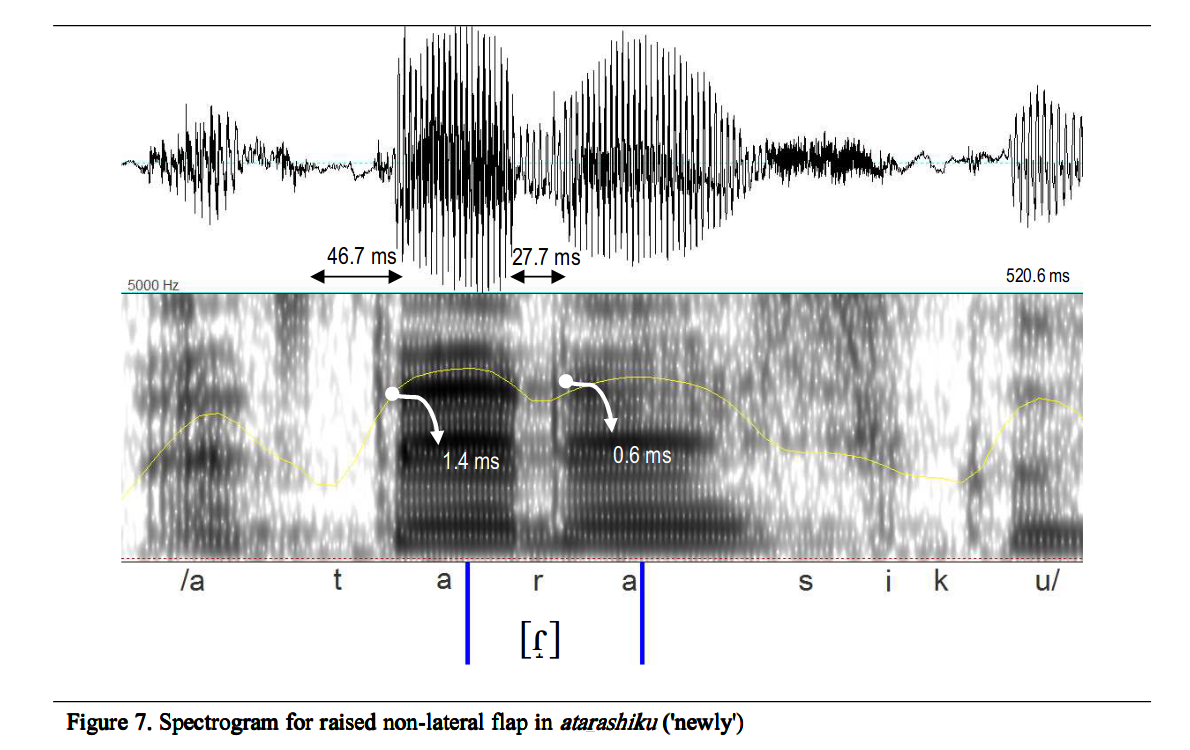
\includegraphics[width=0.8\linewidth]{substance/images/figure7_magnuson}
	\caption[Illustration du  ɾ̝  par \textcite{magnusonWhatSoundsKansai2008}]{Illustration du  ɾ̝  par \textcite[p.61]{magnusonWhatSoundsKansai2008} avec un oscillogramme en haut, et un spectrogramme en bas. La durée du /t/ est de 46,7 ms dont 1,4 ms pour la phase de relâchement contre une durée de 27,7 ms pour le /r/ dont 0,6 ms pour la phase de relâchement.}
	\label{fig:figure7magnuson}
\end{figure}

Nous avons choisi de ne pas adopter cette méthodologie pour les langues sur lesquelles nous travaillons. En effet, cette méthodologie est chronophage et implique une vision globale des données, comme \citeauthor{sebregtsSociophoneticsPhonologyDutch2014} l'indique dès le début de sa thèse dans ses remerciements : \textg{[...] that process was a laborious one of defining and redefining categories, listening and relistening and re-relistening to thousands of tokens.} (p. xi). Elle demande aussi, quand c'est possible, d'avoir plusieurs transcripteurs, ou de revenir a posteriori sur les annotations (ici un mois plus tard) comme \textcite{magnusonWhatSoundsKansai2008} l'a fait car il était seul face à ses données, et ce, afin de mesurer sa cohérence. Notre but principal n'étant pas de mesurer la variation de la rhotique, nous avons fait le choix de ne suivre ni la méthode d'annotation a posteriori de \textcite{magnusonWhatSoundsKansai2008} ni de demander à une deuxième personne de transcrire et d'annoter avec nous.


\subsection{Travaux sur la base de catégories plus larges : le malayalam et le persan}

Le malayalam contraste au moins deux rhotiques qui peuvent être décrites soit comme étant une opposition entre un trill et un tap, soit comme deux trills avec le lieu d'articulation les contrastant. L'\textit{Illustration of the IPA} \cite{namboodiripadMalayalamNamboodiriDialect2017a} sur le dialecte namboodiri du malayalam fait état d'une opposition entre un segment trill /r/ et un segment tap or flap /ɾ/. On retrouve également dans l'inventaire une approximante rétroflexe /ɻ/.\\

\citeauthor{punnooseAuditoryAcousticStudy2010} a identifié seulement cinq variants différents dans sa thèse. Il s'agit des segments suivants :

\begin{itemize}
	\item Le tap approximant
	\item Le trill approximant
	\item Le tap canonique
	\item La séquence trill + voyelle épenthétique
	\item Le trill multi-contacts
\end{itemize}

Lors de ses recherches en socio-phonétique sur le persan, \textcite{rafatSocioPhoneticInvestigationRhotics2010} code quatre catégories. Son étude inclut deux locuteurs et trois locutrices tous/toutes titulaires (ou en cours d'obtention) d'un diplôme de l'éducation supérieure. Les catégories sont utiles pour classer les rhotiques des mots issus d'une tâche de lecture de mot, et une tâche de mémorisation de mots, censée être plus spontanée. Dans son étude, le trill est caractérisé par des phases d'ouvertures et de fermetures présentes sur un spectrogramme à bandes larges; le tap n'est pas décrit; la fricative est caractérisée par l'absence de structure formantique et la présence de bruit; et l'approximante est caractérisée par une structure formantique et un signal périodique.\\


Il est important de faire le lien entre deux types de méthodologie. D'un côté, on retrouve la méthodologie de \textcite{blecuaVibrantesEspanolManifestaciones2002} qui s'intéresse à la composition des trills et des taps. De l'autre côté, l'important est l'élaboration de catégories sur la base de motifs acoustiques. En effet, on retrouve les symboles API avec \textcite{sebregtsSociophoneticsPhonologyDutch2014} pour le néerlandais, \textcite{patinWashiliShingazidja2013} pour le washili shingazidjan (non développé ici) ou encore \textcite{magnusonWhatSoundsKansai2008} pour le japonais. Et on retrouve des catégories sans aucun symbole avec \textcite{rafatSocioPhoneticInvestigationRhotics2010} pour le perse ou \citeauthor{punnooseAuditoryAcousticStudy2010} pour le malayalam.\\

Nous pensons que l'intégration des différentes méthodologies permet une meilleure compréhension de la distribution typologique du trill et du tap : d'un côté nous aurions des catégories qui seraient similaires à celles qu'on pourrait avoir en phonétique segmentale, et d'un autre la substance pouvant être incluse dans ces catégories. Cette substance pourrait être comparée à des gestes articulatoires.


\section{Première étude : classification des trills et taps dans des macro-classes}

\subsection{Quatre catégories différentes}

Nous avons parcouru tous les enregistrements sonores des narratives des \textit{illustrations of the IPA}. Nous avons eu accès à 81 enregistrements pour 75 langues. Pour certaines illustrations plusieurs personnes pouvaient être enregistrées.\\

Nous avons fait le choix, dès le début, d'opter pour une annotation sans symbole API. Ces catégories sont similaires à celles adoptées par \textcite{rafatSocioPhoneticInvestigationRhotics2010} car suffisamment larges pour permettre la catégorisation d'un maximum de réalisations des rhotiques, tout en ciblant les productions à plusieurs occlusions.
Ainsi, nous avons commencé notre annotation par quatre catégories : \textg{t1}, \textg{t2}, \textg{t3} et \textg{t4}.\\

La catégorie \textg{t1} fait référence à un segment à une occlusion courte (\autoref{fig:haus125777110}). Au niveau du spectrogramme, on retrouve une zone d'énergie moins importante qui s'observe au niveau du signal par une baisse de l'amplitude et de l'intensité du signal.\\

\begin{figure}
	\centering
	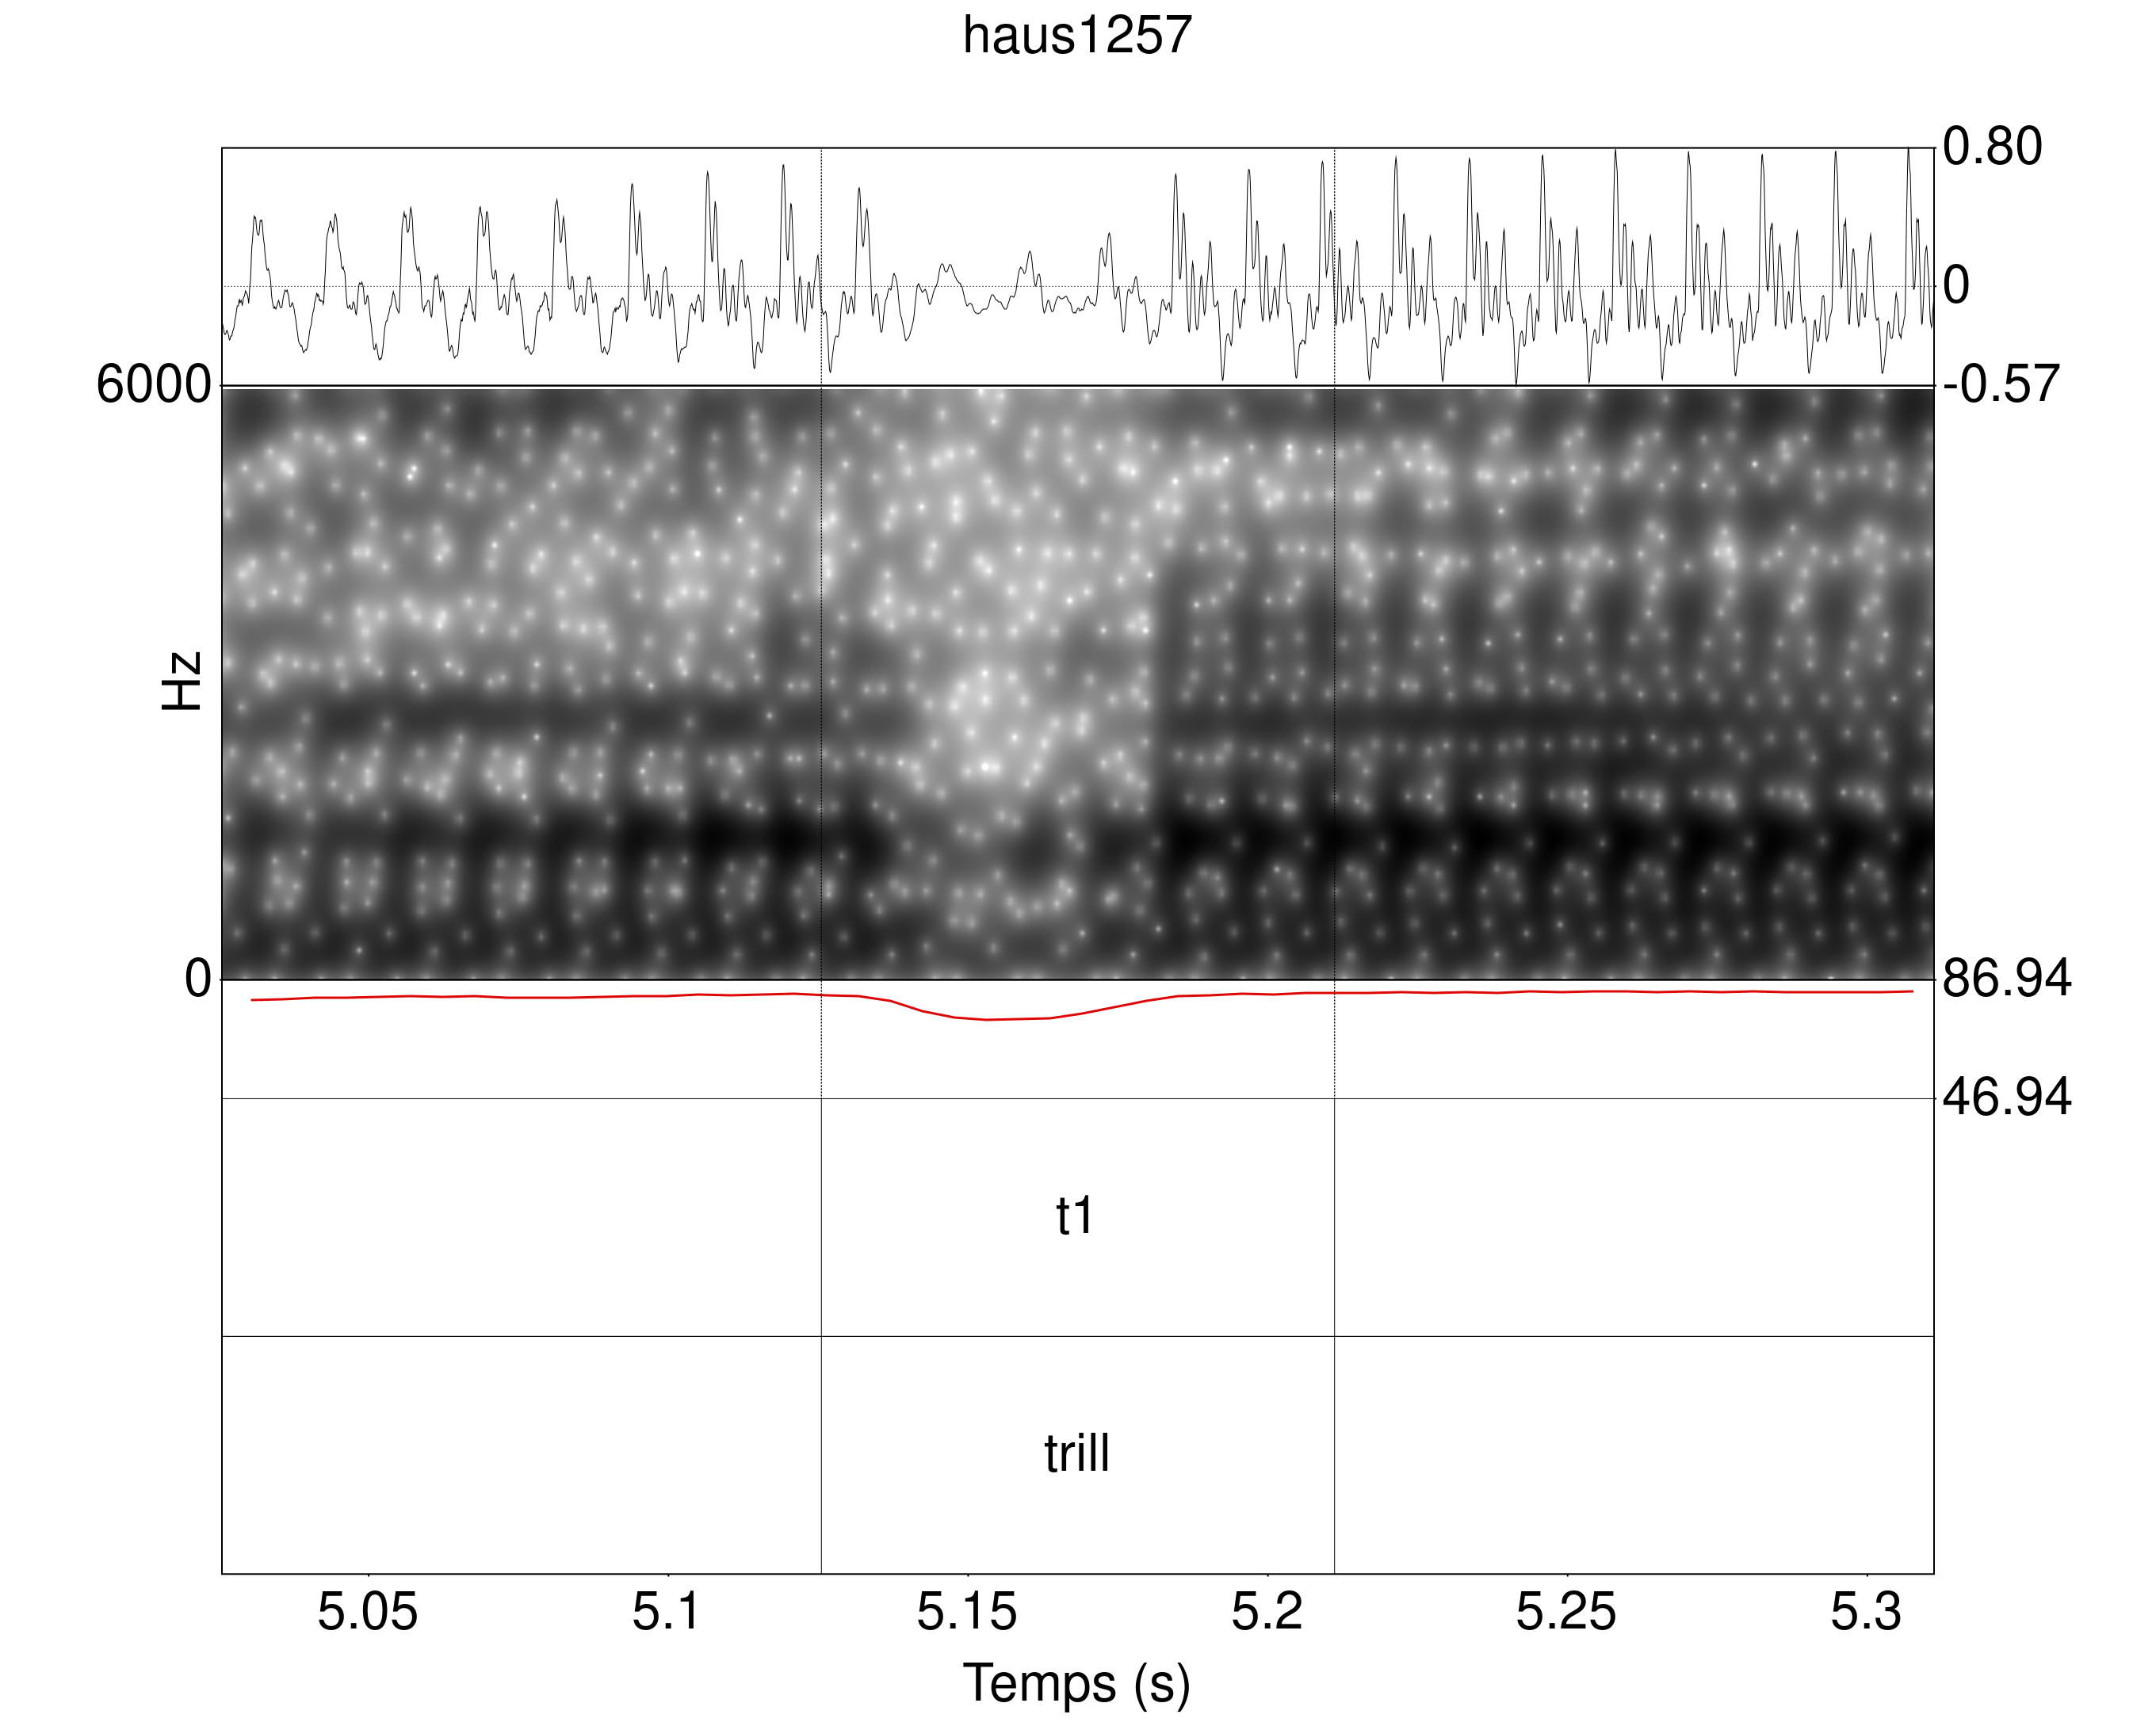
\includegraphics[width=0.8\linewidth]{substance/spectro_images/haus1257_768_4}
	\caption[Illustration de la catégorie \textg{t1}]{Illustration de la catégorie \textg{t1} dans le contexte [wɘtɘ raːnaː] en hausa \glotto{haus1257}. De haut en bas, nous avons l'oscillogramme, le spectrogramme, la courbe d'intensité, un palier intervallique avec la catégorie segmentée, et un palier intervallique comprenant le label descriptif du segment d'intérêt.}
	\label{fig:haus125777110}
\end{figure}


La catégorie \textg{t2} fait référence à un segment à au moins deux occlusions (\autoref{fig:nenn1238131256}), au moins deux diminutions de l'intensité et donc de l'amplitude du signal.\\

\begin{figure}
	\centering
	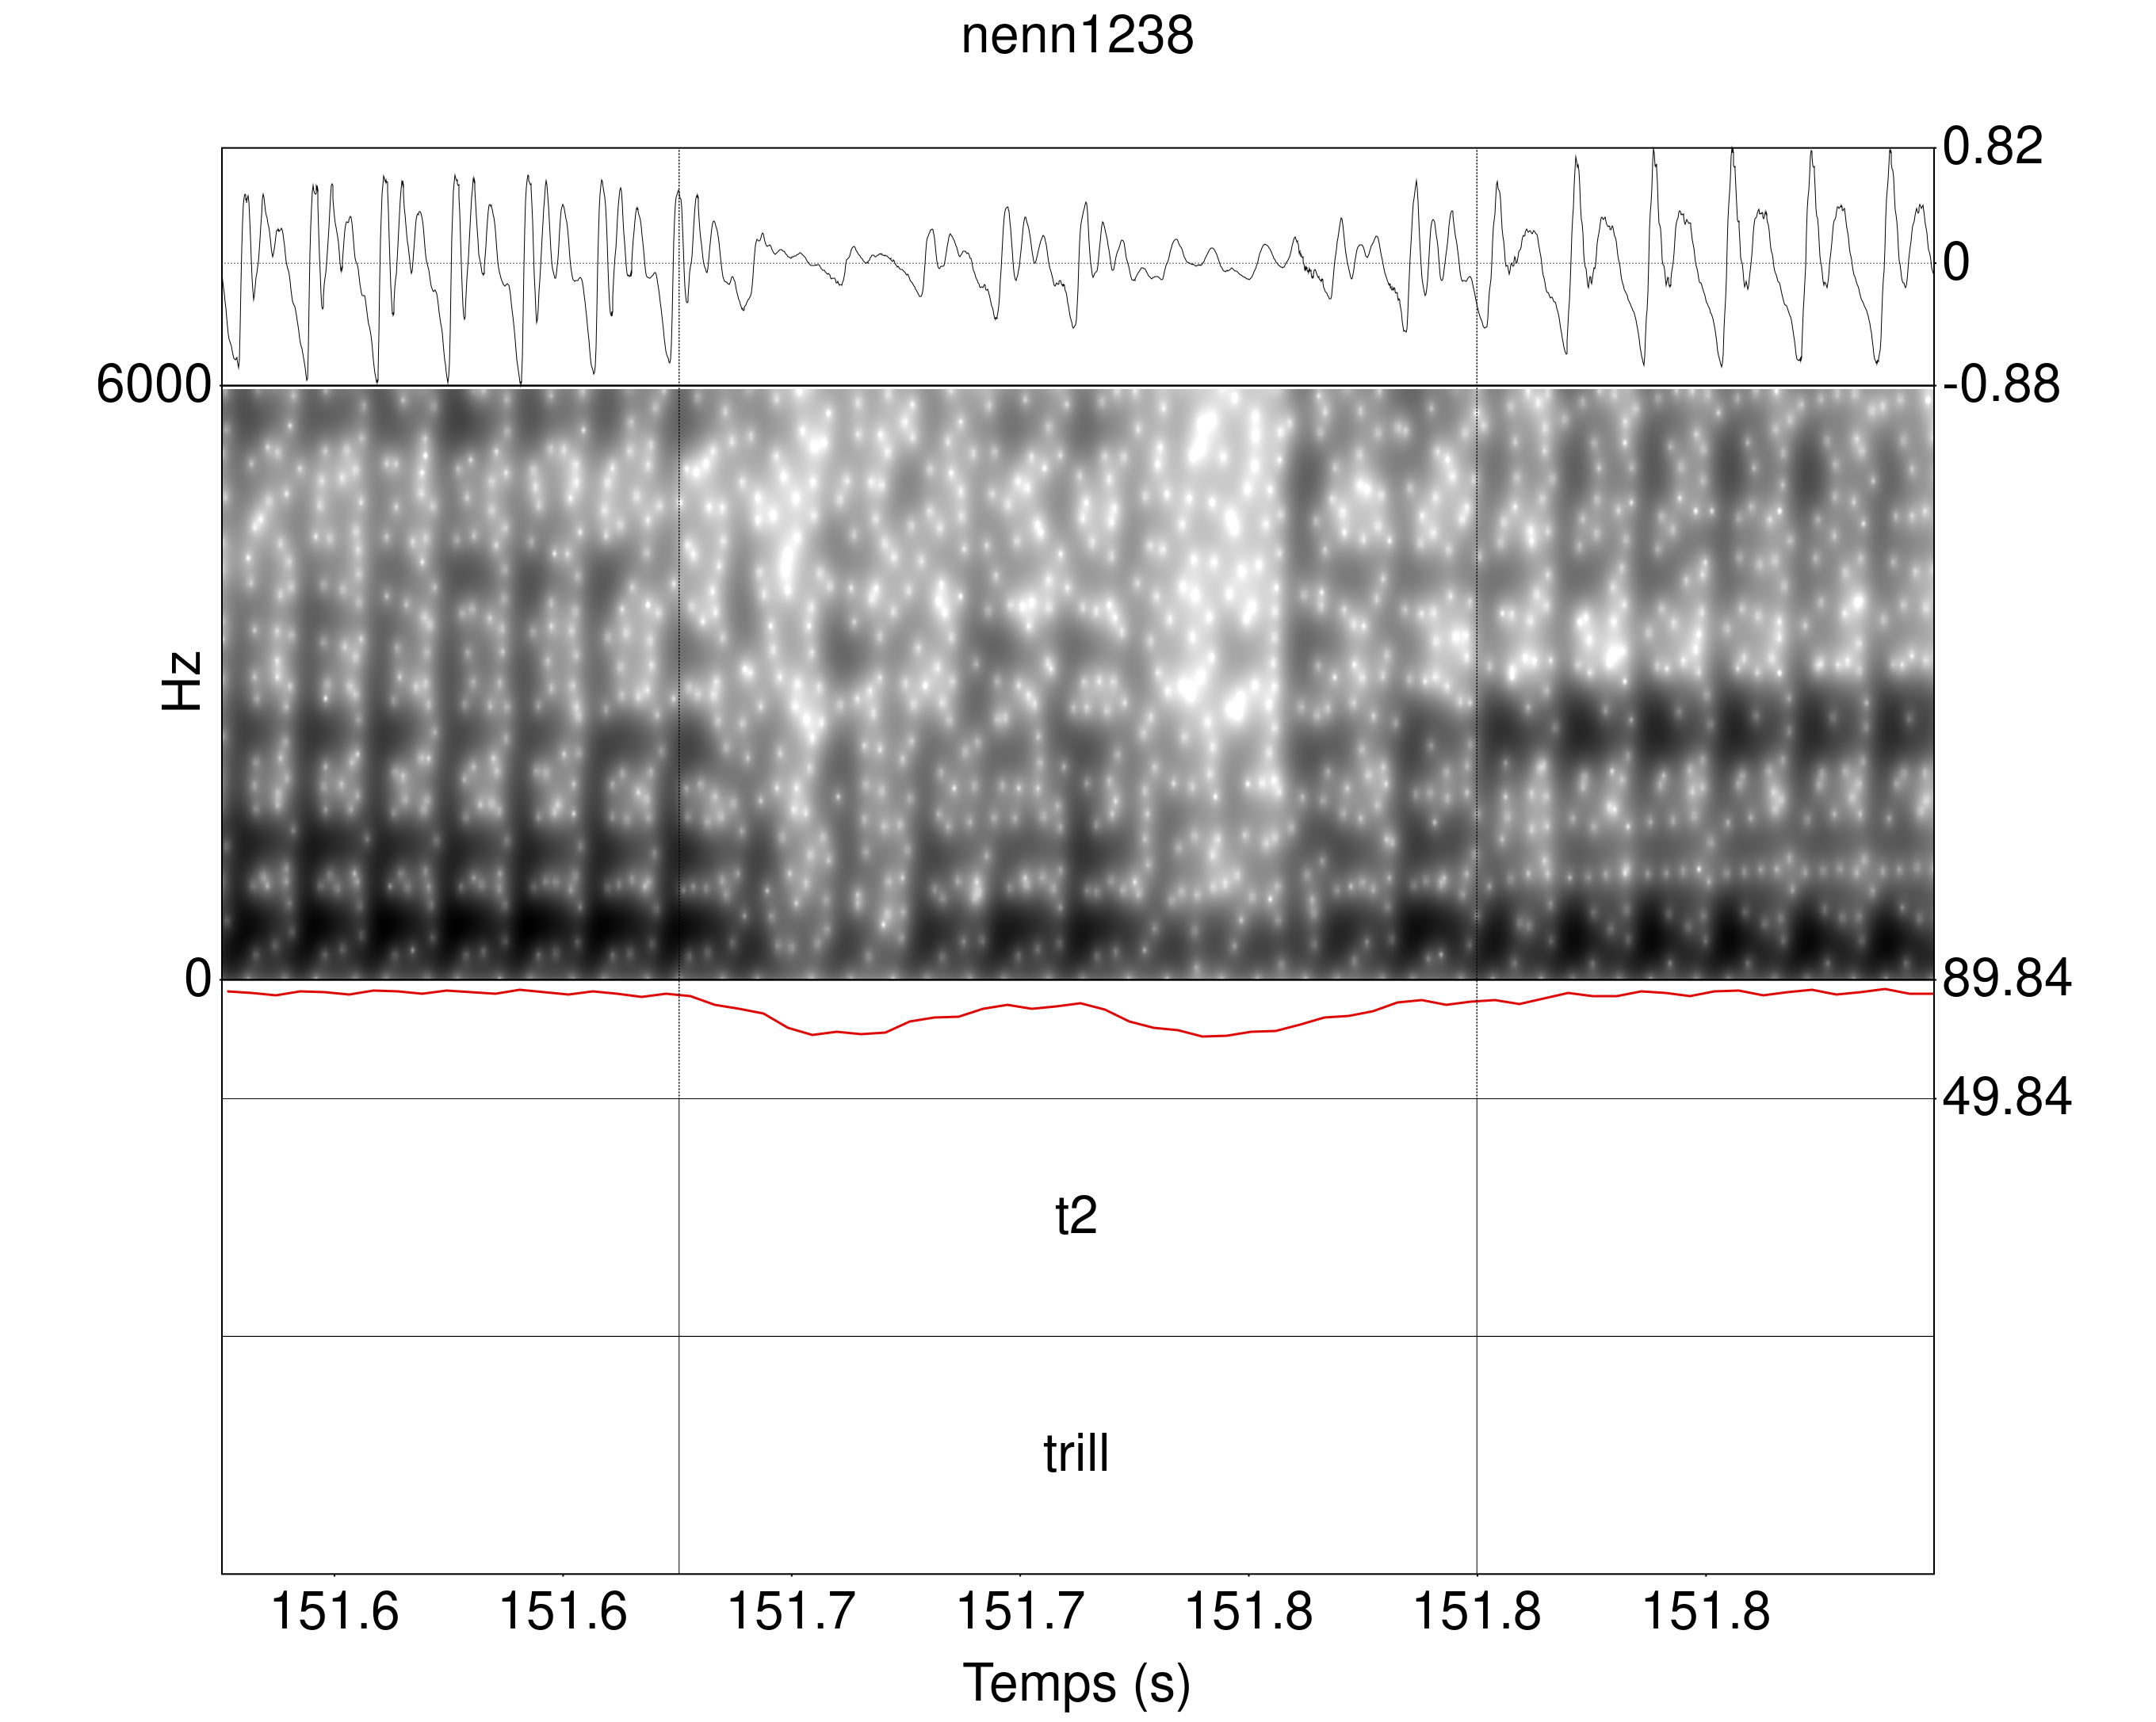
\includegraphics[width=0.8\linewidth]{substance/spectro_images/nenn1238_1312_56}
	\caption[Illustration de la catégorie \textg{t2}]{Illustration de la catégorie \textg{t2} dans le contexte [ˈkesær ˈombtebas] en nen \glotto{nenn1238}. De haut en bas, nous avons l'oscillogramme, le spectrogramme, la courbe d'intensité, un palier intervallique avec la catégorie segmentée, et un palier intervallique comprenant le label descriptif du segment d'intérêt.}
	\label{fig:nenn1238131256}
\end{figure}

La catégorie \textg{t3} fait référence à un segment contenant du bruit similaire à celui qu'on retrouve dans les fricatives.\\

\begin{figure}
	\centering
	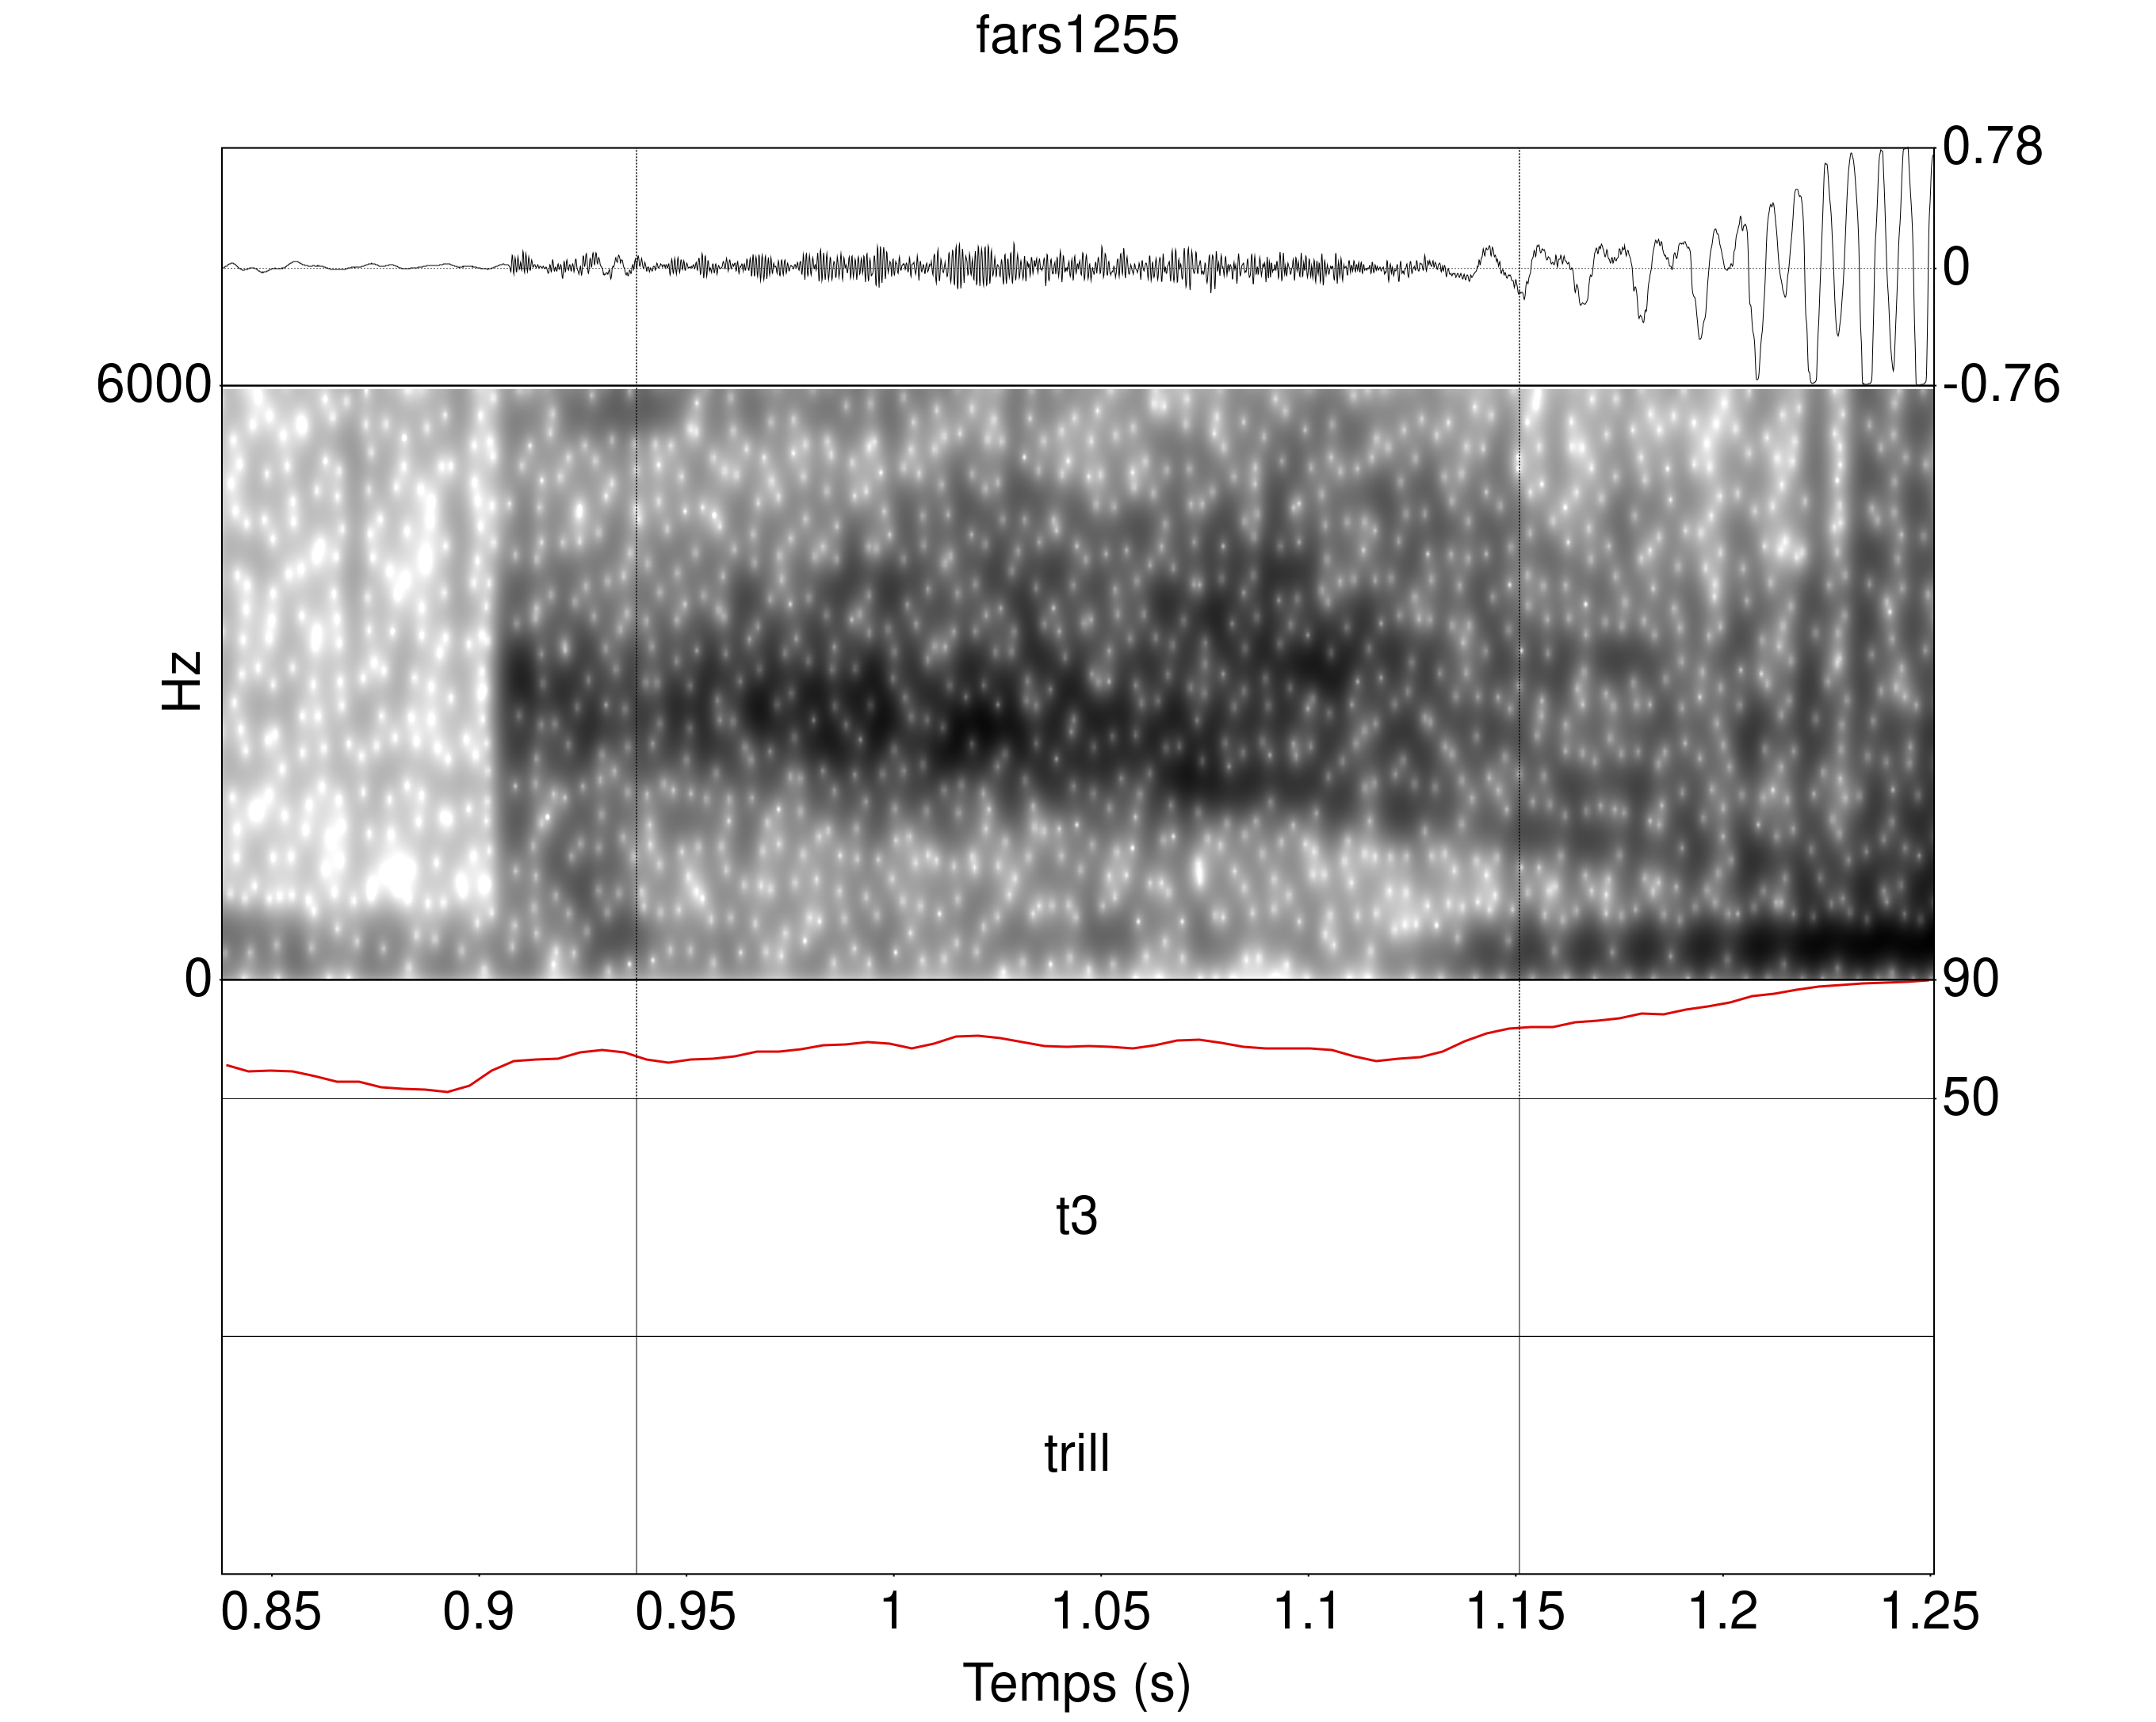
\includegraphics[width=0.8\linewidth]{substance/spectro_images/fars1255_449_2}
	\caption[Illustration de la catégorie \textg{t3}]{Illustration de la catégorie \textg{t3} dans le contexte [ˈjet ˈruzi] en farsi \glotto{fars1255}. De haut en bas, nous avons l'oscillogramme, le spectrogramme, la courbe d'intensité, un palier intervallique avec la catégorie segmentée, et un palier intervallique comprenant le label descriptif du segment d'intérêt.}
	\label{fig:fars12554492}
\end{figure}


La catégorie \textg{t4} fait référence à tout le reste, il s'agit d'une catégorie où on retrouve principalement des approximantes.\\

\begin{figure}
	\centering
	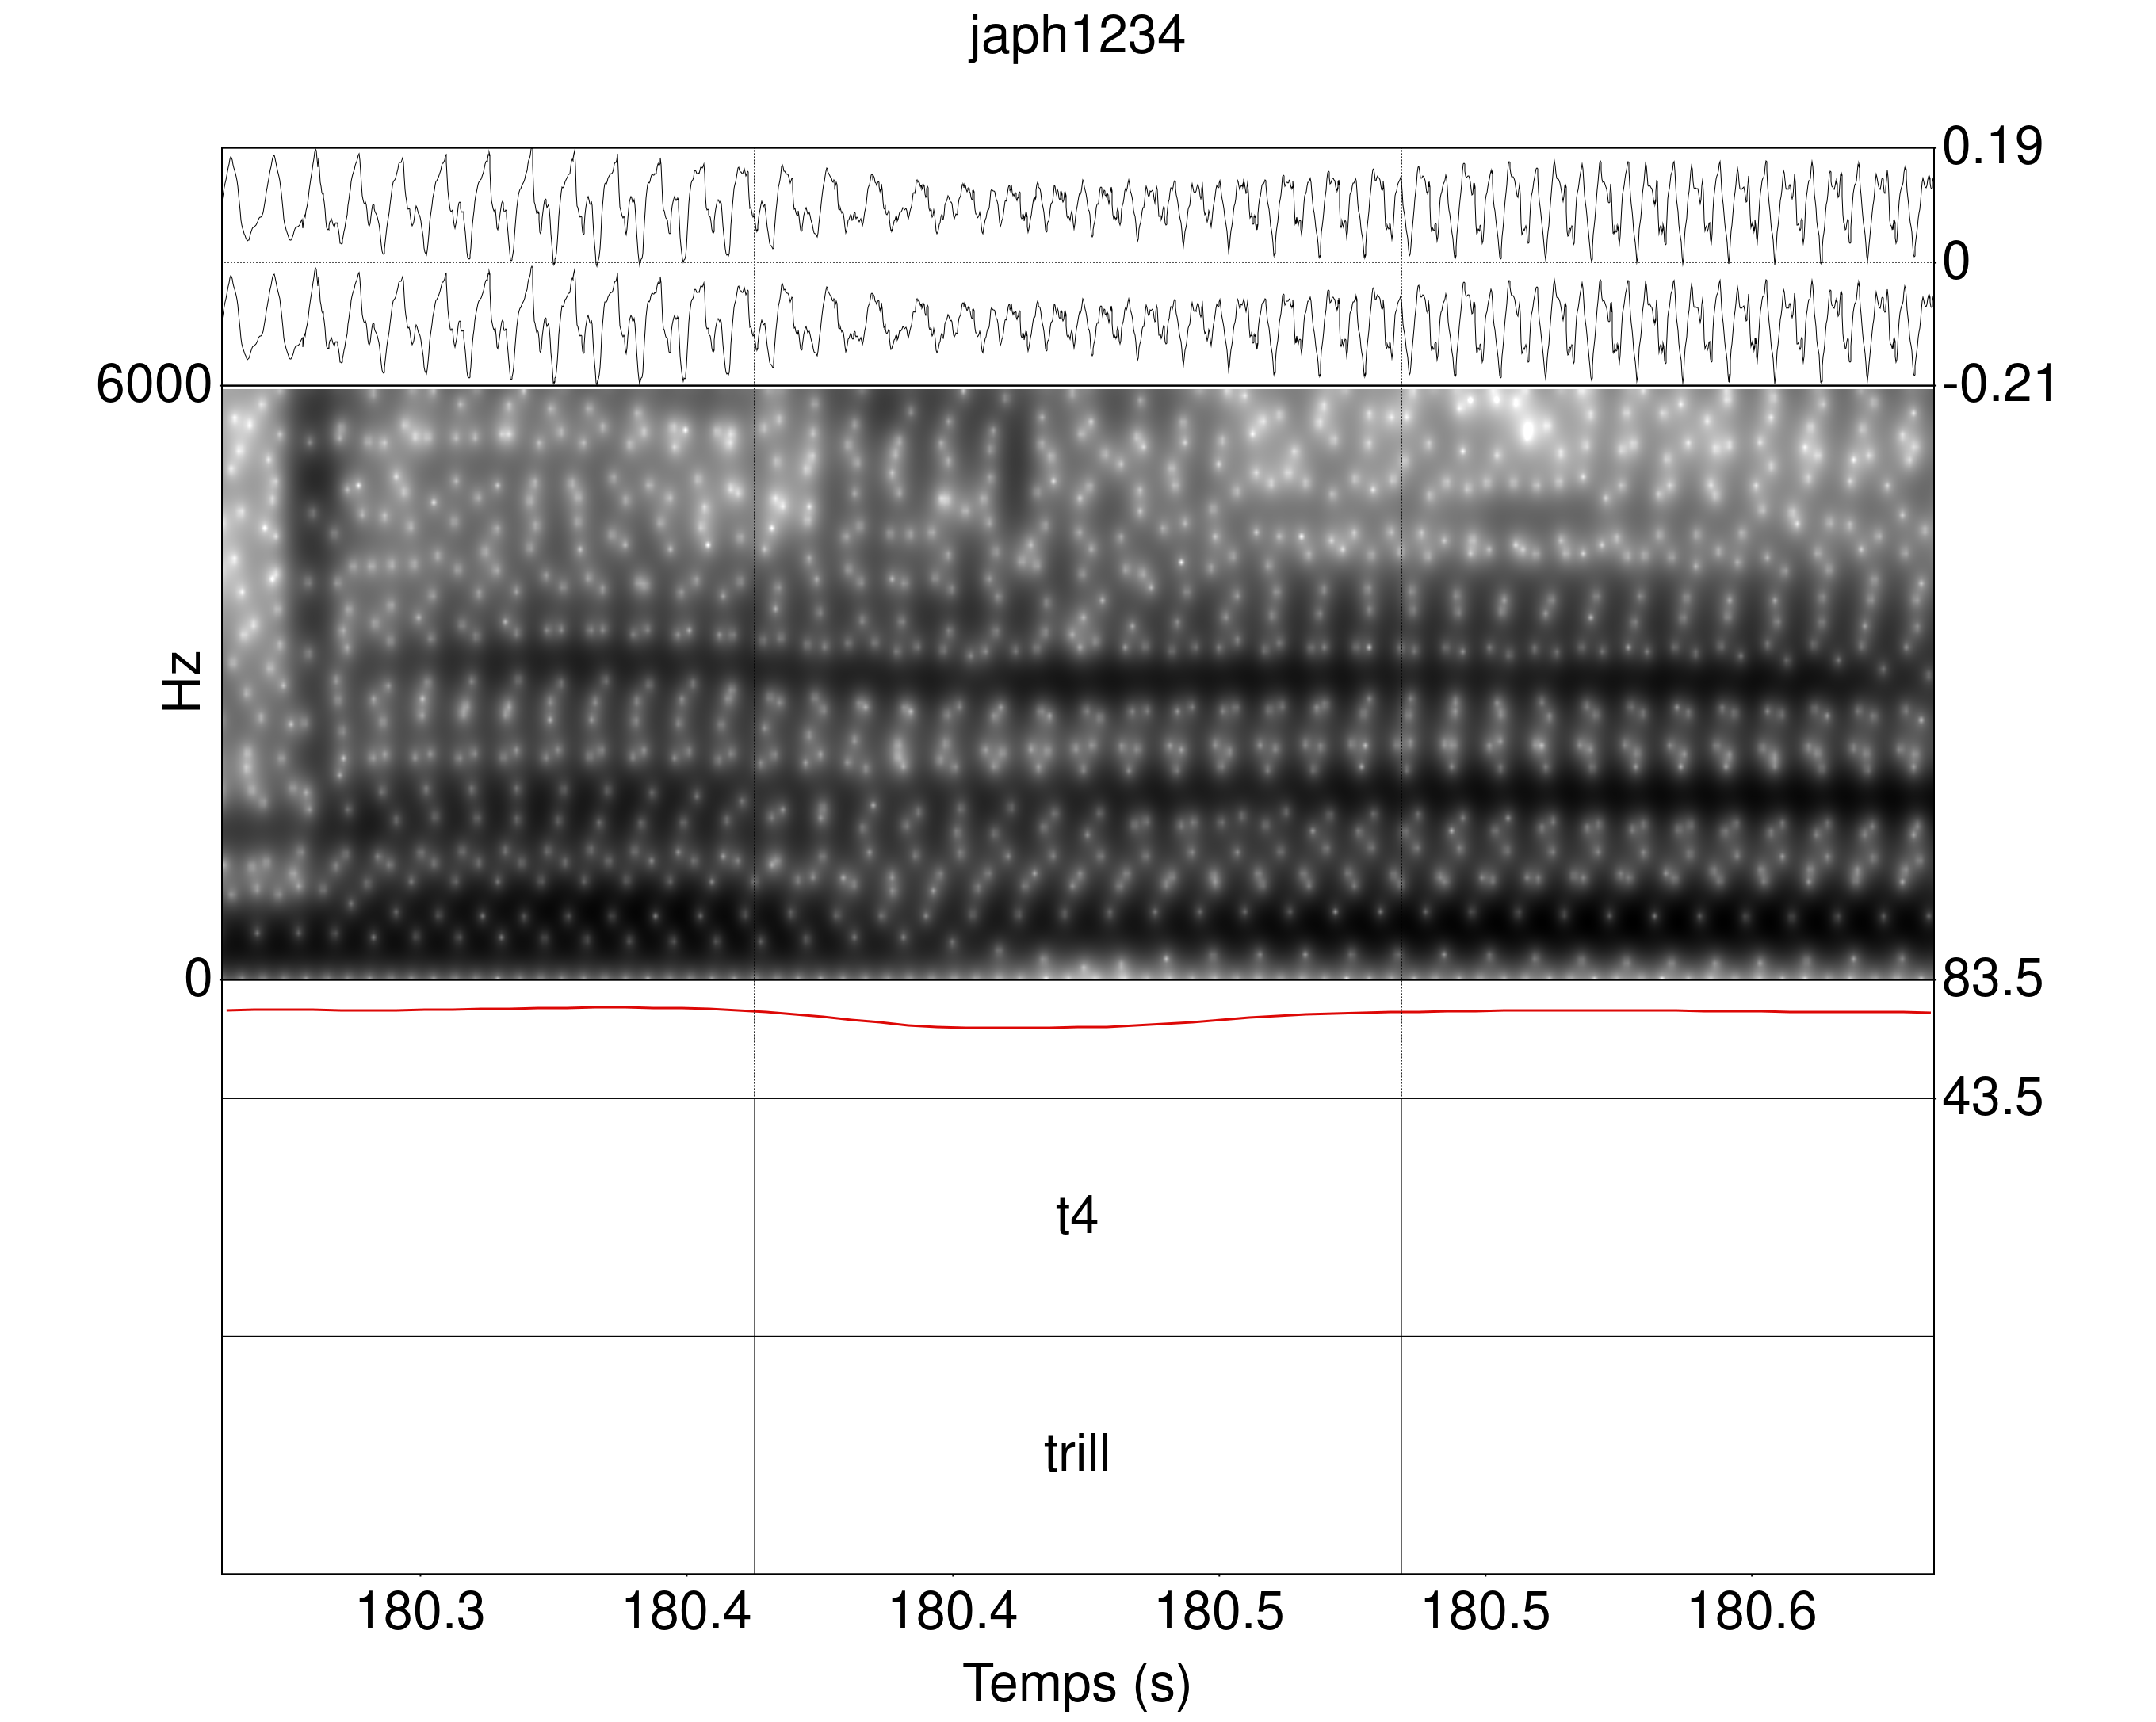
\includegraphics[width=0.8\linewidth]{substance/spectro_images/japh1234_944_70}
	\caption[Illustration de la catégorie \textg{t4}]{Illustration de la catégorie \textg{t4} dans le contexte /tɕendɤre/ en japhug \glotto{japh1234}. De haut en bas, nous avons l'oscillogramme, le spectrogramme, la courbe d'intensité, un palier intervallique avec la catégorie segmentée, et un palier intervallique comprenant le label descriptif du segment d'intérêt.}
	\label{fig:japh123494470}
\end{figure}

De plus, nous avons ajouté deux autres catégories (\autoref{fig:taus_mono}) : \textg{t5}, faisant référence à un segment avec une occlusion qui visuellement semble plus longue que celle d'un segment classé comme t1. Perceptuellement, le segment ressemble à une occlusive. La catégorie \textg{t6} fait référence à un segment avec plus de 5-6 contacts.\\

\begin{figure}
	\centering
	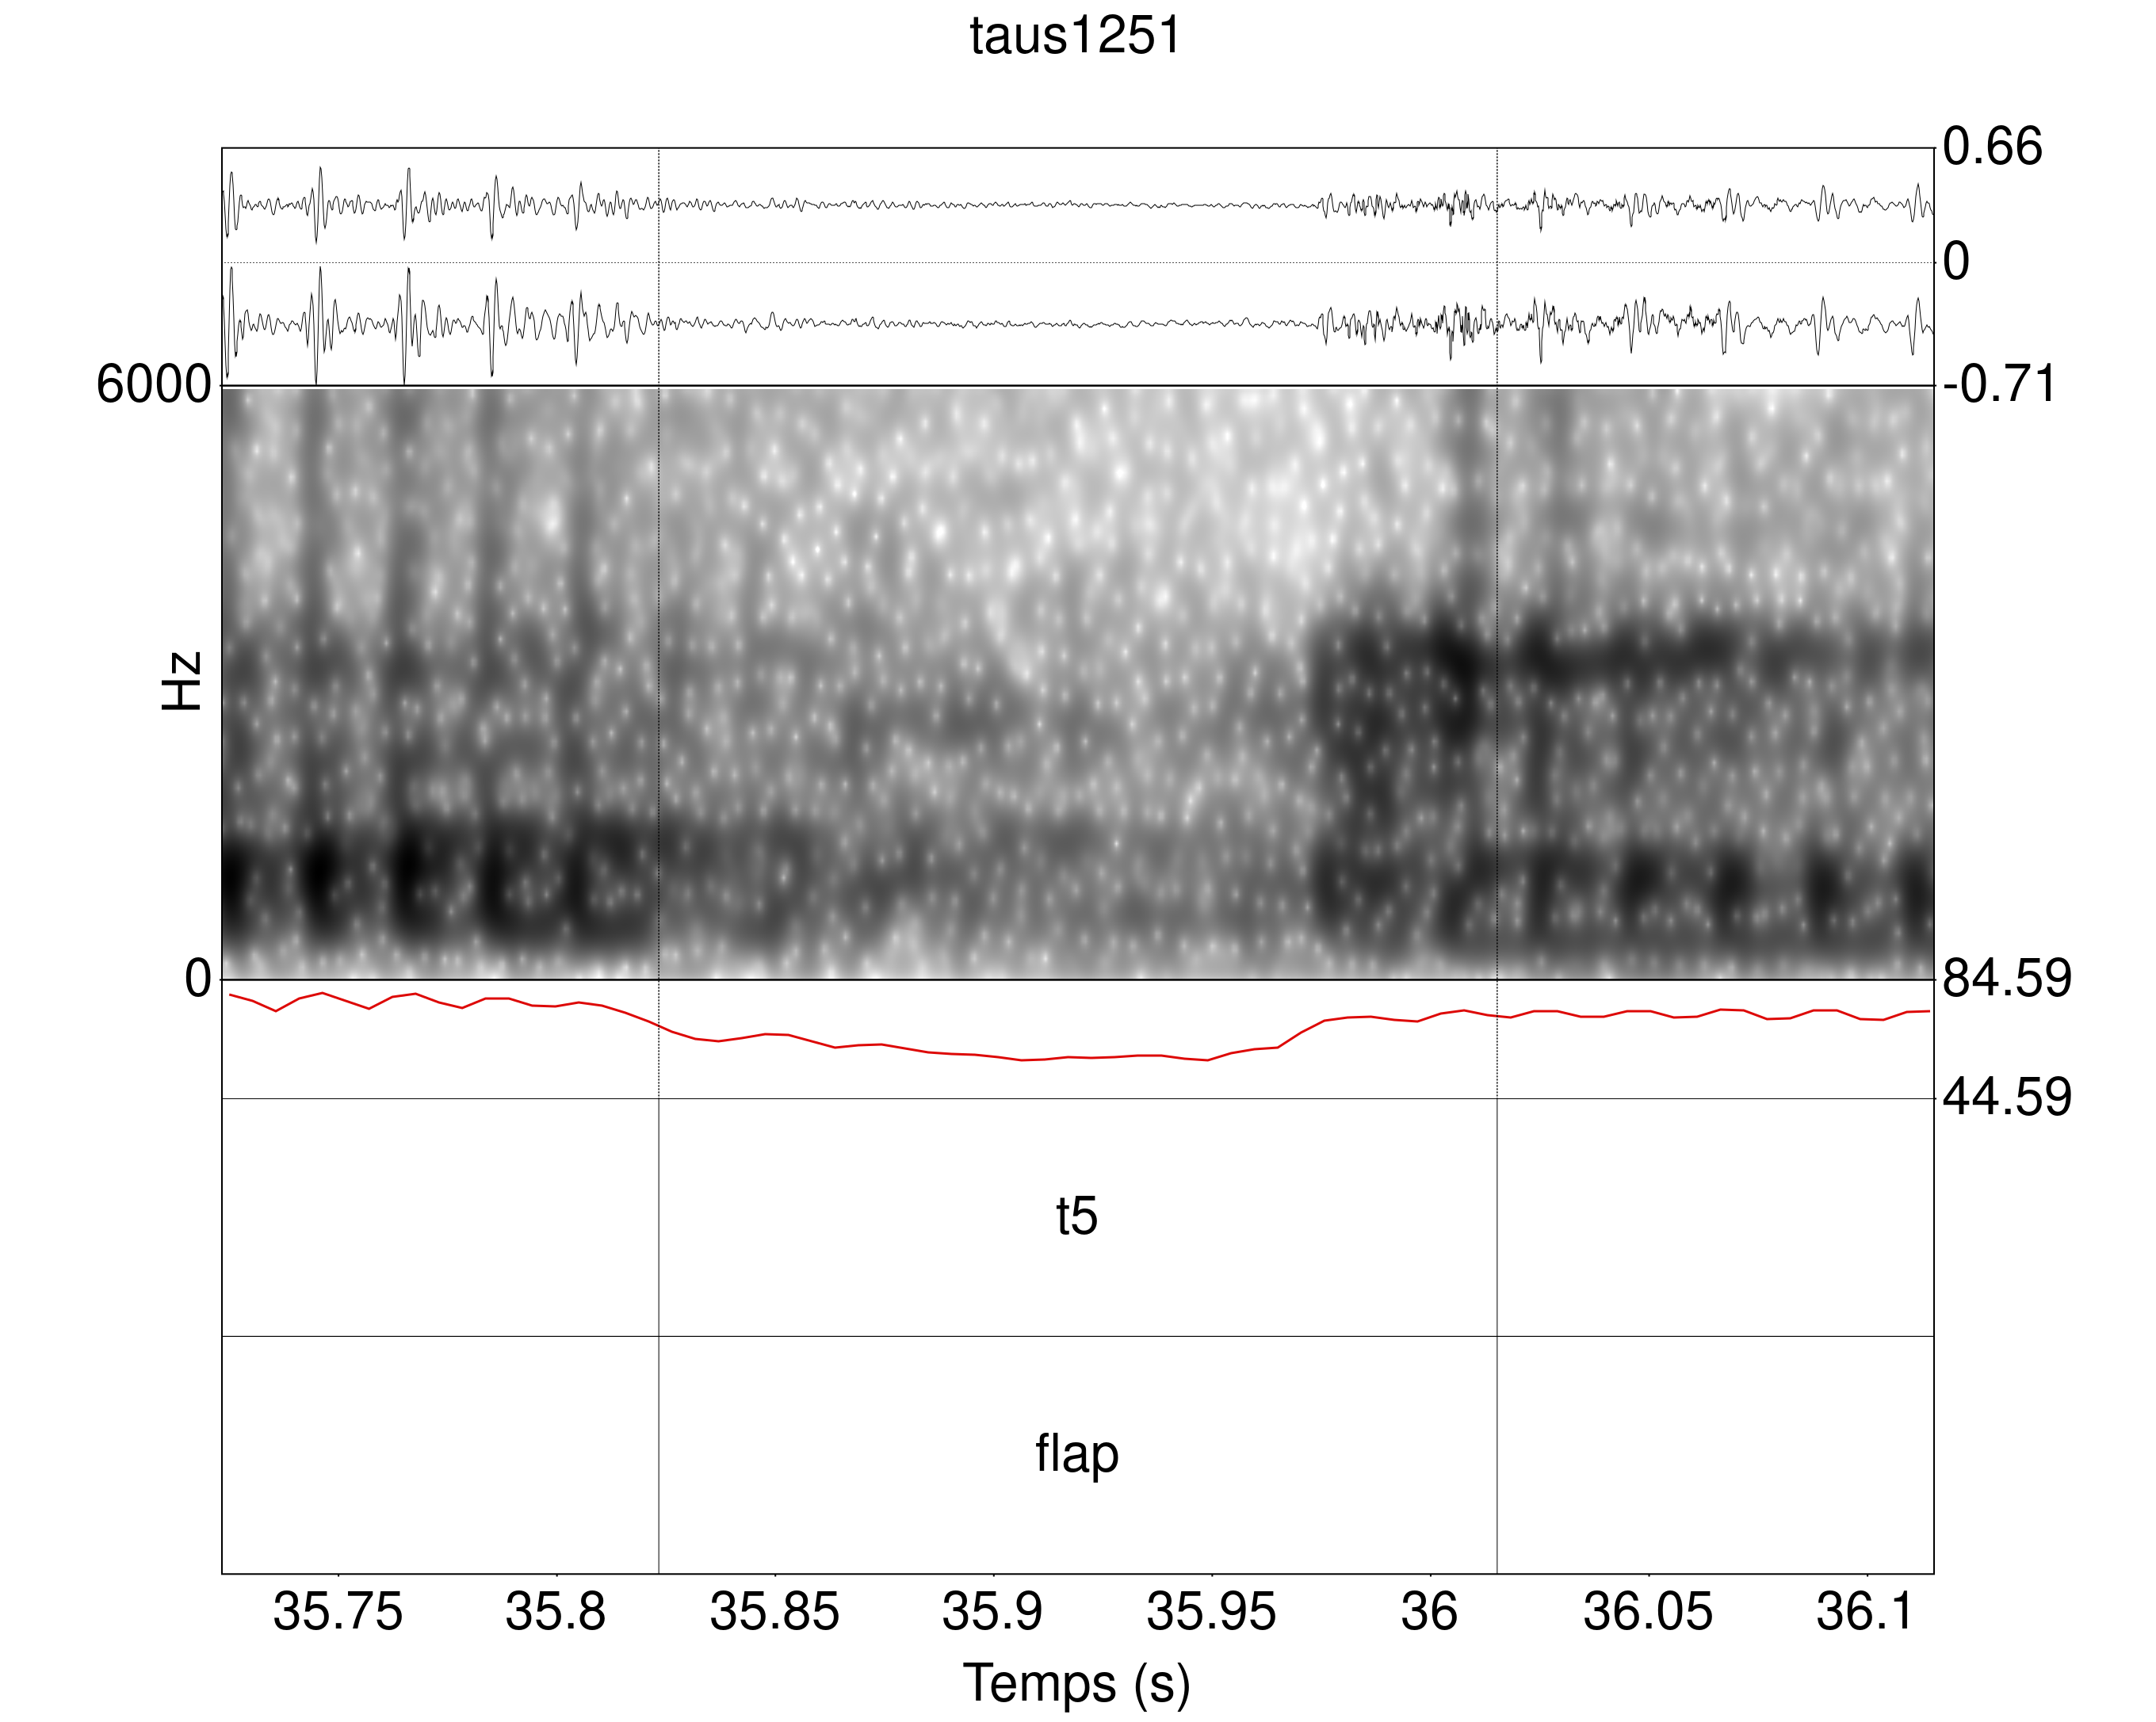
\includegraphics[width=0.45\linewidth]{substance/spectro_images/taus1251_1657_10}
	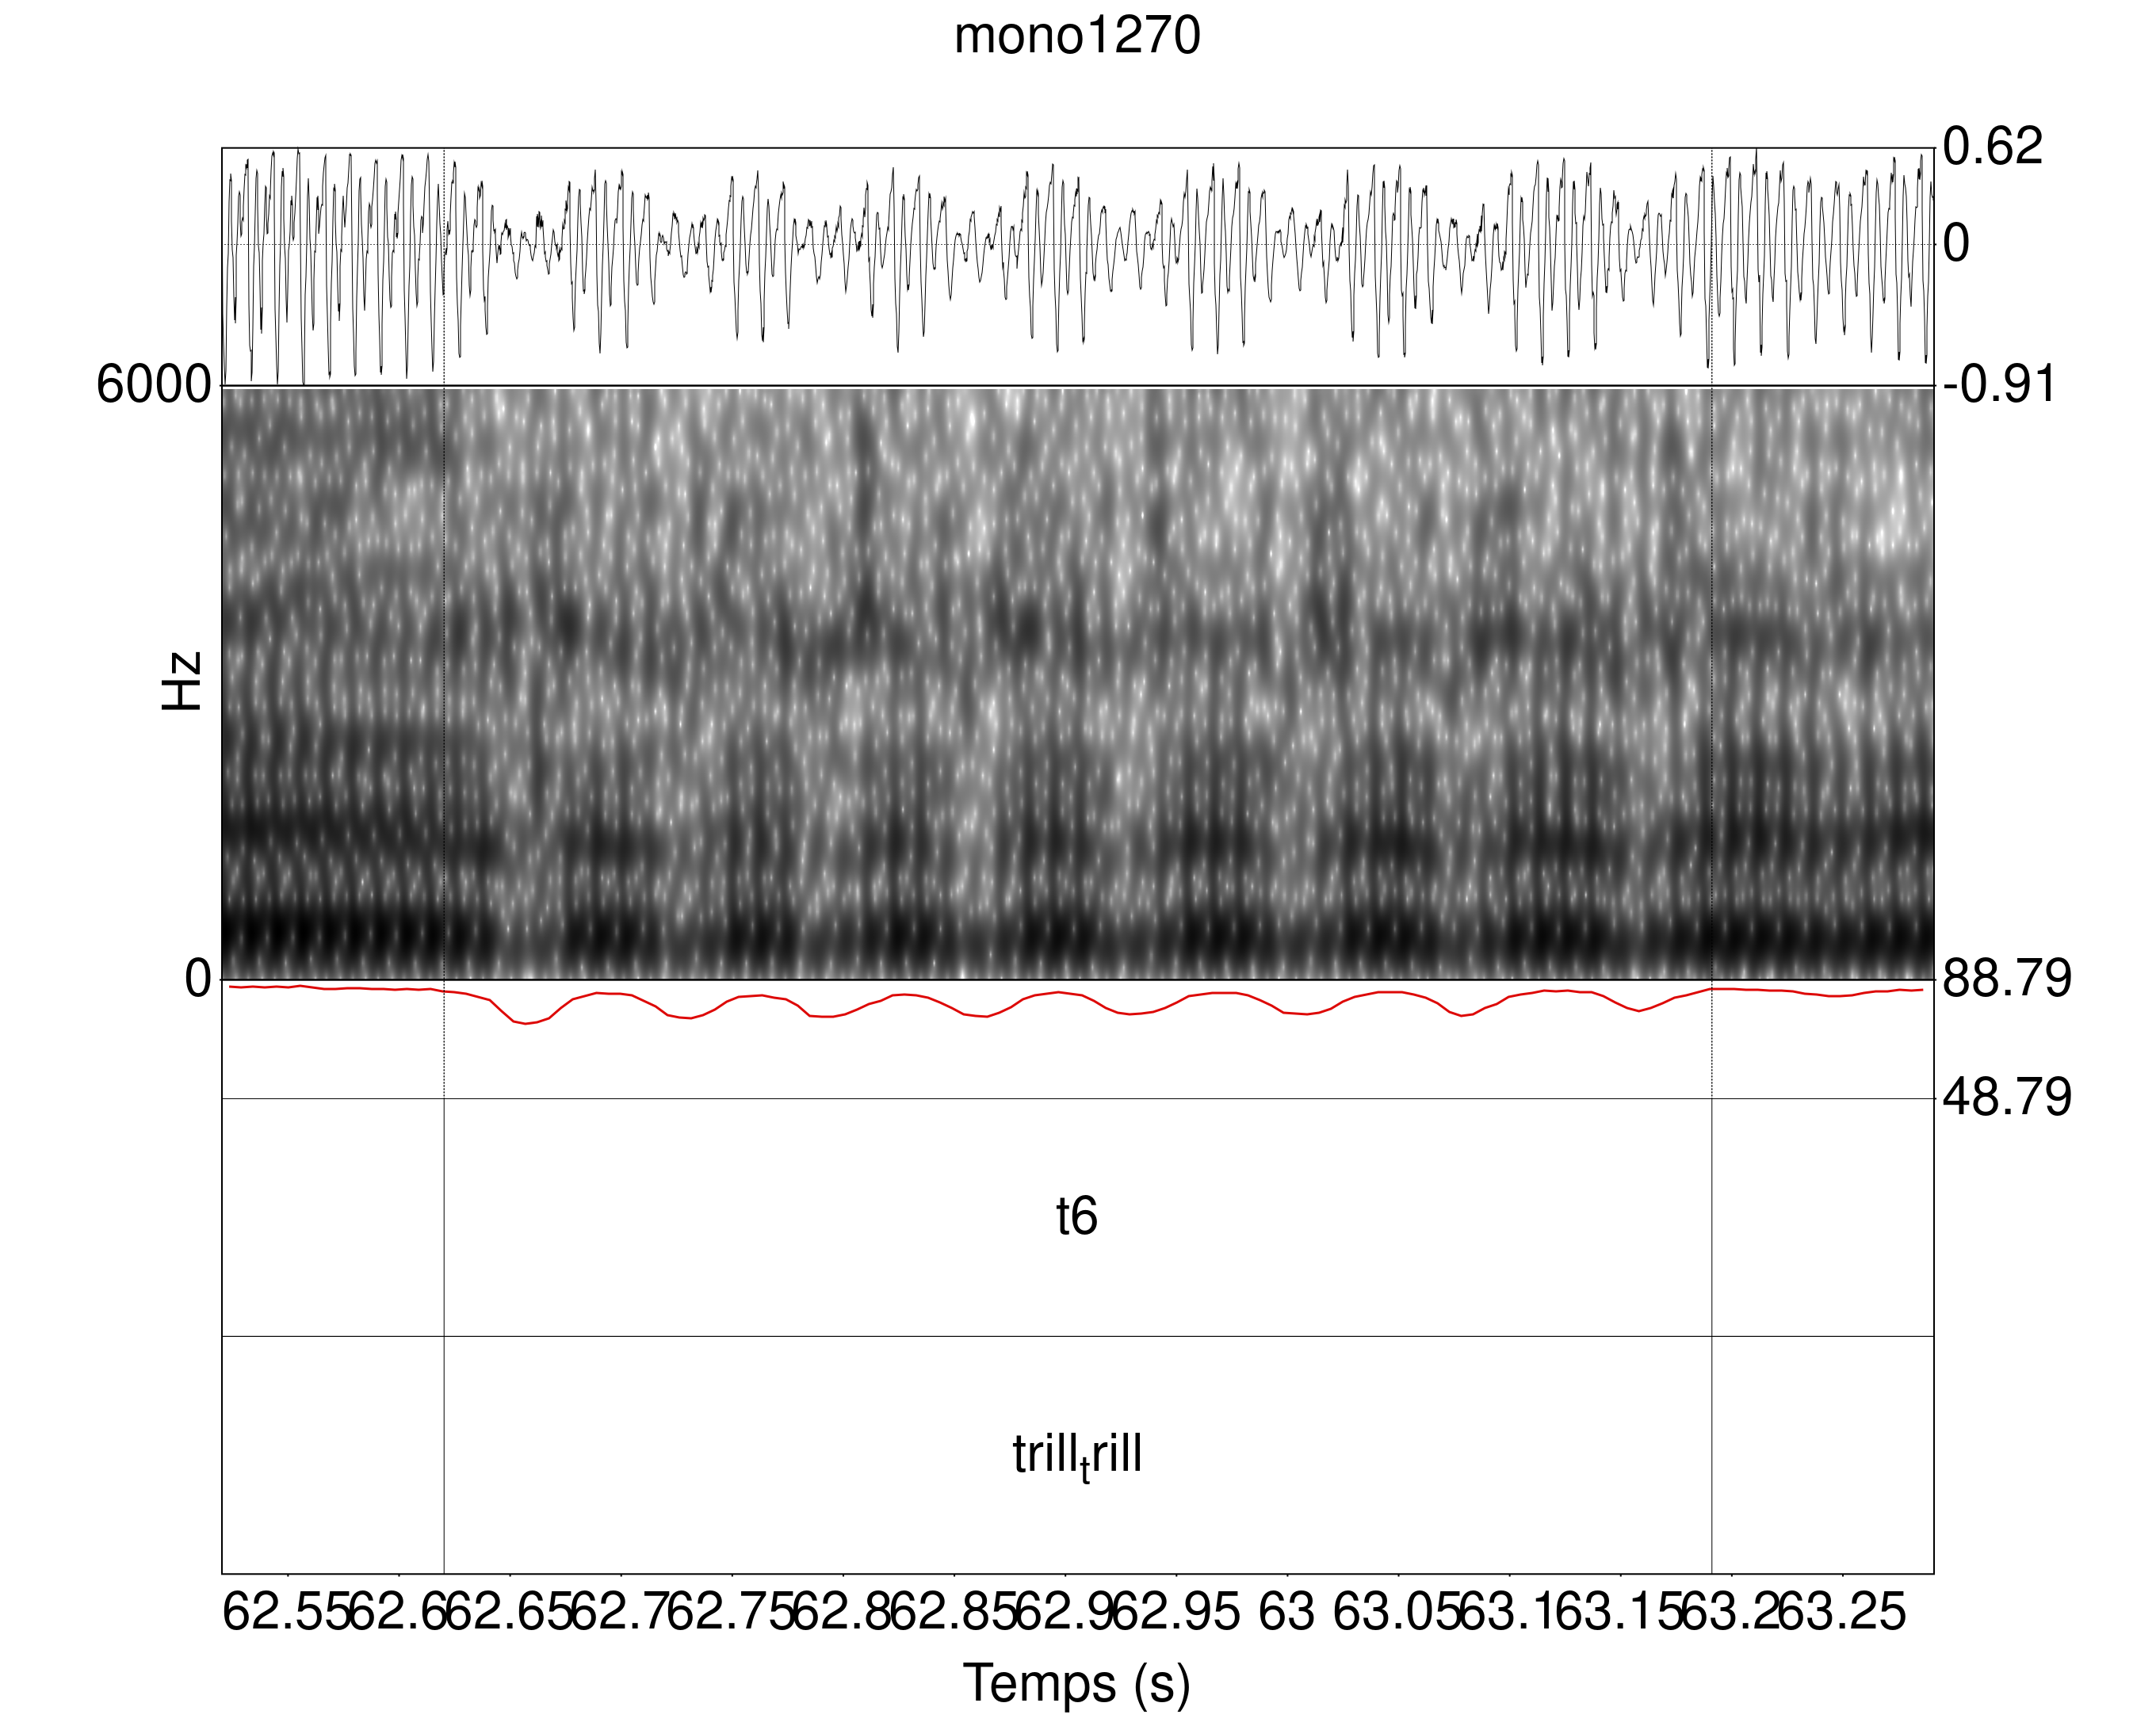
\includegraphics[width=0.45\linewidth]{substance/spectro_images/mono1270_1188_12}
	\caption[Illustrations des catégories \textg{t5} et \textg{t6}]{Illustration de la catégorie \textg{t5} dans le contexte [haˈɾuwa] en tausug (à gauche) et illustration de la catégorie \textg{t6} dans le contexte [ə́rː jìgú] <Œrrrœ yigu> en mono (à droite). De haut en bas pour chacune des illustrations, nous avons l'oscillogramme, le spectrogramme, la courbe d'intensité, un palier intervallique avec la catégorie segmentée, et un palier intervallique comprenant le label descriptif du segment d'intérêt.}
	\label{fig:taus_mono}
\end{figure}

\subsection{Résultats de la segmentation en catégories}

\begin{table}
	\centering
	%\resizebox{0.7\linewidth}{!}{\csvautobooktabular{substance/tables/table_elements_diff.csv}}
	\resizebox{\linewidth}{!}{


\begin{tabular}{p{4.5cm} l  || p{4.5cm} l}
\hline
Label descriptif	&	Fréquence	&	Label descriptif	&	Fréquence	\\
\hline
Trill	&	1117	&	Trill géminé	&	9	\\
Tap	&	434	&	Tap rétroflexe	&	6	\\
Trill/tap	&	54	&	Trill uvulaire	&	6	\\
Trill/flap	&	28	&	Trill non voisé	&	4	\\
Stop	&	22	&	Tap non voisé	&	3	\\
Tap/flap	&	22	&	Trill/fricative	&	3	\\
Flap	&	20	&	Trill rétroflexe	&	2	\\
Approximante rétroflexe	&	19	&	Trill syllabique	&	2	\\
Trill palatalisé	&	13	&	Approximante	&	1	\\
Stop non voisé	&	8	&	Liquide latérale	&	1	\\
Trill/flap rétroflexe	&	8	&	Trill glottalisé	&	1	\\

\hline
\end{tabular}
}
	\caption[Fréquence des différents labels descriptifs utilisés dans les \textit{Illustrations of the IPA} pour les rhotiques]{Fréquence des différents labels descriptifs utilisés dans les \textit{Illustrations of the IPA} pour les rhotiques.}
	\label{tab:table_descLabel}
\end{table}

La segmentation et l'annotation des différents segments se sont faites sur une période s'étalant sur trois mois. Nous nous sommes appuyés sur les transcriptions déjà établies dans les \textit{illustrations of the IPA}.
Au total, ce sont 1783 segments qui ont été segmentés et annotés pour 22 labels descriptifs (cf. \autoref{tab:table_descLabel}). Nous définissons ici le label descriptif comme la manière utilisée par les auteurs des différentes illustrations pour se référer à un segment.
Ainsi, un auteur peut parler d'un "r" comme étant, par exemple, un flap, un trill ou encore une approximante. Par défaut, les labels descriptifs référent à des segments produits au niveau alvéolaire. D'une part, nous avons les labels descriptifs appartenant au domaine de l'analyse linguistique, et de l'autre, les différentes catégories qui relèvent des motifs issus de l'interprétation du signal acoustique. Le signal acoustique motive les catégories, et non les labels descriptifs.
De plus, un segment qui ne possède qu'un label descriptif peut appartenir à plusieurs catégories en fonction de sa réalisation.\\

Nous avons fait le choix de ne pas inclure tous les labels descriptifs dans notre échantillon final. Nous n'avons gardé que les labels descriptifs des \textg{trill}, \textg{tap}, \textg{trill/tap}, \textg{trill/flap}, \textg{tap/flap} et \textg{flap} et les catégories \textg{t1}, \textg{t2}, \textg{t3} et \textg{t4}.
Notre échantillon final comporte les productions de 73 langues, soit au total 79 locuteurs et locutrices pour 1672 segments.\\


\begin{figure}
	\centering
	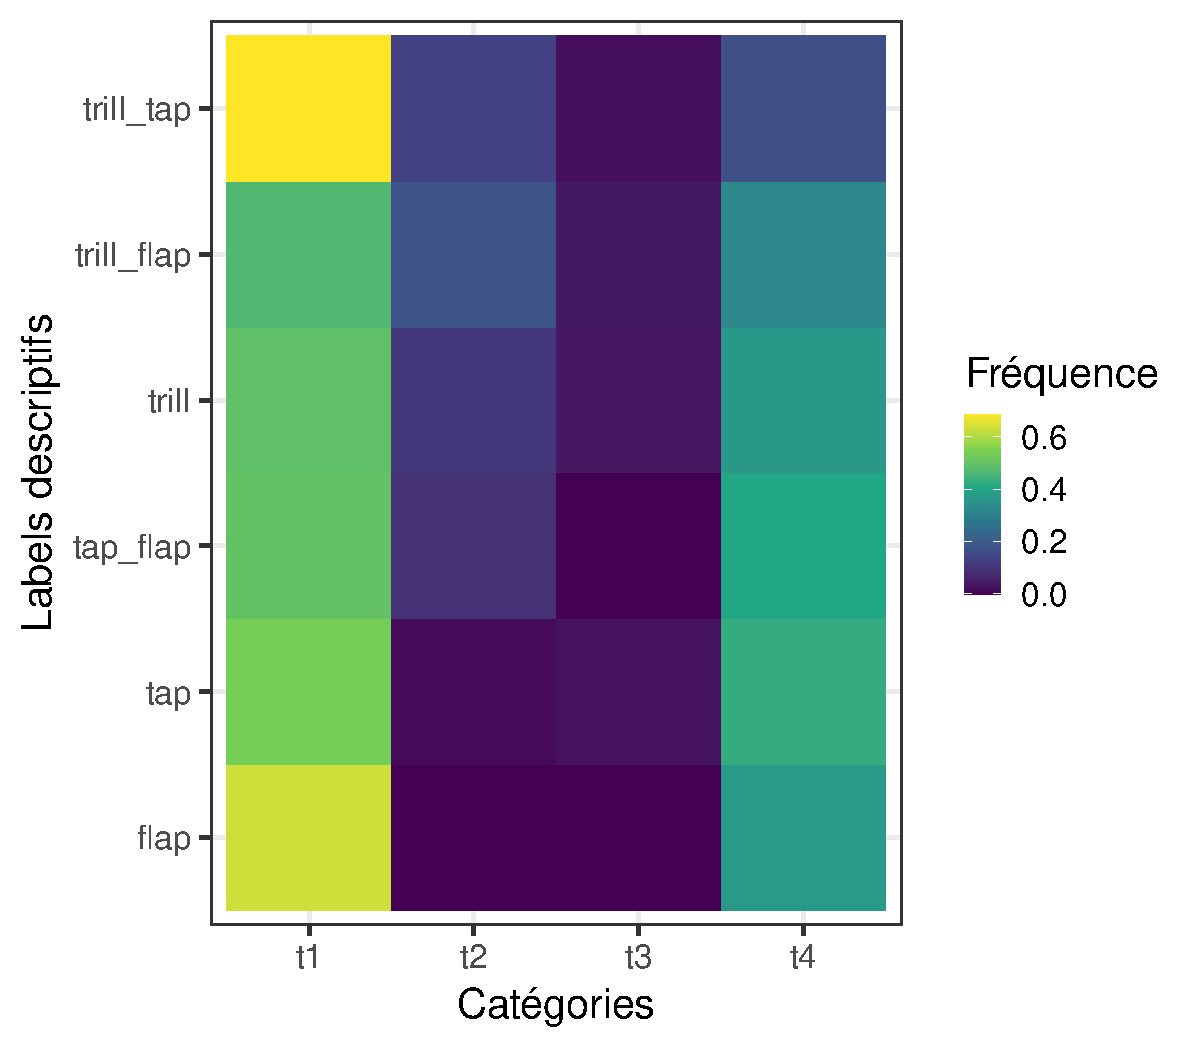
\includegraphics[width=0.45\linewidth]{substance/images/categories_full}
	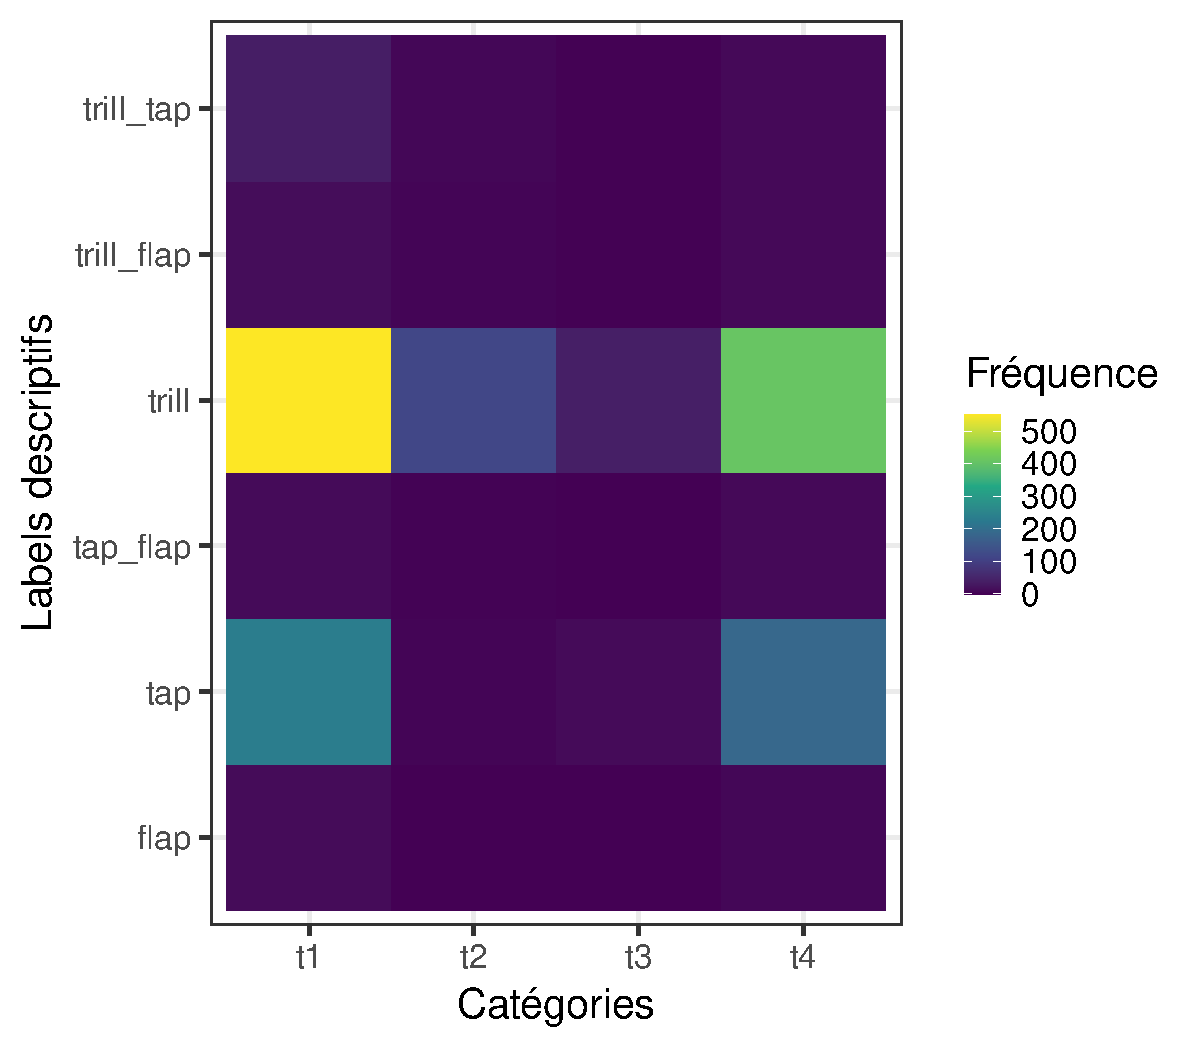
\includegraphics[width=0.45\linewidth]{substance/images/categories_full_freqabs}
	\caption[Fréquences des différentes catégories en fonction des labels descriptifs]{Fréquences relatives (à gauche) et fréquences absolues (à droite) des différentes catégories en fonction des labels descriptifs. Les fréquences sont calculées par ligne. Plus une case est jaune, plus la catégorie associée à un label descriptif est fréquente. Plus une case est violette, moins la catégorie associée à un label descriptif est fréquente.}
	\label{fig:categoriesfull}
\end{figure}

Lorsqu'on regarde les labels descriptifs, les trills sont les segments les plus fréquents dans nos données. Les trills représentent 67\% de toutes les rhotiques segmentées. Les taps représentent 26\% des données. Les trills/taps, trills/flaps, taps/flaps et flaps se partagent les 7\% restants.
La plupart des segments ont été catégorisés comme des \textg{t1} et des \textg{t4} (\autoref{fig:categoriesfull}). La catégorie \textg{t2} n'est jamais la plus fréquente même dans les cas où le label descriptif est \textg{trill}, autrement dit, un motif acoustique avec au moins deux occlusions n'est jamais le motif le plus fréquent dans les segments identifiés comme \textit{trill} par les auteurs des illustrations.\\

Dans la partie qui suit, nous allons nous intéresser à la variation entre les langues, en contrôlant le label descriptif utilisé par les auteurs des illustrations. Autrement dit, comme chaque langue est représentée par un locuteur ou une locutrice, nous allons observer la variation inter-locuteur.\\


Nous nous intéressons dans un premier temps au trill. En \autoref{fig:variationtrill} nous pouvons observer les données pour les 65 locuteurs/trices de langues où on retrouve des trills.
Parmi ces personnes enregistrées, seulement six ont réalisé au moins 50\% de leurs segments labellisés \textg{trill} comme des \textg{t2}, et ce chiffre augmente à huit pour les personnes en ayant réalisés au moins 40\%.
En \autoref{fig:galicastmalotswa} nous présentons les oscillogrammes, spectrogrammes et segmentations avec annotations de six de ces huit personnes. Il est intéressant de souligner que l'espagnol d'Argentine \glotto{amer1254}, le castillan \glotto{cast1244}, l'amharique \glotto{amha1245}, le galicien \glotto{gali1258} et le madurais \glotto{nucl1460} contrastent deux rhotiques dont un trill.
De plus, hormis le madurais \glotto{nucl1460} et le tamambo \glotto{malo1243}, les comptes de \textg{t2} sont inférieurs ou égaux à 3, mettant en évidence un faible nombre de productions total.
Si on regarde les fréquences absolues, 34 locuteurs/rices ont au moins un \textg{t2} comme réalisation de trills avec une moyenne à 3,44 et une médiane de 2,5 \textg{t2}.
Ainsi, 31 locuteurs/trices n'ont jamais réalisé de \textg{t2} dans leur production des trills, et seule la moitié des locuteurs/trices ont produit un \textg{t2} au moins une fois. Ce n'est donc pas parce qu'un segment est labellisé comme un trill qu'il sera réalisé comme un \textg{t2}. En outre, nous pouvons nous demander si dans une tâche de lecture de mots, ces locuteurs/trices, ne produisant pas de \textg{t2} ici, produiraient des \textg{t2}.\\


\begin{figure}
	\centering
	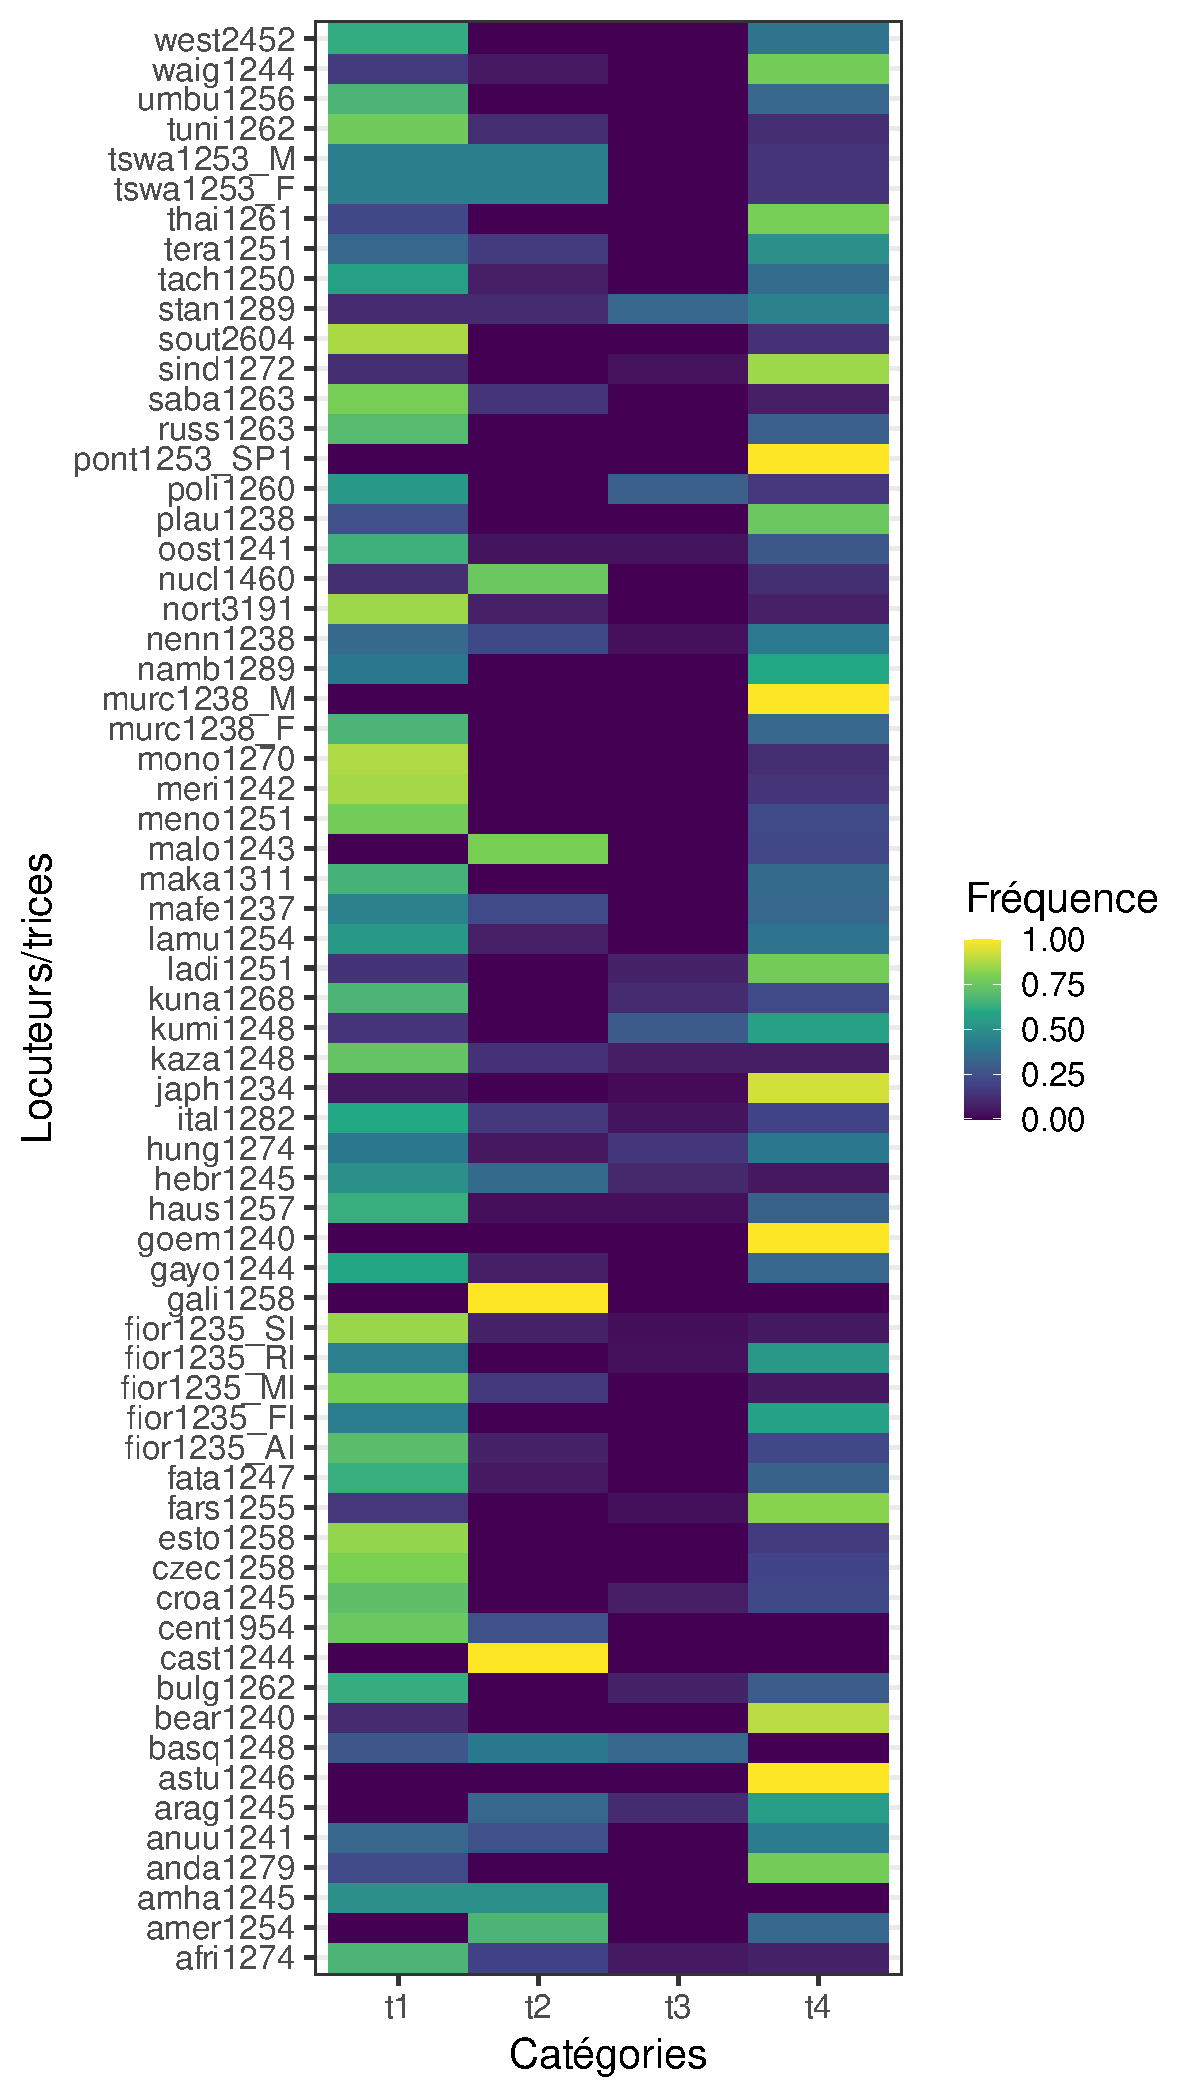
\includegraphics[width=0.45\linewidth]{substance/images/variation_trill}
	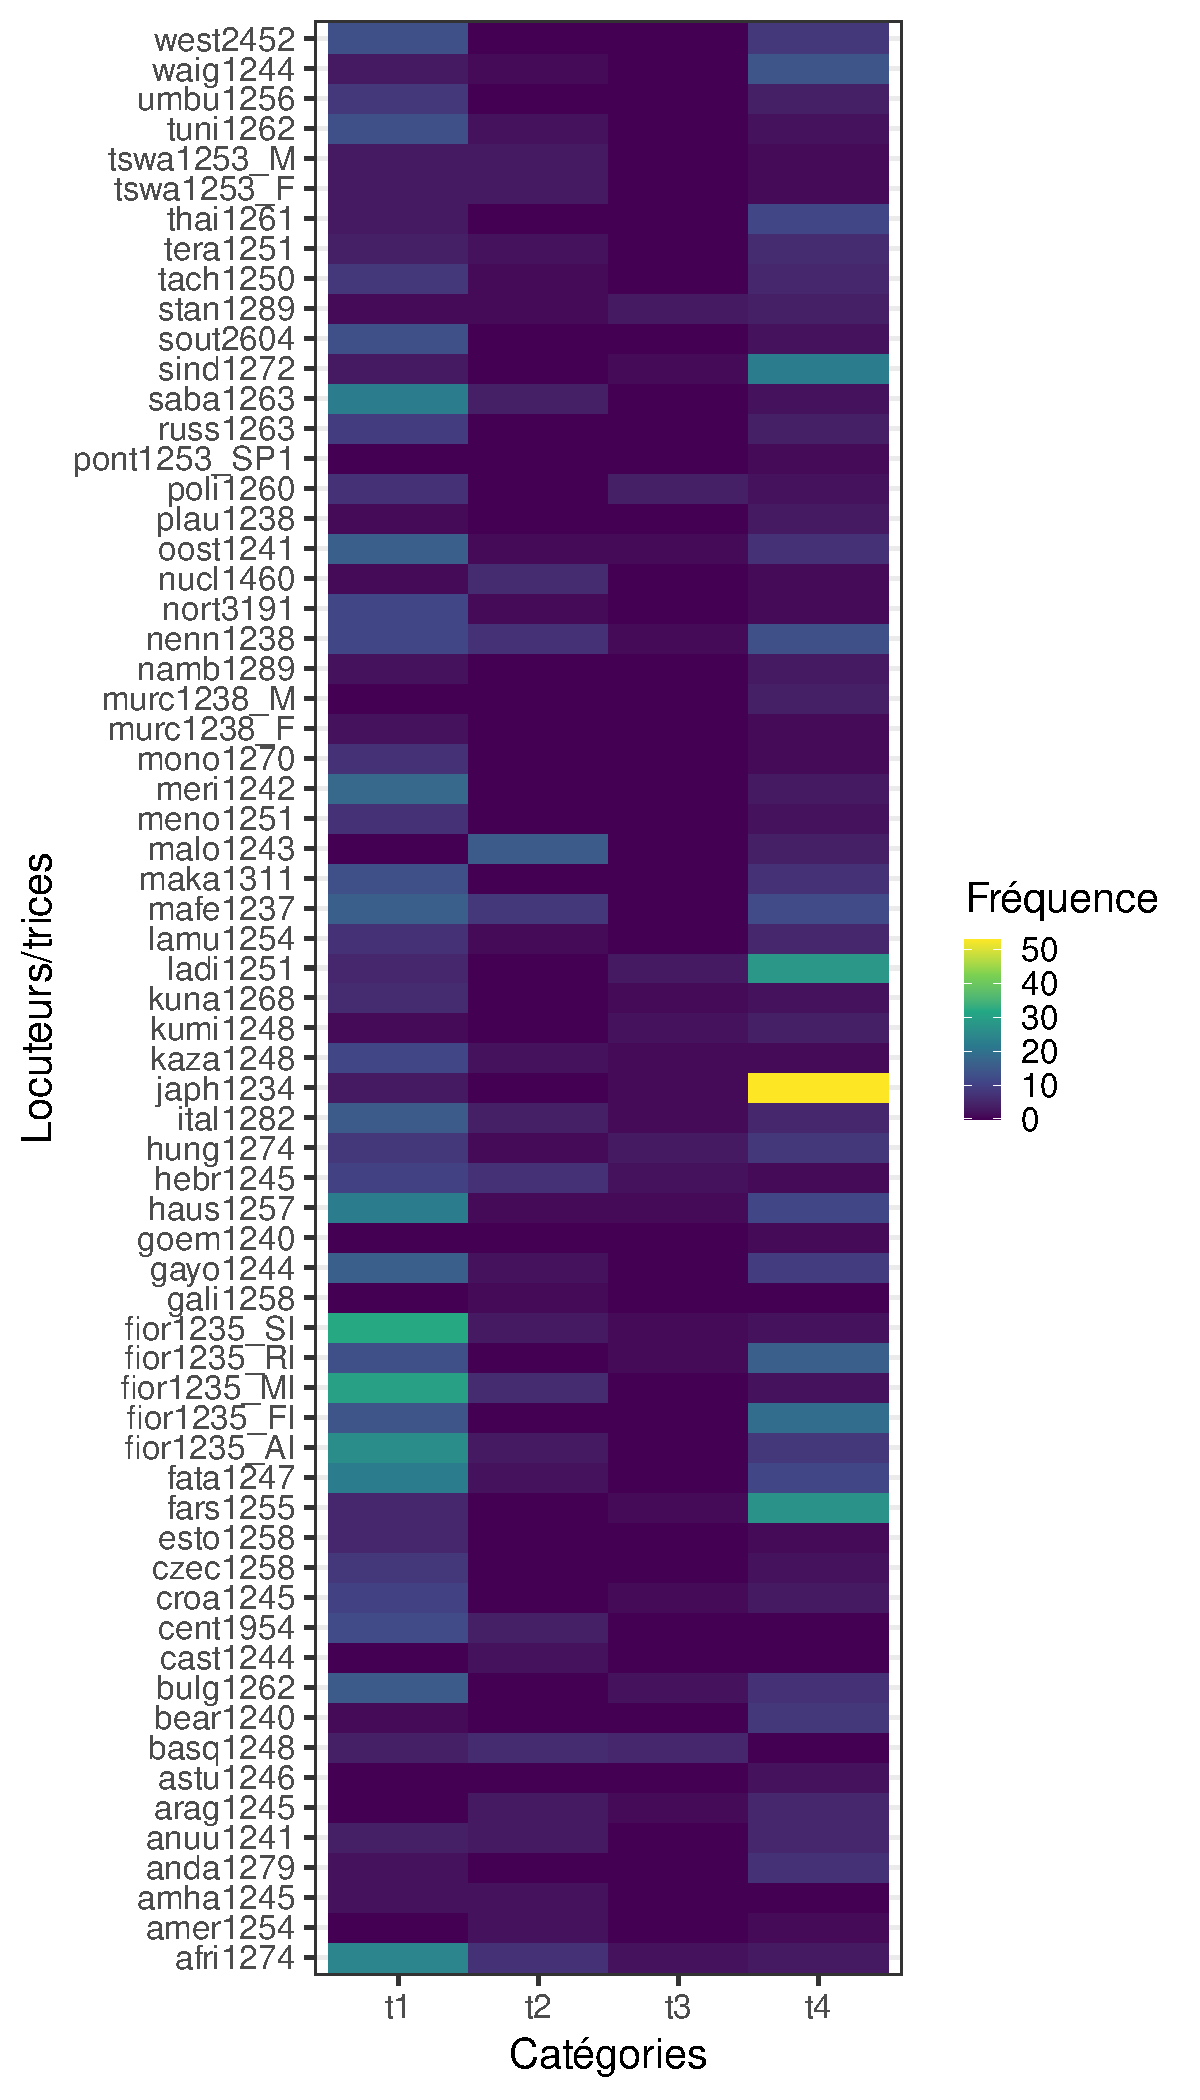
\includegraphics[width=0.45\linewidth]{substance/images/variation_trill_abs}
	\caption[Fréquences des différentes catégories illustrant la variation pour les segments ayant été catégorisés comme des \textg{trill}]{Fréquences relatives (à gauche) et absolues (à droite) des différentes catégories illustrant la variation pour les segments ayant été catégorisés par les auteurs des illustrations comme des \textg{trill}. Les fréquences sont calculées par ligne. Une case jaune est associée à une haute fréquence, cela veut dire que le/la locuteur/trice tend à produire une seule catégorie. Une case violette est associée à une catégorie non produite par le/la locuteur/trice.}
	\label{fig:variationtrill}
\end{figure}


\begin{figure}
	\centering
	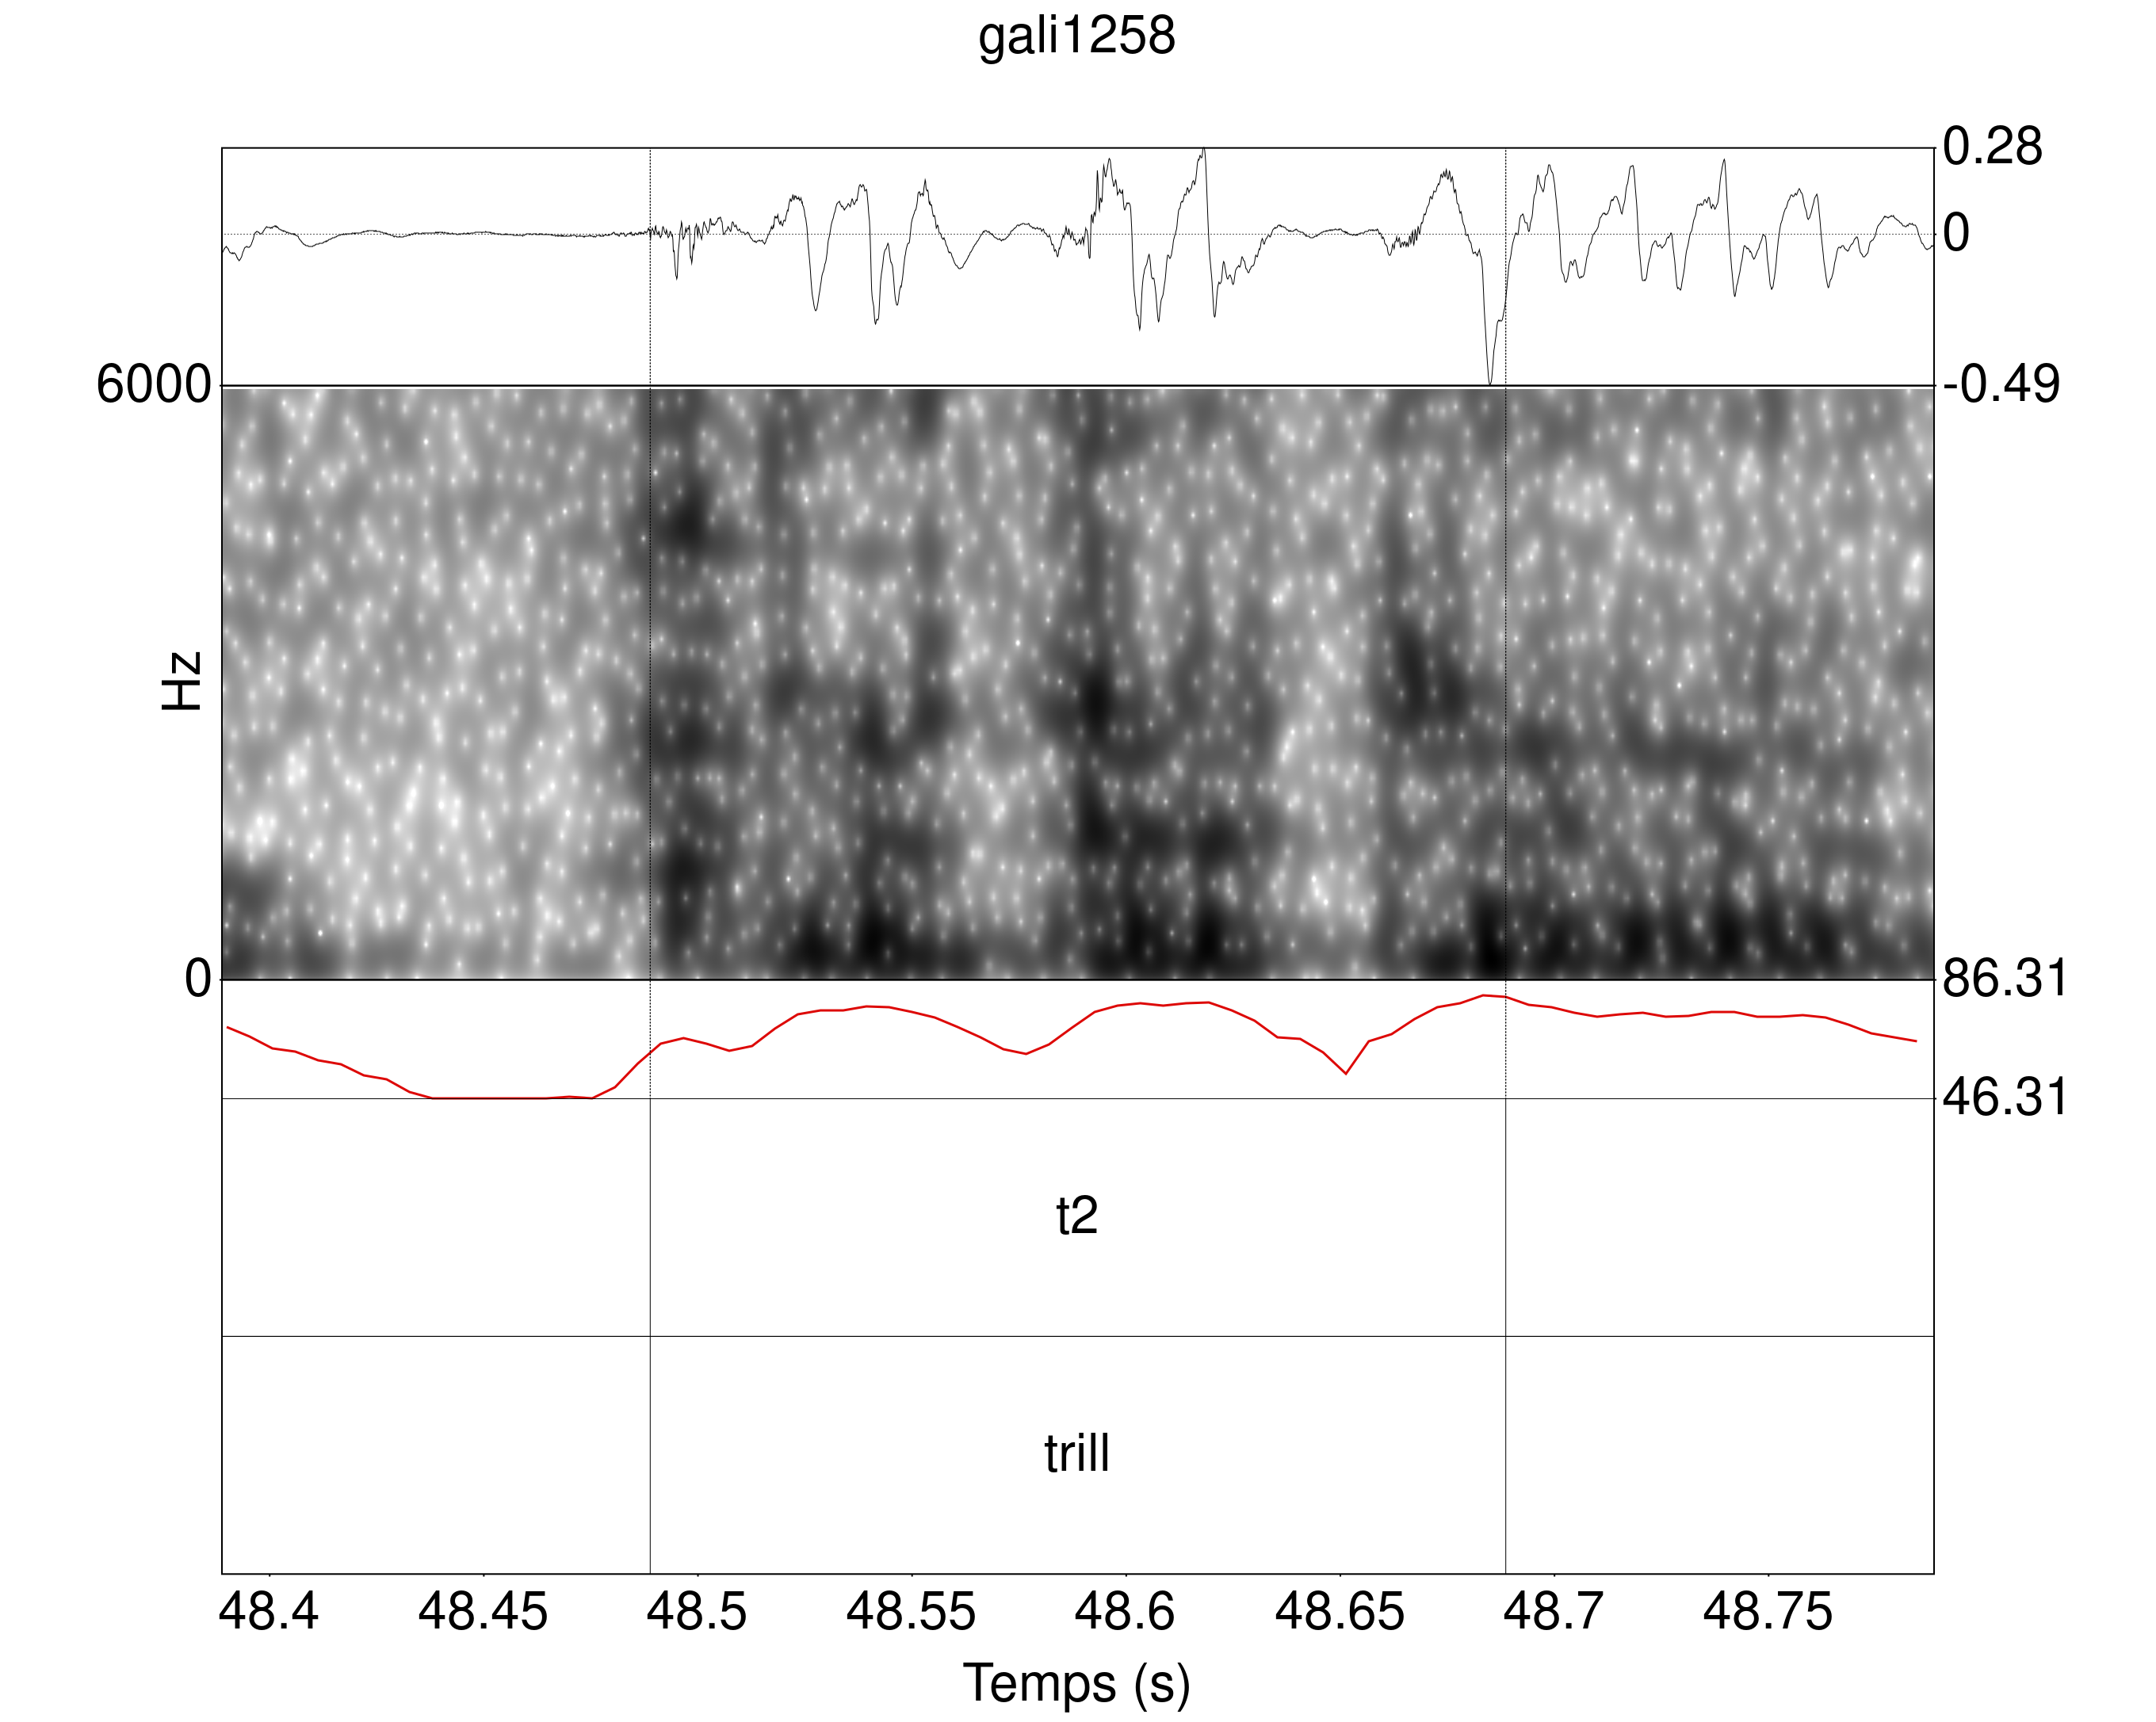
\includegraphics[width=0.45\linewidth]{substance/spectro_images/gali1258_718_48}
	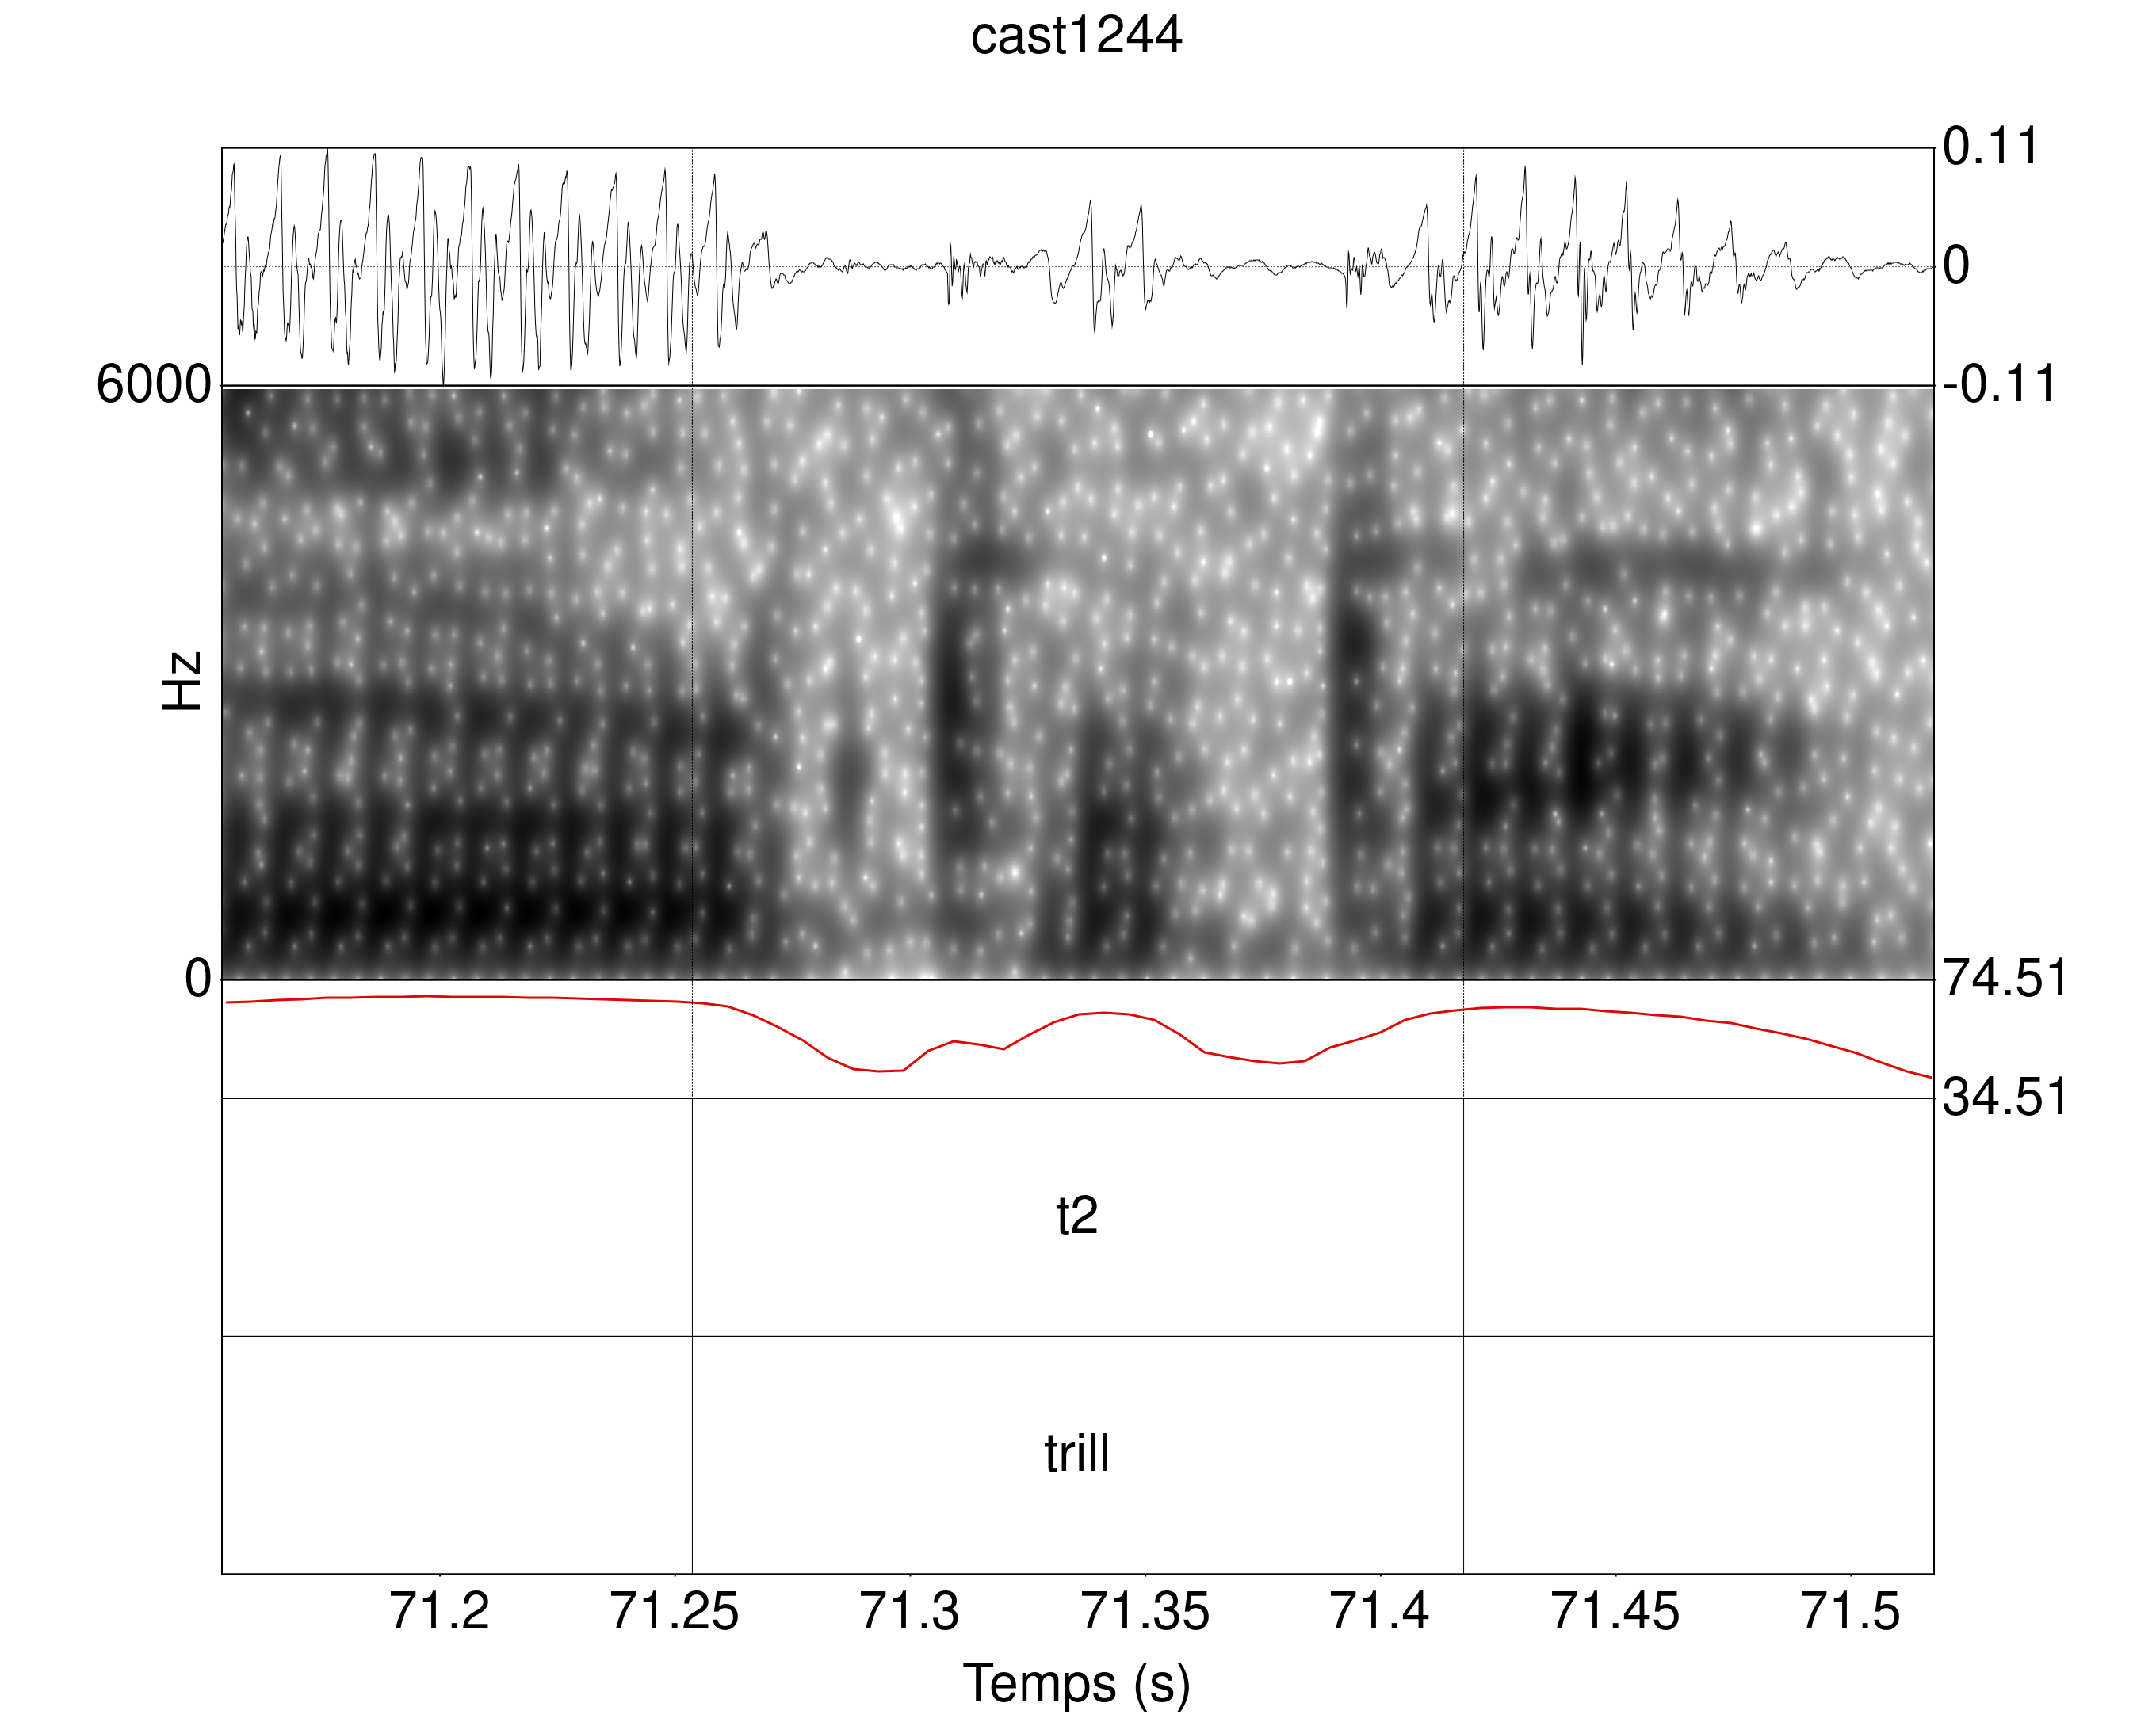
\includegraphics[width=0.45\linewidth]{substance/spectro_images/cast1244_354_66}
	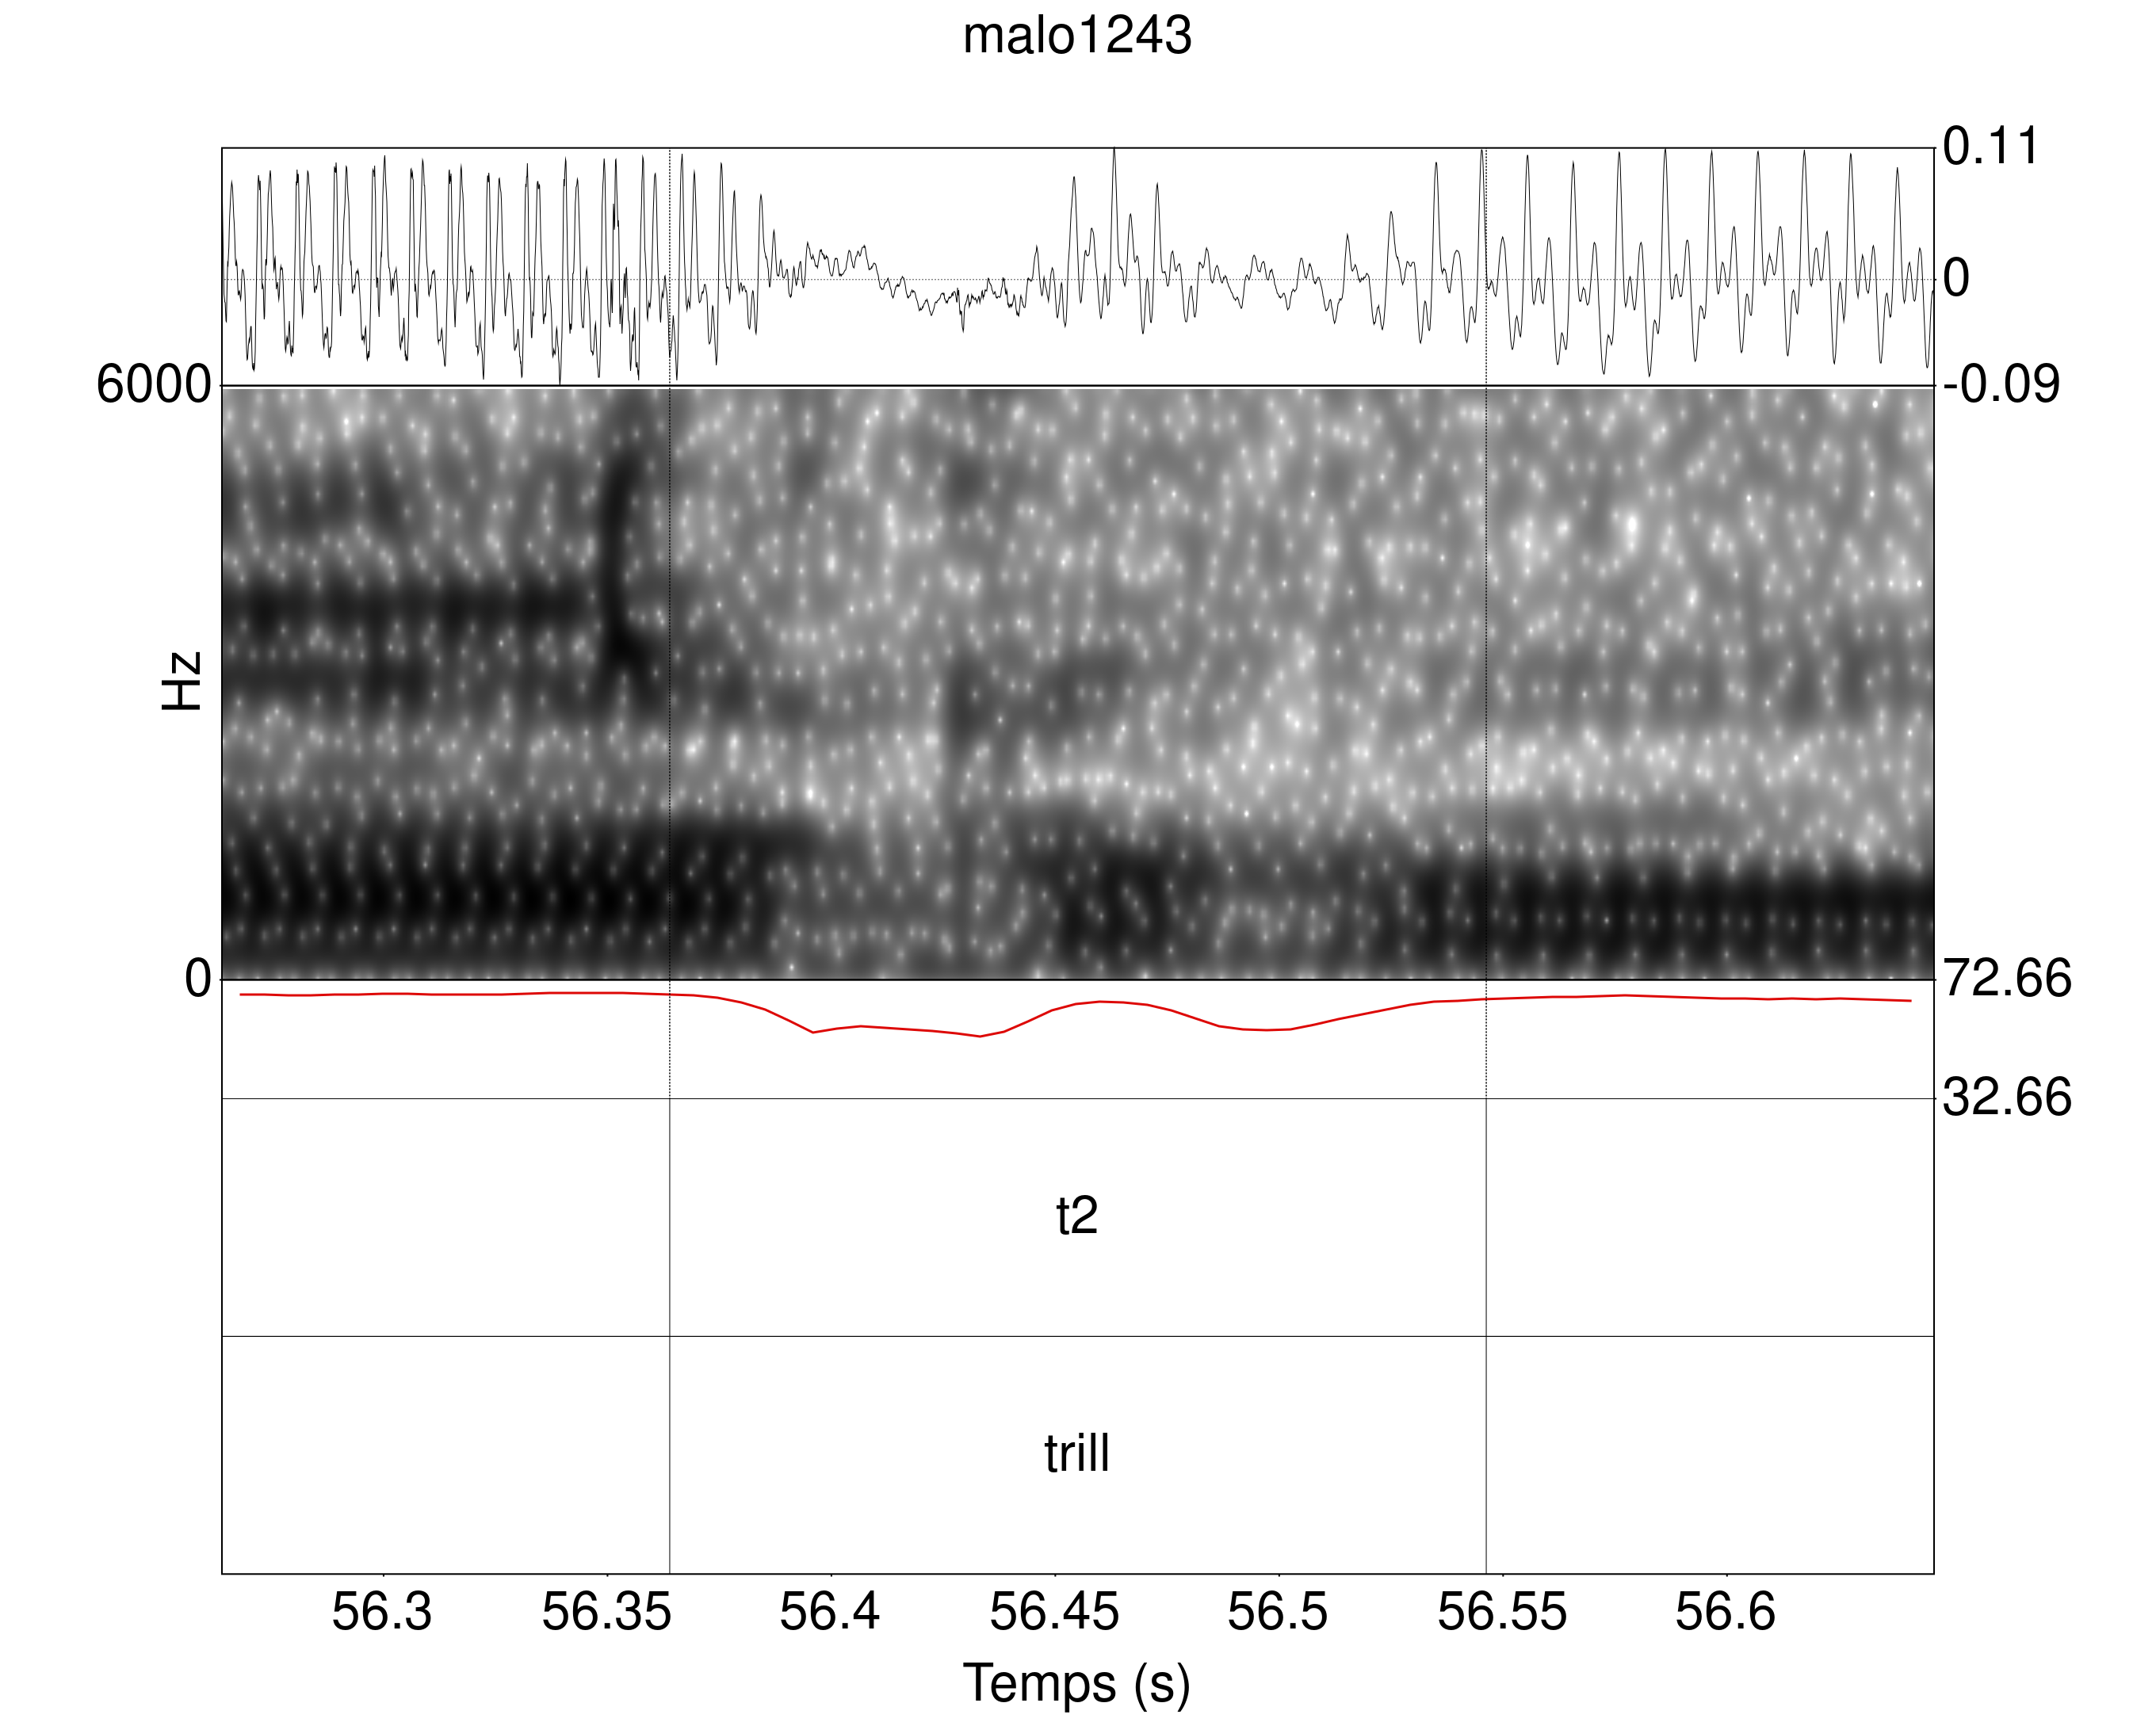
\includegraphics[width=0.45\linewidth]{substance/spectro_images/malo1243_1132_28}
	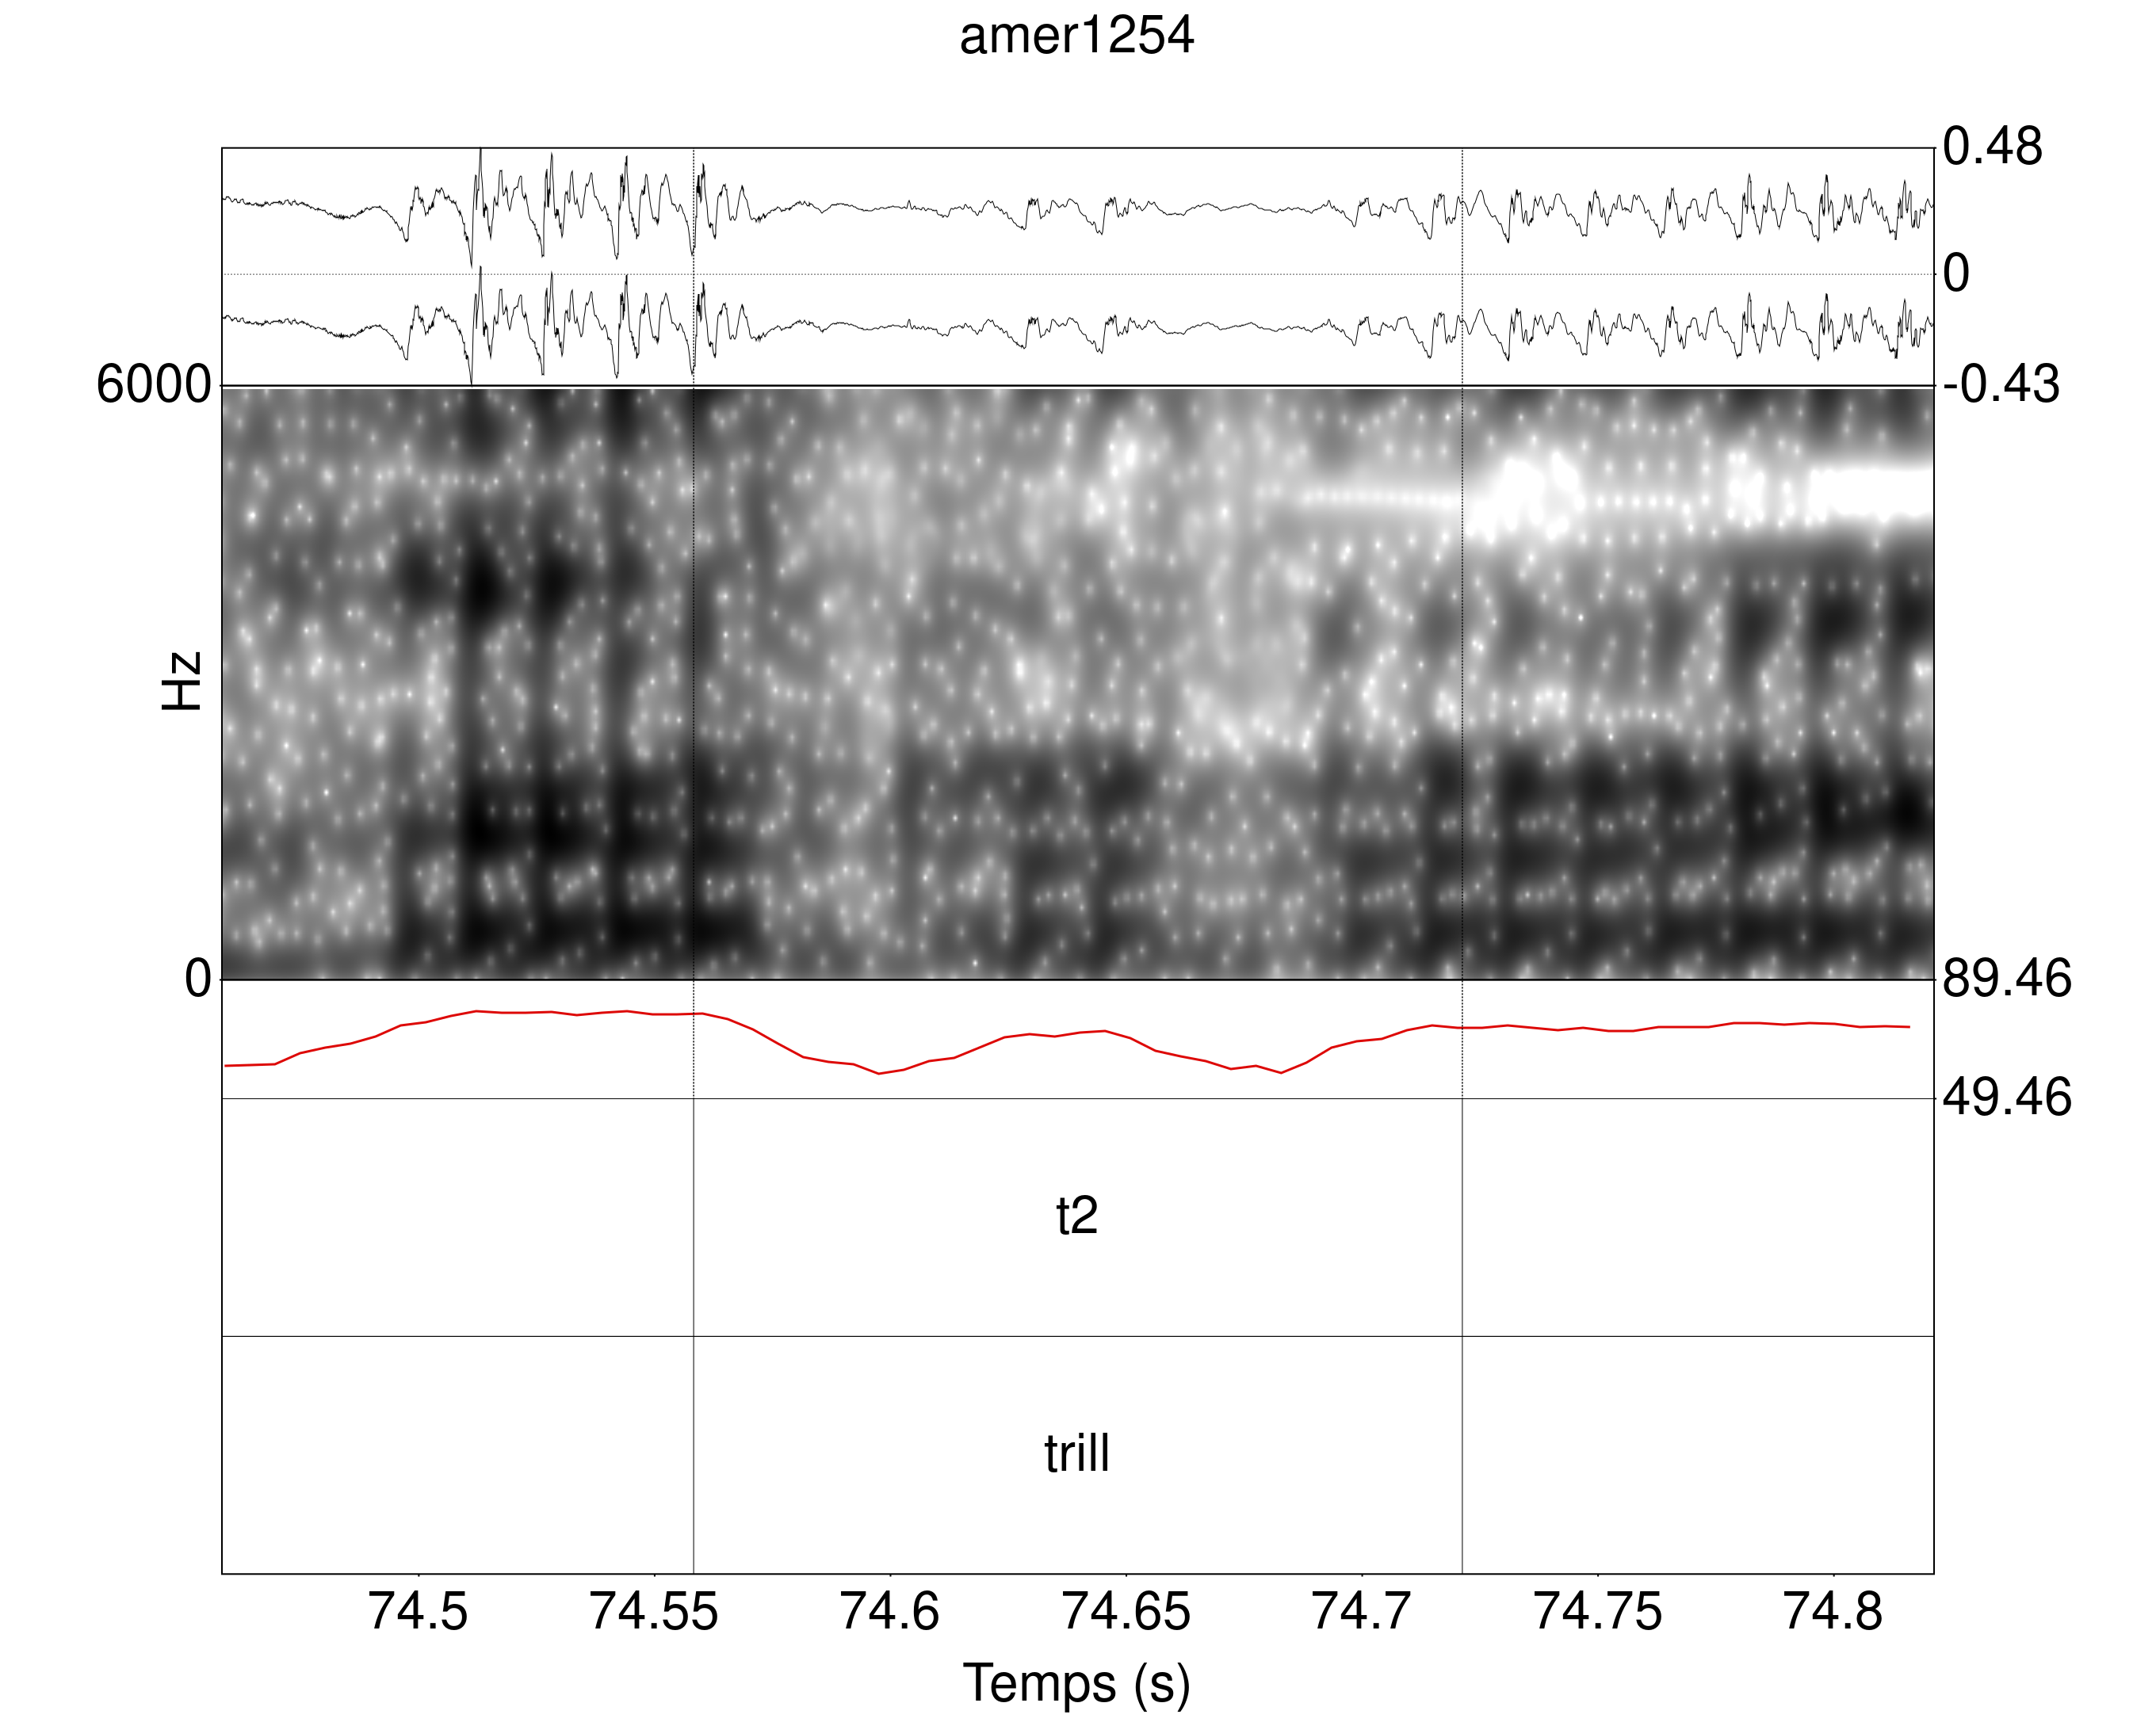
\includegraphics[width=0.45\linewidth]{substance/spectro_images/amer1254_67_62}
	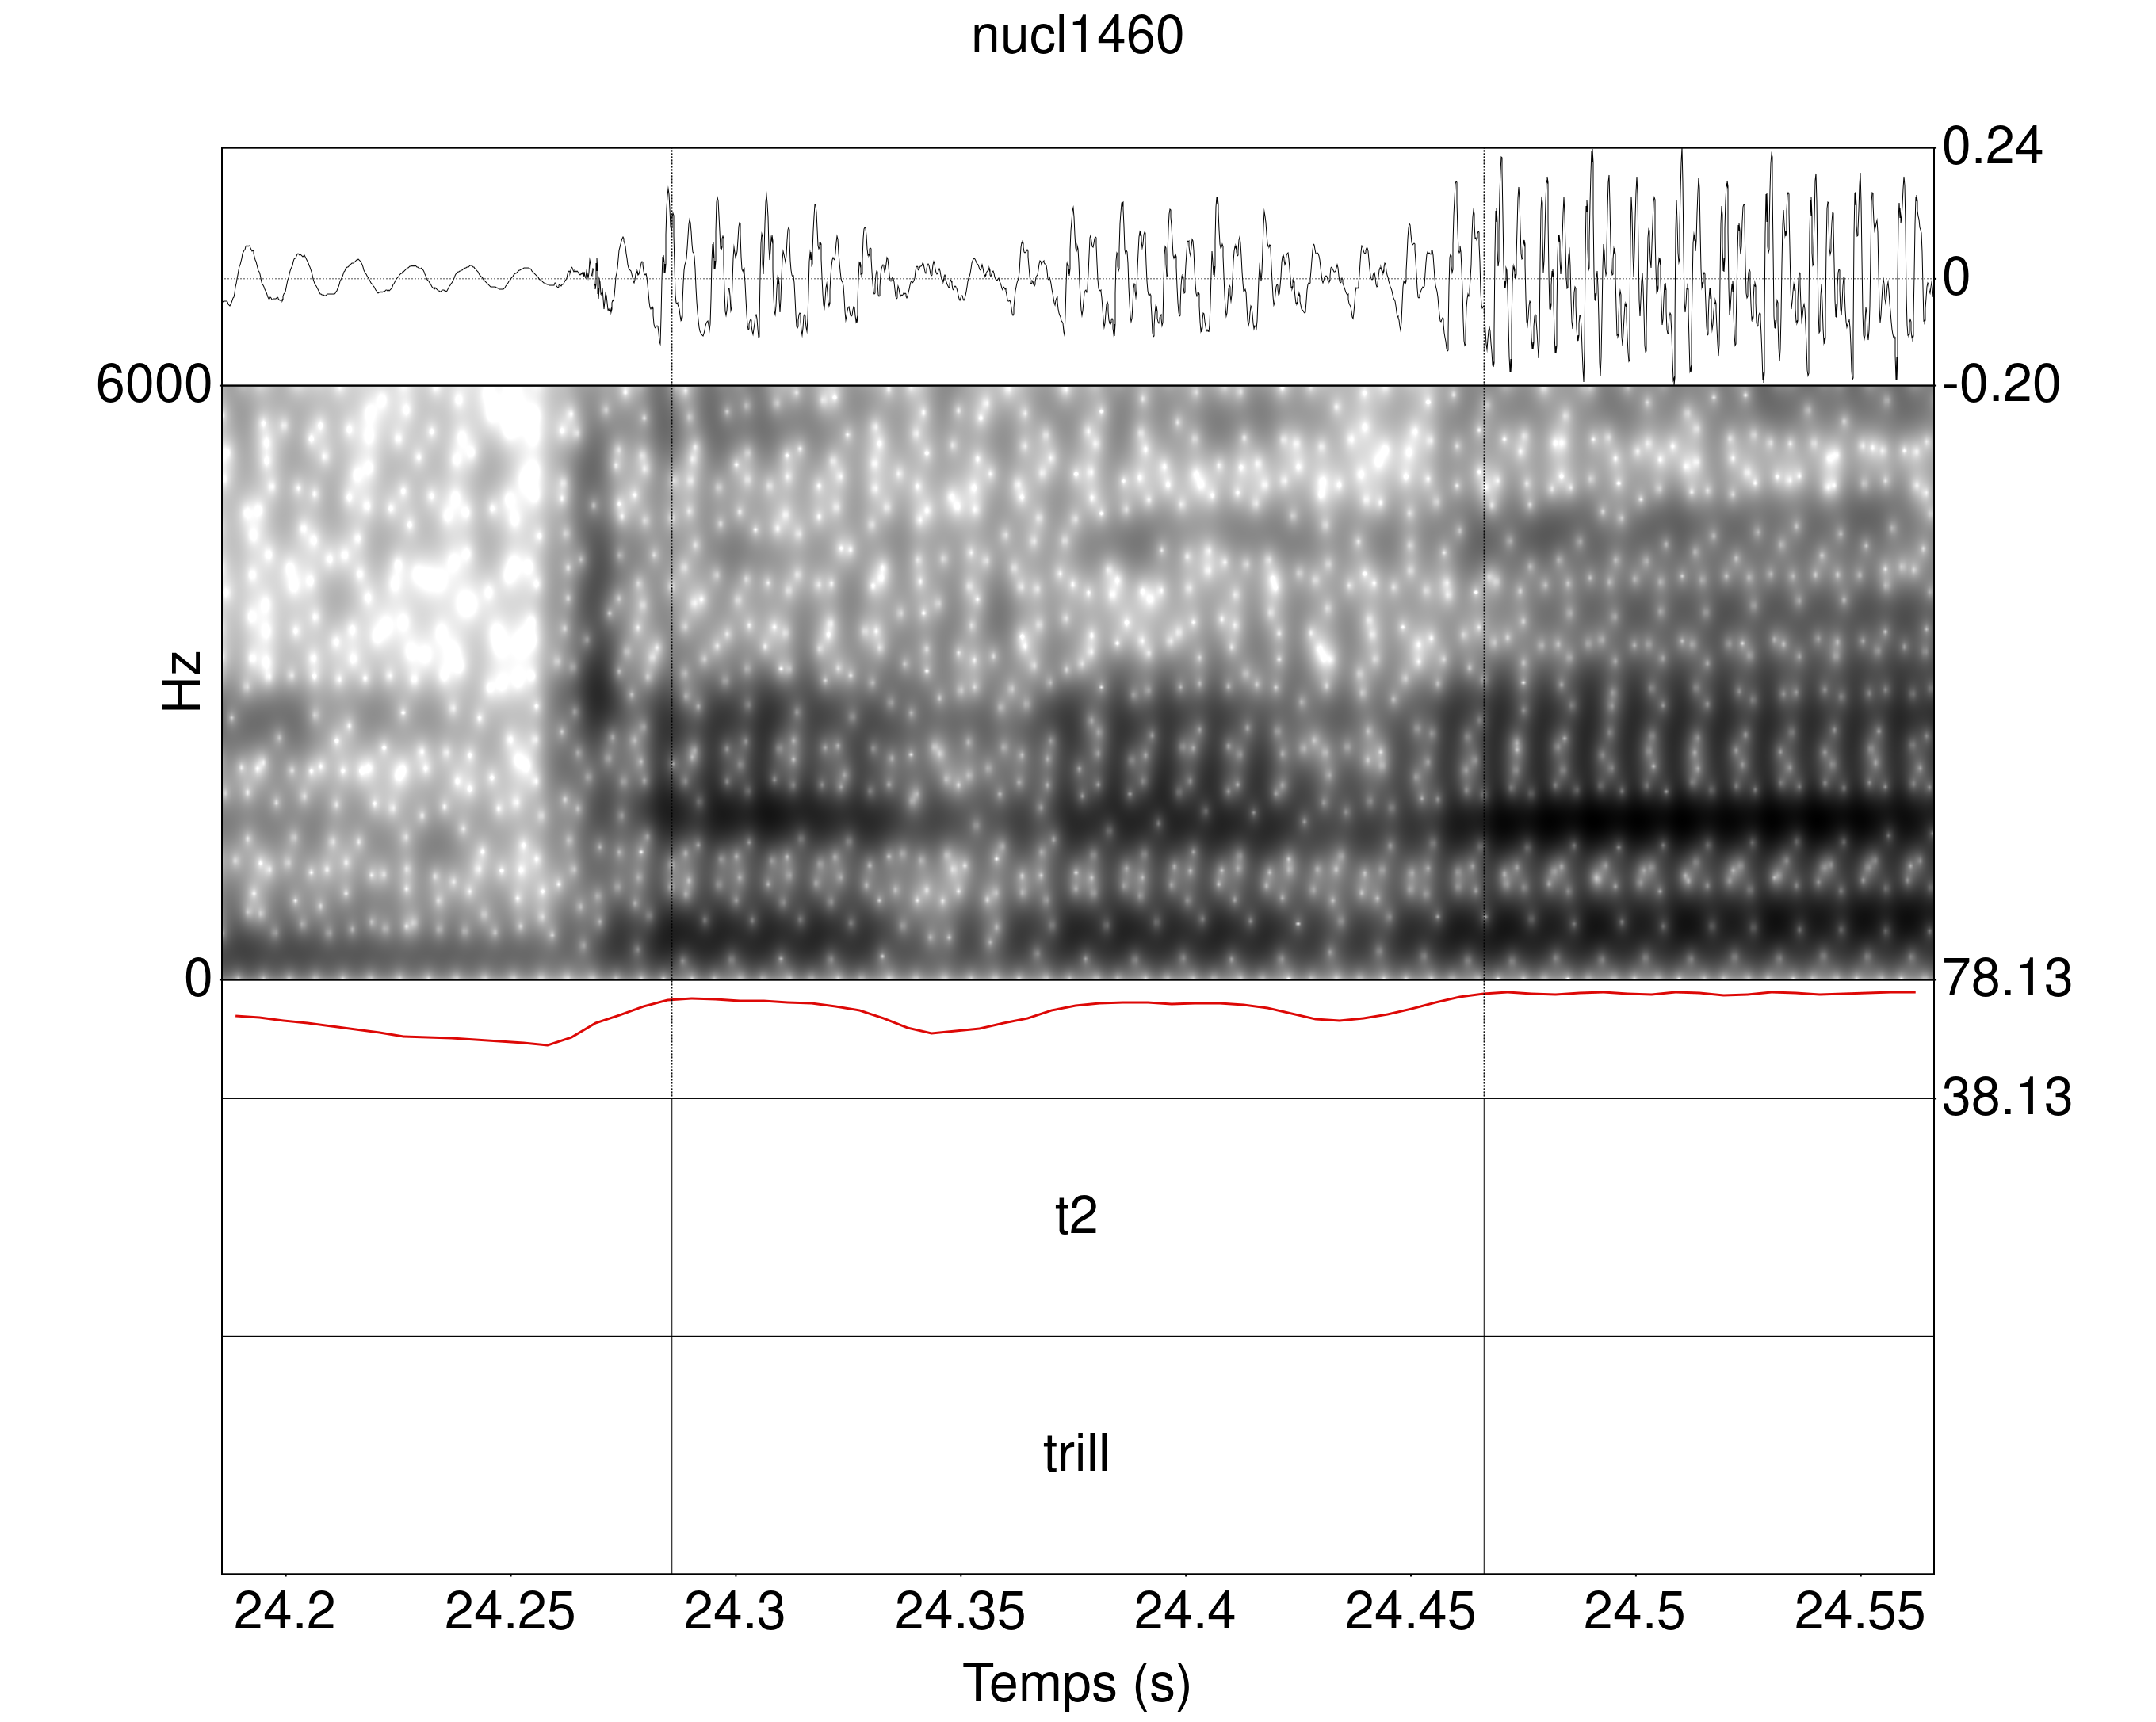
\includegraphics[width=0.45\linewidth]{substance/spectro_images/nucl1460_1338_16}
	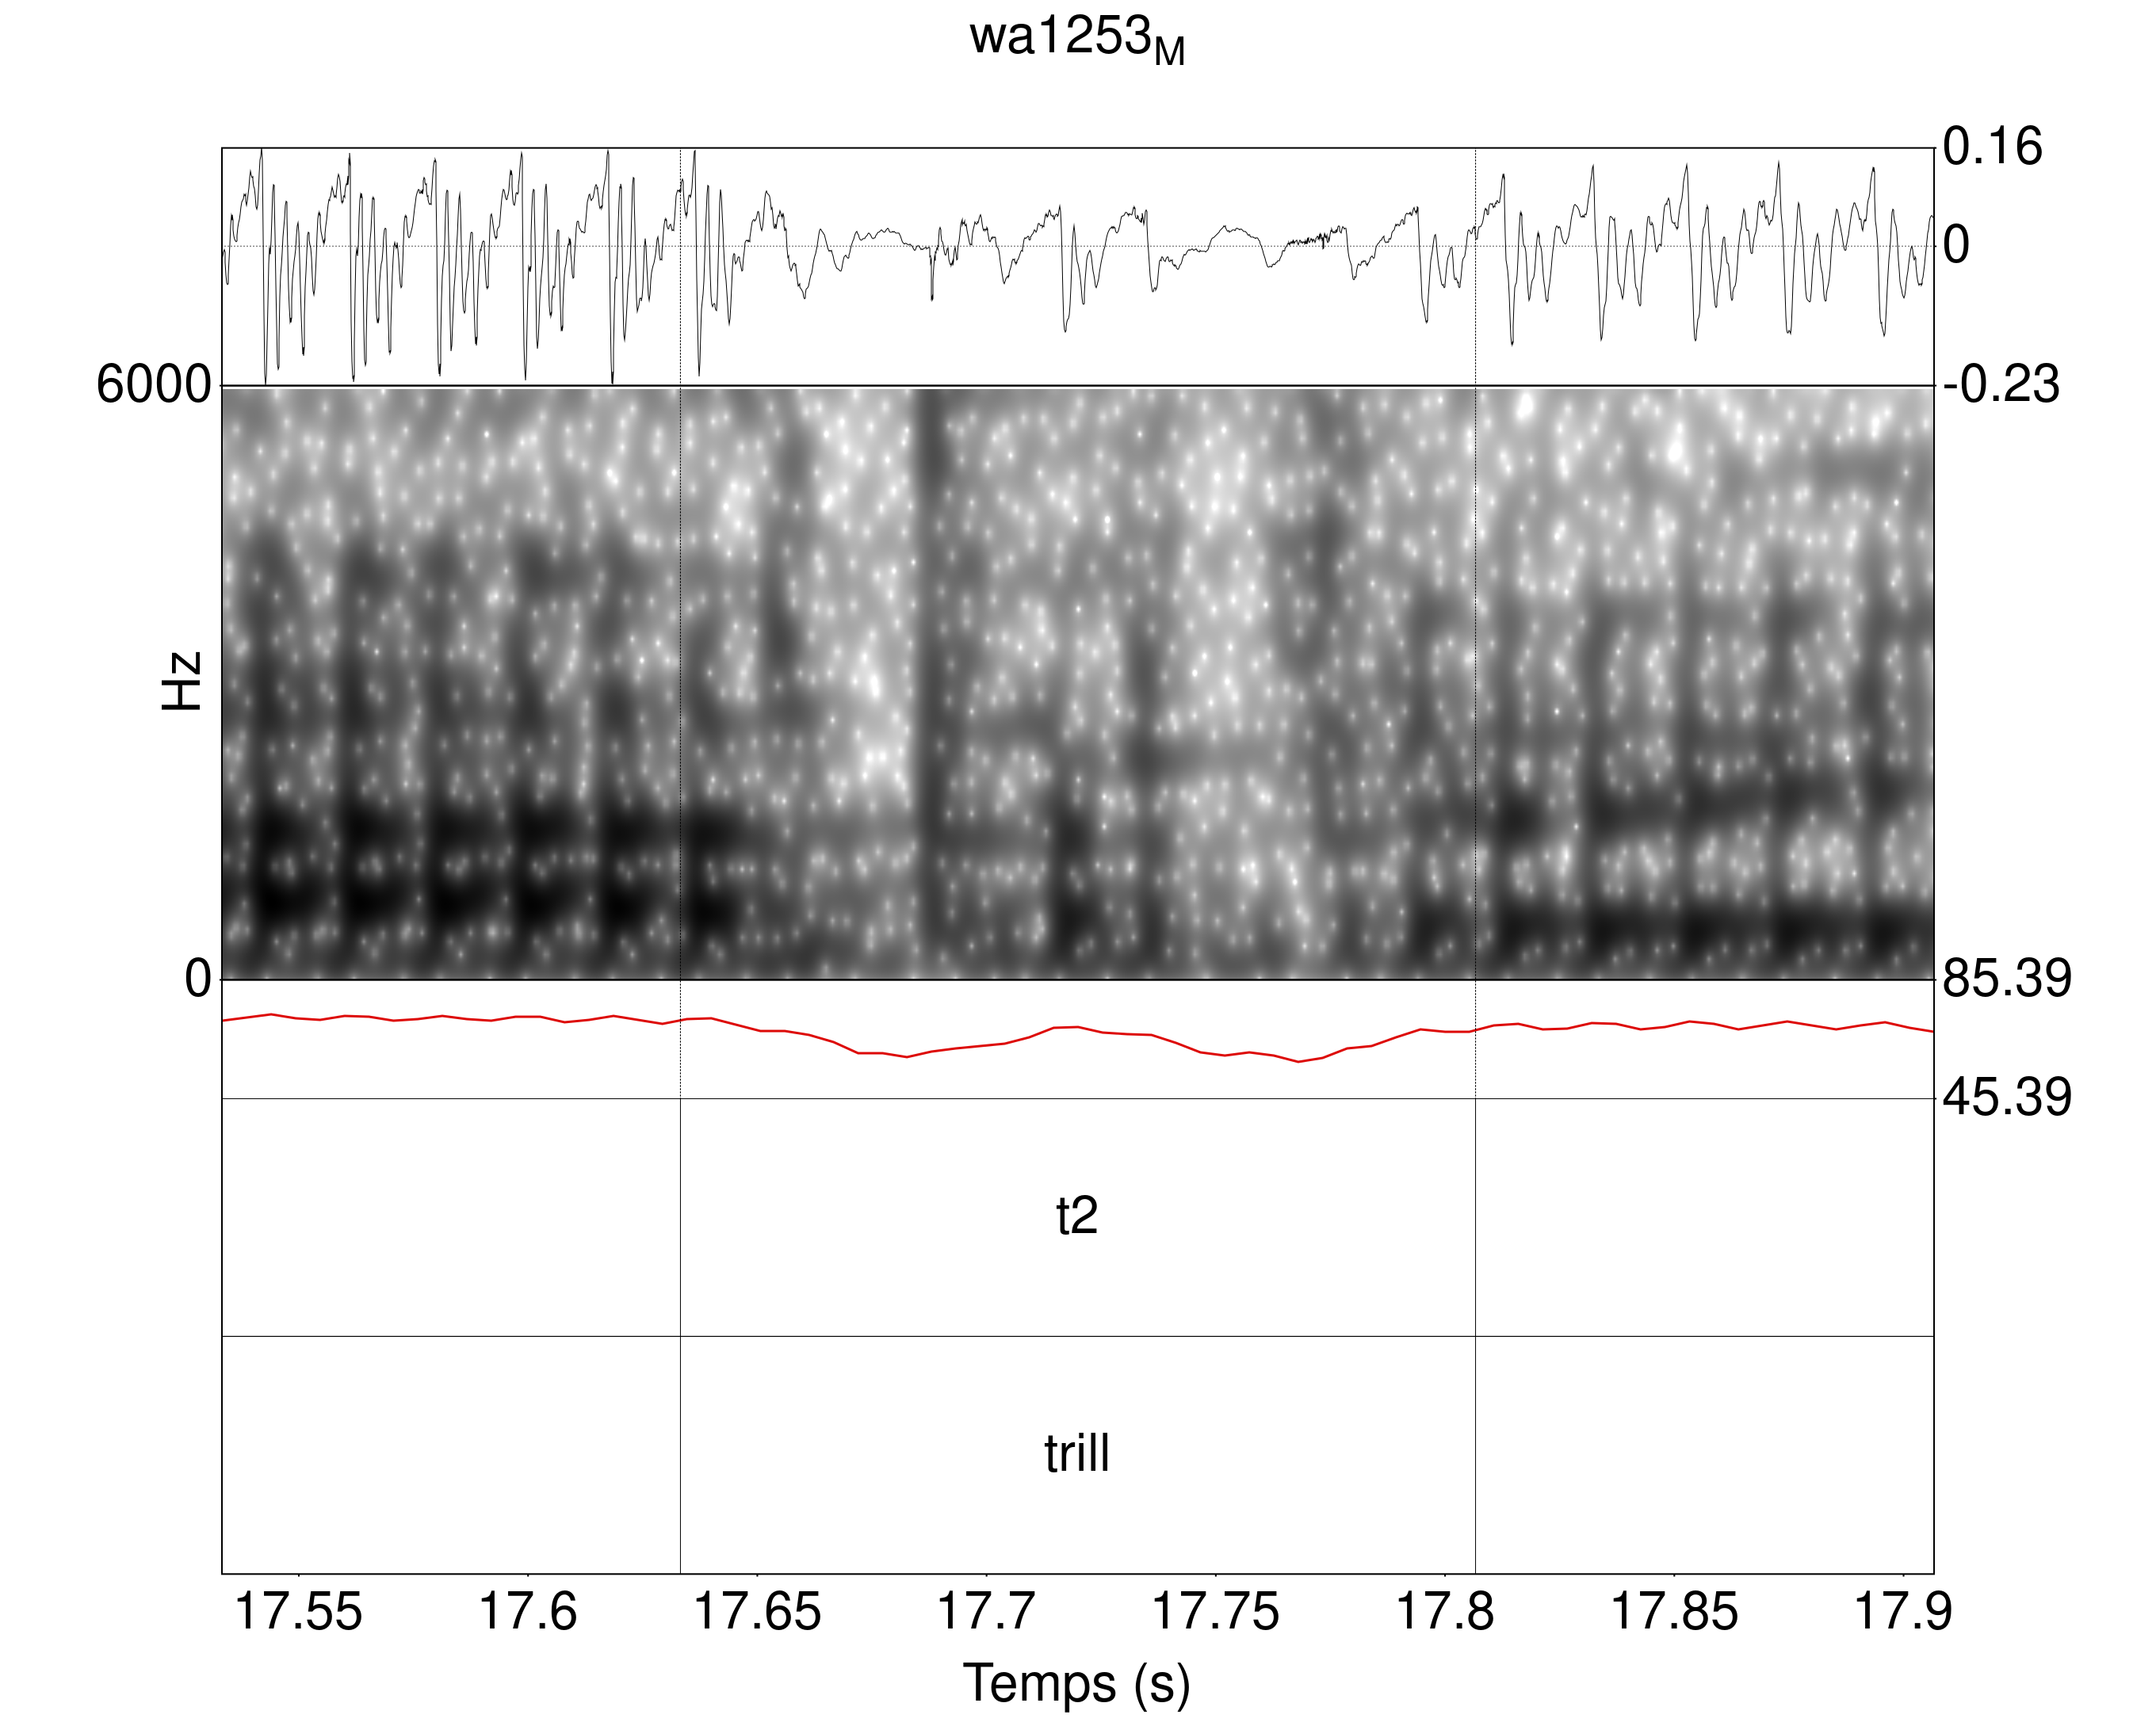
\includegraphics[width=0.45\linewidth]{substance/spectro_images/tswa1253_1703_6}
	\caption[Illustrations des \textg{t2} issus de 6 locuteurs et locutrices]{Illustrations avec oscillogrammes et spectrogrammes des \textg{t2} issus de locuteurs et locutrices
			du galicien \glotto{gali1258} (1 occurrence sur 1 de t2 soit 100\% des trills),
		    de l'espagnol castillan \glotto{cast1244} (2 occurrences sur 2 de t2 soit 100\% des trills),
		     du tamambo \glotto{malo1243} (15 occurrences sur 19 de t2 soit 78,9\% des trills),
		     de l'espagnol argentin \glotto{amer1254} (2 occurrences sur 3 de t2 soit 66,7\% des trills),
		     du madurais \glotto{nucl1460} (6 occurrences sur 8 de t2 soit 75\% des trills),
		     et du tswana \glotto{tswa1253} (3 occurrences sur 7 de t2 soit 42,9\% des trills).}
	\label{fig:galicastmalotswa}
\end{figure}

Dans un deuxième temps, nous nous intéressons aux segments labellisés comme taps, flaps et taps/flaps.
Sur les 27 locuteurs/trices qui produisent ces segments (\autoref{fig:variationtapflap}), cinq ont produit au moins un \textg{t2} (voir \autoref{fig:pashsanm} pour les illustrations acoustiques de deux segments issus de ces cinq locuteurs/trices).

\begin{figure}
	\centering
	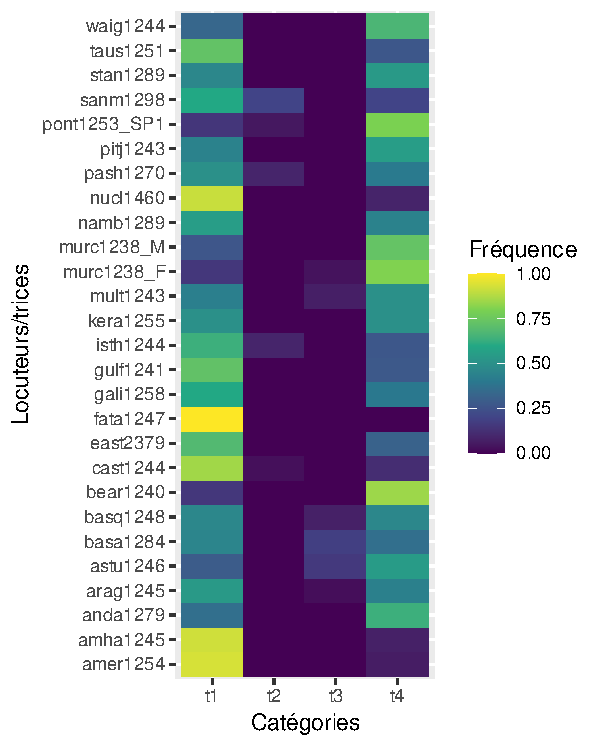
\includegraphics[width=0.45\linewidth]{substance/images/variation_tapflap}
	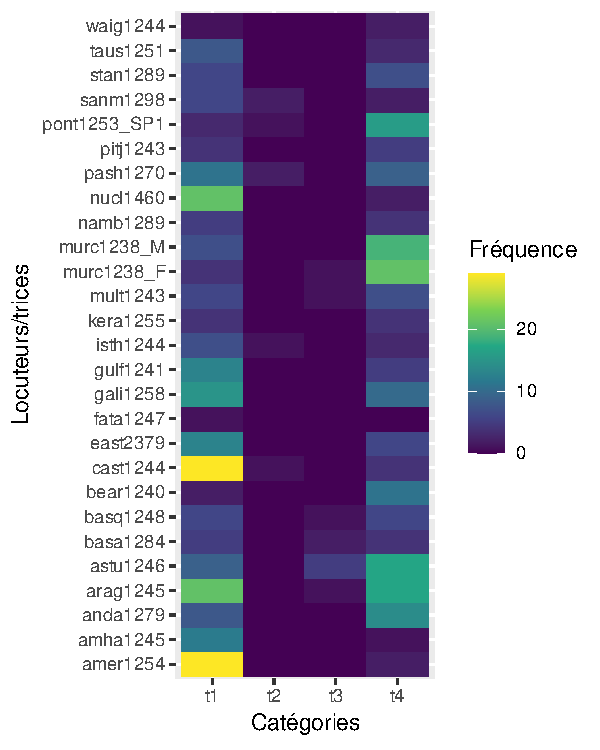
\includegraphics[width=0.45\linewidth]{substance/images/variation_tapflap_abs}
	\caption[Fréquences des différentes catégories illustrant la variation pour les segments ayant été catégorisés comme des \textg{taps, flaps et taps/flaps}]{Fréquences relatives (à gauche) et absolues (à droite) des différentes catégories illustrant la variation pour les segments ayant été catégorisés par les auteurs des illustrations comme des \textg{taps, flaps et taps/flaps}. Les fréquences sont calculées par ligne. Une case jaune est associée à une haute fréquence, cela veut dire que le/la locuteur/trice tend à produire une seule catégorie. Une case violette est associée à une catégorie non produite par le/la locuteur/trice.}
	\label{fig:variationtapflap}
\end{figure}

\begin{figure}
	\centering
	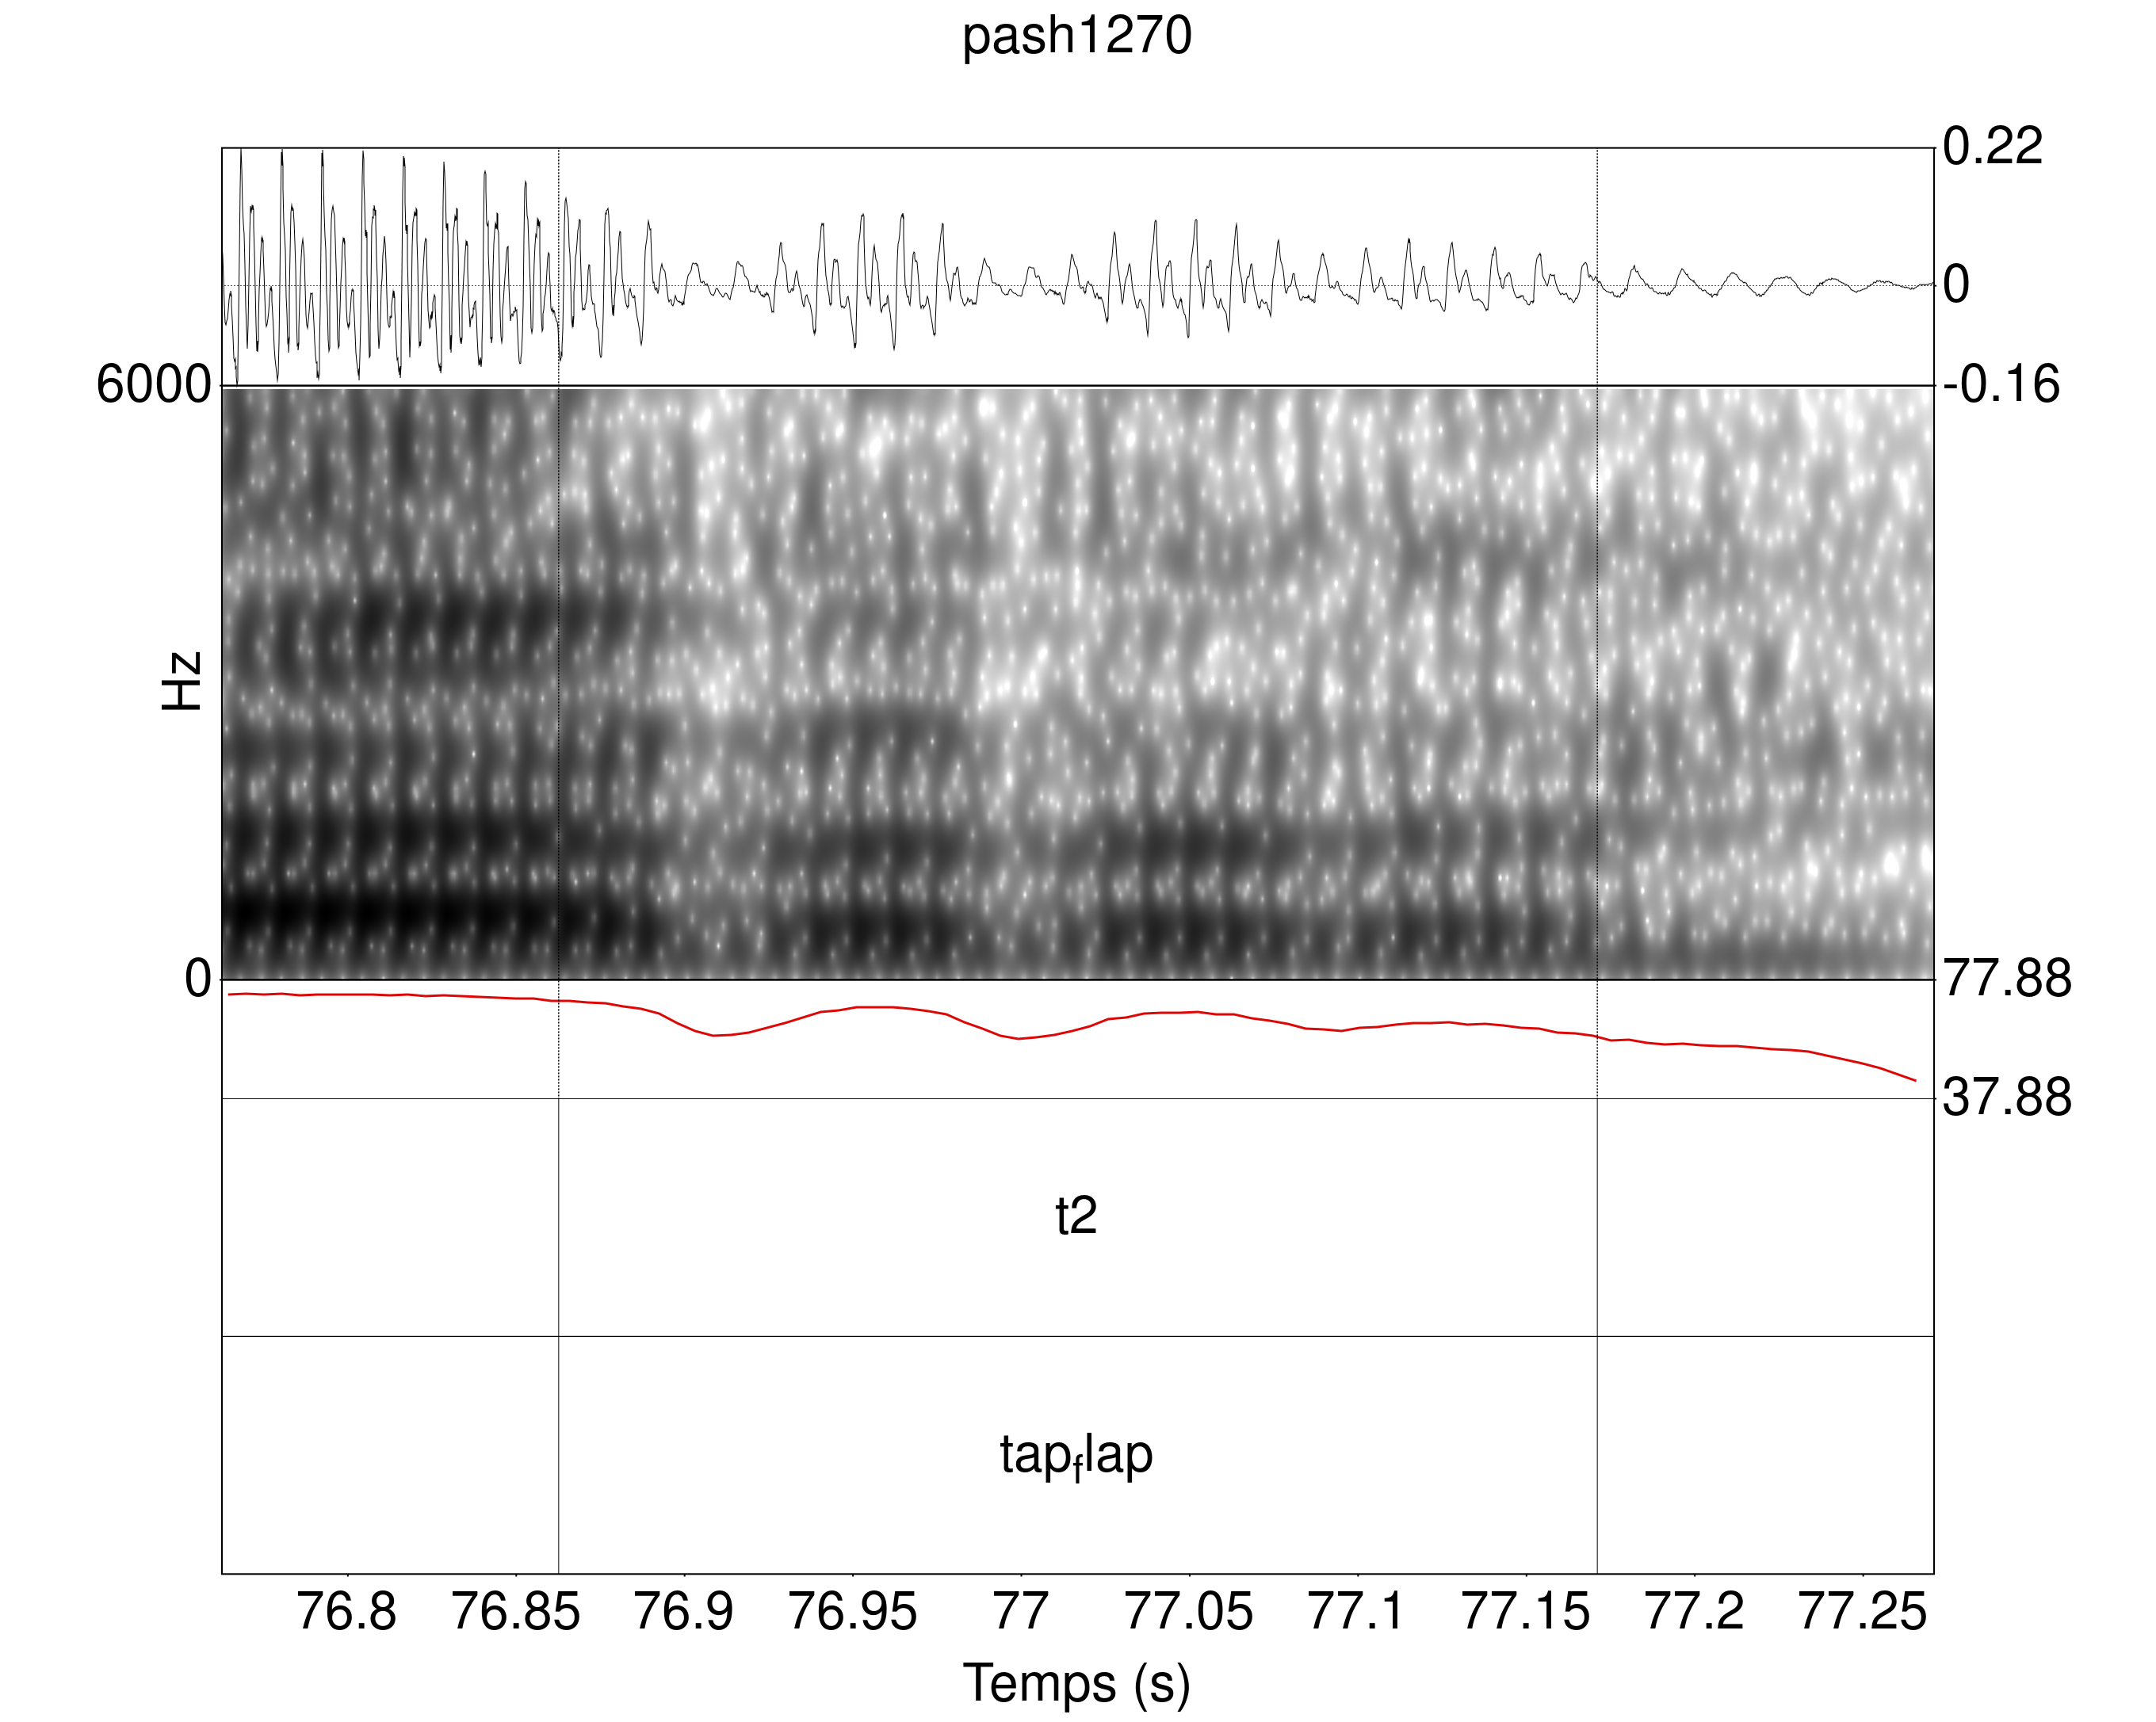
\includegraphics[width=0.45\linewidth]{substance/spectro_images/pash1270_1400_28}
	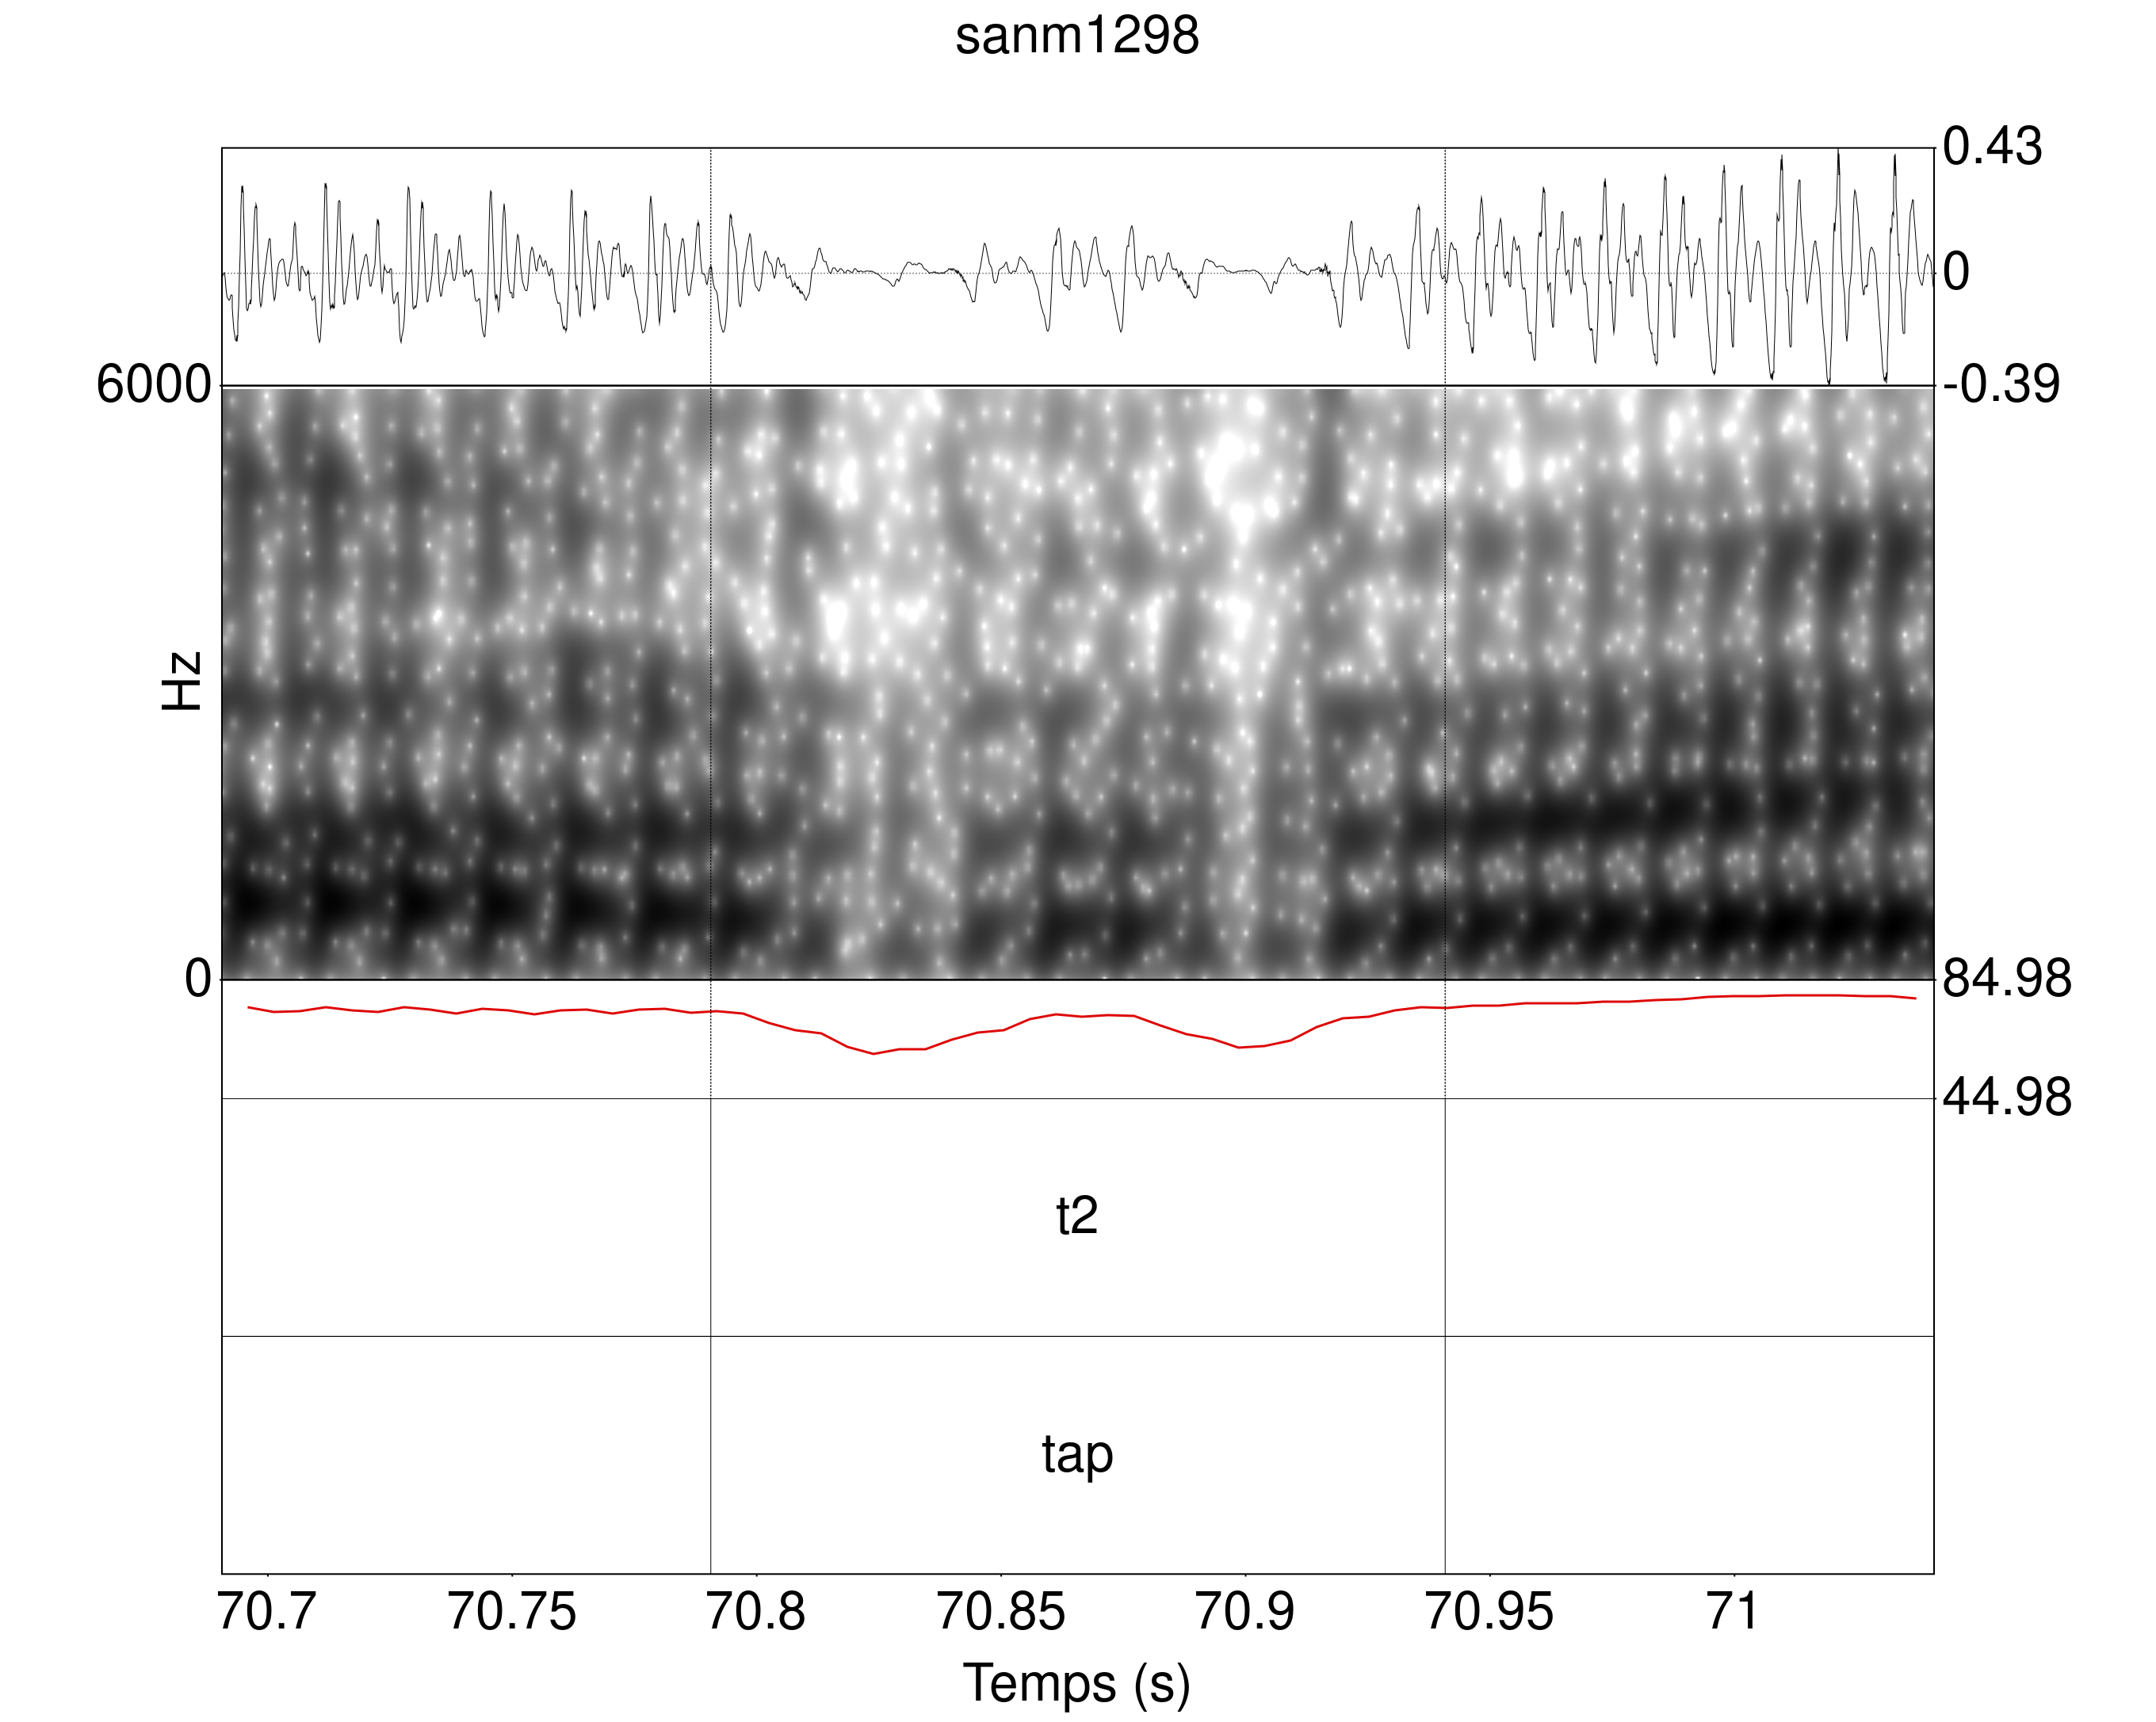
\includegraphics[width=0.45\linewidth]{substance/spectro_images/sanm1298_1558_6}
	\caption[Illustrations des \textg{t2} issus de 2 locuteurs/trices]{Illustrations des \textg{t2} issus de locuteurs/trices
		du pashai du sud est \glotto{pash1270} (2 occurrences sur 22 de t2 soit 9,1\% des trills) et 
		du galicien \glotto{gali1258} (2 occurrences sur 10 de t2 soit 100\% des trills). De haut en bas pour chacune des illustrations, nous avons l'oscillogramme, le spectrogramme, la courbe d'intensité, un palier intervallique avec la catégorie segmentée, et un palier intervallique comprenant le label descriptif du segment d'intérêt.}
	\label{fig:pashsanm}
\end{figure}


Finalement, nous nous intéressons aux segments labellisés comme \textg{trills/taps} et \textg{trills/flaps} avec quatre locuteurs/trices (\autoref{fig:variationtrillother}) dont deux produisent au moins un \textg{t2} comme illustré dans la \autoref{fig:platindo}.

\begin{figure}
	\centering
	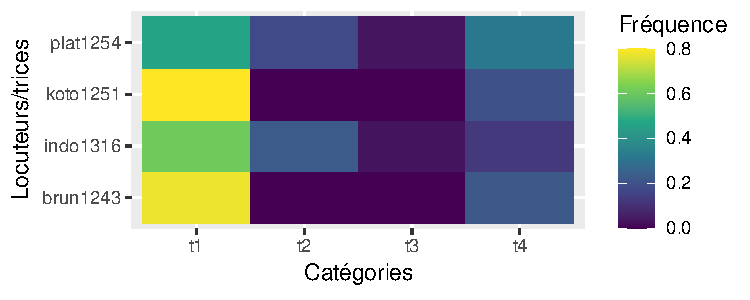
\includegraphics[width=0.45\linewidth]{substance/images/variation_trillother}
	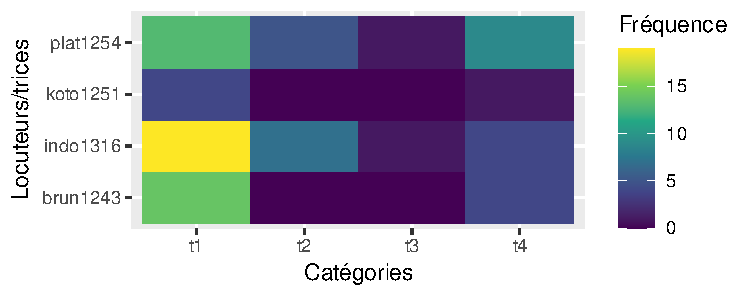
\includegraphics[width=0.45\linewidth]{substance/images/variation_trillother_abs}
	\caption[Fréquences relatives des différentes catégories illustrant la variation pour les segments ayant été catégorisés comme des \textg{trills/taps et trills/flaps}]{Fréquences relatives (à gauche) et absolues (à droite) des différentes catégories illustrant la variation pour les segments ayant été catégorisés par les auteurs des illustrations comme des \textg{trills/taps et trills/flaps}. Les fréquences sont calculées par ligne. Une case jaune est associée à une haute fréquence, cela veut dire que le/la locuteur/trice tend à produire une seule catégorie. Une case violette est associée à une catégorie non produite par le/la locuteur/trice.}
	\label{fig:variationtrillother}
\end{figure}


\begin{figure}
	\centering
	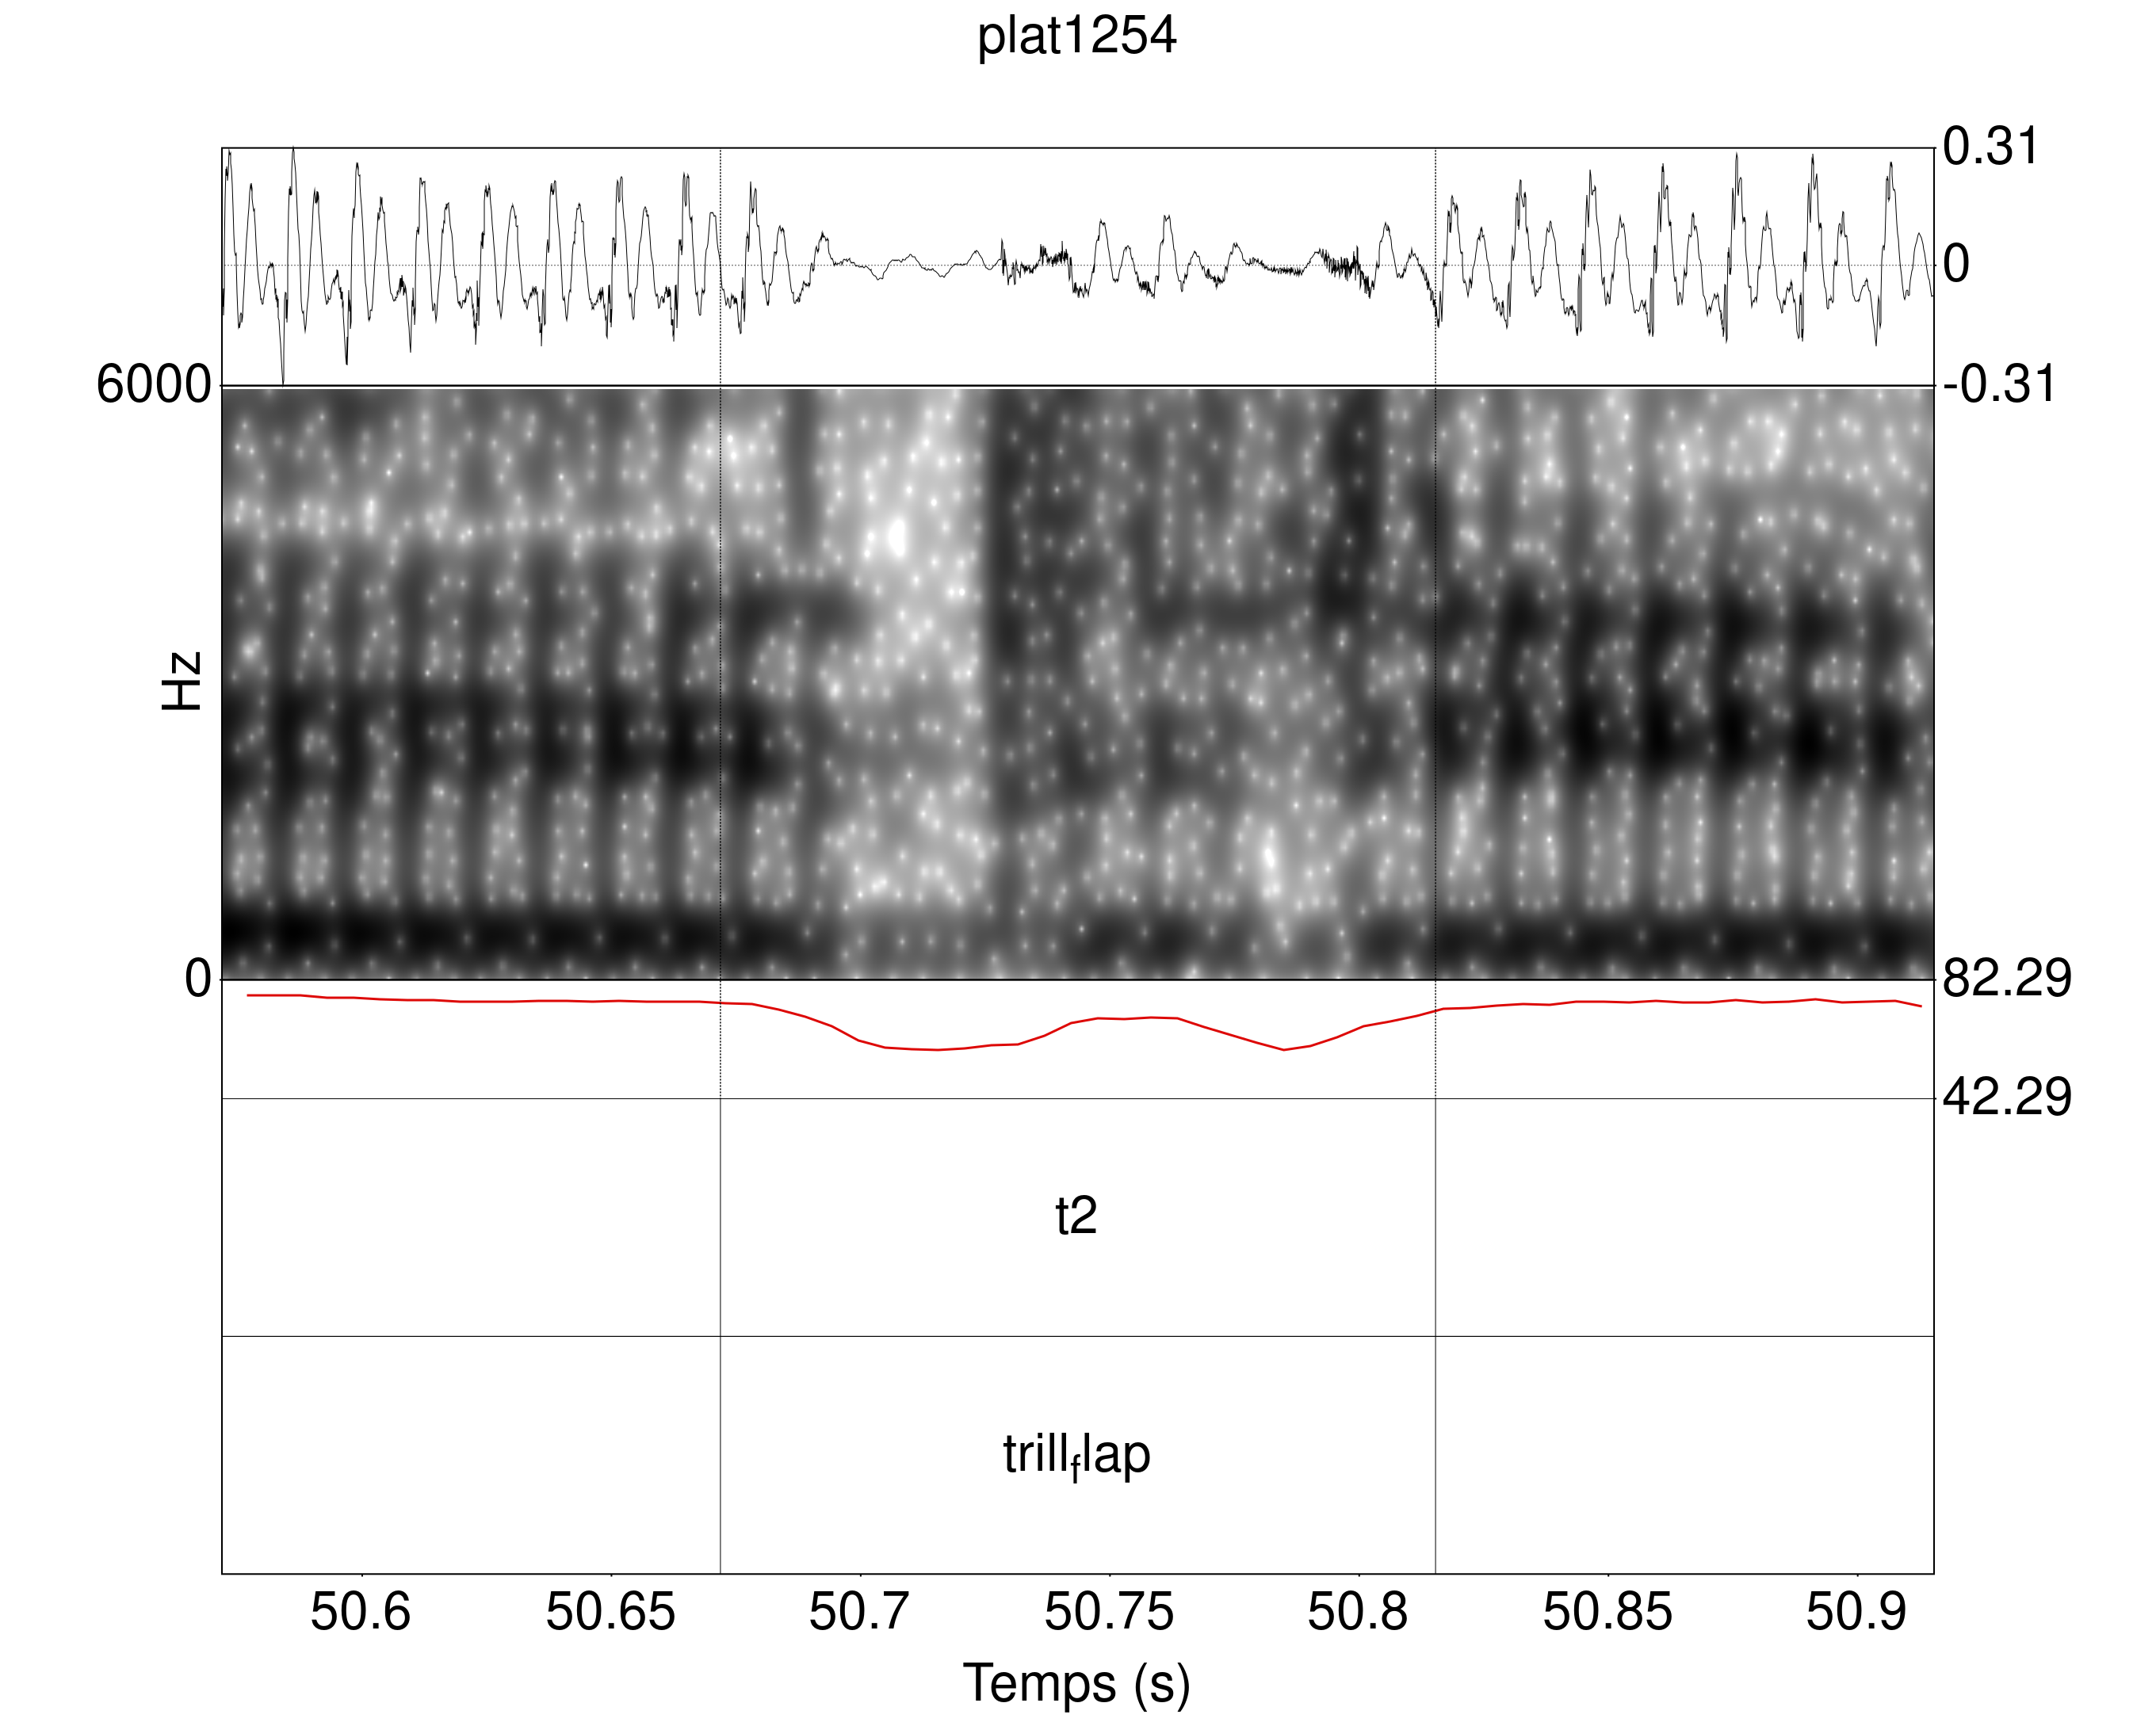
\includegraphics[width=0.45\linewidth]{substance/spectro_images/plat1254_1457_34}
	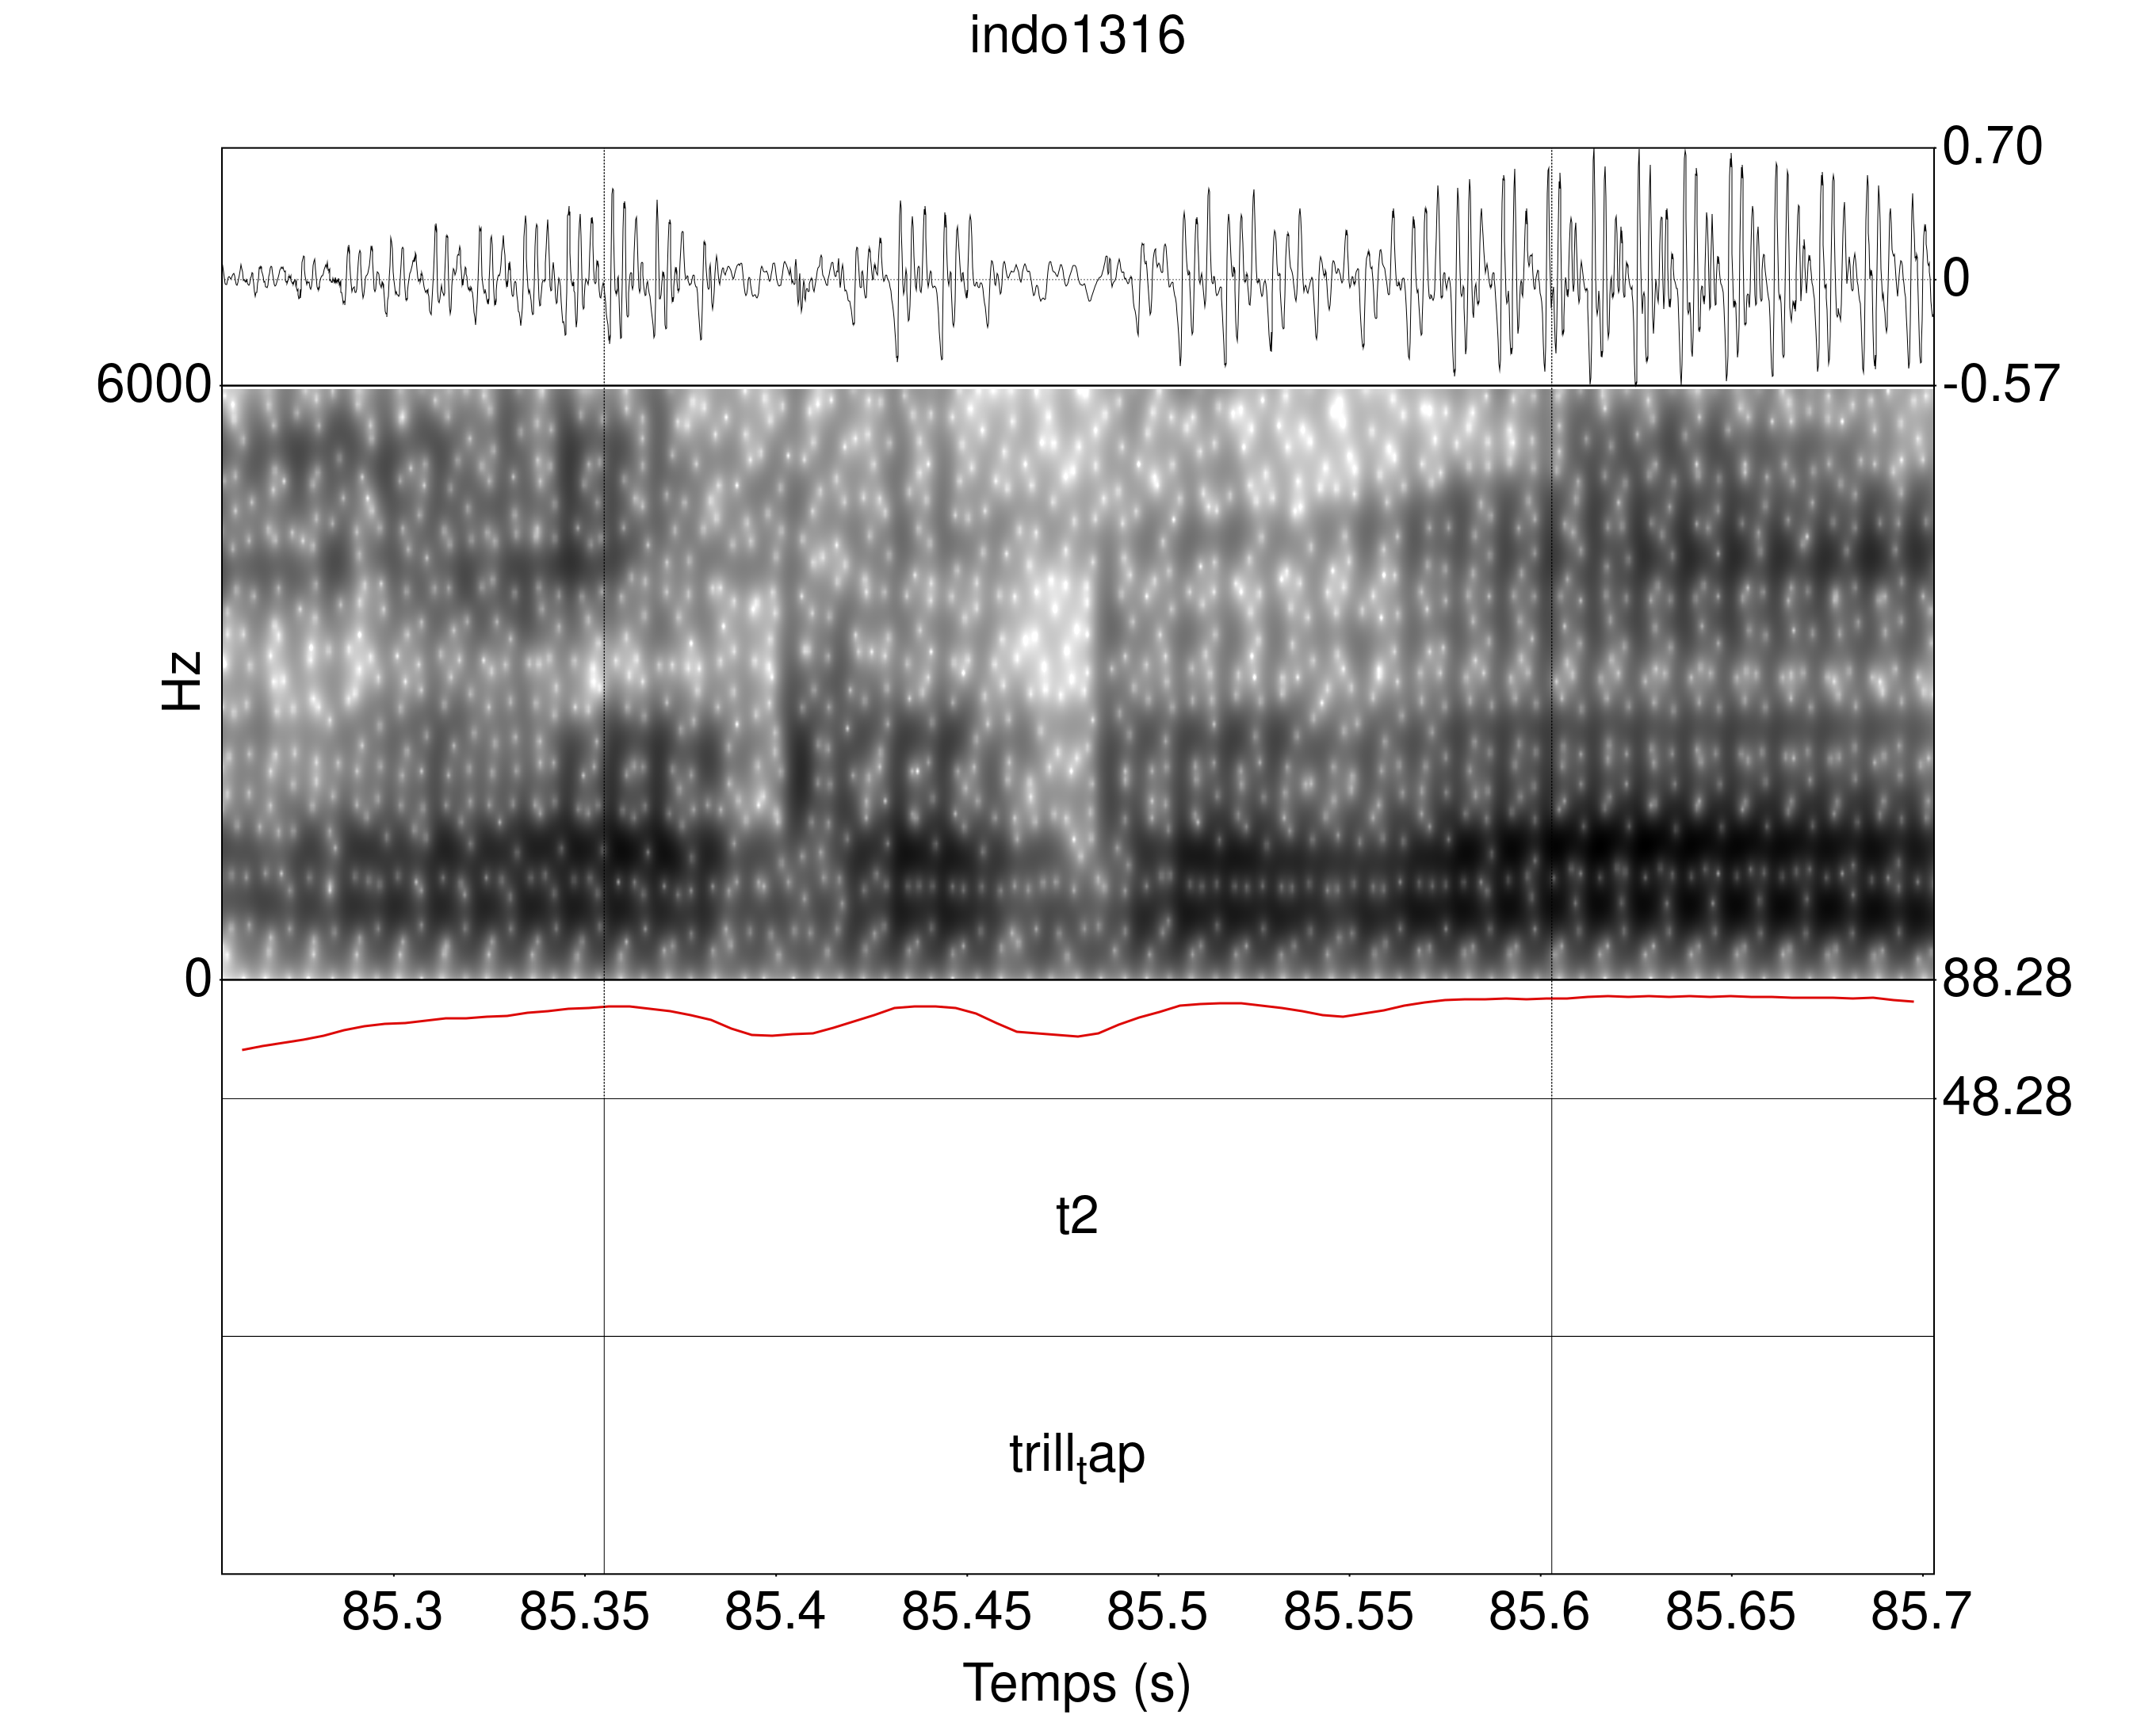
\includegraphics[width=0.45\linewidth]{substance/spectro_images/indo1316_858_34}
	\caption[Illustrations des \textg{t2} issus de locuteurs/trices]{Illustrations des \textg{t2} issus de locuteurs/trices
		de l'indonésien \glotto{indo1316} (7 occurrences sur 31 de t2 soit 22,6\% des trills) et 
		du malgache central \glotto{plat1254} (5 occurrences sur 28 de t2 soit 17,9\% des trills). De haut en bas pour chacune des illustrations, nous avons l'oscillogramme, le spectrogramme, la courbe d'intensité, un palier intervallique avec la catégorie segmentée, et un palier intervallique comprenant le label descriptif du segment d'intérêt.}
	\label{fig:platindo}
\end{figure}


\section{Deuxième étude : étude des composants des trills et taps}

La deuxième étude fait appel à une méthodologie plus précise que la première. Cette étude fait particulièrement attention à la segmentation. Du fait du peu de données, cette étude présente aussi des schémas idiosyncratiques. Les productions des rhotiques entre et au sein des individus varient.\\

Pour l'annotation, nous avons choisi de prendre en compte quatre unités de base pour la segmentation, que nous appellerons les \textg{éléments}.
Dans cette partie, nous illustrons les différents éléments ainsi que les motifs (les combinaisons d'éléments) avec des spectrogrammes. Nous considérons ces spectrogrammes comme \textg{prototypiques}, cependant, il faut prendre en compte que nous avons fait face à beaucoup de variation pendant le processus de segmentation et d'annotation. La mise en place des frontières sur le signal n'est pas toujours évidente. De plus, l'étape de segmentation a été mise en difficulté par la qualité des audios qui diffère d'une langue à une autre. Ainsi, dans certains cas, il a fallu s'appuyer plus sur la perception du son que sur la visualisation du signal acoustique\footnote{C'est le cas principalement des audios du mavea \glotto{mafe1237}.} (les TextGrids des différentes annotations sont mises à disposition sur \href{https://github.com/ranselme}{github.com/ranselme}).

Dans un premier temps, nous nous intéressons à la description des différents éléments, puis nous analysons la diversité des motifs obtenus. Nous nous concentrons sur la durée des motifs ainsi que sur les contextes des motifs les plus fréquents.

\subsection{Le \textg{o} : élément d'occlusion}

\begin{figure}
	\centering
	\includegraphics[width=0.8\linewidth]{substance/spectro_images/east2379_584_ɛrə}
	\caption[Illustration de l'élément \textg{o}]{Illustration de l'élément \textg{o} dans le contexte [ɛɾə] en arrernte central. De haut en bas, nous avons l'oscillogramme, le spectrogramme, la courbe d'intensité, un palier intervallique avec la catégorie segmentée, et un palier intervallique comprenant le label descriptif du segment d'intérêt.}
	\label{fig:east2379584r}
\end{figure}


Le premier élément que nous choisissons de décrire est l'élément \textg{o}. \textcite[65]{blecuaVibrantesEspanolManifestaciones2002} parle d'un élément correspondant à une phase brève de silence avec une barre de voisement. Cet élément peut se rencontrer indépendamment et former un segment à lui seul, ou peut se combiner avec d'autres éléments. \\

Sur le spectrogramme cet élément est reconnaissable par une baisse de l'énergie se traduisant par une zone plus \textg{blanche} (\autoref{fig:east2379584r}). De plus, on retrouve une baisse de l'intensité ainsi qu'une baisse de l'amplitude. Le signal n'est généralement pas périodique. Nous avons fait le choix de ne pas nous intéresser au voisement, ainsi nous ne faisons pas de distinction entre les \textg{o} voisés et les \textg{o} non-voisés.\\

La durée moyenne, tous contextes confondus, de l'élément \textg{o} est de 21,30 ms, sa médiane de 20,88 ms (minimum de 8,60 ms, maximum de 42,31 ms, IQR [écart interquartile] de 7,38 ms).


\subsection{Le \textg{b} : élément de relâchement (burst)}

\begin{figure}
	\centering
	\includegraphics[width=0.8\linewidth]{substance/spectro_images/indo1317_477_}
	\caption[Illustration de l'élément \textg{b}]{Illustration de l'élément \textg{b} dans le contexte [ɯɾi] en indonésien des Bajau (Lombok de l'est). De haut en bas, nous avons l'oscillogramme, le spectrogramme, la courbe d'intensité, un palier intervallique avec la catégorie segmentée, et un palier intervallique comprenant le label descriptif du segment d'intérêt.}
	\label{fig:indo1317477}
\end{figure}

Le deuxième élément \textg{b} n'apparaît jamais en isolation et est systématiquement précédé d'un élément \textg{o} alors que le contraire n'est pas vrai. En effet, c'est la pression lors de l'occlusion qui entraîne cet élément \textg{b}. Il ne s'agit pas d'un élément vocalique mais d'un élément similaire à une occlusive avec une barre d'explosion (plus ou moins marquée) suivie d'un signal apériodique similaire (\autoref{fig:indo1317477}). \textcite[28]{skarnitzlPrinciplesPhoneticSegmentation2011} rappellent que les occlusives sont composées de plusieurs propriétés phonétiques inhérentes, parmi lesquelles on retrouve entre autres une fermeture complète au niveau du lieu d'articulation entraînant l'absence de structure formantique, et expliquant ainsi la présence d'un relâchement sous la forme de bruit d'explosion. \textcite[72]{skarnitzlPrinciplesPhoneticSegmentation2011} mentionnent que le cycle du [r] (à partir du spectrogramme qui accompagne sa description, on peut dire qu'ils illustrent leurs propos avec un motif \textg{ob}) peut être accompagné de \textg{plosion-like noise}.
Il n'y a donc pas de contre-indications à voir ce signal apériodique comme comparable au moment du relâchement dans une occlusive. On retrouve beaucoup d'énergie similaire à de la friction dans certains cas, avec parfois le début d'un signal périodique bruité.\\

\textcite[87]{blecuaVibrantesEspanolManifestaciones2002} mentionne cet élément dans sa section des taps en attaques complexes sans le catégoriser comme tel en parlant de certains éléments vocaliques : \textg{también se observan realizaciones en las que el elemento esvarabático es muy breve, e incluso podría llegar a confundirse con una barra de explosión}\footnote{Trad. : \textg{on observe aussi des réalisations dans lesquelles l'élément svarabhaktique est très bref, et qui pourrait être confondu avec une barre d'explosion}}. La mention de cet élément est aussi présente dans sa section sur les taps en codas (p. 152), sur les taps en position intervocalique (p. 198), ainsi que sur les trills en position intervocalique (cf. figure 96 page 238 reproduite en \autoref{fig:blecuafigure96}).\\

\begin{figure}
	\centering
	\includegraphics[width=0.8\linewidth]{substance/spectro_images/blecua_figure96}
	\caption[Illustration d'un élément \textg{o} par \textcite{blecuaVibrantesEspanolManifestaciones2002}]{Illustration d'un élément \textg{o} par \textcite[238]{blecuaVibrantesEspanolManifestaciones2002} où on retrouve aussi l'élément \textg{b}. [Trad : Spectrogramme et oscillogramme de la séquence \textit{a relaja(rte)}. Réalisation classifiée comme \textit{occlusion}].}
	\label{fig:blecuafigure96}
\end{figure}

La durée moyenne, tous contextes confondus, de l'élément \textg{b} est de 14,46 ms, sa médiane de 12,54 ms (minimum de 4,85 ms, maximum de 55,33 ms, IQR [écart interquartile] de 6,81 ms).\\



\subsection[Le \textg{a} : élément de constriction sans occlusion complète]{Le \textg{a} : élément de constriction sans occlusion complète (approximante)}

L'élément \textg{a} est un élément qui a été caractérisé par \textg{cualquier realización en la que se observe estructura formántica}\footnote{Trad. : \textg{n'importe quelle réalisation dans laquelle on observe une structure formantique}} \textcite[68]{blecuaVibrantesEspanolManifestaciones2002}. Pour qu'un élément appartienne à cette catégorie, il doit avoir une structure formantique au niveau du spectrogramme et un signal relativement similaire à un signal périodique (\autoref{fig:sout26041312r}). Nous avons aussi pris en compte une diminution de l'intensité nécessaire (même légère) pour que l'élément puisse être classé dans cette catégorie.

\begin{figure}
	\centering
	\includegraphics[width=0.7\linewidth]{substance/spectro_images/sout2604_1312_ɛrɛ}
	\caption[Illustration de l'élément \textg{a}]{Illustration de l'élément \textg{a} dans le contexte [ɛrɛ] en ukrainien. De haut en bas, nous avons l'oscillogramme, le spectrogramme, la courbe d'intensité, un palier intervallique avec la catégorie segmentée, et un palier intervallique comprenant le label descriptif du segment d'intérêt.}
	\label{fig:sout26041312r}
\end{figure}

La durée moyenne, tous contextes confondus, de l'élément \textg{a} est de 31,34 ms, sa médiane de 25,56 ms (minimum de 10,71 ms, maximum de 123,71 ms, IQR [écart interquartile] de 14,61 ms).


\subsection[Le \textg{c} : élément épenthétique vocalique]{Le \textg{c} : élément épenthétique vocalique\\ (élément \textg{svarabhaktique})}


Enfin, le dernier élément que nous avons décidé d'annoter est le \textg{c}. \textcite[38]{blecuaVibrantesEspanolManifestaciones2002} mentionne qu'il s'agit d'un élément avec des caractéristiques similaires à celles d'une voyelle courte, et qui possède donc des formants, bien que son intensité soit inférieure à celle de la voyelle suivante. Elle rapporte en citant Quilis (1970)\footnote{Quilis, A.(1970): \textg{El elemento esvarabático en los grupos [pr, br, tr...]}, dans \textit{Phonétique et linguistique romanes : Mélanges offerts à M.Georges Straka}, Lyon-Strasbourg, Societé de Linguistique Romane, I. pp. 99-104.} que sa durée est comprise entre 8 et 56 ms avec une durée moyenne de 32 ms.\\

\begin{figure}
	\centering
	\includegraphics[width=0.8\linewidth]{substance/spectro_images/gayo1244_446_}
	\caption[Illustration de l'élément \textg{c}]{Illustration de l'élément \textg{c} dans le contexte [ˈkras] en gayo. De haut en bas, nous avons l'oscillogramme, le spectrogramme, la courbe d'intensité, un palier intervallique avec la catégorie segmentée, et un palier intervallique comprenant le label descriptif du segment d'intérêt.}
	\label{fig:gayo1244446}
\end{figure}

Il était parfois difficile de faire la différence entre un élément \textg{a} et un élément \textg{c}.
Par conséquent, nous avons essayé de nous référer à l'intensité qui a tendance à augmenter pour les éléments \textg{c} contrairement aux \textg{a} où elle diminue. Nous notons que certains cas restent problématiques à cause de structures non périodiques que nous avons tout de même choisi d'annoter comme \textg{c} (\autoref{fig:gayo1244446}).

La durée moyenne, tous contextes confondus, de l'élément \textg{c} est de 21,40 ms, sa médiane de 19,31 ms (minimum de 10,71 ms, maximum de 59,69 ms, IQR [écart interquartile] de 10,04 ms).

\section{Présentation des 18 langues segmentées et annotées}

Avec notre nouvelle méthode de segmentation et d'annotation, nous avons sélectionné 18 langues (\autoref{tab:description18langues}). La seule motivation sous-tendant ce choix est la présence de trills dans ces langues. Nous avons ensuite segmenté et annoté 400 segments. Le point commun de ces 18 langues est qu'elles ont toutes une \textit{Illustration of the IPA} contenant une transcription étroite et une transcription large. De ces transcriptions nous n'avons gardé que les transcriptions étroites que nous avons comparées avec le signal acoustique.\\

\begin{table}
	\centering
	%\resizebox{\linewidth}{!}{\csvautobooktabular{substance/tables/table_18langues.csv}}
	\resizebox{\linewidth}{!}{
\begin{tabular}{p{3.5cm} l l l l l}
\hline
Langue	&	Glottocode	&	Famille linguistique	&	Pays	&	Sexe	&	Age	\\
\hline
Afrikaans	&	afri1274	&	Indo-européen	&	Afrique du Sud	&	F	&	58	\\
Amarasi	&	koto1251	&	Austronésien	&	Timor	&	F	&	25	\\
Espagnol d’Argentine	&	amer1254	&	Indo-européen	&	Argentine	&	M	&	49	\\
Biélorusse	&	cent1954	&	Indo-européen	&	Biélorussie	&	M	&	30	\\
Malais du Brunei	&	brun1243	&	Austronésien	&	Brunei	&	F	&	22	\\
Sarde de Cagliari	&	meri1242	&	Indo-européen	&	Italie	&	F	&	73	\\
Castilian Spanish	&	cast1244	&	Indo-européen	&	Espagne	&	F	&	NA	\\
Arrernte central	&	east2379	&	Pama-Nyungan	&	Australie	&	F	&	NA	\\
Gayo	&	gayo1244	&	Austronésien	&	Indonésie	&	M	&	25	\\
Basque de Goizueta	&	basq1248	&	Basque	&	Espagne	&	F	&	NA	\\
Indonésien des Bajau (Lombok de l’est)	&	indo1317	&	Austronésien	&	Indonésie	&	F	&	22	\\
Trique d’Itunyoso	&	sanm1298	&	Oto-mangue	&	Mexique	&	M	&	27	\\
Kazakh	&	kaza1248	&	Turcique	&	Kazakhstan	&	F	&	30	\\
Mavea	&	mafe1237	&	Austronésien	&	Vanuatu	&	F	&	62	\\
Sasak, dialecte de Meno-Mené	&	meno1251	&	Austronésien	&	Indonésie	&	M	&	23	\\
Seenku	&	nort2820	&	Mandé	&	Mali	&	M	&	27	\\
Tamambo	&	malo1243	&	Austronésien	&	Vanuatu	&	F	&	27	\\
Ukrainien	&	sout2604	&	Indo-européen	&	Ukraine	&	M	&	38	\\
\hline
\end{tabular}
}
	\caption[Description des 18 langues.]{Description des 18 langues. Le seenku ne provient pas de l'échantillon des 73 langues car la rhotique n'est pas considérée comme phonémique dans la langue. La langue a été incluse grâce à la présence d'un [r] dans la transcription étroite fournie \parencite[18]{mcphersonSeenku2019}.}
	\label{tab:description18langues}
\end{table}

Les 18 langues appartiennent à sept familles linguistiques, avec une surreprésentation des langues indo-européennes et austronésiennes. Les enregistrements ont été réalisés sur sept hommes et onze femmes, avec un âge moyen de 37 ans et un âge médian de 27 ans (les données d'âge sont manquantes pour trois locutrices).\\


En ce qui concerne les différents labels descriptifs dans cet échantillon de langue, nous reportons les informations suivantes à partir des \textit{illustrations of the IPA} pour les langues correspondantes :

\begin{itemize}
	\item 5 segments sont issus de rhotiques décrites phonémiquement comme des approximantes /ɹ/
	\item 147 segments sont issus de rhotiques décrites phonémiquement comme des taps /ɾ/
	\item 217 segments sont issus de rhotiques décrites phonémiquement comme des trills /r/
	\item 6 segments sont issus de rhotiques décrites phonémiquement comme des trills palatalisés /rʲ/
	\item 23 segments sont issus de rhotiques décrites phonémiquement comme des trills/taps /r/\footnote{Les auteurs des deux illustrations qui mentionnent \textg{Trill/Tap} comme label descriptif pour la rhotique ont choisi d'utiliser le symbole <r>.}
	\item 2 segments sont issus de rhotiques décrites phonémiquement comme des trills géminés /rr/
\end{itemize}

Malgré la variation dans les labels descriptifs, nous n'allons pas considérer le niveau phonémique (le niveau spécifique à chaque langue) pour les descriptions acoustiques, pour nous concentrer uniquement sur les différences et les similitudes entre les motifs acoustiques. Nous avons eu accès aux différents contextes grâce aux transcriptions étroites fournies par les auteurs et autrices.\footnote{Nous avons choisi de reproduire les transcriptions en \autoref{chap:ann_trans} pour illustrer la variation. Toutes les transcriptions ne suivent pas intégralement les directives de l'Association de Phonétique Internationale, cependant, il s'agit d'une source d'information importante pour comprendre les contextes de production des différents segments.}
Nous mentionnerons ce niveau phonémique pour essayer d'apporter des éléments de réponses aux différences possibles entre ce que les auteurs des illustrations considèrent comme un trill et ce qu'ils considèrent comme un tap.



\subsection{Descriptions des différents motifs (combinaisons d'éléments) obtenus}

Au total, nous avons annoté 32 motifs avec les différents \textg{éléments} que nous avions étudiés.
Les rhotiques segmentées n'ont pas toutes le même nombre d'éléments. La \autoref{tab:tableelementsdiff} met en évidence la pluralité de la composition des éléments pour obtenir les différents motifs. 

\begin{table}
	\centering
	%\resizebox{0.7\linewidth}{!}{\csvautobooktabular{substance/tables/table_elements_diff.csv}}
	\resizebox{\linewidth}{!}{
\begin{tabular}{l l p{2cm} ||l l p{2cm}}
\hline
Segments	&	Fréquence	&	Nombre d’élément(s)	&	Segments	&	Fréquence	&	Nombre d’élément(s)	\\
\hline
a	&	30	&	1	&	cobc	&	1	&	4	\\
o	&	84	&	1	&	coca	&	1	&	4	\\
ca	&	1	&	2	&	obca	&	5	&	4	\\
co	&	23	&	2	&	obco	&	8	&	4	\\
oa	&	2	&	2	&	ocac	&	1	&	4	\\
ob	&	72	&	2	&	ocoa	&	2	&	4	\\
oc	&	29	&	2	&	ococ	&	9	&	4	\\
aca	&	1	&	3	&	obcob	&	4	&	5	\\
aco	&	1	&	3	&	obcoc	&	2	&	5	\\
cob	&	14	&	3	&	ocaca	&	2	&	5	\\
oba	&	2	&	3	&	ococa	&	4	&	5	\\
obc	&	46	&	3	&	ococo	&	3	&	5	\\
obo	&	1	&	3	&	cocaca	&	1	&	6	\\
oca	&	29	&	3	&	obcobc	&	2	&	6	\\
oco	&	17	&	3	&	obobob	&	1	&	6	\\
caca	&	1	&	4	&	obcobco	&	1	&	7	\\
\hline
\end{tabular}
}
	\caption[Fréquence des différents motifs acoustiques segmentés]{Fréquence des différents motifs segmentés.}
	\label{tab:tableelementsdiff}
\end{table}

\begin{figure}
	\centering
	\includegraphics[width=0.45\linewidth]{substance/images/nb_elements}
	\caption[Compte des segments en fonction du nombre d'éléments]{Compte des segments en fonction du nombre d'éléments.}
	\label{fig:nbelements}
\end{figure}


La \autoref{fig:nbelements} permet de mettre en évidence que les segments annotés se composent principalement de un, deux ou trois éléments. Lorsque le segment possède un élément, il s'agit soit d'un \textg{a} soit d'un \textg{o}. Bien que les voyelles rhotiques existent, nous avons fait le choix de ne pas en annoter. Ainsi l'élément \textg{c} est obligatoirement accompagné d'un \textg{a} ou d'un \textg{o}.
Certains motifs sont plus présents, et plus un motif est composé d'éléments, moins il est fréquent. De tous les motifs annotés, nous n'avons qu'une occurrence de motif à sept éléments alors que nous avons 114 occurences de motifs à un élément.\\

L'élément \textg{b} apparaît dans 39,75\% des cas, il y a donc fréquemment dans nos données un vrai contact avec une barre d'explosion et un relâchement, bien que ce contact soit de courte durée.\\

\begin{figure}
	\centering
	\includegraphics[width=0.7\linewidth]{substance/spectro_images/basq1248_275_ure}
	\caption[Illustration du motif \textg{obcobco}]{Illustration du motif \textg{obcobco} en basque \glotto{basq1248} dans la séquence [ʔau̯réna] orthographiée ‘aurrena’. Il s'agit du seul mot dans la fable écrit avec un <rr>. De haut en bas, nous avons l'oscillogramme, le spectrogramme, la courbe d'intensité, un palier intervallique avec la catégorie segmentée, et un palier intervallique comprenant le label descriptif du segment d'intérêt.}
	\label{fig:basq1248275ure}
\end{figure}


Le motif avec le plus d'éléments est celui \textg{obcobco} avec trois occlusions. Ce motif est illustré en \autoref{fig:basq1248275ure} pour une rhotique du basque. Nous observons dans le segment une succession de plusieurs périodes consécutives constituées de relâchements, d'éléments vocaliques et d'occlusions, avant un [e]. Les occlusions et les relâchements sont caractérisés par une diminution de l'intensité. Les éléments vocaliques sont caractérisés par une augmentation de l'intensité.\\

Dans les motifs à trois occlusions, on retrouve aussi le motif \textg{ococo} (n=3) ainsi que le motif \textg{obobob} (n=1).\\

\begin{figure}
\centering
	\includegraphics[width=0.7\linewidth]{substance/spectro_images/cast1244_444_are}
	\caption[Illustration du motif \textg{ococo}]{Illustration du motif \textg{ococo} dans le contexte [areβu'xaβa] <arrebujaba> en espagnol castillan \glotto{cast1244}. Nous avons choisi d'annoter le dernier élément \textg{o} et pas \textg{a} à cause de la diminution de l'intensité qui n'est pas aussi marquée que pour les autres éléments \textg{o}. De haut en bas, nous avons l'oscillogramme, le spectrogramme, la courbe d'intensité, un palier intervallique avec la catégorie segmentée, et un palier intervallique comprenant le label descriptif du segment d'intérêt.}
	\label{fig:cast1244444are}
\end{figure}

Le motif \textg{ococo} en \autoref{fig:cast1244444are} est caractérisé par trois occlusions et deux éléments vocaliques intermédiaires.\\

\begin{figure}
	\centering
	\includegraphics[width=0.7\linewidth]{substance/spectro_images/sanm1298_1242_arə}
	\caption[Illustration du motif \textg{obobo}]{Illustration du motif \textg{obobo} dans le contexte [arə] <arrebujaba> en trique d'Intunyoso \glotto{sanm1298}. De haut en bas, nous avons l'oscillogramme, le spectrogramme, la courbe d'intensité, un palier intervallique avec la catégorie segmentée, et un palier intervallique comprenant le label descriptif du segment d'intérêt.}
	\label{fig:sanm12981242ar}
\end{figure}

L'objectif de cette partie était de montrer la diversité qui peut exister dans les différents motifs. La liste de motifs obtenus n'est pas exhaustive. En effet, en segmentant et annotant d'autres enregistrements audios, nous avons eu de nouvelles combinaisons d'éléments comme \textg{obac} dans des contextes VrC\footnote{Nous référons ici aux enregistrements d'une locutrice native du mongol qui ne sont pas inclus dans cette thèse.}. Les motifs obtenus sont, dans une certaine mesure, dépendants des contextes de la fable La Bise et le Soleil.\\

Il n'existe pas une stratégie articulatoire unique pour la production d'un trill ou d'un tap, et cela se reflète dans les acoustiques.
Sur les 400 motifs obtenus, 54 (13,5\%) possèdent au minimum deux éléments \textg{o}. En considérant la possibilité d'avoir aussi des éléments \textg{a}, 100 motifs sur 400 (25\%) possèdent au moins deux éléments qui sont des \textg{a} et/ou \textg{o}. 
Si on considère uniquement les segments ayant un label descriptif \textg{trill}, ce chiffre est de 86 (soit  39,63\% des 217 trills). Pour les \textg{taps}, il existe 13 motifs sur 147 (8,84\%) avec au moins deux éléments qui sont des \textg{a} et/ou \textg{o}.\\

Un motif avec au moins deux contacts (plus ou moins complets, ce qui se traduit par \textg{o} ou \textg{a}) n'est pas fréquent même au sein des segments labellisés comme trill.

\subsection{Les durées des motifs}

\begin{figure}
	\centering
	\includegraphics[width=1\linewidth]{substance/images/motifs_duree}
		\caption[La durée en secondes des différents motifs]{La durée en secondes des différents motifs.}
	\label{fig:motifsduree}
\end{figure}

Toutes rhotiques confondues, la durée moyenne était de 48,10 ms, la durée médiane était de 44,72 ms. Le minimum, 12,42 ms, a été obtenu pour le motif \textg{a} et le maximum, 130,77 ms, a été obtenu pour le motif \textg{cocaca} (\autoref{fig:koto_gayo}). L'écart interquartile est de 31,08 ms.
Un test de Kruskal–Wallis permet de mettre en évidence que les différents motifs ont des durées différentes (H(31)=274.4428, p<0.001). Un test post-hoc de Dunn montre cependant que les différences de durée entre les différentes paires ne sont pas toutes significatives. \\

Nous nous intéressons à présent aux dix motifs les plus fréquents.
Le motif \textg{o} a une durée moyenne de 25,53 ms et une médiane de 24,82 ms (maximum à 42,3 ms, minimum à 15,03 ms et IQR de 7,1 ms). Sa durée moyenne est inférieure à celle de tous les autres motifs (p<0.001 dans les neuf cas).
Le motif \textg{a} a une durée moyenne de 44,88 ms et une médiane de 34,94 ms (maximum à 123,70 ms, minimum à 12,41 ms et IQR de 24,82 ms). Le motif \textg{a} n'est significativement différent que de \textg{o}, \textg{oca} et \textg{ococ} (p<0.05 dans les trois cas).
De plus, le test montre que \textg{cob} et \textg{obc}, \textg{obc} et \textg{oco}, et \textg{oca} et \textg{oco} ne sont pas significativement différents. \textg{ob} reste différent de \textg{obc} (p<0.001) mais pas de \textg{oc}. \\

\begin{figure}
	\centering
	\includegraphics[width=0.45\linewidth]{substance/spectro_images/koto1251_872_ɛrɛ}
	\includegraphics[width=0.45\linewidth]{substance/spectro_images/gayo1244_672_ə}
	\caption[Illustrations des motifs \textg{a} et \textg{cocaca}]{Illustration du motif \textg{a} en amarasi dans le contexte [nɛkmɛsɛ ɾɛʔ] (à gauche) et du motif \textg{cocaca} en gayo dans le contexte [|| rəˈɲəl̪] (à droite). De haut en bas pour chaque illustration, nous avons l'oscillogramme, le spectrogramme, la courbe d'intensité, un palier intervallique avec la catégorie segmentée, et un palier intervallique comprenant le label descriptif du segment d'intérêt.}
	\label{fig:koto_gayo}
\end{figure}

Dans la suite, nous allons uniquement nous intéresser aux éléments \textg{o} dans les neuf motifs les plus fréquents.\\

\begin{figure}
	\centering
	\includegraphics[width=0.7\linewidth]{substance/images/motifs_duree_o}
	\caption[Durées moyennes en secondes des \textg{o} en fonction des motifs les contenant]{Durées moyennes en secondes des \textg{o} en fonction des motifs les contenant. Aucune différence n'est faite entre le premier \textg{o} d'un motif ou le deuxième \textg{o}, bien que la durée de l'élément \textg{o} diminue lorsqu'il est placé plus à droite dans le motif.}
	\label{fig:motifsdureeo}
\end{figure}

Un test de Kruskal–Wallis permet de mettre en évidence que les éléments \textg{o} ont une durée différente en fonction du motif dans lequel ils sont inclus (H(8)=59.9273131, p<0.001). Le test post-hoc de Dunn montre que toutes les différences de durée entre un élément \textg{o} dans un motif \textg{o} et dans un autre motif (comme, par exemple, \textg{oco} ou \textg{obc}) sont significatives (p<0.05) à l'exception de \textg{oca} et de \textg{co}. Autrement dit, les durées des \textg{o} dans les motifs avec plus d'un élément ne sont pas significativement différentes (sauf pour \textg{oca} et \textg{co}).\\

La durée d'un \textg{o} en isolation sans \textg{b} est plus grande que celle d'un \textg{o} dans un motif à plusieurs éléments, comme \textg{oco} pouvant s'interpréter comme deux moyens articulatoires d'obtenir une occlusion. Soit la langue fait un mouvement délibéré, soit la langue fait un mouvement induit par des forces aérodynamiques \parencite{soleAerodynamicCharacteristicsTrills2002}.

\subsection{Les différents contextes possibles}

Travailler sur peu de langues, nous restreint aux contraintes phonotactiques des différentes langues utilisées, en notant également que les langues indo-européennes et austronésiennes sont surreprésentées dans notre échantillon. Ainsi, nos résultats ne représentent que des tendances et ont seulement vocation à être descriptifs.\\

Pour travailler sur les différents contextes, nous avons sélectionné les motifs qui avaient été annotés plus de dix fois. De plus, nous avons sélectionné uniquement des motifs contenant au moins un élément \textg{o}.\\

\begin{figure}
	\centering
	\includegraphics[width=0.45\linewidth]{substance/images/contexte_full}
	\caption[Fréquences des différents motifs en fonction des contextes]{Fréquences des différents motifs en fonction des contextes. Les fréquences sont calculées par ligne. Une case jaune signifie qu'un motif est intégralement trouvé dans un seul contexte, une case violette signifie qu'un motif n'est pas présent dans ce contexte.}
	\label{fig:contextefull}
\end{figure}

En \autoref{fig:contextefull} nous pouvons observer que les motifs se retrouvent principalement dans deux contextes : le contexte intervocalique et le contexte post-vocalique pré-consonantique. 
Les motifs avec un élément vocalique servant de transition entre la consonne et l'occlusion, entre ou l'occlusion et la consonne diffèrent. En effet, les motifs \textg{cob} et \textg{co} se retrouvent principalement en position post-consonantique pré-vocalique. Les consonnes pré-occlusion comprennent [p β d t ð g k ɣ]. Les motifs \textg{oc} et \textg{obc} se retrouvent principalement en position post-vocalique et pré-consonantique. Les consonnes post-occlusion, quant à elles, comprennent les sons suivants : [b v f ʋ n t d ð l j g k ɦ].\\

Pour le contexte intervocalique, indépendamment du motif, on retrouve une multitude de voyelles avant le motif [a ɐ ɑ e ə ɛ i ɪ o ɔ u ṵ ɯ ʊ y]. Le [a] représente 31,93\% des occurrences, suivi du [e] (15,71\%), du [ə] (11,52\%) et du [i] (11\%). Après les motifs, on retrouve [a ɐ ɑ e ə ɛ i ɪ ɨ o ɔ u ɯ ʊ] avec le [a] qui représente 24,61\% des occurrences, le [i] 17,28\% des occurrences et le [o] et le [u] représentent chacun 13,1\%.\\

Enfin, l'élément \textg{b} en position finale d'un motif se retrouve principalement en position intervocalique (60,46\%), en position post-vocalique pré-consonantique (18,6\%) et post-consonantique pré-vocalique (17,44\%). Nous pouvons observer que dans 16,28\% des cas, le \textg{b} était suivi d'un [a] et dans 16,28\% d'un [i].\\

Les contextes varient donc en fonction des motifs segmentés mais restent majoritairement vocaliques. Les frontières prosodiques sont peu présentes dans notre corpus, ceci étant dû au style d'élicitation des données (et au style de transcription des auteurs/trices). Nous n'avons donc pas l'opportunité d'observer beaucoup de motifs dans ces positions.

\section{Discussion}


	
Notre chapitre acoustique se fonde sur deux études utilisant deux méthodologies différentes. La première méthodologie s'appuie sur l'annotation de motifs dans le signal acoustique à travers des catégories suffisamment larges pour pouvoir être flexibles et s'appliquer à 73 langues. Nous avons souhaité capturer des caractéristiques invariantes dans les différentes rhotiques. 
La deuxième méthodologie repose sur une analyse plus fine du signal acoustique. Au lieu des catégories de la première étude, la deuxième étude parle d'éléments. La combinaison de ces éléments donne lieu à des motifs. Ces deux méthodologies sont résumées et schématisées dans la \autoref{fig:schemarecapacoustics}. Ce qui est intéressant c'est que l'interprétation des motifs, qu'elle soit au niveau des catégories ou de la combinaison d'éléments, donne lieu à différentes dénominations par les auteurs et autrices qui ont publié une \textit{Illustration of the IPA}. Le \textg{trill}, de même que le \textg{tap} et le \textg{flap}, peuvent être réalisés comme un \textg{t1} ou un \textg{t2}, bien que la réalisation \textg{t2} soit moins fréquente pour les labels descriptifs \textg{tap} et \textg{flap}. Lorsque ces segments sont réalisés comme des \textg{t2}, l'analyse en élément nous permet de voir qu'il n'existe pas qu'une interprétation de ce que contient un \textg{t2}.\\ 

De plus, les deux études permettent de mettre en avant que la catégorie \textg{t2}, qui correspondrait à un trill à au moins deux occlusions, n'est pas la plus fréquente.
En effet, avec la deuxième étude, nous avons pu observer que les segments à plusieurs éléments \textg{o} ou \textg{a} n'étaient pas fréquents. Ces résultats viennent ainsi conforter ceux de \textcite{lindauStory1985}.\\

Ce chapitre s'intéresse aux rhotiques produites dans des textes. Pour autant il reste à vérifier si les méthodologies utilisées peuvent s'appliquer aussi à d'autres méthodes d'élicitation de données. Nous avons commencé à travailler sur les listes de mots avec la première méthode, celle des quatre catégories, mais nous n'avons pas continué tant la variation dans les productions était importante. Quatre catégories (ou six) ne nous semblaient pas suffisantes. Il nous aurait fallu une vision globale des données, vision que nous n'avions pas. Il faudrait donc voir si la deuxième méthodologie rend mieux compte de la variation dans les sons \textg{simil-\textit{r}} dans les listes de mots.
Finalement, il nous parait important d'avoir une méthodologie robuste pour la segmentation et l'annotation des rhotiques pour pouvoir faire des études comparatives entre plusieurs langues. Nous pourrions potentiellement étendre ces méthodes à l'étude des trills chez les locuteurs/trices qui ne sont pas capables de triller, et dans d'autres espèces animales où on retrouve une modulation du signal similaire à celle des trills humains.

\newgeometry{inner=3.31cm,outer=3.81cm}
\begin{landscape}
	\begin{figure}
		\centering
		\includegraphics[width=0.5\linewidth]{substance/images/schema_test}
		\caption[Schéma récapitulatif des méthodes utilisées pour la représentation du <r> en acoustique]{Schéma récapitulatif des méthodes utilisées pour la représentation du <r> en acoustique. Les éléments sont l'unité minimale que nous avons segmentée. Nous avons schématisé la représentation spectrographique des éléments \textg{o}, \textg{b}, \textg{c}, et \textg{a} avec la variation de l'intensité (représentée en jaune). Le contexte qui peut être vocalique ou consonantique est représenté en gris foncé. Les éléments peuvent se combiner pour former des motifs, c'est ce qui est observable au niveau du signal acoustique (également schématisé avec une représentation spectrographique et la courbe d'intensité). Nous avons choisi les motifs les plus fréquents composés de un à sept éléments. Sans passer par la segmentation fine des différents éléments, il est possible d'établir des catégories regroupant un ensemble de patrons au niveau du signal acoustique.}
		\label{fig:schemarecapacoustics}
	\end{figure}
\end{landscape}
\restoregeometry

\newpage
\thispagestyle{empty}
\mbox{}
\newpage



\chapter{Transcriptions et rhotiques dans Sound Comparisons} \label{chap:soundcompa}
\epigraph{\href{https://www.youtube.com/watch?v=Aa0mWwl1Tp4}{{\telugufont అల్వియోలార్ ట్రిల్}}}

Pour étudier les rhotiques, il faut être en mesure de faire des études phonétiques qui, en plus d'être précises dans les représentations qu'elles utilisent, doivent être réplicables par l'accessibilité des données primaires.
La dernière décennie a vu l'émergence de cette prise de conscience \parencite{garellekOpenDataPolicies2020}, et des projets comme celui que nous allons présenter dans ce chapitre ont pu voir le jour.

Ainsi, à défaut de pouvoir enregistrer un nombre conséquent de personnes et de rendre accessibles les données, des projets se sont intéressés à enregistrer peu de personnes mais sur des aires géographiques importantes. Un de ces projets est \textit{Sound Comparisons}.
Ce dernier est essentiel pour les rhotiques puisque cette méthode de travail permet de mettre en évidence la variation diatopique, et d'exposer la composante spatiale des rhotiques.

\section{Présentation de Sound Comparisons}

\href{https://soundcomparisons.com/\#home}{Sound Comparisons} est un projet qui se définit comme collaboratif \parencite{heggartySoundComparisonsNew2019}. Ce projet cherche à étudier la diversité phonétique dans différentes familles de langues. Le projet dispose d'une interface web (Figure \ref{fig:soundcompa1}) qui permet d'accéder à la base de données sous-jacente.
Depuis 2002, poussé par \href{https://www.shh.mpg.de/heggarty}{Paul Heggarty}\footnote{Nous n'avons pas réussi à trouver sa thèse.}, le projet a mis en place l'enregistrement de 90000 mots sur plus de 600 variétés langagières sur quelques onze familles de langues. De ces enregistrements, 50000 ont abouti à des transcriptions phonétiques plus ou moins étroites. 
Malheureusement, nous ne disposons pas de métadonnées sur les locuteurs natifs et les locutrices natives enregistré.e.s, et il n'y a pas d'informations précises sur la méthodologie de transcription qui se voulait la plus détaillée possible dans la genèse du projet. Dans ce chapitre, nous porterons une attention particulière à ces transcriptions ainsi qu'aux transcripteurs/trices. La représentation des rhotiques qu'on se fait est alimentée par les représentations du signal acoustique via les symboles de l'API.\\

Dans le but de rendre les données comparables, Sound Comparisons se base sur des cognats, des mots qui ont une origine commune dans la forme et dans le sens. L'élicitation de ces mots s'est faite à partir de listes de mots comme celle de référence de Swadesh.\\

Les deux objectifs du projet sont donc d'appuyer la recherche en phonétique et de faciliter la linguistique comparative.
De plus, le projet inclut des reconstructions phonétiques de langues historiques comme le latin classique, et de langues reconstruites comme les proto-langues.\\

\begin{figure}
	\centering
	\includegraphics[width=1\linewidth]{substance/images/soundcompa1}
	\caption[Page d'accueil du site web de Sound Comparisons]{Page d'accueil du site web de Sound Comparisons : Les données du projet Sound Comparions pour chaque \textg{étude} sont accessibles sur internet via le site web disponible sur \url{https://soundcomparisons.com/\#home}.}
	\label{fig:soundcompa1}
\end{figure}

\begin{figure}
	\centering
	\includegraphics[width=1\linewidth]{substance/images/soundcompa2}
	\caption[Distribution des transcriptions du cognat \textsc{terre} dans les langues romanes]{Distribution des transcriptions du cognat \href{https://soundcomparisons.com/\#/en/Romance/map/earth/Lgs_Sln}{\textsc{terre}} dans les langues romanes. Pour chaque étude et chaque cognat, il est possible de visualiser la distribution géographique des transcriptions avec les audios associés.}
	\label{fig:soundcompa2}
\end{figure}

Différentes familles de langues et aires linguistiques sont représentées dans Sound Comparisons (dernier accès au 4/06/20):

\begin{itemize}
	\item Europe
	\item Germanic
	\item Englishes
	\item Romance (Figure \ref{fig:soundcompa2})
	\item Slavic
	\item Celtic
	\item Andes
	\item Mapudungun
	\item Brazil
	\item Vanuatu (hébergé depuis décembre 2020 sur \href{https://vanuatuvoices.clld.org/}{Vanuatu Voices}\footnote{Disponible sur : \url{https://vanuatuvoices.clld.org}})
	\item West Papua (hébergé depuis décembre 2020 sur \href{https://papuanvoices.clld.org/}{Papuan Voices}\footnote{Disponible sur : \url{https://papuanvoices.clld.org}})
	\item Mixe-Zoque (hébergé depuis décembre 2020 sur \href{https://mixezoqueanvoices.clld.org/}{Mixe-Zoquean Voices}\footnote{Disponible sur : \url{https://mixezoqueanvoices.clld.org}})
\end{itemize}

\section{Questions de recherche}

Plusieurs questions ont émergé sur la base de la multitude de données présentes dans Sound Comparisons, des enregistrements audios et des transcriptions plus ou moins étroites associées. \\

Premièrement, est-il possible de faire un inventaire, aussi exhaustif que possible, des symboles utilisés pour faire référence aux rhotiques ?
Nous considérons ici les rhotiques comme formant une classe phonologique et nous nous interrogeons sur ses membres, les unités phonétiques, qui la composent.

Deuxièmement, à quel point les transcriptions des rhotiques mettent en évidence de la variation ? Et, est-ce que cette variation, si elle est présente, se retrouve aussi dans les reconstructions de langues historiques ou de proto-langues ?
Il faut s'interroger sur ce que la variation signifie à la fois dans les transcriptions, mais aussi dans les rhotiques.\\

Finalement, quel segment ou quels segments sont les meilleurs exemplaires de cette classe ? 
Par meilleurs exemplaires, nous comprendrons ici les productions les plus fréquentes, les plus caractéristiques de la classe phonologique.\\

En ce qui concerne spécifiquement le trill et le tap, nous nous sommes aussi posé différentes questions sur la base des résultats obtenus dans les chapitres que nous avons développés précédemment. Quelle est la place du trill et du tap dans les transcriptions ? Est-ce que la représentation du tap est plus utilisée dans les transcriptions étroites que celle du trill ?\\

Sachant que Sound Comparisons se base sur l'étude de plusieurs variétés de langues appartenant à des familles de langues différentes qui ont été transcrites par différentes personnes, on peut se demander comment varie la description des rhotiques en fonction de la transcription. Pour cela, nous devons faire attention aux profils des personnes ayant transcrit les données.

\section{Étude de cas 1 : Le cas de \textg{3} en Europe}

Nous avons utilisé l'étude \textg{Europe} \parencite{heggarty_sound_2019-2} de Sound Comparisons pour notre première étude de cas dans le but de comprendre la structure des données.
Cela inclut les langues germaniques, romanes, balto-slaves et celtiques qui ont été transcrites dans Sound Comparisons \parencite{heggartySoundComparisonsNew2019}. Toutes sont des langues indo-européennes \glotto{indo1319}. \\

Pour cette première étude de cas, nous n'avons inclus qu'un seul cognat : \textg{3}. En effet, de tous les cognats dont la forme est partagée par les différents groupes de langues inclus et dans les transcriptions, il s'agit d'un des seuls possédant un son \textg{simil-\textit{r}}. Ce segment est généralement présent en attaque complexe initiale de mot.\\

Nous avons collecté au total 339 transcriptions pour 335 variétés langagières. Il s'agit de variétés principalement présentes en Europe mais aussi présentes au Canada pour des variétés de français canadien, au Brésil pour des variétés de portugais brésilien ou encore en Afrique du Sud pour l'afrikaans.

\subsection{Nettoyage des données}

Dans le but d'avoir des résultats plus simples et fiables à interpréter, nous avons fait le choix de ne pas travailler directement avec les données transcrites brutes mais de procéder à un nettoyage pour obtenir des transcriptions plus facilement analysables.
Pour cela, nous avons systématiquement supprimé tous les diacritiques présents dans les transcriptions. Ces diacritiques peuvent correspondre à un lieu d'articulation secondaire, le voisement ou encore l'accent. Bien que cela présente des avantages pour la simplicité de l'analyse, il faut être conscient que certains diacritiques permettent de faire la distinction entre certaines fricatives et leurs contreparties approximantes comme la fricative voisée uvulaire [ʁ] et l'approximante voisée uvulaire [ʁ̞], ou encore entre 
deux lieux d'articulation comme les dentales (spécifiées avec un diacritique) et les alvéolaires (sans diacritique). Par exemple, [r] est alvéolaire alors le trill dental [r̪] est obtenu en ajoutant un diacritique.\\ 

Nous nous sommes appuyé sur la liste de diacritiques disponibles dans le clavier API en ligne Lexilogos (\url{https://www.lexilogos.com/clavier/api.htm}, visité le 04/04/2020). Nous avons aussi ajouté à cette liste les symboles utilisés pour les frontières entre les syllabes qui sont généralement représentées par un point, et nous avons supprimé l'astérisque utilisé dans Sound Comparisons pour représenter les données manquantes.\\

Voici la liste de diacritiques, représentés avec le cercle en pointillé, et des autres symboles, à supprimer des données que nous avons récupérées :
{\fontspec{Charis SIL}  ˈ◌, ˌ◌, ◌ː, ◌ˑ, ◌ʼ, ◌ʴ, ◌ʰ, ◌ʱ, ◌ʲ, ʷ, ◌ˠ, ◌ˤ, ◌˞ , ◌̃, ◌̴ , ◌̊, ◌̆, ◌̈, ◌̽, ◌̚, ◌̋, ◌́, ◌̄, ◌̀, ◌̏, ◌̌, ◌̂, ◌̥, ◌̤, ◌̪, ◌̬, ◌̰, ◌̺, ◌̼, ◌̻, ◌̹, ◌̜, ◌̟, ◌̠, ◌̝, ◌̩, ◌̞, ◌̯, ◌̘, ◌̙, ., *}. Au delà de présenter uniquement la liste des diacritiques, cela montre l'étendue des possibilités des modificateurs de caractères API pour les transcripteurs/trices.\\

Nous avons aligné les phones présents dans les transcriptions après l'extraction des diacritiques. Nous avons basé notre analyse sur le caractère et non sur le segment (les segments complexes comme les affriquées sont considérés comme deux caractères). En moyenne, nous avons des mots pour le cognat \textg{3} de 3,7 caractères après nettoyage.

\subsection{Résultats des réalisations pour le cognat \textg{3}}

On peut s'intéresser à plusieurs positions dans le mot pour trouver la rhotique.
Par exemple, si on regarde en position initiale des mots du cognat \textg{3}, on retrouve les caractères suivants (on précisera à chaque fois comment le caractère est décrit par l'API et on donnera les possibilités principales de modification du caractère) :

\begin{itemize}
	\item la fricative non voisée dentale \textit{θ} (caractère qui peut aussi être partagé avec la fricative non-voisée labio-linguale \textit{θ̼})
	\item la fricative alvéolaire non voisée \textit{s} (caractère qui peut aussi être partagé avec les fricatives dentale \textit{s̪} et post-alvéolaire non-voisées \textit{s̠})
	\item l'occlusive alvéolaire non-voisée \textit{t} (caractère qui peut aussi être partagé avec ses contreparties labio-linguale \textit{t̼}, dentale \textit{t̪} et post-alvéolaire \textit{t̠})
	\item l'occlusive alvéolaire voisée \textit{d} (caractère qui peut aussi être partagé avec ses contreparties labio-linguale \textit{d̼}, dentale \textit{d̪} et post-alvéolaire \textit{d̠})
	\item l'occlusive rétroflexe non-voisée \textit{ʈ}
\end{itemize}

Nous ne considérons pas les différentes occlusives comme des rhotiques. Néanmoins, la présence de la rétroflexe \textit{ʈ} interroge. On la retrouve pour dix variétés langagières au sud de l'Italie et en Sicile.
Il a été postulé que l'émergence du \textit{ʈ} rétroflexe s'expliquerait par une assimilation régressive du lieu d'articulation de la rhotique, qui a subit un changement de son lieu d'articulation vers la rétroflexion (cf. \textcite[53--55]{celataAnalisiProcessiDi2006} pour une revue de la littérature sur la rétroflexion de la rhotique et de l'occlusive).\\

La position qui nous intéresse pour chercher les segments consonantiques \textg{simil-r} est celle après l'occlusive initiale. Le choix du cognat \textg{3} se justifie car il est généralement réalisé avec peu de phones, et on retrouve souvent une attaque branchante contenant la rhotique, c'est-à-dire, dans un groupe consonantique où la deuxième consonne est une rhotique précédant une voyelle.
On y retrouve : 

\begin{itemize}
	\item \textit{r} : le trill alvéolaire voisé (caractère qui peut aussi être partagé par les lieux d'articulation labio-lingual, dental, alvéolaire et post-alvéolaire voisés et non voisés). Dans les données de Sound Comparisons, cela correspond à 5 segments: [r], [r̴], [rˠ], [r̝] et [r̥ʲ]
	\item \textit{ɹ} : l'approximante alvéolaire voisée (caractère qui peut aussi être partagé par les lieux d'articulation labio-lingual et alvéolaire voisés et non voisés). Dans les données cela correspond à 3 segments différents : [ɹ], [ɹ̥] et [ɹ̥ʲ]
	\item \textit{χ} : la fricative uvulaire voisée. Dans les données cela ne correspond qu'à un segment : [χ]
	\item \textit{ɾ} : le tap ou flap alvéolaire voisé (caractère qui peut aussi être non voisé). Dans les données cela correspond à 6 segments différents : [ɾ], [ɾˠ], [ɾ̥], [ɾʲ], [\fontspec{Charis SIL}ɾ̝̥\fontspec{Linux Libertine O}] et [ɾ̝]
	\item \textit{ʁ} : la fricative uvulaire voisée (caractère aussi partagé avec l'approximante uvulaire voisée). Dans les données cela correspond à 3 segments : [ʁ], [ʁ̞] et [ʁ̥]
	\item \textit{ɻ}~~ : l'approximante rétroflexe (voisée et non-voisée). Dans les données cela ne correspond qu'à 1 segment : [ɻ]
	\item \textit{x} : la fricative vélaire non-voisée. Dans les données cela correspond à 2 segments différents : [x] et [x̠]
	\item \textit{ɽ} : le flap rétroflexe (voisé et non-voisé). Dans les données cela correspond à : [ɽ]
	\item \textit{s} : la fricative alvéolaire non-voisée. Dans les données cela correspond vraisemblablement à une affriquée : [ts]
	\item \textit{ʂ} : la fricative rétroflexe non voisée. Dans les données cela correspond vraisemblablement, dans certains cas, à une affriquée : [ʈʂ] ou à [ʂ]
	\item \textit{ɕ} : la fricative alvéo-palatale. Dans les données cela correspond à : [ɕ] et [ɕ̝]
	\item \textit{w} : l'approximante labio-vélaire. Dans les données cela correspond à : [w]
	\item \textit{j} : l'approximante labio-vélaire. Dans les données cela correspond à : [j]
\end{itemize}

Dans certains cas, où la rhotique n'était pas dans les deux premiers segments du mot, nous avons dû regarder le troisième caractère. Dans ces cas, on retrouve les segments suivants : 

\begin{itemize}
	\item \textit{r} : le trill, présent dans les données après un schwa épenthétique [ə]
	\item \textit{ɾ} : le tap ou flap, présent dans les données après une voyelle épenthétique [ə] ou [ɵ]
	\item {ɻ}: l'approximante rétroflexe, toujours présente après [ʈʂ]
	\item \textit{ʂ} : la fricative rétroflexe non-voisée, présente dans les données après [tʂ]
\end{itemize}

Au total, nous avons compté 28 segments différents qui pouvaient être inclus comme des segments \textg{simil-r} dans les groupes de langues parlées en Europe pour le cognat \textg{3} que nous avons décidé de représenter sous la forme d'un graphe pour faciliter la visualisation de la multitude de symboles pouvant être utilisés pour transcrire ce qui généralement sera transcrit orthographiquement avec un <r>.\\

\begin{figure}
	\centering
	\includegraphics[width=0.7\linewidth]{substance/images/europe_three1CROP}
	\caption[Graphe des différentes réalisations de la rhotique dans les variétés d'Europe]{Graphe des différentes réalisations de la rhotique dans les variétés d'Europe à partir des données de Sound Comparisons. Au centre du graphe on retrouve le graphème <r> rattaché à différents segments \textg{nus} sans diacritiques, utilisés comme niveau intermédiaire pour l'analyse. À ces segments sont rattachées les transcriptions étroites des rhotiques. Le graphe est obtenu avec le package \texttt{igraph} \parencite{csardiIgraphSoftwarePackage2006}.}
	\label{fig:europethree}
\end{figure}

Ces 28 segments sont représentés dans la figure \ref{fig:europethree} où l'on retrouve les symboles associés aux différentes réalisations de la rhotique qui, dans la majorité des cas, sont en attaque branchante dans le cognat \textg{3} dans l'étude de Sound Comparisons \textg{Europe}. Au centre du graphe se trouve le graphème <r> (une simplification de la représentation orthographique du \textit{r}) qui est rattaché à différents caractères sans diacritiques. Ces caractères \textg{nus} représentent un niveau intermédiaire d'analyse, ils peuvent capturer certains des traits des segments comme la manière d'articulation et le lieu d'articulation. Les segments, issus des transcriptions des rhotiques se situent au niveau des nœuds terminaux et sont directement rattachés aux caractères intermédiaires.\\

\begin{figure}
	\centering
	\includegraphics[width=1\linewidth]{substance/images/counts_1_europe}
	\caption[Comptes des différents segments pour le cognat \textg{3} dans les langues d'Europe]{Comptes des différents segments pour le cognat \textg{3} dans les langues d'Europe.}
	\label{fig:counts1europe}
\end{figure}

Ces segments ne sont pas présents dans les mêmes proportions. Si l'on compte les occurrences de chaque caractère apparaissant dans notre niveau intermédiaire d'analyse, on obtient des différences entre les caractères. En Figure \ref{fig:counts1europe}, on observe que \textit{ɾ} est le plus fréquent (n = 143 soit 42\% des productions), suivi par \textit{r} (n = 67 soit 20\% des productions) et \textit{ʁ} (n= 56 soit 17\% des productions). Les réalisations antérieures sont plus fréquentes que les réalisations postérieures (n = 251 soit 74\% contre n = 88 soit 26\% des productions). Cependant, il faut prendre en compte que la taille de l'échantillon dont nous disposons peut influencer les résultats en favorisant certaines variétés.\\

L'étude de la rhotique sur le cognat \textg{3} dans les langues d'Europe, met en évidence que :
\begin{enumerate}
	\item Toutes les variétés ne produisent logiquement pas le /r/ de la même manière
	\item La catégorie du tap ou flap [\fontspec{Charis SIL} \small ɾ ɾˠ ɾ̥ ɾʲ ɾ̝̥  ɾ̝\fontspec{Linux Libertine O}\normalsize] représentée par le \textit{ɾ} correspond à la catégorie d'allophone la plus fréquente, suivie par celle du trill alvéolaire [r r̴ rˠ r̝  r̥ʲ] représentée par le \textit{r}
	\item Certaines variétés ont des productions antérieures (avec des consonnes dentale, alvéolaire ou rétroflexe), et d'autres postérieures (avec des consonnes vélaire, uvulaire ou glottale)
\end{enumerate}

Nous soulignons le fait que certaines transcriptions ont été décrites comme étroites. C'est le cas des transcriptions des variétés de l'étude \textg{anglais}, \textg{romane} et \textg{balto-slave}. D'autres transcriptions sont décrites comme plus larges. C'est le cas pour les variétés \textg{germaniques}.\\
C'est pourquoi notre deuxième étude de cas sur Sound Comparisons portera sur les deux études de Sound Comparisons où les transcriptions sont décrites comme étroites (les études \textg{romane} et \textg{slave}) que nous comparerons avec une étude plus large (l'étude \textg{germanique}) dans notre troisième étude de cas. Enfin, nous conclurons sur le cas du mapudungun, une langue d'Amérique du sud, où les transcriptions sont aussi étroites.

\section{Étude de cas 2 : le cas des langues slaves et romanes}

Dans cette deuxième étude de cas, nous avons pris en compte les transcriptions des langues slaves et des langues romanes.

\subsection{Description des langues romanes}

Le groupe des langues romanes se compose de 105 variétés langagières et du latin classique. Nous avons selectionné 43 cognats sur la base de la présence de <r> dans les mots reconstruits par le projet Sound Comparisons. Les transcriptions ont été faites par \href{https://unina.academia.edu/GiovanniAbete}{Giovanni Abete}, un linguiste italien qui s'intéresse à l'étude des dialectes des langues romanes et plus particulièrement des dialectes de l'Italie. Sa \href{https://www.academia.edu/2362845/I_processi_di_dittongazione_nei_dialetti_dell_Italia_meridionale_Un_approccio_sperimentale}{thèse} \parencite{abeteProcessiDiDittongazione2010} écrite en italien porte sur les processus de diphtongaison dans les dialectes de l'Italie du sud.\\

Parmi les variétés langagières des langues romanes\footnote{Il ne s'agit pas d'une liste exhaustive et on y associe des références d'\textit{Illustrations of the IPA} ou d'études mentionnant la variation dans les rhotiques.} on trouve le galicien \parencite{regueiraGalician1996}, l'asturien \parencite{muniz-cachonAsturian2018}, le portugais \parencite{cruz-ferreiraEuropeanPortuguese1995}, l'espagnol \parencite{haroEasternAndalusianSpanish2020}, le catalan \parencite{carbonellCatalan1992}, le français standard de Paris et de Perpignan \parencite{fougeronFrench1993}, le wallon, le normand \parencite{buscailFrenchOrneSpeaker2016}, le picard \parencite{prematRouleFrancaisDans2018}, le gascon \parencite{mooneyBearnaisGascon2014}, le francoprovençal \parencite{kasstanLyonnaisFrancoprovencal2015}, le romanche, le ladin \parencite{yangLadinVarietiesVal2021}, l'italien standard de Naples, de Rome ainsi que l'italien parlé dans plusieurs régions d'Italie \parencite{rogersItalian2004, bertinettoSoundPatternStandard2005}, le sarde \parencite{mereuCagliariSardinian2019} et le roumain \parencite{raduConditionedVariabilityRealization2016}. On retrouve des variétés de langues romanes, non parlées en Europe, comme avec le portugais du Brésil \parencite{barbosaBrazilianPortuguese2004} et du Mozambique, l'espagnol d'Amérique du Sud \parencite{avelinoMexicoCitySpanish2018,colomaArgentineSpanish2018} ou encore le français du Canada \parencite{sankoffLanguageChangeLifespan2007,sankoffInstabilityAlternationMontreal2013}.\\

Les variétés romanes sont généralement caractérisées par deux phonèmes rhotiques : le trill et le tap (on retrouve aussi parfois la mention du flap). Pour certaines variétés du portugais, une rhotique antérieure (généralement alvéolaire) s'oppose à une rhotique postérieure (généralement vélaire ou uvulaire). La rhotique uvulaire se retrouve aussi dans les variétés parlées en France où le contraste entre deux rhotiques a été perdu.
Le ladin et l'italien sont décrits comme ayant un seul trill. En ladin, ce trill est généralement réalisé comme un tap sauf dans la parole soignée. En italien, \textcite{rogersItalian2004} considèrent que l'allophone \textg{non marqué} est le [r]. \textcite{bertinettoSoundPatternStandard2005} n'emploient pas le terme de tap ou de flap pour parler de l'allophone à un battement mais mentionnent un contraste entre une rhotique simple et une rhotique géminée.

\subsection{Description des langues slaves}

Le groupe des langues slaves se compose de 28 variétés langagières. Nous avons sélectionné 39 cognats selon les mêmes critères que pour les langues romanes. Les transcriptions ont été faites par \href{https://orcid.org/0000-0002-4714-8462}{Lechosław Jocz}, un linguiste polonais qui s'intéresse à la dialectologie et aux langues slaves. Sa \href{https://www.academia.edu/7302143/Jocz_Wokalowy_system_hornjoserbskeje_r\%C4\%9B\%C4\%8De_p\%C5\%99itomnos\%C4\%87e}{thèse} \parencite{joczWokalowySystemHornjoserbskeje2011} écrite en polonais porte sur le système vocalique du haut sorabe.\\

De même que pour les langues romanes, on trouve une grande variété de langues slaves bien qu'elles soient moins nombreuses. On rencontre le letton \parencite{brenzingerNotesPhoneticsLatvian1973}, l'ukrainien \parencite{pompino-marschallUkrainian2017}, le biélorusse \parencite{birdBelarusian2020}, le russe \parencite{yanushevskayaRussian2015}, le rusyn, le polonais \parencite{jassemPolish2003}, le haut et bas sorabe \parencite{howsonUpperSorbian2017}, le tchèque \parencite{dankovicovaCzech1997,simackovaCzechSpokenBohemia2012}, le slovaque \parencite{hanulikovaSlovak2010}, le slovène \parencite{sustarsicSlovene1995}, le croate \parencite{landauCroatian1995}, le bosnien, le serbe, le macédonien ou encore le bulgare \parencite{ternesBulgarian1990}.\\

Ces différentes variétés slaves ont principalement été décrites comme ayant un \textg{trill}.
Le slovène est décrit avec un \textg{tap}, et le polonais comme ayant un segment \textg{flap/trill}.
Il est possible qu'un trill palatalisé soit présent en addition au trill, comme c'est le cas en ukrainien, en russe et en sorabe où la rhotique est uvulaire. \textcite{howsonUpperSorbian2017} mentionne un \textg{hard} et un \textg{soft} trill uvulaire. \textcite{zygisMarkednessTrillsCase2004} montre dans son tableau (12) (p. 151) que les langues slaves ont toutes hérité d'un trill (même le slovène), et que le bulgare ainsi que les langues précédemment mentionnées ont un trill palatalisé dont la distribution dans la syllabe est plus ou moins restreinte.
Les auteurs des \textit{Illustrations of the IPA} des langues slaves s'accordent pour dire que le trill palatalisé est généralement réalisé comme un tap. De même, pour le slovaque, où la rhotique existe dans une version géminée (mais sans paire minimale pour postuler deux phonèmes), la rhotique non-géminée est généralement réalisée comme un tap.

\subsection{Résultats des caractérisations de la rhotique dans les langues romanes et slaves}

Avant d'exposer les résultats des deux études, afin de situer les transcriptions que nous avons analysées, il nous parait important de dire que les transcripteurs de chaque étude ont le point commun d'avoir principalement travaillé pendant leur thèse sur des segments vocaliques en y incluant des analyses acoustiques. Ces deux chercheurs sont intéressés par la dialectologie, et donc par l'étude de la variation.\\

En se basant sur la même méthodologie que pour l'étude \textg{Europe}, on obtient des graphes pour les variétés romanes et les variétés slaves avec des niveaux intermédiaires d'analyse et les nœuds terminaux pour les réalisations phonétiques possibles.\\

\begin{figure}
	\centering
	\includegraphics[width=\linewidth]{substance/images/romance_rhotics}
	\caption[Graphe des différentes réalisations de la rhotique dans les variétés romanes]{Graphe des différentes réalisations de la rhotique dans les variétés romanes à partir des données de Sound Comparisons. Nous représentons uniquement les réalisations de la rhotique quand elle est en position initiale ou en deuxième position d'attaque branchante. Le graphe est obtenu avec le package \texttt{igraph} (\texttt{v1.2.6}; Casardi \& Nepusz, 2006).}
	\label{fig:romancerhotics}
\end{figure}

Dans la figure \ref{fig:romancerhotics}, 17 caractères forment le niveau d'analyse intermédiaire dans les langues romanes. Au total, il y a 33 réalisations possibles pour les différents cognats pris en compte.
Six lieux d'articulations sont possibles avec les rhotiques alvéolaire, rétroflexe, vélaire, uvulaire et glottale, pour cinq manières d'articulation avec les trills, les taps, les flaps, les fricatives et les approximantes.
En moyenne chaque caractère intermédiaire possède environ 1,94 réalisations.\\

\begin{figure}
	\centering
	\includegraphics[width=\linewidth]{substance/images/slavic_rhotics}
	\caption[Graphe des différentes réalisations de la rhotique dans les variétés slaves]{Graphe des différentes réalisations de la rhotique dans les variétés slaves à partir des données de Sound Comparisons. Nous représentons uniquement les réalisations de la rhotique quand elle est en position initiale ou en deuxième position d'attaque branchante. Le graphe est obtenu avec le package \texttt{igraph} (\texttt{v1.2.6}; Casardi \& Nepusz, 2006).}
	\label{fig:slavicrhotics}
\end{figure}

Dans la figure \ref{fig:slavicrhotics}, 11 caractères forment le niveau d'analyse intermédiaire dans les langues slaves. Au total, il y a 24 réalisations possibles pour les différents cognats pris en compte.
On retrouve des rhotiques avec trois lieux d'articulations possibles : alvéolaire, rétroflexe et uvulaire, pour quatre manières d'articulation : trill, tap,  fricative et approximante.
En moyenne chaque caractère intermédiaire possède environ 2,18 réalisations.\\

\begin{figure}
	\centering
	\includegraphics[width=1\linewidth]{substance/images/productionromane_1_viridis}
	\caption[Distribution des différentes réalisations dans les variétés romanes étudiées]{Distribution des différentes réalisations dans les variétés romanes étudiées. La carte montre seulement les variétés parlées en Europe continentale.}
	\label{fig:productionromane1viridis}
\end{figure}

Il est possible de visualiser dans un premier temps la diversité des réalisations pour les variétés romanes en Figure \ref{fig:productionromane1viridis}.
Tous les mots dans les variétés ne contiennent pas forcément une rhotique consonantique, nous avons donc codé son absence avec le \textit{0} (non présent dans la Figure \ref{fig:romancerhotics}). Cette absence peut s'expliquer soit par l'élision du segment, soit par la présence d'un segment vocalique non pris en compte par l'analyse.
On trouve principalement les allophones reliés aux \textit{ʀ ʁ χ} en France hexagonale et en Belgique, mais aussi en Corse, en Suisse et en Italie. 
On note la présence des fricatives pharyngale et glottale reliées à \textit{ħ ɦ h} qui ne sont pas présentes sur la carte. Ces allophones ont été produits dans les variétés portugaises du Brésil \parencite{rennickeVariationChangeRhotics2015}. Autrement, la présence du \textit{ɾ} semble majoritaire.\\

\begin{figure}
	\centering,
	\includegraphics[width=1\linewidth]{substance/images/productionromane_2_viridis}
	\caption[Distribution des différentes réalisations dans les variétés romanes pour les productions antérieures et postérieures]{Distribution des différentes réalisations dans les variétés romanes étudiées en ne s'intéressant qu'à la dichotomie entre les productions antérieures et celles postérieures (et l'absence de segment).}
	\label{fig:productionromane2viridis}
\end{figure}

La figure \ref{fig:productionromane2viridis} permet de confirmer une différence au sein des langues romanes entre celles qui utilisent un lieu d'articulation antérieur pour la rhotique, comme c'est le cas de l'espagnol ou de l'italien, et celles qui utilisent un lieu d'articulation postérieur comme c'est le cas pour le français.\\

\begin{figure}
	\centering
	\includegraphics[width=1\linewidth]{substance/images/productionromane_3_viridis}
	\caption[Distribution des différentes réalisations dans les variétés romanes pour le trill et le tap]{Distribution des différentes réalisations dans les variétés romanes étudiées en ne s'intéressant qu'à la dichotomie entre trill et tap (et les autres segments).}
	\label{fig:productionromane3viridis}
\end{figure}

Lorsqu'on s'intéresse spécifiquement au trill et au tap, on observe en figure \ref{fig:productionromane3viridis} que le trill n'est jamais l'allophone majoritaire (à l'exception du latin classique, et nous reviendrons plus tard sur ce point). L'allophone majoritaire est le tap. On observe qu'il existe des variétés où on a un tap comme allophone mais pas de trill, le contraire n'existe pas. Il n'y a pas de variétés avec un trill mais sans tap.\\

\begin{figure}
	\centering
	\includegraphics[width=1\linewidth]{substance/images/freq_trill_romance2}
	\caption[Fréquences du trill et du tap dans les variétés romanes]{Fréquences du trill et du tap dans les variétés romanes. Seules les variétés où au moins 1/3 des transcriptions ont été faites sont incluses.}
	\label{fig:freqtrillromance}
\end{figure}

Les descriptions des langues ont tendance à ranger les productions sous un ou deux labels descriptifs en fonction des phonèmes de la langue. Ainsi, on retrouve des langues avec des trills ou sans trills. Cependant, même à partir d'enregistrements issus de listes de mots, on peut mettre en évidence de la variation entre les individus et entre les variétés langagières. En figure \ref{fig:freqtrillromance}, la fréquence maximum pour le trill est de 0,74 pour \href{https://soundcomparisons.com/#/en/Romance/language/Rce_It_Nth_LomW_VCh_Bivio_Dl}{Lombardy: Bregaglia}. Sur la simple base de l'écoute des audios, on peut se demander si le locuteur enregistré n'hyper-articule pas.
En supprimant les variétés sans aucun trill, la moyenne de la fréquence du trill est à 0,17, sa médiane à 0,13 et son écart inter-quartile de 0,18.
Pour le tap, dans ces mêmes variétés où on a des trills, sa fréquence moyenne est à 0,62, sa fréquence médiane est à 0,64 et son écart inter-quartile est de 0,25.\\

Il est possible de comparer les résultats obtenus pour les variétés romanes avec ceux des langues slaves.\\
\begin{figure}
	\centering
	\includegraphics[width=1\linewidth]{substance/images/productionsalvic_1_viridis}
	\caption{Distribution des différentes réalisations dans les variétés slaves étudiées}
	\label{fig:productionsalvic1viridis}
\end{figure}

\begin{figure}
	\centering
	\includegraphics[width=1\linewidth]{substance/images/productionslavic_2_viridis}
	\caption[Distribution des différentes réalisations dans les variétés slaves pour les productions antérieures et postérieures]{Distribution des différentes réalisations dans les variétés slaves étudiées en ne s'intéressant qu'à la dichotomie entre les productions antérieures et postérieures.}
	\label{fig:productionslavic2viridis}
\end{figure}

Les réalisations de la rhotique sont également variées dans les langues slaves (Figure \ref{fig:productionsalvic1viridis}). À l'exception des variétés langagières du haut sorabe parlées en Allemagne, la rhotique est antérieure (Figure \ref{fig:productionslavic2viridis}). Le bas sorabe a conservé une articulation antérieure \parencite{howsonRhoticsPalatalizationAcoustic2018}. \textcite{howsonUpperSorbian2017} oppose deux rhotiques en haut sorabe le /ʀ/ (le hard trill) et le /ʀʲ/ (le soft trill). Les deux phonèmes ont comme allophones [ʀ] et [ʀʲ] mais aussi leurs contreparties approximantes [ʁ] et [ʁʲ]. En plus, le /ʀ/ peut être produit comme une fricative uvulaire sourde [χ]. \textcite{howsonUpperSorbian2017} cite Jocz (2013) (qui, pour rappel, a transcrit les données du slave) en mentionnant que les phonèmes ont tendance à être prononcés comme des trills lorsque la prononciation est soignée, mais qu'il est aussi possible de se retrouver avec une élision de la rhotique palatalisée.  \textcite[440]{schaarschmidtRuleConvergenceLanguage1997} indique que le sorabe n'a plus eu de contact avec une autre langue slave depuis plus de 300 ans mais était en contact avec l'allemand. Il est plausible que la postériorité de l'articulation de la rhotique soit une conséquence de ce contact.\\


\begin{figure}
	\centering
	\includegraphics[width=1\linewidth]{substance/images/productionslavic_3_viridis}
	\caption[Distribution des différentes réalisations dans les variétés slaves pour le trill et tap]{Distribution des différentes réalisations dans les variétés slaves étudiées en ne s'intéressant qu'à la dichotomie entre trill et tap (et les autres segments).}
	\label{fig:productionslavic3viridis}
\end{figure}

\begin{figure}
	\centering
	\includegraphics[width=1\linewidth]{substance/images/freq_trill_slavic2}
	\caption[Fréquences du trill et du tap dans les variétés slaves]{Fréquences du trill et du tap dans les variétés slaves. Seules les variétés où au moins 1/3 des transcriptions ont été faites sont incluses.}
	\label{fig:freqtrillslavic}
\end{figure}

Lorsqu'on s'intéresse spécifiquement aux variétés qui ont des réalisations antérieures pour la rhotique, on remarque que de manière similaire aux variétés romanes, la rhotique majoritaire est le tap (\autoref{fig:productionslavic3viridis}). Le trill peut être présent dans certains cas. C'est dans la variété de russe parlée à \href{https://soundcomparisons.com/#/en/Slavic/language/BSv_SvE_Rus_C_Pen_Vadinsk_Dl}{Panza} qu'on retrouve le plus de trills.
En supprimant les variétés sans aucun trill, la moyenne de la fréquence du trill est à 0,09, sa médiane à 0,06 et son écart inter-quartile de 0,06 (Figure \ref{fig:freqtrillslavic}).
Pour le tap, dans ces mêmes variétés où on a des trills, sa fréquence moyenne est à 0,78, sa fréquence médiane est à 0,77 et son écart inter-quartile est de 0,22.\\

\subsection{Cas du latin classique}

Le statut de la rhotique en latin ainsi que dans les reconstructions n'est pas un sujet nouveau. 
De nombreux auteurs contemporains au latin ont laissé des indications sur la production de la rhotique qui suggèrent un trill comme réalisation systématique de la rhotique.
Néanmoins, de manière similaire à l'anglais d'Écosse, il n'est pas impossible que les locuteurs et locutrices de l'époque n'aient pas eu de vision globale des différents variants qu'ils et elles utilisaient.
Il nous est apparu que le latin classique faisait figure d'exception. Lorsqu'on regarde la Figure \ref{fig:productionromane3viridis}, le latin apparaît dans tous les cas avec un trill, à l'exception d'une occurrence où il s'agit d'un tap que nous considérons comme étant une erreur de transcription. \\

\textcite{juretPhonetiqueLatine1938} dans son ouvrage \textit{La phonétique latine} mentionne qu'on ne trouvait qu'un type de \textit{r} en latin, un \textit{r} produit comme celui de l'italien et des langues romanes de manière générale. Juret décrit le \textit{r} comme une vibrante avec des « vibrations de la pointe de la langue avancée vers les alvéoles » (p. 14). Il y mentionne aussi que le \textit{r} a pu être impliqué dans un phénomène de gémination à valeur expressive, et il semblerait que la langue a conservé cette variante dans certains de ses mots au dépit de la variante simple (p. 89). Bien que le terme trill ne soit pas utilisé, on peut inférer qu'il ait pu exister, en latin, deux phones contrastant principalement par la longueur, probablement un tap et un trill. \\

\textcite{pultrovaPhoneticNatureLatin2013} s'interroge sur la littérature latiniste affirmant que le \textit{r} latin était un tap en observant les rhotiques produites en synchronie dans les langues romanes. \citeauthor{pultrovaPhoneticNatureLatin2013} démontre sur la base de la lecture critique d'auteurs latinistes et d'analyses linguistiques que le \textit{r} latin était alvéolaire plutôt qu'uvulaire. Il s'agissait d'un tap/flap plutôt que d'un trill. Cependant, l'autrice échoue à mettre en évidence la double nature de la rhotique. Bien que dans la majorité des cas la rhotique ait pu être produite comme un tap, il n'en restait pas moins possible de la produire comme un trill.\\

\textcite{canepariPronunciaNeutraInternazionale2008} (p. 5) nous semble être le premier à donner [r] et [ɾ] comme symboles de l'API possibles pour la transcription du /r/. Dans ses transcriptions, il réserve le [r] aux syllabes accentuées et le [ɾ] aux syllabes non accentuées (page 7). Dans le cas de la gémination, sa règle s'applique aussi. /ɪrriːˈtaːt/ donne [ˌɪɾɾiˈtaˑt] et /ɪrˈriːtɐt/ donne [ɪɾˈriːtɐt]. Canepari transcrit la Bise et le Soleil en latin. Dans sa transcription du latin classique, on retrouve 33 occurrences de la rhotique dont 4 trills (12\%) et 29 taps (88\%). La fréquence du trill est beaucoup plus ressemblante à ce que nous avons trouvé avec les variétés romanes enregistrées de Sound Comparisons, où la moyenne était de 18\% et la médiane de 13\%.\\

Dans le tableau \ref{tab:productionclassicallatin}, nous donnons des exemples de transcriptions reconstruites par Sound Comparisons. Le [ɾ] n'apparaît que dans deux cognats, et le [r] est systématiquement utilisé indépendamment de la position de la rhotique dans le mot et la syllabe, et du poids syllabique. Si l'on s'en tient aux propos de Canepari, il y a de nombreuses transcriptions où le \textit{r} est donné divergent de ce qui aurait pu être attendu (n = 16 contre n = 21 non divergentes). 
Nous estimons que concernant la rhotique, ces transcriptions de Sound Comparisons relèvent plus de transcriptions larges qu'étroites contrairement aux attentes que nous aurions pu avoir.\\

\begin{table}
	\centering
	\resizebox{\linewidth}{!}{
	\csvautobooktabular{substance/tables/production_classical_latin.csv}}
	\caption[Transcriptions de certains cognats utilisés dans Sound Comparison avec une correction basée selon la règle de Canepari (2008)]{Transcriptions de certains cognats utilisés dans Sound Comparisons avec une correction basée selon la règle de \textcite{canepariPronunciaNeutraInternazionale2008}.}
	\label{tab:productionclassicallatin}
\end{table}

En conclusion de cette sous-section sur le latin classique, nous pensons qu'il n'est pas invraisemblable que les différents allophones en latin aient eu une distribution similaire à celle qu'on retrouve en italien ou en espagnol contemporain.
%Et bien que cela se base sur le fait que trill s'y retrouve dans les syllabes toniques et le tap dans les syllabes atoniques, nous n'avons pas développé la possibilité de l'inverse sur la base du gascon \parencite{mooneyBearnaisGascon2014} où c'était le tap qui se retrouvait en syllabe tonique et le trill en syllabe atonique.


\section{Etude de cas 3 : le cas des langues germaniques}

Nous nous sommes aussi intéressé à un autre ensemble de langues pour lesquelles la transcription était moins étroite que pour les variétés romanes et slaves. Il s'agit des langues germaniques.

\subsection{Description des langues germaniques}

Les variétés de langues germaniques couvertes par Sound Comparisons sont vastes. On y retrouve les variétés parlées en Scandinavie \parencites{engstrandSwedish1990,gronnumDanish1998,basbollPhonologyDanish2005,kristjanarnasonPhonologyIcelandicFaroese2011}, dans les îles britanniques et aux États-Unis d'Amérique (cf. les dialectes de l'anglais ont une {\href{https://soundcomparisons.com/#/en/Englishes/map/red/Lgs_Sln}{étude dans Sound Comparisons}} qui leur est entièrement dédiée avec plus d'enregistrements et de transcriptions) \parencite{decampAmericanEnglishEastern1973,nallyNotesWestmeathDialect1971,hillenbrandAmericanEnglishSouthern2003,wattTynesideEnglish2003,roachBritishEnglishReceived2004,watsonLiverpoolEnglish2007}. On retrouve aussi des variétés du frisian \parencite{petersSaterlandFrisian2019}, du néerlandais \parencite{meesPhoneticDescriptionConsonant1982,gussenhovenDutch1992,heijmansDutchDialectWeert1998,verhoevenBelgianStandardDutch2005}, du flamand \parencite{petersFlemishBrabantDialectOrsmaalGussenhoven2010}, de l'afrikaans \parencite{wissingAfrikaans2020}, du bavarois \parencite{galataAcousticAnalysisTyrolean2016} ou encore de l'allemand \parencite{kohlerGerman1990,khanUpperSaxonChemnitz2013}.\\

Les rhotiques varient en fonction de l'aire géographique. Pour les langues germaniques de Scandinavie, on retrouve le trill voisé et non voisé en islandais alors qu'il est absent en féroïen où on retrouve des productions approximantes. De même, en suédois, il est possible d'entendre un trill dans certains contextes emphatiques. Historiquement, toutes ces variétés ont pu avoir un trill comme c'est le cas pour le danois \parencite[218]{basbollPhonologyDanish2005}, alors que de nos jours on ne retrouve plus de trill ou de tap/flap comme allophone d'une rhotique (p. 126).
Les approximantes sont présentes dans les variétés de l'anglais des îles britanniques, même si on peut retrouver d'autres variants dans les contextes emphatiques comme des fricatives, des tap/flaps, ou même des trills.
Dans les variétés du néerlandais, ce sont principalement des trills alvéolaires, qui sont en variation libre avec des trills uvulaires. La thèse en sociophonétique de \textcite{sebregtsSociophoneticsPhonologyDutch2014} s'intéresse à la variation des rhotiques en néerlandais. Son corpus est composé de productions issues de dix accents urbains du néerlandais et lui permet de mettre en évidence vingt variants du \textit{r} (dont des voyelles slaves et des élisions avec ou sans effet sur la consonne suivante) bien que \citeauthor{sebregtsSociophoneticsPhonologyDutch2014} note justement :

\begin{displayquote}
	Decisions as to how many variants to code for were influenced by the perceived need to make distinctions and constrained by the degree of difficulty in distinguishing variants. \parencite[284]{sebregtsSociophoneticsPhonologyDutch2014}
\end{displayquote}

Ses résultats globaux montrent que parmi les variants majeurs on retrouve \textit{ɾ}, \textit{ʁ̞}, \textit{ɻ}~~ et \textit{ʀ}. Le trill [r] n'est pas présent parmi les variants majeurs. La plupart des accents urbains mettent en évidence la variation entre les productions alvéolaires et uvulaires, bien que dans certains accents les productions soient majoritairement soit alvéolaires, soit uvulaires.\\

Les variétés de l'allemand sont aussi confrontées à beaucoup de variation avec des productions généralement uvulaires avec plus ou moins de friction et avec de la variation contextuelle. \\

Contrairement aux variétés slaves et romanes, beaucoup de personnes ont été impliquées dans les transcriptions des langues germaniques. Il nous est apparu que ces personnes n'ont pas comme spécialité la dialectologie. On y retrouve deux transcripteurs principaux \href{http://www.ludgerpaschen.de/}{Ludger Paschen} et \href{https://www.researchgate.net/profile/Jan-Michalsky}{Jan Michalsky}, et des collaborateurs et collaboratrices.\\
Les transcriptions des variétés d'Allemagne centrale et de l'est ont été effectuées par \href{http://www.ludgerpaschen.de/}{Ludger Paschen}. Sa \href{https://www.ludgerpaschen.de/papers/Paschen2018_PhD.pdf}{thèse} \parencite{paschenInteractionReduplicationSegmental2018} porte sur l'interaction entre la réduplication et les mutations segmentales. Dans Sound Comparisons, il a aussi transcrit d'autres variétés germaniques.
\href{https://www.researchgate.net/profile/Jan-Michalsky}{Jan Michalsky} a aussi contribué à la transcription des variétés continentales germaniques de l'ouest. Sa \href{https://www.degruyter.com/document/doi/10.1515/9783110538564/html}{thèse} \parencite{michalskyFrageintonationImDeutschen2017} porte sur les intonations dans les questions en allemand.\\

\href{https://gns.wisc.edu/person/matthew-boutilier/}{Matthew Boutilier} a travaillé aux transcriptions reconstruites des langues historiques germaniques et prépare son doctorat en linguistique historique germanique.
\href{http://www.lel.ed.ac.uk/~wmaguire/}{Warren Maguire} a contribué avec les transcriptions des diffférentes variétés de l'anglais.
Darja Dërmaku-Appelganz, \href{https://www.coli.uni-saarland.de/~evaly/}{Eva Lasarcyk}, \href{https://florianmatter.gitlab.io/}{Florian Matter}, \href{https://www.davidcrystal.com/GBR/David-Crystal}{David Crystal}, Han Nijdam et Philippe Simon ont eux aussi contribué aux transcriptions.\\

\subsection{Résultats de la caractérisation de la rhotique dans les langues germaniques}

\begin{figure}
	\centering
	\includegraphics[width=0.7\linewidth]{substance/images/germanic_rhotics}
	\caption[Graphe des différentes réalisations de la rhotique dans les variétés germaniques]{Graphe des différentes réalisations de la rhotique dans les variétés germaniques à partir des données de Sound Comparisons. Nous représentons uniquement les réalisations de la rhotique quand elle est en position initiale ou en deuxième position d'attaque branchante. Le graphe est obtenu avec le package \texttt{igraph} \parencite{csardiIgraphSoftwarePackage2006}.}
	\label{fig:germanicrhotics}
\end{figure}

La figure \ref{fig:germanicrhotics} obtenue à partir des données de Sound Comparisons nous permet de  mettre en évidence que huit caractères forment le niveau d'analyse intermédiaire. Au total, il y a 18 réalisations possibles pour les différents cognats pris en compte.
Quatre lieux d'articulations sont possibles avec les rhotiques alvéolaire, rétroflexe, vélaire et uvulaire, pour quatre manières d'articulation avec les trills, les taps, les fricatives et les approximantes.
En moyenne chaque caractère intermédiaire possède environ 2,25 réalisations.\\

\begin{figure}
	\centering
	\includegraphics[width=1\linewidth]{substance/images/productiongermanic_1_viridis}
	\caption[Distribution des différentes réalisations dans les variétés germaniques]{Distribution des différentes réalisations dans les variétés germaniques étudiées. La carte montre seulement les variétés parlées en Europe continentale.}
	\label{fig:productiongermanic1viridis}
\end{figure}

\begin{figure}
	\centering
	\includegraphics[width=1\linewidth]{substance/images/productiongermanic_2_viridis}
	\caption[Distribution des différentes réalisations dans les variétés germaniques pour les productions antérieures et postérieures]{Distribution des différentes réalisations dans les variétés germaniques étudiées en ne s'intéressant qu'à la dichotomie entre les productions antérieures et celles postérieures (et l'absence de segment).}
	\label{fig:productiongermanic2viridis}
\end{figure}

L'ensemble des variétés germaniques ne produit pas uniquement des consonnes antérieures ou des consonnes postérieures. 
On retrouve en Allemagne une majorité de variétés enregistrées avec des productions postérieures, mais on retrouve, dans le sud du pays, de l'antériorité dans les consonnes. À l'extérieur de l'Allemagne, ce sont les variétés avec un lieu d'articulation antérieur qui sont représentées.\\

\begin{figure}
	\centering
	\includegraphics[width=1\linewidth]{substance/images/productiongermanic_3_viridis}
	\caption[Distribution des différentes réalisations dans les variétés germaniques pour le trill et le tap]{Distribution des différentes réalisations dans les variétés germaniques étudiées en ne s'intéressant qu'à la dichotomie entre trill et tap (et les autres segments).}
	\label{fig:productiongermanic3viridis}
\end{figure}

\begin{figure}
	\centering
	\includegraphics[width=1\linewidth]{substance/images/freq_trill_germanic2}
	\caption[Fréquences du trill et du tap dans les variétés germaniques]{Fréquences du trill et du tap dans les variétés germaniques. Seules les variétés où au moins un tiers des transcriptions ont été faites sont incluses. Les langues reconstruites ont été exclues.}
	\label{fig:freqtrillgermanic}
\end{figure}

La \autoref{fig:productiongermanic3viridis} présente de nombreuses variétés transcrites exclusivement avec un trill. Il s'agit de variétés reconstruites pour la plupart telles que le proto-germanique, le vieux frison, le néerlandais moyen, le vieux bas allemand, le vieux haut allemand, le  vieil islandais, le gothique.
On retrouve également le suédois parlé à \href{https://soundcomparisons.com/#/en/Germanic/language/Gmc_N_Swe_Fin_Ostrobothnia_Kronoby_Dl}{Kronoby en Ostrobothnie} et le \href{https://soundcomparisons.com/#/en/Germanic/language/Gmc_N_Swe_Fin_Ostrobothnia_Kronoby_Dl}{frison de l'est parlé à Schäddel}.
Pour le bavarois central de Bodenmais, les rhotiques ont été transcrites avec la voyelle pré-ouverte centrale [ɐ], non prise en compte dans notre analyse, biaisant les résultats en faveur d'une fréquence plus importante du trill.
Enfin, on a aussi le cas du \href{https://soundcomparisons.com/#/en/Germanic/language/Gmc_W_GHgh_Alm_Lech_Heinrichshofen_Dl}{haut allemand parlé à Heinrichshofen en Lechrain}. Il semblerait que des taps soient également présents dans ces variétés où le \textit{r} est majoritairement utilisé pour les transcriptions, et ce après vérification des enregistrements sonores avec Praat (nous avons uniquement vérifié les diminutions de l'intensité) mais sans pousser l'analyse acoustique comme dans le \autoref{chap:acoustics}.\\

Dans de nombreux cas (n = 24), lorsque le \textit{r} n'est pas le seul allophone, il représente plus de la moitié des allophones. Pour certains cas, lorsque le \textit{r} n'est pas l'allophone majoritaire mais que sa fréquence est supérieure à celle du tap, nous proposons deux hypothèses. D'un côté, il est possible que la tâche d'élicitation par mot a rendu plus favorable la production de trill. D'un autre côté, la transcription des variétés germaniques est plus large que celles des variétés romanes et slaves, en partie à cause du nombre important de collaborateurs et collaboratrices impliqués. Ces transcriptions plus larges favorisent l'usage du r.\\

En figure \ref{fig:freqtrillgermanic}, on observe que la fréquence maximale pour le trill est de 1 pour le \href{https://soundcomparisons.com/#/en/Germanic/language/Gmc_W_GHgh_Alm_Lech_Heinrichshofen_Dl}{haut allemand parlé à Heinrichshofen en Lechrain} (précédement mentionné).
En supprimant les variétés sans aucun trill, la moyenne de la fréquence du trill est à 0,48, sa médiane à 0,47 et son écart inter-quartile de 0,35.
Pour le tap, dans ces mêmes variétés avec des trills, sa fréquence moyenne est à 0,27, sa fréquence médiane est à 0,24 et son écart inter-quartile est de 0,40.\\

Au vu des résultats liés à ces transcriptions considérées comme plus larges, nous pouvons nous demander si des transcriptions plus larges ne sont pas synonymes d'une moyenne plus importante de \textit{r} dans les transcriptions. Cette hypothèse est soutenue par les résultats que nous avons obtenus dans le \autoref{chap:jipa} où nous trouvions plus de \textit{r} dans les transcriptions larges que dans les transcriptions étroites. Inversement, nous avions, en comparaison, plus de \textit{ɾ} dans les transcriptions étroites que dans les transcriptions larges. Il faut donc être précautionneux avec les \textit{r} dans les transcriptions, et en particulier les transcriptions larges. \\

Les différentes études nous donnent un résultat important : une variation quasi-inexistante dans les reconstructions phonétiques des rhotiques. Les langues historiques / proto-langues sont généralement caractérisées par des transcriptions pouvant être qualifiées de larges, et des inventaires de sons avec presque uniquement le symbole \textit{r} \parencite{marsicoBDPROTODatabasePhonological2018}.

\section{Etude de cas 4 : le cas du mapudungun \parencite{aninao_sound_2019}}

Nous avons fait le choix de ne pas inclure les résultats des transcriptions du mapudungun et de ses variétés/accents, transcrites dans la deuxième étude de cas, avec les langues romanes et slaves, bien qu'elles soient considérées comme étroites par \textcite{heggartySoundComparisonsNew2019} (p. 282). En effet, contrairement aux autres études, le mapudungun concerne une langue (et pas un groupe de langues) parlée dans plusieurs lieux géographiques. La langue appartient à la famille des langues araucaniennes \glotto{arau1255}.

\subsection{Description du mapudungun} \label{subsec:mapuche}

Le mapudungun est une langue parlée par quelques 152000 locuteurs au Chili et en Argentine, et répartie en plusieurs dialectes qui tendent à être \textg{abandonnés} en faveur de l'espagnol. \parencite{sadowskyMapudungun2013}. Les principales différences entre les dialectes proviennent de la phonétique \parencite{smeetsGrammarMapuche2008} (p. 11). L'\textit{Illustration of the IPA} du mapudungun se base sur des locuteurs/trices issu.e.s d'un sous-groupe du dialecte V (groupe central du mapudungun) ayant appris l'espagnol comme langue secondaire en moyenne vers 9 ans.
Dans son tableau consonantique, on retrouve la fricative voisée rétroflexe /ʐ/ qui peut se réaliser comme une fricative [ʐ ʂ], ou une approximante [ɻ] ou rétroflexe latérale [ɭ]. \textit{ʐ} est le symbole choisi pour représenter le phonème rhotique parce qu'il s'agit du variant prédominant dans l'échantillon des auteurs.
\textcite{smeetsGrammarMapuche2008} considère la phonétique et la phonologie du mapudungun \textg{plutôt simple} avec une glide rétroflexe \textit{r} avec peu de friction [ɹ̣] (soit en API [ɻ]). Dans les emprunts, il est considéré que les \textit{r} et \textit{rr} de l'espagnol sont remplacés par une approximante rétroflexe. Le \textit{r}, chez certains locuteurs, peut alterner avec đ, généralement produit comme [θ], s, généralement produit comme [s], sh, généralement produit comme [š] (soit en API [ɕ] ou [ʃ]), y, généralement produit comme [y] (soit en API [j]) et q (la glide vélaire soit probablement [ɣ̞] ou [w] en API).
\textcite{croeseEstudioDialectologicoMapuche1980} fait état de deux familles de phonèmes, ceux stables et ne présentant pas de variation interdialectale, et ceux instables caractérisés par leur fluctuation interdialectale (p. 12). Le /ṛ/ est considéré comme un phonème instable.\\


C'est parce que dans les transcriptions orthographiques on retrouve le <r> pour le /ʐ/, que nous avons décidé d'inclure le mapudungun à notre analyse des rhotiques.\\
Les transcriptions ont été faites par \href{https://sadowsky.cl/}{Scott Sadowsky}. Sa \href{http://repositorio.udec.cl/xmlui/handle/11594/4338}{thèse} \parencite{sadowskyNaturalezaFoneticaEstratificacion2012} en sociophonétique traite des allophones vocaliques dans une variété de l'espagnol du Chili, et on retrouve dans ses recherches en sociophonétique des descriptions précises du /r/ et du /ɾ/ en espagnol du Chili \parencite{sadowskyVariacionSociofoneticaConsonantes2015}.

\subsection{Résultats de la caractérisation de la rhotique en mapudungun}

\begin{figure}
	\centering
	\includegraphics[width=0.7\linewidth]{substance/images/mapudungung_rhotics}
	\caption[Graphe des différentes réalisations de la rhotique dans les variétés mapudungun]{Graphe des différentes réalisations de la rhotique dans les variétés mapudungun à partir des données de Sound Comparisons. Le graphe est obtenu avec le package \texttt{igraph} \parencite{csardiIgraphSoftwarePackage2006}.}
	\label{fig:mapudungungrhotics}
\end{figure}

La figure \ref{fig:mapudungungrhotics}, obtenue à partir des données de Sound Comparisons, nous permet de  montrer que dix caractères forment le niveau d'analyse intermédiaire pour le mapudungun. Au total, il y a 24 réalisations possibles pour les différents cognats pris en compte. Nous avons regardé les transcriptions du <r> indépendamment de la position dans le mot (ce que nous n'avions pas fait pour les différentes variétés d'Europe).\\

Le <r> en mapudungun n'est jamais postérieur, il varie entre un lieu d'articulation alvéolaire, post-alvéolaire, rétroflexe et palatale. Il peut être produit comme un trill, un tap, une fricative ou comme une approximante (latérale ou non).
En moyenne, chaque caractère intermédiaire possède environ 2,4 réalisations.\\

\begin{figure}
	\centering
	\includegraphics[width=1\linewidth]{substance/images/productionmapudungun_1_viridis}
	\caption[Distribution des différentes réalisations dans les variétés mapudungun]{Distribution des différentes réalisations dans les variétés mapudungun étudiées.}
	\label{fig:productionmapudungun1viridis}
\end{figure}

La variation transcrite par Scott Sadowsky se concentre à l'avant de la cavité orale, avec principalement des productions rétroflexes ʐ et ɻ (Figure \ref{fig:productionmapudungun1viridis}).\\

\begin{figure}
	\centering
	\includegraphics[width=1\linewidth]{substance/images/productionmapudungun_3_viridis}
	\caption[Distribution des différentes réalisations dans les variétés mapudungun pour le trill et tap]{Distribution des différentes réalisations dans les variétés mapudungun étudiées en ne s'intéressant qu'à la dichotomie entre trill et tap (et les autres segments).}
	\label{fig:productionmapudungun3viridis}
\end{figure}

\begin{figure}
	\centering
	\includegraphics[width=1\linewidth]{substance/images/freq_trill_mapudungun2}
	\caption[Fréquences du trill et du tap dans les variétés mapudungun]{Fréquences du trill et du tap dans les variétés mapudungun. Seules les variétés où au moins 1/3 des transcriptions ont été faites sont incluses. Les langues reconstruites ont été exclues.}
	\label{fig:freqtrillmapudungun}
\end{figure}


\begin{table}
	\centering
	\resizebox{\linewidth}{!}{
	%\csvautobooktabular{substance/tables/production_classical_latin.csv}
	\csvautobooktabular{substance/tables/productions_trill_mapudungun.csv}}
	\caption[Transcriptions de certains cognats avec un \textrm{[r]} dans Sound Comparisons pour les variétés du mapudungun]{Transcriptions de certains cognats avec un [r] dans Sound Comparisons pour les variétés du mapudungun.}
	\label{tab:productiontrill_mapudungun}
\end{table}

Nous souhaitons mettre en avant la présence de trills et de taps dans les transcriptions. Sur les différentes variétés transcrites, nous ne retrouvons des trills que dans cinq d'entre elles (\href{https://soundcomparisons.com/#/en/Mapudungun/language/Mpg_Chl_Rgn9_TrufTruf_Danquilco}{Truf Truf}, \href{https://soundcomparisons.com/#/en/Mapudungun/language/Mpg_Chl_Rgn10_SanPablo_Quilacahuin}{San Pablo}, \href{https://soundcomparisons.com/#/en/Mapudungun/language/Mpg_Arg_Nqn_Zapala_RamonCastro}{Zapala}, \href{https://soundcomparisons.com/#/en/Mapudungun/language/Mpg_Chl_Rgn9_Cunco_Huerere}{Cunco}, \href{https://soundcomparisons.com/#/en/Mapudungun/language/Mpg_Chl_Rgn14_SanJoseMariquina_Maiquillahue}{Mariquina}).
La \autoref{fig:productionmapudungun3viridis} illustre bien la paucité du trill en mapudungun. Contrairement à nos études précédentes des données de Sound Comparisons, nous observons que la transcription des taps
ne correspond pas forcément aux variétés qui présentent un trill. Seulement une variété a été transcrite avec des trills et des taps.\\

En \autoref{fig:freqtrillmapudungun}, on observe que la fréquence maximale pour le trill est de 0,61 pour le \href{https://soundcomparisons.com/#/en/Mapudungun/language/Mpg_Chl_Rgn9_TrufTruf_Danquilco}{Truf Truf}.
En supprimant les variétés sans aucun trill, la moyenne de la fréquence du trill est à 0,18, sa médiane à 0,09 et son écart inter-quartile de 0,06.
Pour le tap, dans les variétés où on a des trills, sa fréquence moyenne est à 0,01, sa fréquence médiane est à 0 et son écart inter-quartile est de 0.
Si on s'intéresse aux transcriptions des différents mots avec un trill (\autoref{tab:productiontrill_mapudungun}), on remarque que le [r] est présent en attaque de syllabe mais peut se retrouver en coda. Il se trouve en syllabe accentuée mais aussi en syllabe non-accentuée.\\

Pourquoi retrouve-t-on des trills dans cinq variétés ?
Une des hypothèses est l'influence que l'espagnol a sur les locuteurs et locutrices du mapudungun. Les locuteurs et locutrices sont bilingues. Il n'est pas improbable que les [r] soient dus à l'influence du [r] espagnol. Pourtant, il faut rappeler que le /r/ en espagnol du Chili est aussi variable dans ses allophones et que certains allophones sont même stigmatisés. \textcite{sadowskyVariacionSociofoneticaConsonantes2015} résume que le [r] est principalement utilisé par les personnes nées après 1990. Le variant [ɹ], non stigmatisé, est utilisé par  les personnes nées avant 1990. Les allophones stigmatisés se retrouvent dans les classes basses et moyennes-basses et sont caractérisés par plus de friction. \citeauthor{sadowskyVariacionSociofoneticaConsonantes2015} explique l'existence d'une possible pression extérieure venant des moyens de communication pour la production des /r/ en [r] dans la jeune génération. Cette exposition massive joue selon lui un rôle dans ces productions (p. 85).
Et bien que les enregistrements sonores des locuteurs et locutrices permettent de supposer (sans aucune exactitude) leur naissance avant les années 1990, nous pouvons faire l'hypothèse que ces cinq locuteurs et locutrices ont été influencés eux aussi par ces moyens de communication.

%\subsubsection{Le cas des variétés des variétés du Quechua et du Vanuatu et de Papouasie de l'ouest}

\section{Discussion}

Dans ce chapitre, nous avons utilisé les données qui provenaient de Sound Comparisons, un projet collaboratif. Nous avons utilisé cinq études du projet pour proposer quatre études de cas. Nous avons analysé les transcriptions de différents cognats contenant une rhotique dans le but d'établir des inventaires des symboles utilisés que nous avons représentés sous la forme de graphes. Les réalisations qui peuvent être inférées des rhotiques sont multiples, et dépendent du style de transcription utilisé.
Les rhotiques varient autant dans les transcriptions étroites que larges, avec diverses réalisations. En effet, on retrouve différents lieux d'articulation mais aussi manières d'articulation.
Cependant, nous retrouvons des différences importantes pour l'étude du trill.
Les transcriptions larges, ainsi que les transcriptions des langues historiques ou proto-langues, ont tendance à plus utiliser le symbole \textg{r}.\\

Il ressort de nos analyses que lorsque les transcriptions sont étroites, le tap est le plus fréquent, et que pour les langues indo-européennes il ne peut pas y avoir de trill sans tap. Cela ne semble pas être entièrement le cas pour le mapudungun, dont le trill n'est pas natif. Nous pouvons nous demander si ce serait le cas pour d'autres familles de langues parlées dans d'autres régions du monde.\\

Finalement, avec ce chapitre nous avons aussi souhaité mettre en avant le travail des transcripteur/euses qui n'est pas sans difficultés. Transcrire implique d'avoir une vision globale de ce qui est productible mais aussi des symboles qui peuvent être associés. Ainsi, l'expérience en transcription, et l'intérêt pour la variation sont importants pour les études sur les rhotiques.

%PHOIBLE pour PHOnetics Information Base and LExicon
\chapter{Association entre le /r/ trillé et la \textg{rugosité}} \label{chap:roughness}
\epigraph{\href{https://www.youtube.com/watch?v=Iary3X3Vyp0}{альвеолярный дрожащий}}

%Quelles questions posent le chapitre de Roughness ?
%Est-ce que malgré la faible occurence des trills, on peut expliquer de justifier leur présence dans les langues du monde ?
%Est-ce qu'il y a une motivation à continuer à utiliser \textg{trill} comme label descriptif ?

Le trill est un segment avec des caractéristiques singulières, qui le rendent intéressant pour les études de symbolisme sonore. Pour autant, comme ce segment est difficile à maîtriser à cause de sa représentation, il devient crucial de s'interroger sur les méthodes utilisées dans ce type d'études. Dans ce chapitre, nous allons répliquer une étude cross-linguistique intégrée à un article publié en 2022 en Open Access. Nous proposons un codage différent des données, en nous basant sur les informations apportées par des grammaires linguistiques. Ce chapitre s'articule avec le chapitre suivant, qui s'intéressera au travail des linguistes de terrain. Il cherchera à comprendre ce qui peut être inféré des grammaires à partir du corpus collecté pour cette réplication et des inventaires phonémiques en ce qui concerne le \textit{r}.

\begin{figure}
	\centering
	\includegraphics[width=1\linewidth]{substance/images/trilled_r}
	\caption[Titre de l'article de Winter et al. (2022) publié en Open Access]{Article de Winter et al. (2022) publié en Open Access dont nous avons cherché à répliquer l'étude cross-linguistique}
	\label{fig:trilledr}
\end{figure}

\section{Présentation de l'article de \textcite{winterTrilledAssociatedRoughness2022}}

L’article publié en Open Access intitulé \textit{Trilled /r/ is associated with roughness, linking sound and touch across spoken languages} [le /r/ trillé est associé avec la rugosité, liant son et touché à travers les langues orales] de Bodo Winter, Márton Sóskuthy, Marcus Perlman et Mark Dingemanse  \parencite*{winterTrilledAssociatedRoughness2022} (Figure \ref{fig:trilledr}) cherche à montrer qu’il peut exister une association iconique entre la texture rugueuse et le trill /r/.
À travers quatre études, les auteurs mettent en évidence ce qu’ils considèrent comme un universel statistique : les langues qui possèdent un /r/ trillé ont tendance à utiliser un mot pour la rugosité contenant ce type spécifique de /r/ par rapport aux autres langues sans /r/ trillé.\\

L'article développe trois études sur des langues indo-européennes et ouraliennes. L'association entre le \textg{trill} et la \textg{rugosité} est démontrée pour les adjectifs en anglais et en hongrois. Le proto-indo-européen permet de montrer que cette association s'allie à un signal fort dans la langue reconstruite. Ces trois études sont complétées par une étude à visée typologique à large échelle, ayant pour objet d'étude le lien entre iconicité et son dans 332 langues appartenant à 84 familles de langues. C'est cette étude que nous répliquons en proposant un re-codage des données.\\

La publication se compose de l’article qui inclut les résultats mais aussi la méthodologie, et des documents annexes (\textit{supplementary materials}) qui peuvent être retrouvés dans un \href{https://osf.io/6nma2/}{dossier OSF (Open science framework)\footnote{Disponible sur : \url{https://osf.io/6nma2}}} incluant les données utilisées ainsi que du code pour la préparation des données et les analyses finales. C'est sur la base de ces informations que nous répliquons l'analyse de \textcite{winterTrilledAssociatedRoughness2022}.\\

L'étude typologique s'appuie sur des bases de données lexicales. Les auteurs ont extrait des mots correspondant au sens de \textsc{rough} et \textsc{smooth} dans diverses bases de données (Google Traduction; RefLex; Chirila et CLICS). Ils ont ensuite constitué deux groupes pour faire leurs analyses.\\

Le premier groupe est celui des langues qui ont un /r/ trillé et aucune autre rhotique dans l’inventaire de la langue, et le deuxième groupe est celui des langues qui n’ont pas de /r/ trillé mais ont une autre rhotique dans leur inventaire.
En opposition, deux catégories de langues ont été exclues des analyses car les auteurs ont adopté une approche qu’ils qualifient de \textg{conservative} : celle des langues qui n’ont pas de rhotique, et celle des langues qui ont au moins deux rhotiques dont une qui est un /r/ trillé et l’autre qui est une rhotique non trillée.\\

Leurs décisions se basent sur PHOIBLE \parencite{phoible} et sur leurs propres jugements phonétiques liés aux descriptions existantes des langues dans les grammaires descriptives, les articles, l'encyclopédie collaborative en ligne Wikipédia ou des sites web spécialisés.
Ce sont 179 langues avec un trill /r/ et 153 langues avec une autre rhotique qui ont été incluses dans l'étude cross-linguistique.

\section{Qu'est-ce qu'un /r/ trillé ?}

L'affirmation de \textcite{winterTrilledAssociatedRoughness2022} est forte et repose sur des postulats méthodologiques dont on peut questionner la solidité. Les résultats de nos réflexions se basant sur la littérature ainsi que nos précédentes analyses (cf. \autoref{chap:jipa} et \autoref{chap:acoustics}) nous ont montré que caractériser le trill n’est pas une tâche évidente à cause de sa variation. 
Les \textit{supplementary materials} comprennent une liste de segments considérés comme trill et autre. Ainsi, les auteurs ne définissent pas ce qu'ils considèrent comme un /r/ trillé autre que par le caractère \textit{r} et semblent ignorer la variation associée aux rhotiques. 
La frontière entre phonétique et phonologie est souvent brouillée en linguistique descriptive \parencite{maddiesonPhoneticAdequacyDescriptive2021}. L'utilisation de dictionnaires est adéquate pour observer les éléments contrastifs phonémiques d'une langue, mais n'est pas très informative sur la valeur phonétique de ces segments. De l'information peut être perdue à cause d'orthographes standardisées \parencite[130]{riceIssuesStandardizationCommunity2002}. Pour cette raison, nous avons voulu répliquer, en recodant les données, l'étude cross-linguistique de \textcite{winterTrilledAssociatedRoughness2022} avec une analyse fine des données issues de grammaires.
Ainsi, nous souhaitons savoir si notre réplication entraînera un jeu de données différent, et si les mêmes conclusions pourront être atteintes.
De même que les auteurs, nous ne connaissons les langues incluses dans l'analyse que par l'intermédiaire des ressources disponibles dans les bibliothèques ou sur Internet. Nos connaissances des langues ne sont que partielles.
\href{https://soskuthy.github.io/}{Márton Sóskuthy} a été principalement en charge de la collection et de la préparation des données. Il est l'auteur d'une \href{https://era.ed.ac.uk/handle/1842/8946}{thèse} \parencite{soskuthyPhoneticBiasesSystemic2013} sur les biais phonétiques et les effets systémiques dans la mise en œuvre d'un changement sonore à travers des modèles computationnels.\\

Dans ce chapitre, dans un premier temps, nous allons détailler la méthodologie utilisée pour investiguer de manière systématique, chaque langue incluse dans les données d'origine.
Il s'agit de trouver des ressources pour déterminer si les langues possèdent ou non un /r/ trillé dans leur inventaire de sons, ce qui n'est pas simple.
Nous avons pris en compte uniquement les informations que nous avons pu récolter et non nos propres intuitions. Certaines langues qui avait été codées avec un /r/ trillé ne possèdent pas de /r/ trillé.
Pour plusieurs langues, il est impossible d'affirmer la présence de /r/ trillé.
D'autres langues ont été catégorisées comme ne possédant pas de /r/ trillé alors que c'était le cas.
Le re-codage des données sert à mettre en évidence la complexité de la caractérisation de la rhotique d'une langue par un symbole et un label descriptif, et des inférences qui peuvent exister.\\
Dans un second temps, nous présentons les résultats de la réplication de l'analyse de l'article original avec le même code, les mêmes paramètres des modèles statistiques. Nous mettrons en évidence que, bien que l'association entre \textg{rugosité} et \textg{trill} existe, elle n'est pas limitée à ce type de segment, mais existe pour toutes les rhotiques.


\section{Collection des données primaires et re-codage des langues}

\begin{figure}
	\centering
	\includegraphics[width=1\linewidth]{substance/images/corpus_leng}
	\caption[Collage de couvertures d'ouvrages linguistiques décrivant des langues]{Collage de couvertures d'ouvrages linguistiques décrivant des langues. Ces premières de couverture, toutes très différentes, nous apparaissent comme mettant en avant la diversité des cultures et des traditions linguistiques.}
	\label{fig:corpusleng}
\end{figure}

Nous avons récupéré toutes les données disponibles et accessibles à partir de la littérature existante sur les langues d'intérêt.
Nous avons comparé et intégré plusieurs informations pour comprendre la classification faite par les auteurs et proposer un re-codage des données lorsque nous n'étions pas d'accord avec les auteurs. La recherche d'informations s'est faite généralement à travers les ouvrages référencés par \href{https://glottolog.org/}{Glottolog.org}. Ces ouvrages sont de différentes natures. On retrouve des grammaires plus ou moins longues, des esquisses grammaticales, ou encore des ouvrages de phonologie décrivant l'inventaire de sons de la langue à travers des paires minimales \parencite{hammarstromSimultaneousVisualizationLanguage2018}.
Pour les grammaires et les esquisses grammaticales, les informations ont principalement été extraites des chapitres de phonétique et de phonologie, que nous appelons les chapitres de \textg{phonético-phonologie}.\\


Dans le but de procéder à la même recherche d'informations dans les ouvrages, nous avons rassemblé des informations spécifiques à plusieurs niveaux. Un premier niveau de recherche a été de prendre en compte les observations et le codage de \textcite{winterTrilledAssociatedRoughness2022} que nous avons mis en perspective avec un deuxième niveau d'analyse correspondant aux informations collectées dans la littérature scientifique et sur des ressources en ligne.

Pour chaque langue, nous avons les catégories suivantes :

\begin{itemize}
	\item Trill : La valeur accordée par \citeauthor{winterTrilledAssociatedRoughness2022} à la présence du trill : \texttt{yes} ou \texttt{no}. La valeur est binaire.\\
		Le \texttt{yes} correspond à la présence du trill.\\
		Le \texttt{no} correspond à présence d'une autre rhotique qui n'est pas trillée.\\
		Ces deux valeurs sont issues des informations extraites de PHOIBLE (cf. R\_type) et des recherches de \citeauthor{winterTrilledAssociatedRoughness2022} sur les langues.
	\item R\_type : La valeur se basant principalement sur les inventaires de PHOIBLE récupérés automatiquement par les auteurs. On retrouve quatre valeurs possibles : \texttt{trill}, \texttt{no trill}, \texttt{mixed with trill} ou \texttt{no rhotic}.\\
	Le \texttt{trill} correspond à la présence du \textit{r}.\\
	Le \texttt{no trill} correspond à l'absence du \textit{r} mais à la présence d'un autre symbole pour une rhotique.\\
	Le \texttt{mixed with trill} correspond à la présence du \textit{r} et à la présence d'un autre symbole pour une rhotique.\\
	Le \texttt{no rhotic} correspond à l'absence du \textit{r} et à l'absence d'un autre symbole pour une rhotique.
\end{itemize}

Le codage des auteurs permet de ne pas avoir de langues sans rhotique dans l'analyse. Seules les langues avec des <r> sont incluses. De surcroît, le codage des auteurs permet d'exclure les langues avec deux rhotiques contrastives, dont l'une est un trill.
Dans certains cas, la valeur de la catégorie \textg{Trill} était différente de celle de la catégorie \textg{R\_type}. Lors de ce type de conflit de valeurs, les auteurs ont fait le choix de prendre la valeur de la catégorie \textg{Trill}. Cette dernière se veut plus fiable car elle est issue d'une vérification manuelle.\\

Nous avons ajouté d'autres informations issues des données en \textit{supplementary materials} des auteurs :

\begin{itemize}
	\item Dataset : La base de données d'où proviennent les mots pour les concepts \textsc{rough} (\textg{rugueux}) et \textsc{smooth} (\textg{lisse}). On retrouve cinq bases de données lexicales : \href{https://translate.google.com/?hl=fr&sl=auto&tl=en&op=translate}{Google Traduction\footnote{Disponible sur : \url{https://translate.google.com}}} pour les langues qui sont relativement bien documentées, \href{https://reflex.cnrs.fr/Africa/}{RefLex\footnote{Disponible sur : \url{https://reflex.cnrs.fr/Africa}}} (pour les langues parlées en Afrique), \href{http://chirila.yale.edu/}{Chirila\footnote{Disponible sur : \url{http://chirila.yale.edu}}} (pour les langues parlées en Australie), \href{https://ids.clld.org/}{IDS\footnote{Disponible sur : \url{https://ids.clld.org}}} [The Intercontinental Dictionary Series]  et \href{https://clics.clld.org/}{CLICS\footnote{Disponible sur : \url{https://clics.clld.org}}} [Database of Cross-Linguistic Colexifications].
	\begin{itemize}
		\item Nous avons en plus pris en considération les commentaires ajoutés par les auteurs pour justifier le choix de la rhotique dans la langue : ces commentaires pouvaient être un lien avec une source où l'articulation de la rhotique est caractérisée, une référence d'une grammaire ou d'un article publié, ou encore le renvoi vers Wikipédia.\\
		Lorsque le commentaire incluait une ou des référence(s), nous avons reporté l'information qui nous paraissait importante dans le but d'aller vérifier les informations sur les rhotiques.
	\end{itemize}
	\item PHOIBLE : Nous avons reporté manuellement le ou les symbole(s) utilisé(s) pour la ou les rhotique(s) de la langue ainsi que les allophones lorsqu'ils sont mentionnés, en fonction de l'inventaire répertorié par la base de données. Lorsqu'il y avait plusieurs inventaires pour une langue, nous avons vérifié chaque inventaire inclus dans PHOIBLE.
	\begin{itemize}
		\item Lorsque cela était possible, nous avons vérifié les sources primaires dans le nom des références citées par PHOIBLE d'où proviennent les segments.
	\end{itemize}
	\item Wikipédia : Nous avons reporté manuellement le ou les symbole(s) utilisé(s) pour la ou les rhotique(s) de la langue, lorsqu'il y avait un tableau des consonnes sur la page Wikipedia.
	\begin{itemize}
		\item Nous avons, de plus, reporté la description et/ou les commentaires associés aux segments d'intérêt disponibles sur la page Wikipédia.\\
		Nous avons regardé les sources du tableau consonantique lorsqu'elles étaient présentes, pour s'assurer que la page Wikipédia reportait avec exactitude la ou les source(s) primaire(s).
	\end{itemize}
	\item Glottolog : Nous avons reporté manuellement le lien vers la page \href{https://glottolog.org/}{Glottolog.org} associée au glottocode donné par les auteurs, où il est possible de retrouver une bibliographie pouvant inclure des descriptions grammaticales ou phonologiques.\\
	Pour certaines références, nous n'avions que la translittération du nom de la référence, ce qui a rendu difficile voire impossible la recherche de la référence dans certains cas.
	\item Autres sources : Nous avons reporté manuellement le lien vers d'autres sources avec leur contenus. Lorsque la base de données principale était CLICS, nous avons collecté les différentes représentations orthographiques qui pouvaient être utilisées pour la rhotique ainsi que la fréquence du segment dans le lexique avec une visée exploratoire.
\end{itemize}

%\begin{figure}
%	\centering
%	\includegraphics[width=1\linewidth,
%					trim={0 4.25cm 0 4.25cm}, clip]{substance/images/carte_winter_avant}
%	\caption[Distribution des langues incluses dans \textcite{winterTrilledAssociatedRoughness2022}]{Distribution des langues incluses dans l'analyse originale de \textcite{winterTrilledAssociatedRoughness2022}. Deux groupes sont inclus : les langues \textsc{trill} et les langues \textsc{other}. Les langues Indo-Européennes ne sont pas incluses.}
%	\label{fig:cartewinteravant}
%\end{figure}

%\begin{figure}
%	\centering
%	\includegraphics[width=1\linewidth,
%	trim={0 4.25cm 0 4.25cm}, clip]{substance/images/carte_winter_apres}
%	\caption[Distribution des langues incluses dans notre analyse]{Distribution des langues incluses dans notre analyse. Deux groupes sont inclus : les langues \textsc{trill} et les langues \textsc{other}. 76 langues, en plus des langues Indo-Européennes ont été exclues.}
%	\label{fig:cartewinterapres}
%\end{figure}

\subsection{Deux exemples de langues recodées}

Nous avons voulu illustrer le problème du codage des langues par deux exemples. La première langue, le tabasaran (dialecte du sud), a initialement été codée comme possédant un trill. Cependant, comme nous ne pouvions pas reproduire la méthodologie qui a abouti à ce codage, nous avons choisi d'exclure cette langue de notre analyse. La deuxième langue, le mosetén, a été codée comme possédant une rhotique autre, c'est-à-dire une rhotique qui n'était pas un trill. En cherchant dans les différentes références où la phonologie et la phonétique du mosetén sont mentionnées avec l'utilisation du terme \textg{trill}, nous avons choisi de re-coder cette langue comme ayant un trill. Nous pouvons maintenant détailler ces deux exemples.\\

Prenons comme premier exemple celui du \texttt{Tabasaran (Southern dialect)}. Le dialecte méridional du tabasaran est parlé en Russie, dans la région du Daghestan. Le tabasaran fait partie de la famille de langues  \href{https://glottolog.org/resource/languoid/id/nakh1245}{nakho-daghestaniennes}. Les mots pour \textsc{rough} et \textsc{smooth} proviennent de CLICS. L'inventaire des consonnes n'est pas disponible dans PHOIBLE.

Ce dialecte a été considéré par les auteurs comme ayant un /r/ trillé, cette décision a été faite sur la base des informations disponibles sur \href{https://en.wikipedia.org/wiki/Tabasaran_language}{Wikipédia\footnote{Dernier accès en août 2022 sur \url{https://en.wikipedia.org/wiki/Tabasaran_language}}}. En effet, dans le tableau consonantique présent sur la page, le \textit{r} est associé au label descriptif \textit{trill}. Sur Wikipédia, on retrouve comme source le site web \href{https://titus.fkidg1.uni-frankfurt.de/didact/caucasus/nekklaut.htm}{Thesaurus Indogermanischer Text- und Sprachmaterialien\footnote{Dernier accès en août 2022 sur \url{https://titus.fkidg1.uni-frankfurt.de/didact/caucasus/nekklaut.htm}}} [Trad. Thesaurus de textes et de matériaux linguistiques indo-européens] avec le tableau du système du tabasaran (\href{https://titus.fkidg1.uni-frankfurt.de/didact/caucasus/nekklaut.htm#XFN3}{The consonant system of Tabasaran}). Dans ce tableau, on ne retrouve aucune mention du label descriptif \textsc{trill}. À ce tableau est associée une source (А.А. Магометов, Табасаранский язык (Исследование и тексты), Тбилиси 1965 / {\fontspec[Scale = 0.85]{DejaVuSerif}ალ. მაჰომეტოვი, თაბასარანული ენა (გამოკვლევა და ტექსტები), თბილისი} 1965 / A.A. Mahometov, Tabasaranskij jazyk (Issledovanie i teksty), Tbilisi 1965, p. 55).
Nous n'avons pas retrouvé la source d'origine. Pour cela, nous avons consulté Табасаранский язык [Trans. Tabasaranskij Jazyk] de \textcite{alekseevm.e.TabasaranskiyYazyk2003}, source dans laquelle on retrouve le label descriptif Сонорные [Trad. Sonante] (p. 29). La grammaire parlant de gémination et de processus phonologique mettant en jeu deux segments identiques côte-à-côte, nous avons cherché dans \href{https://clics.clld.org/languages/ids-68}{CLICS\footnote{Dernier accès en août 2022 sur \url{https://clics.clld.org/languages/ids-68}}} les fréquences des séquences <r> et <rr>. <r> est associé à 677 occurrences contre 0 pour <rr>.%Алексеев М. Е. et Шихалиева С. Х.

À cause du manque d'information trouvable et d'évidence en faveur du \textit{trill}, nous avons décidé de ne pas considérer cette langue pour notre analyse, et elle a donc été exclue de notre liste de langues finale.\\

Prenons comme deuxième exemple le \texttt{Mosetén}. Le mosetén est un isolat de la famille du \href{https://glottolog.org/resource/languoid/id/mose1249}{Mosetén-Chimané} parlé en Bolivie. La langue a été classée par \textcite{winterTrilledAssociatedRoughness2022} comme n'ayant pas de trill. Les mots pour \textsc{rough} et \textsc{smooth} proviennent de \href{https://clics.clld.org/languages/ids-271}{CLICS\footnote{Dernier accès en août 2022 sur \url{https://clics.clld.org/languages/ids-271}}}. Il existe quatre inventaires inclus dans PHOIBLE. Le premier est issu de la collecte de données de Moran (2012). On y retrouve les symboles r et ɽ. Dans la source d'origine \parencite{sakelGrammarMoseten2004}, la linguiste mentionne le terme \textit{trill} à au moins deux reprises pages 24-25 \textg{I will discuss the consonants one by one with respect to the their [\textit{sic}] type of articulation, i.e. plosives, fricatives, affricates, nasals, trills and approximants.} et page 33 avec une section pour le segment : \textg{/r/ is a short trill. Usually, the tongue hits the gum ridge only once. It can appear at the beginning of the syllable [...] and at the end of the	syllable [...]. Some people pronounce /r/ as a retroflex flap [ɽ].}.

Les trois autres inventaires de PHOIBLE proviennent de SAPHON (\href{https://linguistics.berkeley.edu/saphon/en/inv/MosetenC.html}{Mosetén de Covendo}, \href{https://linguistics.berkeley.edu/saphon/en/inv/MosetenSA.html}{Mosetén de Santa Ana}, \href{https://linguistics.berkeley.edu/saphon/en/inv/Tsimane.html}{Tsimané}) où les rhotiques ont systématiquement été codées avec le symbole ɾ. Les trois langues prennent pour source l'article en syntaxe de \textcite{sakelMosetenChimaneArgument2011} où il est juste mentionné que dans les phonèmes consonantiques on retrouve /r/ (p. 539).
De ces inventaires de PHOIBLE, il resort que le \texttt{R\_type} est \texttt{no trill}. En effet, dans les fichiers \texttt{markdown} de préparation des données, pour décider la valeur de \texttt{R\_type} les auteurs ont classé les sources de PHOIBLE pour prendre en premier les inventaires qui venaient de SAPHON \parencite{saphon} au dépit de ceux qui venaient de la collection de \textcite{moran_etal2014}. Pour une langue à plusieurs inventaires, l'inventaire dans une source hautement classée sera toujours sélectionné avant ceux des sources moins bien classées.

\href{https://en.wikipedia.org/wiki/Chimane_language}{Wikipédia\footnote{Dernier accès en août 2022 sur \url{https://en.wikipedia.org/wiki/Chimane_language}}} mentionne le \textit{trill} comme label descriptif pour le \textit{r} sur la base de \textcite{sakelGrammarMoseten2004}.
Des différentes références mentionnées par \href{https://glottolog.org/resource/languoid/id/mose1249}{Glottogue}, nous n'avons trouvé que les deux mentionnées précédemment.

Au-delà de rapporter ce qui a été dit sur le mosetén, ce cas ouvre la discussion sur deux points. Le premier point est celui de l'interprétation possible faisable à partir de la grammaire de \textcite{sakelGrammarMoseten2004}. La linguiste mentionne le trill avec la description de quelque chose qui ressemble à un tap. Cependant, à cause du manque d'information, il n'est pas possible de réinterpréter autrement le segment que par un trill. Sachant qu'un nombre conséquent de rhotiques semble être produit avec un seul battement, on peut se demander pourquoi la linguiste a choisi de parler de trill.
Si une langue est incluse dans une famille de langues où les rhotiques sont généralement décrites comme des taps, 
que nous est-il possible d'interpréter sur la rhotique dans cette langue ?
La personne qui décrira la rhotique dans cette langue pourra être biaisée en faveur du terme \textit{trill}, plus générique, mais pourra aussi choisir de ne pas rendre compte de la variation (consciemment ou inconsciemment) en reprenant la terminologie utilisée pour les langues apparentées.
Il semble que le mode opératoire de SAPHON est de reprendre la terminologie des rhotiques en Amérique du Sud lorsqu'il n'y a qu'une rhotique dans la langue. Ainsi, les taps et flaps sont surreprésentés dans la base de données car c'est l'information aréale qui importe, au détriment de l'information spécifique apportée par chaque linguiste dans sa grammaire.

Par conséquent, au vu des différentes informations que nous avons pu collecter, nous avons pris la décision de considérer le mosetén comme une langue possédant un trill.\\

Ces exemples, associés à ces pistes de réflexion, permettent d'expliquer pourquoi il y a une différence d'interprétation entre \textcite{winterTrilledAssociatedRoughness2022} et notre recodage. La réflexion sur la place des sons dans les grammaires sera abordée plus en détail dans le \autoref{chap:metagram}.\\


Au total, ce sont plus de 650 documents de tous types %(340 fichiers (Review)+ 294 fichiers (Review2) = 634) sans inclure les illustrations of the IPA ou les articles/livres qui étaient déjà dans mon Zotero. 
(\autoref{fig:corpusleng}), qui ont été utilisés pour procéder au recodage des données.

 \subsection{Résultats du recodage}

\begin{figure}
	\centering
	\includegraphics[width=1\linewidth, trim={0 4.75cm 0 4.5cm},clip]{substance/images/our_map_fr}
	\caption[Distribution des langues incluses dans \textcite{winterTrilledAssociatedRoughness2022}]{Distribution des langues incluses dans l'analyse originale de \textcite{winterTrilledAssociatedRoughness2022}. Deux groupes sont inclus : les langues \textsc{trill} et les langues \textsc{other}. Les langues Indo-Européennes ne sont pas incluses.}
	\label{fig:ourmapfr}
\end{figure}

L'analyse originelle comportait 332 langues (\autoref{fig:ourmapfr}). De ces langues nous n'en avons gardé que 256 pour 70 familles de langues après notre recodage (\autoref{fig:gramms}). Cette diminution dans le nombre de langues s'explique par l'exclusion de langues pour lesquelles nous n'avions pas d'information sur l'articulation de la rhotique, ou de langues qui auraient dû être exclues de l'analyse originelle de \textcite{winterTrilledAssociatedRoughness2022} car possédant un contraste entre deux rhotiques dont une trillée et une non-trillée, ou d'autres raisons comme le fait que la rhotique ne soit pas native de la langue.

\begin{figure}
	\centering
	\includegraphics[width=1\linewidth]{substance/images/gramms}
	\caption[Diagramme illustrant le re-codage des langues en fonction des informations collectées]{Diagramme illustrant le re-codage des langues en fonction des informations collectées. À gauche le compte des langues telles que codées par \citeauthor{winterTrilledAssociatedRoughness2022}, au milieu les conclusions de notre processus de révision des valeurs de trill/other dans les langues, à droite le compte des langues inclues ou exclues dans notre réplication.}
	\label{fig:gramms}
\end{figure}


\section{Analyses et résultats}

\begin{figure}
	\centering
	\includegraphics[width=1\linewidth, trim={0 0 0 0},clip]{substance/images/xling_map}
	\includegraphics[width=1\linewidth, trim={0 0 0 1cm},clip]{substance/images/xling_map_revision}
	\caption[Distribution de la présence du /r/ trillé dans les termes \textg{rugueux} et \textg{lisse}]{Distribution de la présence du /r/ trillé dans les termes \textsc{rough} (\textg{rugueux}) et \textsc{smooth} (\textg{lisse}). Nous comparons les distributions de \textcite{winterTrilledAssociatedRoughness2022} (en haut) à la nôtre (en bas). Visuellement, il apparaît que dans l'étude d'origine et dans notre analyse, on retrouve plus de /r/ trillé associés à \textg{rugueux} plutôt qu'à \textg{lisse}.}
	\label{fig:xlingmap}
\end{figure}

%\begin{table}
%	\centering
%	\begin{tabular}{lcc}
%		\hline
%		& \textsc{trill} & \textsc{other} \\
%		\hline
%		\textg{Rugueux} avec /r/ & 37 & 27 \\
%		\textg{Rugueux} sans /r/ & 38 & 42 \\
%		\hline
%		\hline
%		\textg{Lisse} avec /r/ & 25 & 98 \\
%		\textg{Lisse} sans /r/ & 34 & 99 \\
%		\hline
%	\end{tabular}
%	\caption[A faire]{A faire}
%	\label{A faire}
%\end{table}

Nous avons utilisé les scripts \texttt{R} de \textcite{winterTrilledAssociatedRoughness2022} sans modification pour ajuster un modèle bayésien de régression logistique à effets mixtes pour prédire la présence du /r/.

Similairement au modèle de \citeauthor{winterTrilledAssociatedRoughness2022} (p. 8), nos prédicteurs fixes (\textg{\textit{fixed effect predictors}}) étaient la présence ou l'absence de /r/ trillé dans la langue, une variable binaire pour la rugosité (présence ou non d'un \textit{r}) et l'interaction de ces deux prédicteurs. Des ordonnées à l'origine aléatoires (\textg{\textit{random intercepts}}) pour les familles de langues et les aires linguistiques ont été incluses dans le but de contrôler pour ces facteurs, de même que des pentes aléatoires (\textg{\textit{random slopes}}) pour le /r/ trillé, la rugosité et leur interaction par famille et par aire. Comme il s'agit de vérifier que l'association est présente pour la rugosité à travers le terme \textsc{rough} (\textg{rugueux}), la présence de rhotique dans le terme \textsc{smooth} (\textg{lisse}) avait aussi été ajoutée. Nous avons utilisé les mêmes paramètres a priori présents dans l'analyse d'origine. Le but de notre réplication était de se concentrer sur les données et non les analyses statistiques.\\

La \autoref{fig:xlingmap} met en évidence la distribution des langues où l'on trouve les termes \textg{rugueux} et \textg{lisse} avec /r/ roulé. Notre analyse contient moins de données que l'analyse originale des auteurs, cependant vingt langues ont été recodées comme ayant un /r/ trillé. Le /r/ trillé semble visuellement plus présent dans le terme \textg{rugueux} que dans \textg{lisse}.\\

Initialement, les auteurs mentionnent dans leur article (p. 4) : \textg{[f]or languages with a trilled /r/, the estimated proportion of /r/ for the word ‘rough’ is 37\% [14\%, 61\%], while it is only 10\% [3\%, 19\%] for ‘smooth’, with an estimated difference of 27\% [6\%, 50\%] (with 99.7\% of posterior samples above zero [...])}, et \textg{27\% [12\%, 45\%] of rough words and 24\% [11\%, 41\%] of smooth words contain a rhotic, with an estimated difference of 2\% [–13\%, 19\%] (65.6\% of posterior samples above zero)}. Dans la \autoref{tab:propor_pred}, nous reportons les résultats issus de la réplication de leurs analyses ainsi que nos analyses après recodage des données.\\

\begin{table}
	\centering
	\begin{tabular}{p{2.8cm}p{1cm}p{2cm}p{1cm}p{2cm}}
		\hline
		& \multicolumn{2}{c}{\textsc{trill}} & \multicolumn{2}{c}{\textsc{other}}  \\
		\hline
		& \multicolumn{4}{c}{\textg{Rugueux}} \\
		Étude d'origine & 37\% & [14\%, 61\%] & 27\% & [12\%, 45\%] \\
		Notre analyse & 32\% & [10\%,  58\%] & 34\% & [16\%, 55\%] \\
		\hline
		& \multicolumn{4}{c}{\textg{Lisse}} \\
		Étude d'origine  & 10\% & [3\%, 19\%] & 24\% & [11\%, 41\%] \\
		Notre analyse  & 10\% & [3\%, 20\%] & 15\% & [6\%, 27\%] \\
		\hline
	\end{tabular}
	\caption{Proportions des prédictions des modèles avec les intervalles plausibles bayésiens à 95\% pour les mots \textg{rugueux} et \textg{lisse}.}
	\label{tab:propor_pred}
\end{table}

Pour notre analyse, pour les langues avec un /r/ trillé, la proportion estimée de /r/ pour le mot \textg{rugueux} est de 32\% [10\%, 58\%] alors que pour \textg{lisse} cette proportion estimée est de 10\% [3\%, 20\%], avec une différence estimée de 22\% [2\%, 46\%] (avec 98.4\% des échantillons postérieurs au-dessus de zéro). Pour les langues incluses sans /r/ trillé mais avec une autre rhotique, la proportion estimée de /r/ pour le mot \textg{rugueux} est de 34\% [16\%, 55\%] et pour \textg{lisse} la proportion est de 15\% [6\%, 27\%]. La différence estimée est de 19\% [2\%,36\%], (avec 98,65\% des échantillons postérieurs au-dessus de zéro) (\autoref{fig:xlingmodelpreds}). Que ce soit pour les /r/ trillés ou pour les autres types de /r/, nous observons des différences dans les proportions, suggérant que l'effet qui était absent pour les autres rhotiques dans l'article d'origine est présent avec notre re-codage des données.\\

Alors qu'il existe une interaction entre \textg{rugosité} et la présence du /r/ trillé dans l'analyse d'origine (1,53 en logarithme des probabilités de succès (\textg{\textit{log odds ratio}}) avec 98,9\% d'échantillons postérieurs supérieurs à zéro), notre analyse échoue à obtenir cette interaction entre \textg{rugosité} et la présence du /r/ trillé (0,37 en logarithme des probabilités de succès avec 83,5\% d'échantillons postérieurs supérieurs à zéro). Ce résultat peut s'expliquer car l'association n'est plus uniquement entre le /r/ trillé et \textg{rugosité}, mais bien entre toutes les rhotiques et \textg{rugosité}. Notre analyse permet de mettre en évidence que la \textg{rugosité} n'est pas associée uniquement avec le /r/ trillé mais aussi avec les autres rhotiques.

\begin{figure}
	\centering
	\includegraphics[width=1\linewidth, trim={0 0 0 0},clip]{substance/images/xling_model_preds}
	\includegraphics[width=1\linewidth, trim={0 0 0 1.5cm},clip]{substance/images/xling_model_preds_2}
	\caption[Graphique des prédictions du modèle de l'article d'origine et de notre réplication]{Graphique des prédictions du modèle de l'article d'origine et de notre réplication. À gauche : langues avec un /r/ trillé dans leur inventaire phonémique; à droite : langues avec un autre type de /r/. Les résultats sont agrégés par famille linguistique avec chaque point de couleur représentant une famille. La taille des cercles est proportionnelle au nombre de langues par famille. Les points gris sont les prédictions des modèles avec les intervalles plausibles bayésiens à 95\%.}
	\label{fig:xlingmodelpreds}
\end{figure}

\section{Discussion}

Pourquoi nous n'obtenons pas les mêmes résultats que \textcite{winterTrilledAssociatedRoughness2022} ?
L'hypothèse avancée par les auteurs pour expliquer cette différence suggère l'existence d'une réalisation tôtive de la rhotique qui aurait été trillée. Les auteurs parlent de \textg{left over from a past stage of the language} \parencite[3]{winterTrilledAssociatedRoughness2022}. Ce sont ensuite des pressions dues au coût du maintien de la conservation du segment, qui est articulatoirement complexe, qui font que la langue n'aurait pas maintenu le segment, qui reste néanmoins observable dans certains contextes, dans certains dialectes.
Cette hypothèse pourrait être étendue aux autres langues.
Nous pouvons supposer que les langues qui n'ont pas de trill synchroniquement (ou, du moins, pour lesquelles la réalisation de la rhotique n'est pas décrite comme trillée) sont passées par une étape où ce segment était trillé.
\textcite[22]{punnooseAuditoryAcousticStudy2010}, en se référant à Jones, mentionne que le trill peut être vu comme la source diachronique des autres rhotiques.
Comme les taps et les flaps sont aussi caractérisés par une modulation de l'amplitude, il est possible de supposer que ces segments permettent l'association avec la \textg{rugosité}. La modulation de l'amplitude est l'hypothèse de \textcite{winterTrilledAssociatedRoughness2022} pour expliquer l'association. En effet, cette modulation permet une \textg{auditory roughness} qui agit comme un attracteur culturel. Nous ne rentrons pas plus dans les détails et nous renvoyons les lecteurs/trices directement à l'article de \textcite{winterTrilledAssociatedRoughness2022} pour plus de détails.\\


Bien que le trill soit souvent associé aux reconstructions des réalisations des rhotiques, il faut être conscient  que la classe des rhotiques est une classe complexe avec énormément de variation. L'étude des trills à travers les grammaires et les systèmes de transcription force une interprétation unique de la réalisation du segment. C'est ce qui nous a posé problème avec cette étude cross-linguistique. Pour autant, des différentes grammaires que nous avons pu lire et des différentes sources que nous avons pu consulter, nous sommes convaincus qu'il existe des associations para-linguistiques avec le trill (cf. le trill en woisika \glotto{kama1365} utilisé pour montrer un trait expressif\footnote{Nous remercions Aleksandra Szczepańska pour son anecdote sur le \textg{prout} et le \textg{trill} en polonais où on retrouve un trill qui peut être allongé dans le mot.}) et que le trill peut se trouver dans la langue sans pour autant avoir une fonction linguistique.

\begin{displayquote} 
	
Extrait de \textit{Woisika II: phonemics} par \parencite[102--103]{stokhofWoisikaIIPhonemics1979}:
\begin{exe}  
	\ex EXPRESSIVE FEATURES
	\begin{xlistn} \label{ex:chicken}
		\item Quantity and aspiration (with facultative breathiness) may create emphasis or indicate the speaker's emotional attitude.\\	
		A very long apical trill (in free variation with normal [r, r̪]) is produced in words such as:\\
		\textrm{[ar$:$]}, [tar$:$], [dar$:$] and [kur$:$]
		The first three are onomatopoeias and express the vibration of string and bow immediately after the release of the tension, i.e. when the arrow has been fired.\\
		\textrm{[kur$:$]} or more often /'kurkurkur/ (with normal /r/) is a call note for chickens.
	\end{xlistn}
\end{exe}

\end{displayquote}

Du fait de la variation du trill et du problème des transcriptions, il faut souligner que la réalisation du trill comme telle reste conditionnée par des facteurs comme sa position dans le mot, ou le contexte de production. Le trill est en variation avec d'autres allophones. De ce fait, il n'y a aucune garantie que dans les mots pour \textg{rugueux} pris en compte par \textcite{winterTrilledAssociatedRoughness2022} les <r> soient réalisés comme des trills. Nous remarquons que dans certaines transcriptions issues de CLICS, il y a eu une réinterprétation de segments dérivés du <r> comme \textit{ɹ} en un trill [r].
En conclusion, l'association entre \textg{trill} et \textg{rugosité} peut exister. Néanmoins, nous suggérons que la présence de /r/ trillés dans les langues doit être cherchée en dehors des inventaires phonémiques.
Dans le chapitre suivant, nous proposerons une réflexion sur la place des sons dans les grammaires et dans l'élaboration des grammaires.

\chapter[Discussion sur les grammaires]{Discussion sur les grammaires\\
	\LARGE{Les inventaires : \textit{R}-ance}} \label{chap:metagram}
\epigraph{\href{https://www.youtube.com/watch?v=uOHguUMnQkQ}{{\thaifont เสียงรัว ปุ่มเหงือก}}}

Ce dernier chapitre de la thèse ouvre plus largement la discussion sur la place des grammaires dans les représentations linguistiques des phones, des phonèmes, de leurs distributions, et de leurs utilisations pour des questions de recherches typologiques.

Ce chapitre s'articule en trois sections. La première section met en évidence la gageure que représentent des descriptions phonétique et phonémique d'une langue. Ces descriptions font l'objet de chapitre(s) dans les grammaires, mais comme il ne s'agit pas d'une tâche facile, il existe forcément des problèmes. La deuxième section de ce chapitre énumère les principaux problèmes que l'on trouve dans les descriptions des grammaires. Ces deux sections posent le problème de la complexité de l'interprétation des grammaires pour rendre comparable l'information qu'elles contiennent. La dernière section cherche à donner des pistes de réflexion pour l'interprétation des rhotiques dans les grammaires à travers des langues où la rhotique reportée est un trill, et des grammaires où la rhotique reportée n'est pas un trill. Nous souhaitons caractériser les \textg{trills} et les autres rhotiques à partir des grammaires. Nous donnons ensuite des exemples de processus phonologiques illustrant la difficulté de cette caractérisation.

\section{L'art de décrire un système phonétique et phonémique dans une grammaire}

Le recherche d'informations comparables dans des grammaires requiert de comprendre ce qu'est une grammaire, les informations qu'elle peut et ne peut pas apporter.
La grammaire est le résultat du travail du linguiste qui s'est déplacé sur le terrain. Elle reflète la langue mais aussi des choix théoriques dans la description. Ainsi l'écriture d'une grammaire est un exercice à part entière.\\

Dans cette section, nous allons nous intéresser spécifiquement aux recommandations et instructions en ce qui concerne la phonétique et la phonologie segmentales dans les ouvrages de référence sur l'écriture des grammaires. La phonétique a connu un changement majeur au XXème siècle. D'abord basée uniquement sur l'écoute (historiquement,  la phonétique de terrain se faisait uniquement avec les yeux et les oreilles, et avec un cahier et un crayon \parencite[212]{maddiesonPhoneticFieldwork2001}), elle a changé pour se baser sur des instruments spécifiques et des méthodes computationnelles dans le but de capturer une plus grande variation dans l'inventaire des sons du monde.

\subsection{Le terrain en phonétique}\label{subsec:lademad}

En amont de l'écriture des grammaires, les linguistes doivent procéder à l'analyse des sons de la langue qu'ils étudient. \textcite{ladefogedPhoneticDataAnalysis2003} et \textcite{maddiesonPhoneticFieldwork2001} sur la base de leurs grandes expériences sur le terrain donnent des indications sur comment enregistrer les sons d'une langue à l'aide de différents moyens techniques avec les différents problèmes associés.\\


Tout d'abord, pour \textcite{ladefogedPhoneticDataAnalysis2003}, il est important pour décrire le système phonétique d'une langue d'en connaître la phonologie. Pour autant, il faut avoir une bonne connaissance des sons de la langue pour en comprendre sa phonologie. 
Cette problématique guide sa vision de la phonétique du terrain. Les deux disciplines se doivent d'avoir un rôle à jouer en même temps dans la description de la langue. Pour \textcite[212]{maddiesonPhoneticFieldwork2001} le linguiste de terrain doit s'intéresser à la connaissance phonétique des locuteurs qui fait partie de l'ensemble de la grammaire d'une langue. La frontière entre la phonétique de terrain et la phonologie n'est pas nette car il y a cette volonté à chercher seulement ce qui est important, ce qui relève du contraste linguistique.\\

%La notion de phonème qu'il adopte est celle de \textg{sons qui contrastent dans les mots} (p. 1), et celle d'allophones de  \textg{membres d'un phonème qui occurrent dans des contextes spécifiques} (p. 6).

\textcite{ladefogedPhoneticDataAnalysis2003} estime que l'idéal est de démarrer la description du système sonore d'une langue sur la base d'une phonologie qui aurait déjà été établie dans le passé (ou d'un dictionnaire qui permet de mettre en évidence des paires minimales), avec la possibilité d'une approche comparative de l'aire géographique pour obtenir des pistes d'analyses. Au moment d'enregistrer ses locuteurs, il faut prendre en compte que l'usage des mots à enregistrer (et donc de la prononciation) peut varier en fonction du genre de la personne enregistrée, de son âge ou encore du dialecte que cette personne parle. \textcite{maddiesonPhoneticFieldwork2001} mentionne que bien que les personnes âgées aient probablement été les plus exposées à la langue, dans certains cas leur articulation peut être problématique, notamment en raison d'une diminution des capacités motrices. L'auteur recommande d'enregistrer des jeunes locuteurs ou des locuteurs d'âge moyen et d'inclure les personnes âgées pour aider si besoin pendant les élicitations.\\

Dans le but de répondre aux standards modernes de phonétique, il est nécessaire d'enregistrer plus d'un locuteur, avec au moins six locuteurs par sexe \parencite[15]{ladefogedPhoneticDataAnalysis2003}. Pour \textcite{maddiesonPhoneticFieldwork2001}, avoir plusieurs locuteurs permet de contrôler pour les potentielles idiosyncrasies. Dans le but d'obtenir du bon matériel à analyser, \textcite{ladefogedPhoneticDataAnalysis2003} recommande d'éviter de faire lire une liste de mots aux consultants mais de privilégier l'élicitation par répétition à partir de la lingua franca ou par l'image. Finalement, pour bien transcrire en API, il faut être capable de reproduire le son. Dans cette perspective, Ladefoged estime que les cours et les ouvrages de phonétiques sont utiles. \textcite{maddiesonPhoneticFieldwork2001}, lui, se base sur des élicitations de mots à partir de traductions pour obtenir des paires minimales probables et autres phénomènes intéressants dans le but d'affiner ses élicitations.\\

\textcite[218]{maddiesonPhoneticFieldwork2001} mentionne  que la phonétique de terrain s'oriente sur deux axes : la recherche de contraste et la recherche de variation pouvant être associée à ces contrastes. Par exemple, cette variation peut se retrouver au moment de marquer l'identité de genre ou faire un focus sémantique. En ce qui concerne les contrastes, ils sont la base de l'inventaire segmental. Afin de constituer un bon ensemble de données pouvant être analysé, \textcite[220]{maddiesonPhoneticFieldwork2001} recommande de bien faire attention à tous les facteurs qui peuvent avoir un rôle dans la production du son. Cela peut être des facteurs comme la position dans la syllabe, la proximité à l'accent du mot, l’environnement vocalique ou encore le débit de parole.\\

Les recommandations de \textcite{ladefogedPhoneticDataAnalysis2003} et de \textcite{maddiesonPhoneticFieldwork2001} portent sur l'enregistrement et abordent peu la question de l'analyse et de l'interprétation de ce qui a été enregistré. Ainsi, ils ne donnent pas de directives pour la transcription. Les ouvrages de grammaticographie évoquent aussi des thématiques liées au terrain phonétique et phonologique en traitant plus profondément la question de comment transcrire et quoi transcrire.

\subsection{L'art de transcrire}

Dans son introduction à la linguistique descriptive, \textcite{gleasonIntroductionDescriptiveLinguistics1961} définit le phonème comme une classe de sons (p. 258) qui doivent être phonétiquement similaires et montrent certains patterns de distribution (p. 261).
Pour lui les \textg{phone- mes are not [...] any sort of physical reality discernible by instrumental techniques or direct observation. The phoneme cannot [...] be acoustically defined} (p. 269). Le phonème est une \textg{linguistic feature}, une sorte de modélisation des faits observables, qu'il voit comme une \textg{intellectual creation of the linguist} (p. 269).\\

\textcite{gleasonIntroductionDescriptiveLinguistics1961} mentionne que la variation dans la transcription peut rendre difficile les analyses qui en découlent. Cette variation peut venir de l'utilisation inconsistante des symboles à cause par exemple d'une ouïe qui devient plus fine à force d'exposition à la langue. Les transcriptions se font généralement à travers un alphabet comme l'API (dont \citeauthor{gleasonIntroductionDescriptiveLinguistics1961} dit que son usage se justifie par l'intérêt des linguistes pour la phonologie en dépit de la phonétique), bien que le tableau consonantique donné s'inspire de l'Americanist Phonetic Notation (p. 252) surtout en ce qui concerne les rhotiques.
Le travail de phonétique de terrain consiste principalement à de l'élicitation d'énoncés courts (car plus simple à écouter, imiter et transcrire) dans le but d'obtenir des paires minimales et vérifier les paires suspectes pour postuler l'existence de phonèmes. Ce travail permettrait de faire \textg{émerger un système} (p. 289). Peu d'intérêt est porté à la phonétique. Lorsqu'il y a de la variation dans les données, le linguiste doit être capable de situer le contexte social des productions (p. 393), puisqu'il a pour objectif le contrôle de ses données pour quantifier la variation. Chaque phonème est vu comme une distribution statistique avec un possible chevauchement sur la distribution d'un autre phonème (p. 395).
Pour \citeauthor{gleasonIntroductionDescriptiveLinguistics1961}, ce qui importe n'est pas l'étendue des distributions, mais bien les contrastes entre les phonèmes.
Ainsi, toujours selon \citeauthor{gleasonIntroductionDescriptiveLinguistics1961}, le but de l'analyse phonémique serait aussi celui de l'établissement d'un orthographe (si la langue n'en possède pas déjà un) car idéalement, la langue doit posséder un orthographe standard qui est parallèle à la transcription phonémique (p. 308).\\

\textcite{vauxIntroductionLinguisticField2003}, dans leur ouvrage pour les méthodes de linguistique de terrain, dédient un chapitre à la transcription, deux chapitres à la phonétique et deux chapitres à la phonologie. Ils argumentent dans les chapitres de phonétique la nécessité de prendre en compte la phonétique articulatoire et acoustique pour décrire les langues.
En ce qui concerne les transcriptions, les auteurs spécifient qu'il est important d'être cohérent dans ses transcriptions (p. 27). Ainsi, les linguistes ont la possibilité de transcrire leurs données avec différents systèmes de transcriptions. Parmi ces systèmes de transcriptions, on retrouve l'API, l'orthographe officiel de la langue, un système orthographique se basant sur celui de la langue dominante de l'aire géographique, ou finalement d'un système standard déjà utilisé par les académiques qui travaillent sur la langue.
Certains systèmes de transcriptions possèdent des symboles plus ou moins faciles à écrire, c'est pourquoi les linguistes ont tendance à substituer des symboles qui sont plus faciles à écrire bien que moins précis (de manière similaire à ce qu'on a vu pour le \textit{r}). Dans ce cas, les auteurs spécifient explicitement qu'il faut indiquer clairement qu'il y a eu substitution d'un segment (p. 29).\\

En ce qui concerne les transcriptions larges et étroites, \citeauthor{vauxIntroductionLinguisticField2003} (p. 30-31) mentionnent que la transcription large est similaire à la transcription phonémique, c'est-à-dire qu'elle met en avant les contrastes entre les différents sons de la langue. Ce qui n'est pas important sur ce plan peut être omis. La transcription étroite permet de rendre compte des subtilités phonétiques de la langue. Ce qui est important c'est que les auteurs ne font pas de séparation claire entre les deux types de transcriptions, mais expliquent clairement qu'il existe un spectre de transcription qui est continu et que le type de transcription dépend des besoins du linguiste (\textcite[73]{bowernLinguisticFieldwork2015} mentionne aussi ce continuum dans la transcription).
Les auteurs recommandent la transcription étroite quand c'est possible, et également de faire attention à ne pas transcrire le mot comme il devrait être mais comme il est. Les auteurs reconnaissent que  dans certains cas il peut être utile de transcrire de manière large.\\

\textg{[...] you should beware of the power of the symbol choices you make} \parencite[31]{vauxIntroductionLinguisticField2003}. Pour les transcriptions, les auteurs recommandent de se baser sur les symboles utilisés pour les phonèmes de la langue et d'ajouter si besoin des éléments phonétiques supplémentaires. Sans liste de phonèmes déjà existant dans la langue, c'est au linguiste de juger comment représenter les sons. Il n'est pas donné plus d'informations sur la représentation du son ou le choix du symbole qui correspondra le mieux au phonème. On notera que dans leurs exercices de transcriptions les auteurs utilisent le \textit{r} pour l'approximante \textit{ɹ} sans le mentionner explicitement.\\

\citeauthor{vauxIntroductionLinguisticField2003} s'opposent à \textcite{ladefogedPhoneticDataAnalysis2003} dans la mesure où ils ne recommandent pas d'imiter les réalisations de locuteurs et locutrices pour mieux transcrire. Certains des arguments qu'ils donnent sont similaires à ceux que \citeauthor{ladefogedPhoneticDataAnalysis2003} donne, comme le fait que les imitations peuvent être considérées comme bonnes par les locuteurs pour de mauvaises raisons (p. 64). Un autre danger qu'ils soulignent est le fait de se faire tromper par sa propre oreille qui considérera que le son produit est similaire à celui des locuteurs natifs alors que ce n'est pas le cas.\\

Leur chapitre de phonologie segmentale s'intéresse aux allophones et aux règles et contraintes liées à la production des différents allophones. Les auteurs expliquent qu'il existe un moment lors de l'analyse phonologique durant lequel il faut sélectionner les formes sous-jacentes et que c'est un défi \textg{intellectuel et mécanique} (p. 80). Un point clef mis en avant est que l'allophone qui va être choisi pour la forme sous-jacente doit être dans l'idéal celui à partir duquel il est le plus aisé de dériver les autres allophones à travers des règles phonologiques. Ils donnent l'exemple des allophones [t], [tʰ], [ɾ] et [tʃ] (et un autre allophone dont nous n'avons pas réussi à interpréter le symbole) qui peuvent être dérivés via peu de règles, si l'on choisit /t/ comme forme sous-jacente.\\


\textcite{chelliahHandbookDescriptiveLinguistic2011} et \textcite{bowernLinguisticFieldwork2015} consacrent un chapitre au terrain phonétique et phonologique. \citeauthor{bowernLinguisticFieldwork2015} dédie aussi des sections dans un chapitre consacré aux débuts du travail sur une langue, à la découverte de l'inventaire phonémique et à la transcription; elle y recommande l'utilisation de Praat \parencite{boersmaPRAATSystemDoing2001} pour la vérification des transcriptions. \citeauthor[41]{bowernLinguisticFieldwork2015} recommande de prendre note de toutes les difficultés que le linguiste de terrain peut avoir avec les transcriptions. \\


Pour \textcite[256]{chelliahHandbookDescriptiveLinguistic2011} le linguiste peut se permettre de transcrire largement si les systèmes phonétiques et phonologiques ont déjà été décrits par d'autres chercheurs/euses. La transcription étroite peut être utilisée pour mettre en évidence les sons qui sont encore problématiques dans la langue (ce que nous interprétons comme les sons en libre variation). Lors de la transcription, il faut être conscient des conventions de transcription utilisées, c'est-à-dire tout ce qui ne vient pas d'un système de transcription déjà établi, et qui peuvent être régionales \parencite[43]{bowernLinguisticFieldwork2015}. \citeauthor{bowernLinguisticFieldwork2015} (p. 73) considère que la transcription large est plus adaptée pour les recherches de mots et pour la description, et la recommande pour cela.

En ce qui concerne les descriptions de terrain, les propos des auteurs sont relativement similaires à ceux déjà donnés par \textcite{ladefogedPhoneticDataAnalysis2003} et \textcite{maddiesonPhoneticFieldwork2001} (mentionné en \autoref{subsec:lademad}).



%Si on parle de Laver -> je vais regarder ce qu'il dit sur la transcription
%Bowern (2008) -> donne des exemples pour la transcription phonémique c'est bien

%Model structuralist phonemic analyses to consult are: Ferguson (1960) on Bengali; Matthews (1955) on a Dakota dialect (Siouan); and Haugen (1958) on Icelandic.


%2 - Transcription 26 : 35
%Voegelin, Charles. 1960. Guide for Transcribing Unwritten Languages in Field Work. Manuscript, Harvard University
%Kelly, John and John Local. 1989. Doing phonology: observing, recording, interpreting. Manchester: Manchester University Press.
%5 - 61
%6 - 68
%7 - 77 -> 83

%Phonetic data analysis: an introduction to fieldwork and instrumental techniques - Ladefoged
%Elements of Acoustic Phonetics Ladefoged
%Introduction to linguitic field metholds - Vaux and Cooper

%Handbook of Descriptive Linguistic Fielwork - Chelliand et de Reuse

%Linguistic fieldwork - Bowern
%Bowern, Claire. 2008. Linguistic Fieldwork. A Practical Guide

\subsection{Résumé du terrain en phonétique}

D'après les indications, préalablement à un travail de terrain en phonétique, il faut déjà être suffisamment à l'aise avec les techniques d'enregistrement, la théorie sur la production de la parole, la transcription et la terminologie. \textcite{bowernLinguisticFieldwork2015} et \textcite{riceSoundsGrammarWriting2014} mentionnent que ce sont généralement des doctorant.e.s (mais pas que) qui écrivent des grammaires de langues en danger. Il faut donc prendre en compte la nature limitée des ressources financières et du temps pour le travail de thèse. \textcite{riceSoundsGrammarWriting2014} cite Noonan (2005, p. 354)\footnote{Noonan, Michael. 2005. Grammar writing for a grammar reading audience. Dans Thomas Payne \& David Weber (éditeurs invités) \textit{Studies in Language} 30.2. 351-365.}, pour qui il faut avoir des standards élevés lors de la description d'une langue.
\textcite[251]{chelliahHandbookDescriptiveLinguistic2011} vont dans le même sens en disant : \textg{so whether the goals are language documentation or language description, there is no room for sloppy phonetic fieldwork}. Il y a donc une forte pression vis-à-vis du travail de terrain en phonétique.
En ce qui concerne la collecte des données \textcite[36]{bowernLinguisticFieldwork2015} suggère de \textg{[m]ake the best of what you have at the time.}\\

%Ouvrir sur la perspective de la transcription assisté par les technologie.

Selon ces différents ouvrages, la finalité du terrain en phonétique est l'inventaire des sons, l'établissement des phonèmes et des allophones. Il ne s'agit pas de travailler sur la variation ou sur la capacité à produire des sons.

Ainsi, la finalité d'un terrain en phonétique ne tient pas dans l'écriture de sa grammaire. On ne trouve pas particulièrement d'indications sur l'écriture d'une section phonétique/phonologie dans la grammaire et sur quoi intégrer à sa grammaire. Ce qui ressort comme vraiment important ce sont les notes des carnets de terrain dans lesquelles il est recommandé aux linguistes de tout écrire (dans un premier temps).\footnote{Il pourrait être intéressant de faire une analyse des notes de linguistes et de regarder à partir de quel moment le symbole \textit{r} commence à être utilisé. Il s'agit de voir si avant un autre segment \textg{simil-r} est utilisé - sur la base de \textcite[43]{bowernLinguisticFieldwork2015} : \textg{Once you’ve come up with a transcription system, either stick to it or make sure that you make a note of the point at which you changed and the equivalences between the old system and the new; otherwise, you’ll confuse yourself and others who use your notes.}} \\

Les différents auteurs présentent le terrain en linguistique, et expliquent ce à quoi il faut faire attention et donnent des indications sur la manière de récupérer, analyser et transcrire des données. Bien que certains auteurs recommandent des transcriptions étroites, il faut cependant prendre en compte qu'elles sont plus chronophages que les transcriptions larges. Dans les deux cas, la fluidité dans la transcription vient avec l'expérience. 
\textcite{bowernLinguisticFieldwork2015} donne une liste de concepts de phonétique/phonologie à prendre en considération pour l'élaboration d'une esquisse phonologique, ce qui peut s'apparenter à une structure de chapitre de grammaire.

\section{Métagrammaticographie}

Le terme de \textg{métagrammaticographie} provient de \textcite{lehmannGrammaticography2004} et s'oppose à celui de \textg{grammaticographie} qui est l'activité s'intéressant à l'écriture des grammaires des langues. La métagrammaticographie est \textg{la recherche de principes méthodologiques qui réconcilient [la grammaticographie] avec la théorisation linguistique} (p. 1857). Il s'agit d'une \textg{réflexion théorique que l'on porte à la conception des grammaires} \parencite[p. 94]{barabyGrammaticographieLanguesMinoritaires2011}. Cela peut se faire par deux moyens : soit en procédant à l'extraction des principes grammaticographiques suivis par les linguistes, soit en inférant les pré-requis pour faire une grammaire adéquate à partir de grammaires de qualité.
La métagrammaticographie décrit les grammaires pour en faire des instructions pour l'élaboration de nouvelles grammaires. 
\citeauthor{lehmannGrammaticography2004} disent que \textg{[l]es données doivent exister indépendamment de la production de la grammaire} (p. 1860), et en ce qui concerne les analyses théoriques, les cheminements intellectuels doivent être transparents.
Les auteurs mentionnent que dans les transcriptions phonétiques, les symboles choisis proviennent de l'API, mais que lorsque le détail phonétique n'est pas important, il est possible d'opter pour des symboles moins techniques (p. 1876). Outre cette mention, la phonétique et la phonologie ne sont pas mentionnées comme des objets auxquels la métagrammaticographie doit s'intéresser, laissant plus de place à la syntaxe et à la morphologie.\\

\textcite{riceSoundsGrammarWriting2014} s'intéresse à la place des sons dans l'écriture des grammaires. Son but, à travers son regard réflexif, est de donner des indications sur ce qu'il faut inclure à propos des sons dans une grammaire à partir de ce qui se fait déjà dans les grammaires. L'autrice rappelle que les ouvrages sur l'exercice de l'écriture n'abordent pas la phonétique et la phonologie en profondeur, et qu'aucun des ouvrages qu'elle cite possèdent de \textg{detailed reflection on the role of sound in a grammar, what the issues are, and how to work through these issues} \parencite[72]{riceSoundsGrammarWriting2014}.\\

En s'intéressant aux objectifs qu'une grammaire doit remplir, \citeauthor{riceSoundsGrammarWriting2014} mentionne que généralement la phonétique et la phonologie sont reléguées au second plan après la syntaxe, la morphologie et la sémantique. Pour ce qui est de la description de langue à tradition orale et sans système d'écriture, il faut dans un premier temps être capable d'entendre et de reconnaître les sons, ce que \citeauthor{riceSoundsGrammarWriting2014} considère comme un challenge dans la mesure où la langue native de la personne qui décrit la langue peut jouer comme un filtre pour les sons qui ne sont pas natifs dans sa langue. À cela s'ajoute la nécessité de se confronter au problème de la transcription. Les linguistes doivent utiliser un système de transcription qu'il faut ensuite pouvoir décoder, ce qui n'est pas forcément le cas avec tous les symboles de l'API. L'autrice mentionne que quelque chose peut être perdu en passant du son au papier (p. 84). Bien que les transcriptions soient utiles, \citeauthor{riceSoundsGrammarWriting2014} (p. 88) remarque le fait qu'elles peuvent soulever des questions de vérifiabilité et de rigueur scientifique. \citeauthor{riceSoundsGrammarWriting2014} prend l'exemple du [t] qui peut être tantôt dental tantôt alvéolaire, et nous prenons l'exemple du [r] dont la variation a été détaillée dans les précédents chapitres. En effet, \textg{it is not uniformly the case in practice that a symbol is uniquely interpretable: the transcription itself is an abstraction} \parencite[74]{riceSoundsGrammarWriting2014}.\\

Dans son travail s'inscrivant dans la métagrammaticographie, \citeauthor{riceSoundsGrammarWriting2014} s'est intéressée à des grammaires allant de la fin du XIXème siècle à aujourd'hui.\\

L'autrice rapporte que le noyau de la phonologie incluse dans les grammaires a pu varier selon les périodes.
Dans les grammaires les plus anciennes qu'elle a étudiées, le noyau de la phonologie était constitué d'une liste des sons, de leur prononciation, de la phonotactique ainsi que d'une discussion des allophones et allomorphes se trouvant dans la langue. À ce noyau pouvaient s'ajouter des informations prosodiques et des informations sur la variation des interlocuteurs. Dans les grammaires de la deuxième moitié du XXème siècle, ce noyau est constitué d'une description des sons contrastifs, des allophones, de la morphophonémique, et peu d'attention les unités au dessus du mot comme celles appartenant à la prosodie.
Les grammaires qu'elle étudie sont mises en parallèle avec les lignes directrices de l'époque pour l'écriture de grammaires. Elle cite Comrie and Smith (1977)\footnote{Comrie, Bernard \& Norval Smith. 1977. Routledge Descriptive Grammar Series. Lingua Descriptive Studies: Questionnaire. Lingua 42. 1-71.} dans l'introduction du \textit{Routledge Descriptive Grammar Series} qui mentionnent que les exemples devraient être accompagnés des transcriptions phonétiques ou phonémiques adéquates en API, et que lorsque des valeurs différentes sont données à des symboles, il faut être explicite. Une description phonologique doit comporter de la phonologie segmentale, suprasegmentale, mais aussi des éléments de phonotactiques et de la morphophonologie. \citeauthor{riceSoundsGrammarWriting2014} mentionne aussi les lignes directrices de Dixon et Rice éditeurs dans les années 1990 pour la \textit{Cambridge University Press Grammar Series} où les phonèmes doivent être présentés sous forme de tableau avec une description des réalisations, et les allophones dans leur environnement avec les symboles API (sauf pour une bonne raison - sans préciser ce qu'est une bonne raison).\\

Les grammaires les plus récentes que \citeauthor{riceSoundsGrammarWriting2014} étudie bénéficient de l'avancée des technologies. Ainsi, beaucoup de grammaires contemporaines peuvent inclure des spectrogrammes grâce à Praat. Cependant, l'auteur souligne que les \textg{[a]coustic representations require a depth of knowledge to interpret, and they remain a representation of sound rather than sound itself} \parencite[80]{riceSoundsGrammarWriting2014}. Dans certains cas, des enregistrements audios avec les grammaires peuvent, et devraient, être disponibles en étant couplés avec des transcriptions alignées dans le temps.\\

Ainsi \citeauthor{riceSoundsGrammarWriting2014} (p. 84--85) donne les lignes directrices suivantes comme aboutissement de son travail de métagrammaticographie sur les sons dans les grammaires :
\begin{exe}
	\ex \begin{xlist}
	\ex Presentation of segmental inventories, together with articulatory descriptions and discussion of allophones and variation, with careful exemplification. 
	\ex Presentation of phonotactics and syllable structure, with careful exemplification, including discussion of any morphological factors that affect the distribution of sounds (e.g., there might be a richer inventory in stems than in affixes). In discussion of phonotactics, it is important to talk about positional inventories, including any differences in inventories that might exist depending on prosodic position.
	\ex Presentation of suprasegmentals, including tone, stress, and intonation, with careful exemplification, augmented with pitch tracks.
	\ex Presentation of phonological rules, with careful exemplification and motivation.
	\ex Phonological analyses are not always as clean as one might like – for instance, it is often difficult to decide on what is phonemic and what is not in a language and there might be sounds that are of very limited occurrence– and these types of complexities should be addressed.
	\end{xlist}
\end{exe}


Parmi ces lignes directrices, les points les plus importants qui ont guidé notre recherche dans les grammaires sont les présentations et descriptions des sons.\\

\citeauthor{riceSoundsGrammarWriting2014} (p. 85) consciente des problèmes liés au \textit{r} précise que les \textg{[r]hotics should be described in as much detail as possible, as the symbol \textit{r} is used in many different ways}. Pour elle (p. 86), il est important de mettre la variation en avant avec des informations sur la variation inter-individuelle mais aussi intra-individuelle. Les réalisations des \textit{r} varient en fonction des locuteurs/trices mais aussi en fonction des contextes phonologiques, et c'est cette variation que les grammaires devraient mettre en avant pour nuancer le \textit{r} avec une seule réalisation.\\

Il nous est apparu que l'intégration des sons dans les grammaires peut donc être problématique à tous les niveaux. Que ce soit avec l'écoute des audios, les transcriptions, et les représentations acoustiques du signal sonore, il existe des biais rendant cette tâche difficile. Cependant, c'est uniquement à travers l'intégration de ces trois niveaux ensemble et l'explicitation des choix méthodologiques et théoriques que les grammaires pourront mettre en valeur la phonologie segmentale des langues. Tant que ces conditions ne seront pas remplies, les grammaires ne seront pas un bon endroit pour investiguer les réalisations des \textg{r}.

\section{Problèmes lors de l'étude de grammaires}

\subsection{Principaux problèmes}

Dans cette section, nous allons parler plus en détails de problèmes méthodologiques qui rendent difficile la comparaison des différentes sources des langues décrites en ce qui concerne leurs sons, et donc rendent difficile l'investigation du \textit{r}.\\

Lors d'une présentation orale à un public de typologues et de linguistes de terrain, \textcite{maddiesonPhoneticAdequacyDescriptive2021} mentionne plusieurs problèmes rendant difficile (voire dans certains cas impossible) la comparaison exacte des inventaires des sons des langues.
Quatre principaux points sont abordés :
\begin{enumerate}
	\item Le manque d'information
	\item La présence de descriptions vagues, confuses ou encore ambiguës
	\item La présence de déclarations conflictuelles
	\item Le manque de documentation
\end{enumerate}

Nous illustrons certains de ces points. Par rapport au manque d'information, il prend, parmi ses exemples, celui du terme rhotique représenté par un \textit{r} dans le tableau des consonnes. Parler de \textg{rhotique} n'est pas informatif sur le son pouvant être produit (pour les raisons que nous avons aussi vues en \autoref{chap:jipa} et \autoref{chap:acoustics}). \citeauthor{maddiesonPhoneticAdequacyDescriptive2021} parle aussi du manque d'information concernant le lieu d'articulation, qui peut osciller entre dental et alvéolaire dans certains cas, ou ne pas être spécifié du tout.
Vis-à-vis de la présence de déclarations conflictuelles, \citeauthor{maddiesonPhoneticAdequacyDescriptive2021} mentionne qu'elle peuvent, entre autres, se manifester à travers des erreurs dans les symboles utilisés. Pour rappel dans le \autoref{chap:jipa}, nous avions trouvé des \textit{r} dans certaines \textit{Illustrations of the IPA} quand des \textit{ɾ} ou des \textit{ɹ} auraient été attendus. De plus, la ressemblance entre les caractères \textit{r} et \textit{ɾ} rend les erreurs propices dans les transcriptions.\\

\citeauthor{maddiesonPhoneticAdequacyDescriptive2021} tente d'expliquer l'origine de ces problèmes. Pour lui, certaines des raisons sont :
\begin{enumerate}
	\item Des problèmes existant dans les cadres théoriques (cf. la \autoref{subsec:lingtrad} pour l'Alphabet Phonétique International)
	\item Une terminologie ambiguë avec l'utilisation de \textg{cover terms}. Par exemple, l'utilisation de termes comme \textg{rhotique} et \textg{vibrant} rendent difficile l'interprétation des réalisations phonétiques.
	\item Une orientation spécifique au terrain 
	\item Un manque de formation phonétique (ou phonologique). Cela s'explique par un manque d'opportunité d'entraînement aux études phonétiques et un manque d'intérêt pour le domaine. Dans beaucoup de cas, développer une orthographe pratique pour décrire la langue est une priorité pour la personne qui décrit la langue.
	\item Un focus principal sur la morphologie et la syntaxe.
\end{enumerate}

\textcite{maddiesonPhoneticAdequacyDescriptive2021} recommande donc de faire attention à la terminologie utilisée, et de travailler en collaboration avec des phonéticiens lors de la description d'une langue. Il faut inclure des analyses phonétiques aux grammaires et rendre disponibles les enregistrements sonores.

%Ces informations et pistes de réflexion sont importantes car elle s'applique à la réflexion critique qu'il faut porter à notre révision des grammaires pour la réplication l'étude crosslinguistique de \textcite{winterTrilledAssociatedRoughness2022}.

\subsection{Corpus multi-lingues et multi-alphabets}


Pour \citeauthor{haspelmathComparativeConceptsDescriptive2010} \parencite*{haspelmathComparativeConceptsDescriptive2010,haspelmathChallengeMakingLanguage2016}, une langue doit être décrite avec ses propres concepts.  Mais si une langue doit être écrite avec ses propres concepts, cela ne donne aucune indication sur la langue de rédaction de sa description. 
Il existe en effet une grande hétérogénéité dans les langues choisies pour la description. Bien que l'anglais soit la langue principale de rédaction, ce n'est pas la seule. 
Ainsi, il est possible de retrouver de l'indonésien pour décrire les langues parlées en Indonésie, du Russe pour les langues parlées dans les pays de l'ex-URSS, de l'espagnol pour les grammaires des langues d'Amérique Centrale et Latine, du portugais pour les langues du Brésil ou d'autres anciennes colonies portugaises comme Timor-Leste, ou du français pour certaines grammaires de langues de pays d'Afrique francophone. Ce ne sont que des exemples, et ils ne sont pas uniques. Lors du re-codage des données pour la réplication de l'étude cross-linguistique de \textcite{winterTrilledAssociatedRoughness2022} nous avons dû travailler avec des grammaires écrites en chinois, en allemand, en finnois, en norvégien, en hongrois ou encore en suédois.\\

La technologie est notre alliée et permet, dans une certaine mesure, de remédier au problème de la pluralité des langues. Pour notre re-codage, nous avions fait le choix de garder les grammaires et les sources écrites dans des langues ou scripts/alphabets que nous ne maîtrisions pas car la technologie est telle qu'il est possible de faire des traductions automatiques. Pour cela, nous avions utilisé \texttt{Google Lens} à partir de l'application \texttt{GoogleTraduction} (\texttt{Version 6.36.1}) en utilisant la caméra d'un iPhone 12mini pour traduire automatiquement ce que nous n'étions pas en mesure de lire ou de comprendre (Figure \ref{fig:couvgt}), ou nous avons utilisé la version gratuite de DeepL lorsque nous le pouvions.

\begin{figure}
	\centering
	\includegraphics[width=1\linewidth,
	trim={0 5cm 0 0}, clip]{substance/images/CouvGT}
	\caption[Exemple d'utilisation de \texttt{Google Lens}]{Exemple d'utilisation de \texttt{Google Lens}. Дрожащие est traduit par Trembling \parencite{kuruchKratkiyGrammaticheskiyOcherk1985}.}
	\label{fig:couvgt}
\end{figure}


Ce corpus multilingue pose aussi la question de la traduction des concepts. Prenons le concept de \textsc{trill} en exemple. Il peut être exprimé différemment en fonction des langues :

\begin{exe}
	\ex \begin{xlist}
	\item Anglais : Trill, rolled
	\item Indonésien : Getar
	\item Russe : Дрожащие
	\item Espagnol : Trino
	\item Anglais, français, espagnol, portuguais : Vibrant(e)
		\end{xlist}
\end{exe}

Avoir un corpus multilingue oblige aussi implicitement d'avoir potentiellement à gérer, en plus de la variation dans la terminologie, de la variation dans les systèmes de transcriptions adoptés qui sont souvent régionaux. Le même symbole peut être utilisé dans plusieurs alphabets sans pour autant référer au même phone/allophone/phonème.

Pour représenter le \textsc{trill} on peut retrouver les symboles suivants :

\begin{exe}
	\ex r ∼ rr ∼ r̃ ∼ r̄ ∼ р
\end{exe}

Cette multitude de symboles s'explique par la multitude de systèmes de transcriptions, on retrouve parmi les principaux : 

\begin{exe}
	\ex \begin{xlist}
	\ex L'Alphabet Phonétique International
	\ex L'Alphabet Phonétique Cyrilique
	\ex Caucasologists' transcription
	\ex L'Alphabet Phonétique Uralique 
	\ex Le système de notation américaniste
	\ex Des versions dérivées de ces alphabets qui ne sont pas toujours nommées
	\end{xlist}
\end{exe}

Les études typologiques obligent à mettre en contraste une pluralité de données, et de rendre comparables des données, des analyses et des théories linguistiques qui n'ont pas été initialement pensées pour être comparées. Bien que chronophage, il faudrait idéalement travailler directement avec des enregistrements sonores pour faire abstraction d'un maximum de problèmes, bien que cela rajouterait le problème de la variation dans le signal acoustique (cf. \autoref{chap:acoustics}). Cela aurait aussi l'inconvénient de délaisser la phonologie au profit de la phonétique, rendant difficile la mise en avant de la classe phonologique des rhotiques.\\

Dans la suite de ce chapitre, nous ne prendrons en compte que les informations issues des grammaires.
Nous allons prendre l'exemple du \textsc{trill} et de \textsc{other}, les deux grandes catégories utilisées pour l'analyse de \textcite{winterTrilledAssociatedRoughness2022} pour en distinguer la part de phonétique et la part de phonologie, et en proposer une caractérisation.

\section{\textsc{trill} vs. \textsc{other} dans les grammaires}


L'étude de \textcite{winterTrilledAssociatedRoughness2022} catégorise les langues selon la présence de trill dans leur inventaire de sons. Nous retrouvons deux types de langues : les langues \textsc{trill} possédant un trill, et les langues \textsc{other} possédant une rhotique qui n'est pas un trill.
La frontière entre la phonétique et la phonologie étant floutée, ce qui est entendu par \textg{trill} n'est pas évident. S'agit-il d'un segment qui peut être réalisé comme un trill (même s'il ne l'est pas), ou s'agit-il d'un segment qui est réalisé comme un trill ?\\

Pour répondre à cette question, cette section s'intéresse à ce que sont le \textsc{trill} et \textsc{other} dans les grammaires. Il s'agit de comprendre comment les différents segments sont décrits. Pour cela, nous avons utilisé le corpus d'ouvrages de descriptions linguistiques que nous avions récoltés pour la réplication de l'étude de \textcite{winterTrilledAssociatedRoughness2022} en \autoref{chap:roughness}.


\subsection{Méthodologie}

Pour comparer les grammaires, nous proposons une méthode préliminaire manuelle qui s'intéresse à certains termes présents dans les grammaires. De futures études pourraient être envisagées avec l'aide de méthodes computationnelles automatisées.\\

Nous avons manuellement extrait des mots-clefs des sections des grammaires de notre corpus. Il s'agit de mots-clefs de la terminologie issue de la phonologie ou de la phonétique. Il peut s'agir de processus phonologiques comme de lieux d'articulations. \textcite{vauxIntroductionLinguisticField2003} donnaient comme processus phonologiques communs la palatalisation, la nasalisation, l'arrondissement, l'aspiration, la désocclusion inaudible, le voisement, le dévoisement, la simplification, l'épenthèse, l'insertion d'approximante, la délétion, l'assimilation (p. 82) ainsi que d'autres processus comme la réduplication, le changement d'accent et l'allongement. \textcite{proctorGesturalCharacterizationPhonological2009} dans sa caractérisation des liquides (dont les rhotiques font partie) montre que celles-ci sont généralement impliquées dans des phénomènes d'assimilation, de dissimilation, d'harmonie, de métathèse, de fusion, de neutralisation, d'alternance et de latéralisation. Sur la base de ces différents phénomènes, nous avons codé pour approximativement 50 concepts (certains de ces concepts sont visibles en \autoref{fig:graphresults}). Cette étape de codage était entièrement exploratoire. Bien que conscient des termes pouvant apparaître avec les rhotiques, nous n'avions pas d'\textit{a priori}. Nous avons ensuite catégorisé les différents concepts en fonction de s'ils provenaient d'une langue qui avait été recodée comme possédant un \textg{/r/ trillé} ou une autre rhotique qui n'est pas trillée.

\subsection{Visualisation et résultats}

\begin{figure}
	\centering
	\includegraphics[width=1\linewidth]{substance/images/graph_results}
	\caption[Graphe des associations des différents concepts de phonétique et de phonologie à \textg{\textsc{trill}} et à \textg{\textsc{other}}]{Graphe des associations des différents concepts de phonétique et de phonologie de grammaires décrivant des langues possédant un /r/ trillé \textg{\textsc{trill}} ou un autre segment rhotique \textg{\textsc{other}}. Seuls les concepts qui sont présents plus de dix fois dans les grammaires sont représentés dans ce graphe. Les cercles jaunes correspondent à des concepts de phonologie, alors que ceux en rouge correspondent à des concepts de phonétique. La taille des cercles jaunes et rouges correspond à la fréquence des concepts, et l'épaisseur des liens, à la fréquence de l'association entre le concept et \textg{\textsc{trill}} ou \textg{\textsc{other}}. Les différentes épaisseurs des liens et tailles des cercles ont été normalisées. Le graphe est obtenu grâce au package \texttt{igraph} sur R \parencite{csardiIgraphSoftwarePackage2006}.}
	\label{fig:graphresults}
\end{figure}

Du fait du grand nombre de concepts annotés, nous avons choisi de représenter les différences entre les deux types de grammaires par un graphe où chaque nœud représente un concept. Ce graphe permet de mettre en évidence le manque de frontière entre ce qui est un trill et ce qui est une autre rhotique. Les concepts que nous avons pris en compte peuvent se retrouver autant dans des grammaires avec des trills que dans des grammaires avec les autres rhotiques.\\

La caractérisation des grammaires avec un si grand nombre de concepts étant peu aisée, nous souhaitions savoir si les termes de \textg{trill}, \textg{tap} et \textg{flap} étaient des bons prédicteurs de la possession d'une rhotique trillée dans la langue (selon nos données recodées issues de la réplication présentée dans le chapitre précédent).
Pour analyser nos données, nous avons élaboré plusieurs modèles linéaires généralisés à effets mixtes grâce au package \texttt{lme4} (\texttt{version 1.1-30}) et la fonction \texttt{glmer} \parencite{batesFittingLinearMixedeffects2015} sous R. Les différents modèles possédaient comme prédicteurs fixes les termes \textg{trill}, \textg{flap} et \textg{tap}. Nous avons contrôlé pour les familles de langues et les aires géographiques.\\

Les résultats d'un modèle qui prend en compte les trois termes indiquent que pour prédire la présence du \textg{trill} dans une langue, il y a un effet très significatif ($p < .001$) de ces trois termes. Cependant, en réalisant des modèles qui prennent chacun en compte un terme, le meilleur modèle (sur la base de sélection de modèle par critère AIC) était celui qui prédisait la présence du \textg{trill} dans une langue par le terme \textg{trill}. Autrement dit, la mention du terme \textg{trill} dans une grammaire est un prédicteur suffisant pour savoir si une langue doit être interprétée comme possédant un trill ou non.


%Nous avons de plus ajouté des informations complémentaires qui ne demandait pas trop d'effort de récupération.
%Nous avons pris en compte les fréquences des <r> à partir des dictionnaires inclus dans CLICS (Rzymski et al. 2019) avec comme hypothèse sous-jacente que les variétés avec un r fréquent serait plus décrite comme un trill, car avec le nombre d'occurence croissant, la probabilité de trillé pourrait se voir augmenter.
%Nous avons comparé cette fréquence avec celle des <l>, pour vérifier les fréquences des trill était différente de la même manière de celle des taps avec les latérales.
%L'intégration de données issus de dictionnaire nous a permis de voir si la présence de la rhotique en position initiale de mot n'était 
%Segment list
%IPA chart

%Consonants (Pulmonic)pas un facteur favorisant sa production comme un trill, et donc sa description comme un /r/ trillé, en sachant que les rhotiques ont tendance à éviter les position initiale de mot (Word-Initial Rhotic Avoidance) \parencite{labrunePhonologyJapanesePhonology2012}, ce qui aurait pu s'expliquer par la complexité de l'articulation du trill.

%Nous avons aussi intégré des informatios sur les patrons phonotactiques de chaque langue à partir d'une version archivée de World Phonotactitcs Database (WPD), dans le but de voir si la complexité syllabique était en relation avec les tap/flap \parencite{easterdayHighlyComplexSyllable2019} $\to$ A SUPPRIMER (problème de légalité)

%\subsection{Résultats}





%Modèle qui prédit revision en fonction:
%de trill : significatif
%262.0    278.2 
%de flap : significatif
%369.2    385.3 
%tap pas signicatif
%391.5    407.7 

%Et modèle :

%Bien que préliminaires les résultats que nous obtenons échouent à mettre en avant des différences entre \textsc{trill} et \textsc{other} dans les langues du monde en prenant comme prédicteurs les mots-clefs relevant de la phonologie.
%La significativité des résultats pour tout ce qui était facteur phonologique ($ \sim$ p<.05) était dépendante de si on contrôlait pour les macro-régions.


\subsection{Exemples de processus phonologiques associés aux rhotiques}

La visualisation des données est intéressante pour proposer des analyses exploratoires. Dans cette dernière section, nous souhaitons explorer trois exemples en relation avec la représentation du trill. D'après les données explorées (non présentées ici), nous avons remarqué que certains des concepts que nous avions annotés étaient plus associés à certaines régions du monde. À titre entièrement exploratoire, nous donnons l'exemple de la \textg{palatalisation} et de la \textg{nasalisation}. Dans notre perspective de typologie du trill, et de recherche de langues où la rhotique est réalisée comme un trill, nous explorons aussi les contrastes de longueur, dont certains étaient codés comme \textg{gémination} dans nos données.\\

Les trois exemples que nous donnons servent à mettre en avant que des inférences sur la réalisation des rhotiques dans certains cas restent possibles malgré le bruit dû aux différentes raisons mentionnées dans ce chapitre. Pour ces exemples, nous utiliserons, en parallèle des données de notre corpus, la base de données phonémiques PHOIBLE \parencite{phoible}. PHOIBLE, pour \textit{Phonetics information base and lexicon}, est définie comme \textg{online repository of cross-linguistic phonological segment inventory data that contains additional linguistic and non-linguistic information about languages} \parencite[171]{moranPhoneticsInformationBase2012}. La base de données comporte plus de 2000 langues pour plus de 3000 inventaires phonémiques. Certaines langues peuvent avoir plusieurs inventaires phonémiques. Les inventaires proviennent dans certains cas d'autres bases de données comme Stanford Phonology Archive (SPA, \cite{spa1979}) UCLA Segment Inventory Database (UPSID, \cite{maddiesonPatternsSounds1984,maddiesonprecoda1990}), South american phonological inventory database (SAPHON, \cite{saphon}), ou encore la base de données des Eurasian phonological inventories \parencite{nikolaev_etal2015}. Dans d'autres cas, il s'agit d'extractions d'inventaires à partir des sources secondaires (comme pour \cite{moran_etal2014}). PHOIBLE compile énormément de données dans lesquelles la représentation des rhotiques peut varier, ce que nous mettrons en évidence grâce à nos exemples.\\
%nous inte
%Des différents concepts que nous avons codées tous ne sont pas présents dans toutes les aires géographiques. Cela est en parti dû à notre échantillon de langues.
%Les termes de \textg{palatalisation} et de \textg{nasalisation} sont associés à la description des rhotiques dans certaines régions du monde et pas dans d'autres. Nous avons choisi d'illustrer la difficulté de la caractérisation des rhotiques avec ces deux processus.
%\paragraph{Exemple : Latéral}


\subsubsection{Exemple n°1 : Rhotiques et palatalisation}

Nous avons trouvé le terme de \textg{palatalisation} uniquement dans les grammaires d'Eurasie et d'Amérique du Sud.
Cependant, si on se réfère à PHOIBLE, la palatalisation des rhotiques n'est pas seulement présente sur ces deux macro-aires. En effet, on peut rencontrer de la palatalisation des rhotiques en Afrique, en Amérique du Nord et en Australie.
Le manque de données en Afrique dans notre échantillon (\autoref{fig:rhotiquespalatalization}) peut s'expliquer par le choix de garder les mêmes données que \textcite{winterTrilledAssociatedRoughness2022} où l'Afrique était déjà sous-représentée.\\

La question reste de savoir pourquoi le terme de \textg{palatalisation} semble ressortir (\autoref{fig:graphresults}) comme plus associé avec les langues où on retrouve un trill qu'avec les langues avec une autre rhotique ?\\

La littérature sur la palatalisation des rhotiques se concentre généralement sur le russe et sur les langues slaves \parencite{proctorGesturalCharacterizationPhonological2009,kavitskayaTrillsPalatalizationConsequences2009,kochetovIncompatibilityTrillingPalatalization2015}. \textcite{kochetovIncompatibilityTrillingPalatalization2015}, sur la base d'une étude exploratoire, montrent que la palatalisation produit un environnement défavorable pour la réalisation du trill (p. 2190). \textcite{kavitskayaTrillsPalatalizationConsequences2009} explique que ce sont des contraintes physiques conflictuelles au niveau du dos de la langue qui permettent d'expliquer la dépalatalisation dans certaines langues slaves. \textcite{dickey1997phonology,hallTypologicalGeneralizationsConcerning2000} s'intéressent à la palatalisation d'un point de vue typologique mais ne font pas de distinction entre trill et non trill, il s'agit de rhotiques dans les deux cas. \textcite{hallTypologicalGeneralizationsConcerning2000}\footnote{Nous noterons que \citeauthor{hallTypologicalGeneralizationsConcerning2000} mentionne que \textg{[s]ignificantly, many traditional grammarians are often not aware of the term \textg{approximant}}. \parencite[8]{hallTypologicalGeneralizationsConcerning2000}, justifiant \textit{a posteriori} l'intérêt modéré que nous avons pour les approximantes.} met en avant que les rhotiques palatalisées ne sont pas fréquentes, et les considère comme  plus marquées que d'autres types de segments palatalisés.\\ %L'auteur considère les rhotiques palatalisés comme plus marquées (ici plus un segment marqué, moins il est fréquent) par rapport à d'autres segments palatalisés. Ses travaux sur des langues indo-européennes et non-indo-europénnes, avec des données provenant principalement de UPSID, permettent de faire des prédictions sur les langues. L'auteur déclare que si une langue à une rhotique palatalisé, alors la même langue aura au moins un segment non-rhotique palatalisé. 

\begin{figure}
	\centering
	\includegraphics[width=1\linewidth,
	trim={0 1.65cm 0 1.65cm}, clip]{substance/images/rhotiques_palatalization}
	\caption[Distribution dans les langues du monde des rhotiques palatalisées]{Distribution dans les langues du monde des rhotiques palatalisées. Dans PHOIBLE seuls les symboles suivants sont pris en compte: ɽ, ɾ et ɻ pour les langues classifiées comme \textsc{other} (en haut) et r pour celles classifiées comme \textsc{trill} (en bas). Nous n'avons pas exclu les langues indo-européennes de PHOIBLE pour avoir un meilleur aperçu typologique.}
	\label{fig:rhotiquespalatalization}
\end{figure}

En s'interéssant aux données de PHOIBLE, on retrouve dans 25 langues non-indo-européennes pour 29 inventaires un segment représenté par /rʲ/ (et ses dérivés non-voisés ou rétractés). Des 29 inventaires, seulement huit ont des allophones reportés et il s'agit systématiquement du [rʲ].
Pour les autres segments \textg{simil-r} (\textit{ɽ}, \textit{ɾ}, \textit{ɻ}~~), PHOIBLE comprend 22 langues pour 24 inventaires.\\


Pour les trills palatalisés, on a les familles de langues suivantes :

\begin{exe}
	\ex \begin{xlist}
	\ex La famille linguistique ouralienne \glotto{ural1272} (16 inventaires)
	\ex La famille linguistique austronésienne \glotto{aust1307} (1 inventaire)
	\ex La famille linguistique austroasiatique \glotto{aust1305} (1 inventaire)
	\ex La famille linguistique atlantico-congolaise \glotto{atla1278} (6 inventaires)
	\ex La famille linguistique mongolique  \glotto{mong1329} (3 inventaires)
	\ex La famille linguistique dravidienne \glotto{drav1251} (2 inventaires)
	\end{xlist}
\end{exe}

Les familles où les autres segments \textg{simil-r} palatalisés se retrouvent sont :

\begin{exe}
		\ex \begin{xlist}
	%\item La famille linguistique dravidienne \glotto{drav1251} (4 inventaires)
	\ex La famille linguistique atlantico-congolaise \glotto{atla1278} (8 inventaires)
	\ex La famille linguistique ouralienne \glotto{ural1272} (3 inventaires)
	%\item La famille linguistique japonique \glotto{japo1237} (1 inventaire)
	%\item La famille linguistique chamito-sémitique \glotto{afro1255} (1 inventaire)
	%\item La famille linguistique ijoïde \glotto{ijoi1239} (1 inventaire)
	\ex La famille linguistique oto-mangue \glotto{otom1299} (1 inventaire)
	\ex La famille linguistique soudanique centrale \glotto{cent2225} (1 inventaire)
	%\item La famille linguistique austroasiatique \glotto{aust1305} (1 inventaire)
	\ex La famille linguistique arawakienne \glotto{araw1281} (7 inventaires)
	\ex La famille linguistique arawane \glotto{araw1282} (1 inventaire)
	\ex La famille linguistique borane \glotto{bora1262} (1 inventaire)
	\ex La famille linguistique zaparoane \glotto{zapa1251} (1 inventaire)
	%\item La famille linguistique pama-nyungan \glotto{pama1250} (1 inventaire)
	%\item La famille linguistique mongolique \glotto{mong1329} (1 inventaire)
	\ex La famille linguistique turcique \glotto{turk1311} (1 inventaire)
	\end{xlist}
\end{exe}

Dans les langues atlantico-congolaises et ouraliennes on trouve des trills palatalisés mais aussi d'autres segments \textg{simil-r} palatalisés.

Nous essayons d'expliquer la différence entre les langues atlantico-congolaises décrites avec un trill (n=6) et celles décrites avec un autre segment rhotique (n=7). Le rigwe (discuté plus bas), quant à lui, est compté deux fois car il possède un contraste entre /r/ et /ɾ/ selon PHOIBLE.

\begin{exe}
	\ex \begin{xlist}		
	\ex \href{https://phoible.org/inventories/view/1365}{Nyanga} \glotto{kuny1238} : on trouve un /r/, un /rʲ/ et un /rʷ/. La seule source mentionnée dans PHOIBLE est \textcite{kadimaEsquissePhonologiqueMorphologique1965}. Le système de transcription orthographique est celui de l'Alphabet International Africain (p. 59), et le système de transcription phonétique est celui de l'API. Page 62, on constate la mention de \textg{vibré} pour le /r/. Page 63, la mention \textg{combinaison de consonne avec semi-voyelle} est associée à \textg{ry} et à \textg{rw}. Page 64 se trouve la transcription phonétique [mbúr$^\textrm{\tiny i}$a].
	
	\begin{displayquote}
		\item \textbf{r} shall stand for the rolled lingual (tongue-tip) r of Scottish pronunciation or for the fricative r of Southern English.\footnote{Il existe une traduction en français : \textg{\textbf{r} s'emploie soit pour la roulée linguale telle qu'elle se prononce dans la campagne française et en Écosse, soit pour le r fricatif de 1'Anglais méridional.}. Dans le tableau des consonnes de l'ouvrage en anglais, il est inscrit \textg{rolled and flapped} alors que dans la traduction française il est uniquement inscrit \textg{Roulées} (p. 15)}\\ \parencite[9]{internationalafricaninstitutePracticalOrthographyAfrican1930}.
	\end{displayquote}

	\ex \href{https://phoible.org/inventories/view/1367}{Orusyan} \glotto{masa1299} : on trouve un /r/, un /rʲ/ et un /rʷ/. Nous n'avons pas trouvé la référence associée à l'inventaire : Huntingford, G. W. B. 1965. The Orusyan Language of Uganda.
	
	\ex \href{https://phoible.org/inventories/view/1503}{Kwambi} \glotto{kwam1251} : on trouve un /r/ et un /rʲ/. Nous n'avons pas trouvé la référence associée à l'inventaire : Baucom, Kenneth. 1972. The Wambo languages of South West Africa and Angola.
	
	\ex \href{https://phoible.org/inventories/view/1535}{West Kainji} \glotto{kagf1238} : on trouve un /r/, un /rʲ/ et un /rʷ/. Dans la référence associée, le terme de \textg{trill} est utilisé par  \textcite{smithNounClassSystem2007} dans le tableau des consonnes (p. 12).
	
	\ex \href{https://phoible.org/inventories/view/1537}{Rigwe} \glotto{irig1241} : on trouve un /r/, un /rʲ/ et un /rʷ/. À cela s'ajoutent aussi les phonèmes /ɾ/, /ɾʲ/ et /ɾʷ/. La source d'origine est \textcite{danielPhonologyRigweLanguage2008}.
	Page 21, les flaps et les trills sont décrits. Ainsi, le /ɾ/ est une flap alvéolaire avec une contrepartie labiale et palatale. Il existe des paires minimales entre /ɾ/ et /ɾʲ/, et /ɾ/ et /ɾʷ/. Le /ɾ/ contraste aussi avec le /r/ qui est décrit comme un trill alvéolaire qui possède aussi une contrepartie labiale et palatale.  /r/ contraste avec /rʲ/ dans un seul cas (rà vs. rʲâ; notons aussi le changement de ton). /rʲ/ est souvent substitué par /ɾʲ/. De plus /r/, contraste aussi avec /rʷ/ dans un seul mot.
	
	\ex \href{https://phoible.org/inventories/view/1599}{Mbe} \glotto{mbee1250} : on trouve un /r/, un /rʲ/ et un /rʷ/. Nous n'avons pas trouvé la référence associée à l'inventaire : Pohlig, James. 1981. The Mbe verb: A description of the verb system of Mbe, a language of Northern Cross River State, Nigeria. (unpublished).
	
	\ex Igbo \glotto{nucl1417} : on trouve plusieurs inventaires dans PHOIBLE. SPA reporte \href{https://phoible.org/inventories/view/143}{/ɾ/ et /ɾʲ/}, UPSID reporte \href{https://phoible.org/inventories/view/365}{/ɾ̪ʲ|ɾʲ/ et /ɾ̪ʲ|ɾʲ/}, Alphabets of Africa reporte \href{https://phoible.org/inventories/view/732}{/r/} et l'extraction de \textcite{moran_etal2014} fait état de \href{https://phoible.org/inventories/view/2192}{/ɹ/}. Le /ɹ/ dans ce dernier inventaire provient de l'Illustration of the IPA du igbo \parencite{ikekeonwuIgbo1991}.
	
	\ex \href{https://phoible.org/inventories/view/852}{Fwe} \glotto{fwee1238} : On trouve /ɻ/, /ɻʲ/, /ɻʷ/ et /rʷ/. Nous n'avons pas trouvé la référence associée à l'inventaire : Baumbach, Erdmann J.M. 1997. Languages of the Eastern Caprivi. Pour cela nous avons consulté \textcite{gunninkGrammarFweBantu2018} (pp. 21-22) qui mentionne \textg{alveolar tap /r/ is phonemic} et que lorsque /r/ est suivi d'une approximante palatale, il est réalisé comme un [l].
	
	\ex \href{https://phoible.org/inventories/view/853}{Yeyi} \glotto{yeyi1239} : On retrouve /r/, /rʷ/, /ɻ/ et /ɻʲ/. Nous n'avons pas trouvé la référence associée à l'inventaire : Baumbach, Erdmann J.M. 1997. Languages of the Eastern Caprivi.
	
	\ex \href{https://phoible.org/inventories/view/1202}{Subiya} \glotto{subi1246} : On retrouve /ɻ/, /ɻʲ/ et /ɻʷ/. Nous n'avons pas trouvé la référence associée à l'inventaire : Baumbach, Erdmann J.M. 1997. Languages of the Eastern Caprivi.
	
	\ex \href{https://phoible.org/inventories/view/1203}{Totela} \glotto{tote1238} : On retrouve /ɻ/, /ɻʲ/ et /ɻʷ/. Nous n'avons pas trouvé la référence associée à l'inventaire : Baumbach, Erdmann J.M. 1997. Languages of the Eastern Caprivi.
	
	\ex \href{https://phoible.org/inventories/view/1533}{Iten} \glotto{eten1239} : On retrouve /ɾ/, /ɾʲ/, /ɾʷ/ et /ɾʷʲ/. Dans la source \textcite{blenchItenConsonantAlternation2010} on retrouve la mention de \textg{Tap} associée avec le r (p. 3). Il est écrit que ry est une consonne labialisée, mais il doit s'agir d'une erreur, de même pour rw qui est palatalisé (le plus probable est qu'il s'agisse d'une erreur d'inversion entre les deux termes). ryw est une consonne palatale-labiale.
	\end{xlist}
\end{exe}


La famille atlantico-congolaise est grande. En effet, il existe plusieurs sous-branches dans son arbre phylogénique. Toutes les langues que nous avons prises en exemple sont des langues issues de la branche bénoué-congolaise. Les langues que nous avons utilisées appartiennent aux langues bantoues, aux langues kainji, aux langues du plateau nigérian et aux langues igboïdes. L'exemple de la palatalisation dans ces différentes langues, qui pourtant appartiennent à la même branche, illustre les différences de représentations entre les bases de données. De plus, nous soulignons la curiosité qu'est la langue rigwe. Si le rapport des différents segments est exacte, alors il s'agit d'une langue typologiquement intéressante pour les rhotiques. Cependant, nous n'avons pas trouvé, pour vérifier, des références autres que l'ouvrage non publié de \textcite{danielPhonologyRigweLanguage2008} que nous citons.\\

Bien que le trill défavorise la palatalisation, certaines grammaires mentionnent les deux termes. Les langues avec une rhotique palatalisée possèdent aussi une rhotique non palatalisée. Lorsque la rhotique non palatalisée est représentée par un \textit{r}, alors sa contrepartie palatalisée le sera avec un \textit{r}, même si son articulation n'est pas trillée. Plus de langues décrites comme possédant un trill implique donc plus de langues décrites comme possédant un trill palatalisé.


%dépendant de comment est représenté la contrepartie non palatalisé, donc du biais initial en faveur du trill.


\subsubsection{Exemple n°2 : Rhotiques et nasalisation}

Après nous être intéressé à la \textg{palatalisation}, nous analysons la \textg{nasalisation}. C'est un terme que nous retrouvons dans les grammaires d'Amérique du Sud et d'Afrique. Il s'agit dans de nombreux cas d'un terme qui fait référence à l'harmonie nasale qu'on retrouve dans les langues des deux macro-aires géographiques \parencite{pengNasalHarmonyThree2000,clementsIkwereNasalHarmony2003,clementsNasalHarmonyIkwere2005}.\\

\begin{figure}
	\centering
	\includegraphics[width=1\linewidth,
	trim={0 1.65cm 0 1.65cm}, clip]{substance/images/rhotiques_nasalization}
	\caption[Distribution dans les langues du monde des rhotiques nasalisées]{Distribution dans les langues du monde des rhotiques nasalisées. Dans PHOIBLE seuls les symboles suivants sont pris en compte: ɽ, ɾ et ɻ pour les langues classifiées comme \textsc{other} (en haut) et r pour celles classifiées comme \textsc{trill} (en bas). Nous n'avons pas exclu les langues indo-européennes de PHOIBLE pour avoir un meilleur aperçu typologique.}
	\label{fig:rhotiquesnasalization}
\end{figure}


Contrairement à la  \textg{palatalisation}, le \textsc{trill} n'apparaît pas avec le terme \textg{nasalisation}. Dans nos données, il existe une exception, celle de la langue barí \glotto{bari1297}. La rhotique présente dans PHOIBLE est \href{https://phoible.org/inventories/view/1892}{/r/}. Notre recodage a abouti à dire que la langue possédait un /r/ trillé. La nasalisation est présente dans \textcite{mogollonperezFonologiaLenguaBari2000}. Néanmoins, il faut prendre en compte les commentaires de \citeauthor{mogollonperezFonologiaLenguaBari2000} pour se rendre compte que ce n'est pas le [r] qui est nasalisé. L'analyse phonologique de l'autrice oppose un /r/ à un /n/ (p. 719). Ce phonème /n/ possède quatre allophones dont un tap et un tap nasalisé [ɾ̃] apparaissant entre deux voyelles nasales. Le /r/ se réalisant comme une \textg{vibrante multiple} ne se trouve pas entre deux voyelles nasales.\\

Nous mettons en perspective nos données avec celles de PHOIBLE. En ce qui concerne les nasales rhotiques dans PHOIBLE, nous avons recherché les segments qui pourraient correspondre à [r̃]  mais aussi à [ɾ̃] (nous n'illustrons pas le segment suivant : [ɽ̃] qui est inclus dans la \autoref{fig:rhotiquesnasalization}) dans les allophones des rhotiques donnés par la base de données. Nous avons obtenu les cas intéressants suivants :

\begin{exe}
	\ex \begin{xlist}

	\ex \href{https://phoible.org/inventories/view/7}{Kurukh} \glotto{kuru1302} : on a avec les données de PHOIBLE l'allophone r̠̃. Il s'agit d'une langue appartenant à la famille dravidienne. On trouve sur PHOIBLE à partir de SPA trois sources datant de 1924, 1964 et de 1972. L'inventaire reporte un /r̠/ dont un des trois allophones est [r̠̃]. On retrouve aussi dans la langue un /r/ et un /rː/. UPSID ne mentionne que \href{https://phoible.org/inventories/view/429}{/r̪|r/ et /r̠/} sans rhotique nasalisée en allophone. \textcite[36]{kobayashiKuruxLanguageGrammar2017} mentionne que /ɽ/ (= /r̠/) peut être réalisé comme un [ɳ] sur la base de Grignard (1924) qui était une des sources de SPA. Nous n'avons donc aucune raison de penser qu'il y ait un trill nasalisé dans la langue.
	
	\ex \href{https://phoible.org/inventories/view/1022}{Zapotec} \glotto{loxi1235} : on a, avec les données de PHOIBLE, l'allophone r̃. Il s'agit d'une langue appartenant à la famille otomanguean. L'interprétation est différente de celle du kurukh. En effet, \textcite{beamdeazconaCoatlanLoxichaZapotecGrammar2004} mentionne que la variété décrite comporte deux sons rhotiques : un [ɾ] et un [r̃] (p. 47). Cependant, il ne s'agit ici pas d'API mais d'un mélange entre plusieurs alphabets phonétiques, plusieurs traditions de transcriptions. Le fait de savoir que les segments adoptent une distribution similaire à celle de l'espagnol, à cause des emprunts à la langue avec le [r̃] en position initiale ou finale de syllabe, et qu'il n'y ait pas de mention de nasalisation, laisse à penser qu'il s'agit d'une rhotique avec deux allophones de longueurs différentes : un [ɾ] et un [r]. Nous n'avons donc aucune raison de penser qu'il y ait un trill nasalisé dans la langue.
	
	\ex \href{https://phoible.org/inventories/view/1040}{Tatuyo} \glotto{tatu1247} : on a, avec les données de PHOIBLE, l'allophone ɾ̃. Il s'agit d'une langue appartenant à la famille tucanoan. Le segment nasalisé est un allophone du /r/ qui possède aussi un [r] comme allophone et un [l]. Nous n'avons donc aucune raison de penser qu'il y a un trill nasalisé dans la langue.
	
	\ex \href{https://phoible.org/inventories/view/1279}{xwela} \glotto{xwel1235} : on a, avec les données de PHOIBLE, l'allophone r̃. Il s'agit d'une langue appartenant à la famille atlantico-congolaise. A priori, il y a dans la langue un [r] et un [r̃]. La source donnée est celle de \textcite{capoComparativePhonologyGbe1991}. Page 49, il est mentionné que le r̃ fait référence à un \textg{nasalised apical (post) alveolar trill} pour les dialectes Gbe. Le segment est toujours la deuxième consonne d'une attaque branchante en initiale de mot, où la première consonne est coronale. Les trois langues de cette liste ont la même référence.
	\ex \href{https://phoible.org/inventories/view/1280}{western xwla} \glotto{west2456} : on a, avec les données de PHOIBLE, l'allophone r̃. Il s'agit d'une langue appartenant à la famille atlantico-congolaise. La source de l'inventaire est la même que pour le xwela.
	\ex \href{https://phoible.org/inventories/view/1281}{kotafon} glotto{kota1272} : on a, avec les données de PHOIBLE, l'allophone r̃. Il s'agit d'une langue appartenant aux langues atlantico-congolaises. La source de l'inventaire est la même que pour le xwela.
	\ex \href{https://phoible.org/inventories/view/1282}{gbesi} \glotto{gbes1238} : on a, avec les données de PHOIBLE, l'allophone r̃. Il s'agit d'une langue appartenant à la famille atlantico-congolaise. La source de l'inventaire est la même que pour le xwela.
	\begin{itemize}
		\item \textcite{capoComparativePhonologyGbe1991} décrit le Eastern Gbe. Uniquement avec cette source, il faudrait conclure que les trills nasalisés existent dans les quatre langues mentionnées. Cependant, nous avons choisi de mettre en contraste cette source avec  \textcite{lotvenSoundSystemSketch2020} sur le Gen du Western Gbe. Parmi les liquides mentionnées par l'auteur (p. 8), on ne retrouve plus de trills nasalisés mais des [ɾ̃] et des [ɾ̃]. Nous ne pouvons pas, à ce stade, rejeter la possibilité de trill nasalisé, cependant nous n'y accordons que peu de crédibilité.
	\end{itemize}
	\ex \href{https://phoible.org/inventories/view/1442}{Jamsay, Dogon} \glotto{jams1239} : on a, avec les données de PHOIBLE, l'allophone r̃. Il s'agit d'une langue appartenant à la famille dogon. PHOIBLE mentionne trois segments rhotiques : /r/, /rː/ et /r̃/. La source donnée est \textcite[34]{heathGrammarJamsay2008}. On retrouve à la page 71 la mention de \textg{trill} en association avec <rr>. Le trill existe aussi dans les emprunts au \href{https://glottolog.org/resource/languoid/id/fula1264}{Fulfulde} de la famille Atlantique-Congo. Cela laisse l'interprétation libre au fait que le r n'est probablement pas réalisé comme un trill mais comme un tap/flap (aucun des deux termes n'est cependant mentionné dans la grammaire). De plus, il existe une règle de dérhotisation où /r$^{n}$/ devient un [n] avant un consonne ou en coda de mot (p. 69). Pour toutes ces raisons, nous n'avons aucune raison de penser qu'il y a un trill nasalisé dans la langue.
	
	\ex \href{https://phoible.org/inventories/view/1464}{Gyeto} \glotto{seba1251} : on a, avec les données de PHOIBLE, l'allophone r̃. Il s'agit d'une langue appartenant à la famille chamito-sémitique. On trouve dans PHOIBLE deux phonèmes /r/ et /r̃/. Nous n'avons pas trouvé la référence associée à l'inventaire : Hetzron, Robert. 1977. The Gunnan-Gurage Languages. Instituto Orientale di Napoli. Il s'agit de la même source pour les langues suivantes.

	\ex \href{https://phoible.org/inventories/view/1465}{Ennemor} \glotto{inor1238}, \href{https://phoible.org/inventories/view/1466}{Endegen} ou \href{https://phoible.org/inventories/view/1467}{Ener} : on a, avec les données de PHOIBLE, l'allophone r̃ pour les trois inventaires. Il s'agit de langues appartenant à la famille chamito-sémitique. PHOIBLE mentionne aussi deux phonèmes /r/ et /r̃/.
	\begin{itemize}
		\item Nous n'avons pas trouvé la référence de Hetzron (1977). Nous avons choisi à la place de nous baser sur la grammaire récente de \textcite{vollminGrammarGumerPhonologyMorphology2017}. L'auteur mentionne qu'il existe un seul phonème /r/ qui peut se réaliser comme un \textit{r} ou comme un \textit{n} lorsqu'il passe sous nasalisation. Aucune mention n'est faite dans la grammaire du terme \textg{trill}. Nous ne pouvons pas, à ce stade, rejeter la possibilité de trill nasalisé, cependant nous n'y accordons que peu de crédibilité.
	\end{itemize}
	\end{xlist}		
\end{exe}

%De plus, on retrouve de la variation dans les dénomination dans les descriptions intra-langues. Par exemple, pour les termes \textg{tap}-\textg{flap} (cf Section XXXX), certains auteurs vont plus parlé de trills alors que d'autres de taps. Cela peut-être dû à un effet de l'éducation des descripteurs, et que plus la personne a été formée proche de 2022, plus elle va avoir tendance à utiliser le terme \textg{tap} en dépit du terme \textg{flap}.

\textcite{soleAerodynamicCharacteristicsTrills2002} (p. 677-678) explique l'impossibilité de l'existence des trills nasalisés, qui étaient déjà mis en avant avec les données de UPSID \parencite{maddiesonPatternsSounds1984}. En effet, l'ouverture du velum pour les nasales fait chuter la pression intra-orale qui doit rester haute pour les trills. Une faible ouverture du velum peut néanmoins permettre de triller, cependant, le segment n'est pas perçu comme nasalisé si l'on se base sur les travaux de Maeda (1993)\footnote{Maeda, S. (1993) Acoustics of vowel nasalization and articulatory shifts in French nasal vowels. In Phonetics and phonology, Vol. 5: Nasals, nasalization, and the velum (M. K. Huffman \& R. A. Krakow, editors), pp. 147–167. San Diego, CA: Academic Press.}. Par sa nature différente du trill (c'est-à-dire sans contrainte aérodynamique aussi précise que pour le trill), le tap peut être nasalisé.\\

Le fait que le terme \textg{nasalisation} soit plus associé à des rhotiques qui ne sont pas réalisées comme des trills n'est donc pas un hasard, et illustre bien une différence aérodynamique entre les deux segments. 
Ainsi, nous pouvons dorénavant rejeter la possibilité de trill nasalisés dans des exemples pour lesquels c'était auparavant impossible.
Nous ne signalons pas à ce jour de trill nasalisé dans les langues du monde, mais uniquement des taps/flaps nasalisés.\\


Les exemples de \textg{nasalisation} et \textg{palatalisation} montrent que chercher ce qui relève du trill ou des autres rhotiques dans les grammaires n'est pas aisé, à cause de l'ambiguïté des représentations.
Mais alors comment chercher les trills ? Nous proposons un dernier exemple à travers les contrastes de longueurs dans les rhotiques.


\subsection{Exemple n°3 : Rhotiques et contraste de longueur}

Les exemples de \textg{palatalisation} et \textg{nasalisation} nous ont permis de mettre en avant les problèmes dus au travail avec des inventaires phonémiques. Pour autant, nous souhaitons montrer que bien que l'on ne puisse avoir aucune assurance qu'un trill est un trill, autre que par son étude acoustique et articulatoire, il est intéressant de se pencher sur les contrastes de longueur dans les rhotiques qui peuvent constituer une niche pour la subsistance du trill.\\

\begin{figure}
	\centering
	\includegraphics[width=1\linewidth,
	trim={0 1.65cm 0 1.65cm}, clip]{substance/images/rhotiques_gemination}
	\caption[Distribution dans les langues du monde des contrastes de longueur pour les rhotiques]{Distribution dans les langues du monde des contrastes de longueur pour les rhotiques. Dans PHOIBLE seuls les symboles suivants sont pris en compte: ɽ et ɾ pour les langues classifiées comme \textsc{other} (en haut) et r pour celles classifiées comme \textsc{trill} (en bas). Nous n'avons pas exclu les langues indo-européennes de PHOIBLE pour avoir un meilleur aperçu typologique.}
	\label{fig:rhotiquesgemination}
\end{figure}


À cette fin, nous avons choisi d'examiner le terme de \textg{gémination}, le seul des concepts que nous avions annoté qui permettait de mettre en avant un contraste de longueur. En effet, nous avions exclu toutes les langues qui devaient posséder deux rhotiques phonémiques dont l'une était un trill. Le contraste de longueur met en jeu deux rhotiques dont l'une est courte et l'autre est longue. L'hypothèse est que le contraste entre deux rhotiques permet une conservation du trill dans la langue, qui est généralement la rhotique longue, alors que la rhotique courte est un tap ou un flap.
La \textg{gémination} et les contrastes de longueur sont des phénomènes mesurables comme pour le arop-lokep \glotto{arop1243} qui oppose un trill simple et un trill géminé.
Au niveau des inventaires phonémiques, il n'y a généralement pas d'indication sur les contrastes de longueur. L'interprétation doit être faite à partir des symboles de l'API. La longueur est généralement indiquée par {\fontspec{Charis SIL}◌ː}, mais nous suggérons que ce n'est pas la seule manière.
Pour investiguer le contraste de longueur dans les rhotiques, nous illustrons à partir des données de PHOIBLE, en excluant les langues indo-européennes (sauf dans la \autoref{fig:rhotiquesgemination}), les inventaires de langues où :

\begin{exe}
	\ex \begin{xlist}
	\ex r contraste avec ɾ $\to$ 113 inventaires (auxquels il faudrait ajouter 32 inventaires pour les langues indo-européennes)
	\ex r contraste avec rː $\to$ 40 inventaires (auxquels il faudrait ajouter 7 inventaires pour les langues indo-européennes)
	\ex r contraste avec ɽ $\to$ 41 inventaires (auxquels il faudrait ajouter 69 inventaires pour les langues indo-européennes)
	\ex ɾ contraste avec ɽ $\to$ 41 inventaires (auxquels il faudrait ajouter 21 inventaires pour les langues indo-européennes)
	\ex ɾ contraste avec ɾː $\to$ \href{https://phoible.org/inventories/view/1525}{1 inventaire}
	\ex ɽ contraste avec ɽː $\to$ Non attesté
		\end{xlist}
\end{exe}

Nous avons fait le choix de ne pas inclure les approximantes /ɻ ɹ/ pour se concentrer uniquement sur les manières d'articulation \textg{trill} et \textg{tap/flap}.\\

Dans 18 inventaires (auxquels il faudrait ajouter 5 inventaires pour les langues indo-européennes), on a un un contraste de longueur mettant en jeu au moins plus de trois rhotiques. Il peut s'agir des triplets /r ɽ ɾ/ et /r  rː ɽ/.\\

Commençons à regarder les grammaires avec le contraste entre /ɾ/ et /ɾː/. L'utilisation du ɾː porte à confusion et est le résultat de l'interprétation des symboles faite par les contributeurs de PHOIBLE. Il s'agit d'une opposition entre un segment court et un segment long avec le segment court qui est réalisé comme un tap et le long comme un trill :

\begin{exe}
	\ex \href{https://phoible.org/inventories/view/1525}{Arbore} \glotto{arbo1245} : il s'agit d'une langue appartenant à la branche couchitique de la famille chamito-sémitique. Les données de PHOIBLE font mention d'un /ɾ/ et d'un /ɾː/. La phonologie de la langue a été décrite par \textcite{haywardArboreLanguageFirst1984}. Dans la source d'origine, on y retrouve un /r/ qui est réalisé phonétiquement comme un tap voisé alvéolaire (p. 54). Il existe un <rr> dans la langue qui est réalisé comme un [r] (p. 57). Il n'y a aucune mention de tap géminé.
\end{exe}

Pour ne pas avoir à travailler sur toutes les données de manière exhaustive, nous avons préféré échantillonner nos données. Nous avons obtenu un échantillon aléatoire de six langues pour le contraste entre /r/ et /rː/. Dans un seul cas sur six nous avons pu conclure qu'il existe vraiment deux segments natifs dont l'un est un trill. 

\begin{exe}
	\ex \begin{xlist}

	\ex \href{https://phoible.org/inventories/view/879}{Garadjari} \glotto{kara1476} : il s'agit d'une langue appartenant à la famille pama-nyungan. On trouve dans PHOIBLE /r/ qui contraste avec /rː/. Dans l'inventaire, le /rː/ est le seul segment géminé. Nous n'avons pas trouvé la référence associée à l'inventaire :  Sands, Anna Kristina. 1989. A Grammar of Garadjari, Western Australia.
	
	\ex \href{https://phoible.org/inventories/view/1418}{Krongo} \glotto{kron1241} : il s'agit d'une langue appartenant à la famille kadouglienne. On trouve dans PHOIBLE /r/ et /rː/. Dans \textcite{hallKadugliKrongo2004}, /r/ est une continuante (p. 59). Bien que \textg{[l]engthened forms of most consonants occur as geminates}, il n'est pas explicitement précisé si le /r/ peut être géminé et on ne retrouve de <rr> ou de <rː> dans aucun des exemples donnés par les auteurs.
	
	\ex \href{https://phoible.org/inventories/view/1419}{Kanga (Kanga)} \glotto{kang1288} : il s'agit d'une langue appartenant à la famille kadouglienne. On trouve /r/ et /rː/ dans PHOIBLE avec la même référence que pour le krongo \parencite{hallKadugliKrongo2004}.
	
	\ex \href{https://phoible.org/inventories/view/1442}{Jamsay, Dogon} \glotto{jams1239} : il s'agit d'une langue appartenant à la famille dogon. On trouve /r/ et /rː/ mais aussi /r̃/ dont nous avions parlé pour la nasalisation. \textcite{heathGrammarJamsay2008} mentionne qu'il ne connaît pas de radical contenant un rr géminé à l'exception de ceux qui sont empruntés au fulfulde (p. 71) et vraisemblablement réalisés comme des trills. Autrement, le /rr/ peut se retrouver en morphologie verbale où il est réalisé comme un [ll].
	
	\ex \href{https://phoible.org/inventories/view/1552}{Oromo, Eastern} \glotto{east2652} : il s'agit d'une langue appartenant à la branche couchitique de la famille chamito-sémitique. Dans PHOIBLE on retrouve /r/ et /rː/. Dans \textcite{owensGrammarHararOromo1985}, on trouve un /r/ qui peut être géminé (p. 22) sans que sa réalisation phonétique soit précisée.
	
	\ex \href{https://phoible.org/inventories/view/2156}{Amharic} \glotto{amha1245} : il s'agit d'une langue appartenant à la branche sémitique de la famille chamito-sémitique. La source de PHOIBLE où on retrouve le /r/ et le /rː/ est l'Illustration of the IPA de l'amharic \parencite{haywardAmharic1992}. Le /r/ simple est un tap, et le /rr/ géminé un trill (p. 51).
	\end{xlist}

\end{exe}

Enfin, nous nous intéressons au contraste entre /ɾ/ et /ɽ/. Nous échantillonnons pour huit langues. Au premier abord, il peut paraître singulier de s'intéresser à des segments qui ne semblent pas contraster en longueur. Cependant, nous partons de l'hypothèse que dans certains cas les auteurs font le choix de rapporter un \textit{ɾ} et non un \textit{r}, le \textit{ɾ} étant l'allophone le plus fréquent.
Sur ces huit langues, dans cinq cas nous pouvons supposer que les locuteurs et locutrices peuvent aussi utiliser des trills comme allophones d'une des deux rhotiques. Il est aussi intéressant de remarquer la présence importante de langues parlées en Inde dans notre échantillon aléatoire.

\begin{exe}
	\ex \begin{xlist}
		
		\ex  \href{https://phoible.org/inventories/view/11}{Kharia} \glotto{khar1287}  : il s'agit d'une langue appartenant à la branche munda de la famille austroasiatique. PHOIBLE fait mention de /ɾ/ avec deux allophones [ɾ, r] et de [ɽ] pour le phonème /ɽ/. Nous n'avons pas trouvé les références associées à l'inventaire :  Biligiri, Hemmige Shriniwasarangachar. 1965. Kharia: Phonology, Grammar and Vocabulary et Pinnow, Heinz-Jürgen. 1959. Versuch einer Historischen Lautlehre der Kharia-Sprache. Vraisemblablement, le trill phonétique peut exister dans la langue.
	
	\ex \href{https://phoible.org/inventories/view/1729}{Ho} \glotto{hooo1248} : il s'agit d'une langue appartenant à la branche munda de la famille austroasiatique. PHOIBLE fait mention de /ɾ/ et de /ɽ/ sans allophones. Dans la source \textcite{centralinstituteofindianlanguagesHoGrammar2007}, on retrouve un [r] [\textit{sic}] qui est un flap voisé alvéolaire avec la langue qui tappe une seule fois la région alvéolaire (p. 42), et [un symbole que nous n'avons pas réussi à déchiffrer] qui est un flap rétroflexe latéral voisé où la pointe de la langue se courbe pour taper une fois le palais dur. On a deux phonèmes /r/ et /ṛ/ (p. 45). Il existe des clusters -rr- en position médiale dans la langue (p. 63). Vraisemblablement, le trill phonétique peut exister dans la langue.
	
	\ex \href{https://phoible.org/inventories/view/1749}{Korku} \glotto{kork1243} : il s'agit d'une langue appartenant à la branche munda de la famille austroasiatique. PHOIBLE fait mention de /ɾ/ et de /ɽ/ sans allophones. \textcite{zideKorkuPhonologyMorphophonemics1960} mentionne quatre allophones pour le /r/, il s'agit de quatre flaps. Les allophones pour l'autre phonème /R/ [\textit{sic}] sont similaires. Le -rr- en position médiale se trouve en pacharhi korku mais pas en dharni korku, où il est réalisé comme un flap (p. 74). Vraisemblablement, le trill phonétique peut exister dans la langue.
	
	\ex \href{https://glottolog.org/resource/languoid/id/duru1236}{Parji} \glotto{duru1236} : il s'agit d'une langue appartenant à la famille dravidienne. On trouve dans PHOIBLE /ɾ/ et /ɽ/. Dans \textcite{bhattacharyaParjiLanguageDravidian1953} les phonèmes sont /r/ et /ṛ/ (p. 1). Le d du parji a une correspondance avec le r̠ qu'on retrouve en tamil ou en kanarese (p. 4) et le -r̠r̠- du tamil se réalise comme tt.  
	
	\ex \href{https://phoible.org/inventories/view/879}{Soːra} \glotto{sora1254} : il s'agit d'une langue appartenant à la branche munda de la famille austroasiatique. PHOIBLE fait mention de /ɾ/ et de /ɽ/ mais aussi de/r̠ʲ/. Nous n'avons pas trouvé la référence associée à l'inventaire : Ramamurti. 1931. A Manual of Soːra (Savara) Language.
	
	\ex \href{https://phoible.org/inventories/view/1788}{Tamil} \glotto{tami1289} : il s'agit d'une langue appartenant à la famille dravidienne. On trouve dans PHOIBLE /ɾ/ et /ɽ/. Dans la source \textcite{n.ramaswamiFormalInformalTamil1979} on constate de la variation dans les rhotiques en fonction des dialectes. Le dialecte du sud et en particulier kannyakumari a gardé les rhotiques alvéolaires : le trill [r̠] et le flap [r], alors que les autres dialectes ne possèdent que le flap (p. 8). Dans certains dialectes, le [r̤] (la rétroflexe continuante non-latérale, qui peut être représentée dans d'autres sources par [ɽ]) a fusionné avec d'autres segments (p. 9). Mentionnons que \textcite[92-94]{balasubramanianTwoTwoTamil1982} et \textcite[113]{keaneTamil2004} expliquent que le [ɾ] peut être en variation libre avec le [r], les deux étant représentés par un phonème /r/. Vraisemblablement, le trill phonétique peut exister dans la langue.
	
	\ex \href{https://phoible.org/inventories/view/879}{Paumarí} \glotto{paum1247} : il s'agit d'une langue appartenant à la famille arawane. PHOIBLE montre un contraste entre /ɾ/ et /ɽ/. Dans \textcite[347]{chapmanPaumari1991}, on constate que la langue possède deux vibrantes contrastives : un flap [ř] et un \textg{retroflexed grooved reverse flap vibrant} [ṛ̌]. 
	
	\ex \href{https://phoible.org/inventories/view/879}{Konda} \glotto{kond1303} : il s'agit d'une langue appartenant à la famille konda-yahadian. PHOIBLE mentionne un /ɾ/ et un /ɽ/ mais aussi un /r/ et un /r̥/. Dans \textcite[243]{krishnamurtibh.Konda1998}, on trouve que \textg{/r̠/ is a voiced apico-alveolar trill, distin­guished from flap /r/ by the number of apical taps. /R/ is the corresponding voiceless trill, sounding phonetically as a trilled voiceless [h]}. Vraisemblablement, le trill phonétique peut exister dans la langue.
	\end{xlist}

\end{exe}


Un point problématique dans la vérification du contenu de PHOIBLE, et de manière générale dans la vérification d'inventaires phonémiques, est le manque d'accès à des ouvrages qui pourraient rendre les interprétations faites par les contributeurs de PHOIBLE réplicables. Bien que nous suggérons que les contrastes de longueur sont favorables à la réalisation phonétique du trill, dans beaucoup de cas, nous n'avons pas eu accès aux grammaires de références, et encore moins aux enregistrements sonores, et dans d'autres cas les descriptions font que nous ne pouvons pas statuer.\\

\begin{figure}
	\centering
	\includegraphics[width=1\linewidth,
	trim={0 5.65cm 0 5.25cm}, clip]{substance/images/contrast_lenght}
	\caption[Distribution de tous les contrastes de longueur des rhotiques dans les langues de PHOIBLE]{Distribution de tous les contrastes de longueur des rhotiques dans les langues de PHOIBLE selon les six critères de sélection de présence des segments dans les inventaires : /r/ en opposition à /ɾ/, /r/ en opposition à /rː/, /r/ en opposition à /ɽ/, /ɾ/ en opposition à /ɽ/, /ɾ/ en opposition à /ɾː/, /ɽ/ en opposition à /ɽː/. Il s'agit de langues où la présence des oppositions dans les rhotiques peut influencer positivement la présence des trills phonétiques. Chaque point jaune serait donc idéalement une langue avec un trill phonétique (ce qui n'est pas le cas dans les faits).}
	\label{fig:contrastlenght}
\end{figure}



%Nous ne nous intéressons pas au contraste mais bien à un facteur influençant la présence du trill.

Ces résultats sont aussi à mettre en perspective avec la réflexion de \textcite{labruneConsonnesRhotiquesGascon} sur le gascon, et sur les contrastes entre [ɾ] et [r]. Le gascon possède les deux phones qui sont interprétés comme deux allophones d'un seul phonème. Ainsi, en fonction de l'analyse de la langue, cela peut opacifier la réalité phonétique.\\

Le dernier exemple que nous avons présenté sur les contrastes de longueur dans les rhotiques nous a permis de mettre en évidence, une fois de plus, que travailler avec des grammaires n'est pas une tâche simple et qu'il faut être critique avec les représentations des sons à travers les symboles utilisés.

\section{Discussion}

Nous avions vu que de rapporter les sons d'une langue à partir d'une grammaire était complexe. Nous constatons que la recherche des trills dans ces ouvrages l'est tout autant.\\

Nous avons vu dans ce chapitre que le terrain en phonétique ainsi que la transcription des enregistrements sonores récoltés, requièrent énormément de connaissances et de compétences. 
Chaque langue est unique, par conséquent chaque grammaire est unique, ce qui explique les problèmes de comparabilité.\\

Des complications subsistent avec la multiplication des différents systèmes de transcriptions où le même symbole peut exister mais avec une valeur phonétique différente.
En ce qui concerne les rhotiques, dans beaucoup de cas, la présence du terme \textg{trill} dans une grammaire est suffisante pour dire que la langue décrite possède un trill. Cependant, à cause de toute la variation qu'englobe le trill de l'acoustique à l'inventaire phonémique, il faut plus qu'un label descriptif pour convaincre que la réalisation du trill est bien trillée. Les grammaires tendent à réduire la variation phonétique à la représentation d'un phonème. 
Dans certains cas où le trill est mentionné, les exemples de \textg{palatalisation} et de \textg{nasalisation} mettent en évidence qu'il ne peut s'agir du trill, puisqu'il est articulatoirement défavorisé voire impossible.\\

Finalement, les grammaires sont utiles pour de nombreuses questions de recherche, mais tant qu'elles ne représenteront pas mieux la variation dans les rhotiques, elles ne seront pas une source fiable pour faire une typologie des trills.





\chapter*{Conclusion}
\addcontentsline{toc}{chapter}{Conclusion}

\setlength{\epigraphwidth}{0.6\textwidth}
\epigraph{When I choose to see the good side of things, I'm not being naive. It is strategic and necessary. It's how I've learned to survive through everything.}{\textsc{Waymond Wang}\\\textit{Everything Everywhere All at Once}}
\vspace{1.5cm}

Dans cette thèse, nous avons exploré la représentation du trill en utilisant différentes méthodes et différents jeux de données. La réalisation du \textit{r} est variable et dépend du niveau d'abstraction utilisé pour représenter le son. Les données proches du signal acoustique mettent en évidence plus de variation que les inventaires phonémiques. Tous les sons sont variables, mais les rhotiques le sont particulièrement \parencite{scobbieVariable2006}.
Nous avons notamment pris en compte des données issues des \textit{Illustrations of the IPA}, de Sound Comparisons et de nombreuses grammaires. Les différentes données permettent toutes de dire que le trill varie et mettent en avant la sous-représentation du tap et du flap.

\subsection*{La représentation du \textit{r} dans les transcriptions}

Dans les chapitres \ref{chap:jipa} et \ref{chap:soundcompa}, nous nous sommes intéressé à la représentation du trill dans les transcriptions. Ces transcriptions ne sont pas les nôtres et ont été faites par de nombreuses personnes avec un bagage plus ou moins important en linguistique de terrain et plus ou moins important en dialectologie.
Nos différents résultats montrent que plus la transcription est étroite, moins il y a de trills.
En revanche, les reconstructions de langues historiques ou de proto-langues sont associées avec plus de trills. Dans les langues considérées comme disposant d'un trill phonémique, c'est le symbole pour le tap/flap qui se retrouve plus fréquemment. Les transcriptions issues des \textit{Journal of the IPA} nous permettent de dire qu'il faut faire attention à ce que le segment \textit{r} englobe et qu'il faut prendre en compte l'influence des systèmes de transcriptions. L'intégration d'informations sur les transcripteurs qui ont collaboré au projet Sound Comparisons nous permet de contextualiser les transcriptions. L'étude de Sound Comparisons nous permet aussi de voir que les réalisations englobées par le symbole \textit{r} dans les langues d'Europe partagent des similarités avec celles du mapudungun, bien que les fréquences des allophones soient différentes.\\

\subsection*{La représentation du \textit{r} en acoustique}

Dans le \autoref{chap:acoustics}, nous avons exploré le trill à travers des enregistrements sonores. Nous avons segmenté et annoté des données sous Praat. Nous avons cherché des motifs dans les représentations acoustiques issues du signal acoustique. Deux méthodologies ont été utilisées. La première se basait sur des catégories larges et sur un grand échantillon de langues, la deuxième se basait sur un échantillon contenant quatre fois moins de langues, mais plus précise dans sa méthode pour l'obtention d'éléments composant le signal acoustique. Dans les deux méthodes, nous  avons dû procéder à une catégorisation manuelle. Bien que nous obtenons des différences, nous observons que les segments avec au moins deux contacts ne sont pas les allophones majoritaires. En dépit de travailler avec peu de données et avec des histoires racontées, nous avons montré que, pour les différentes langues de notre échantillon réduit, les motifs avec deux occlusions sont fréquemment en position intervocalique.

Travailler avec des données acoustiques nous a permis de montrer -- s'il en était besoin -- que les trills varient.
Même si chaque langue est représentée seulement par un.e locuteur/trice, cette variation est systématiquement présente.
Le segment à deux occlusions ne se retrouve pas uniquement avec les segments qui ont été labellisés comme trill, mettant en évidence toute la difficulté de la recherche du trill.

\subsection*{La représentation du \textit{r} dans les grammaires et les bases de données}

Le \autoref{chap:roughness} s'interroge sur l'interprétation des grammaires pour en obtenir des informations pour l'étude d'associations avec le trill d'un point de vue cross-linguistique. Nous avons pris l'exemple de l'article de \textcite{winterTrilledAssociatedRoughness2022} publié en Open Access, pour montrer qu'un recodage des données de l'étude d'origine mène à une conclusion différente. Nous avons parcouru et extrait de l'information sur les trills et les autres rhotiques dans plus de 600 ouvrages qui décrivent des langues du monde. Dire qu'une langue possède un /r/ trillé n'est pas simple et nécessite de prendre en compte de nombreux facteurs qui généralement ne sont pas explicites dans les grammaires. Nous avons montré que le concept de \textg{roughness} était vraisemblablement associé à la classe des rhotiques plutôt que spécifiquement au trill, et ce, parce que les grammaires ne sont pas conçues pour comparer les rhotiques qui y sont incluses. Le \textit{r} dans une langue pourra être décrit comme un trill, comme un tap, ou comme un flap en fonction de la personne qui décrit la langue. Le \autoref{chap:metagram} s'est intéressé aux indications données aux personnes étudiant et rapportant les sons des langues. Ce chapitre suggère que la rédaction d'une grammaire n'est pas une tâche évidente, et que cela s'accompagne de nombreux problèmes pour étudier les informations rapportées. Nous avons proposé une visualisation en graphe du trill et des autres rhotiques en fonction des concepts auxquels ils étaient associés. L'étude de processus phonologiques à travers l'analyse de base de données phonémiques nous a permis de dire que le symbole pour le trill est souvent présent même si sa réalisation n'est pas possible. Ainsi, il faut contextualiser les sources primaires.\\

Cherchant les trills, nous avons proposé de regarder la distribution des langues possédant un contraste entre deux rhotiques de différente longueur. Dans certains cas, on observe que l'une de ces deux rhotiques a effectivement l'allophone d'un des deux phonèmes qui est réalisé comme un trill. Cependant, ce n'est pas toujours le cas, et, le plus souvent, les sources primaires manquent pour accorder du crédit à cette hypothèse. De nombreuses grammaires ne sont pas trouvables rendant impossibles d'éventuelles réplications.\\

Les différentes représentations du \textit{r}, malgré tout le bruit existant, montrent tout de même que bien que le trill soit moins fréquent que l'on le pense, il reste présent dans les langues, souvent comme un allophone minoritaire.

\subsection*{Discussion}

La question initiale durant ce doctorat fut de comprendre pourquoi certaines personnes ne trillaient pas leurs \textit{r}. À partir des données que nous récupérions pour étudier la distribution du trill, de nouvelles questions émergeaient, comme celle de savoir pourquoi le \textit{r} trillé était tant décrit dans les langues du monde alors que sa maîtrise par les locuteurs/trices n'était pas aisée.
Pour répondre à cette question, il était nécessaire d'explorer la représentation des rhotiques, qui est biaisée en faveur du symbole \textit{r}, et de l'interprétation trillée du segment. Les résultats des différentes études que nous avons proposées suggéraient tous que les trills ne sont pas si fréquents en comparaison à d'autres variants comme le tap et le flap. Cependant, une faible fréquence ne voulait pas dire que le trill n'était pas utilisé par les utilisateurs d'une langue.\\

Dans certains cas, le trill est perçu comme un outil dont les locuteurs/trices peuvent se servir pour construire un sens autre que le sens linguistique. Cette thèse n'est pas une thèse de sociolinguistique, ainsi nous ne développerons pas en profondeur ce point. Chaque début de chapitre était accompagné, en épigraphe, d'un lien vers une chanson où on retrouve un trill (présent en \autoref{chap:ann_qrcode} pour la version papier).
Ainsi, nous avons pu trouver des trills même dans des langues où nous n'en attendions pas forcément.
La chanson peut favoriser le trill là où, dans la langue de tous les jours, il ne serait pas si commun (comme ici avec le japonais, le coréen, un dialecte du centre de la Chine, le thaï, le russe et le télougou). L'utilisation du trill dans certaines langues n'est pas dénuée de sens, on retrouve une certaine motivation à garder l'allophone [r] comme potentielle réalisation de la rhotique que ce soit à travers les chansons ou les onomatopées. Il s'agit d'un segment \textg{simil-\textit{r}} que nous ne serions pas surpris de voir apparaître dans des contextes marqués et dans des langues où il ne devrait pas être. \\
%Un sens social. 

%Dans certains cas, le trill est perçu comme un outil dont les locuteurs/trices peuvent se servir pour construire un sens autre que le sens linguistique. Cette thèse n'est pas une thèse de sociolinguistique, ainsi nous ne développerons pas en profondeur ce point. Chaque fin de chapitre était accompagnée, sur la dernière page, d'un lien vers une chanson où on retrouve un trill. Ainsi, dans des langues où nous n'attendions pas forcément de trill, nous en retrouvions. La chanson peut favoriser le trill là où dans la langue de tous les jours il ne serait pas si commun (comme ici avec le japonnais, le coréen, un dialecte du centre de la Chine, le thaï, le russe et le télougou). L'utilisation du trill dans certaines langues n'est pas dévoué de sens, on retrouve une certaine motivation à garder l'allophone [r] comme potentielle réalisation de la rhotique que ce soit à travers les chansons, ou encore dans les onomatopées. Il s'agit d'un segment \textg{simil-\textit{r}} que nous ne serions pas surpris de voir apparaître dans des contextes marquées et dans des langues où il ne devrait pas être. \\

Les pressions pour la conservation du trill sont différentes entre les langues. Différentes forces entrent en jeu, créant de la diversité au niveau des rhotiques observées dans le monde, et des différences de distributions pour les trills.
Nous pensons que de futures recherches devraient inclure davantage de langues austronésiennes où la rhotique semble (nous n'avons pas connaissance d'études de corpus détaillées à ce sujet) être très souvent réalisée comme un trill à (au moins) deux contacts.
De même que l'espagnol a pu avoir une influence sur les langues parlées en Amérique du sud, l'indonésien et le malais ont pu avoir ce type d'influence sur les langues parlées en Asie du sud-est.
Mais avant de récolter plus de données, la réflexion entamée dans cette thèse sur la représentation à plusieurs niveaux du trill doit être poursuivie.
De futures recherches devraient aussi être menées sur la diachronie du trill pour en comprendre les origines et les motivations qui ont fait que ce son, bien que complexe articulatoirement, s'est phonologisé dans de nombreuses langues.\\

Finalement, la question initiale de ce doctorat devrait aussi faire l'objet de recherches. Pourquoi certaines personnes ne sont pas capables de faire vibrer la pointe de leur langue pour produire des trills ? Pour ce faire, il faudrait, de même que cette thèse, inclure différents niveaux d'analyse. Ces niveaux pourraient relever de l'acoustique, de l'articulation ou encore du sociétal, dans différentes cultures, des personnes qui n'arrivent pas à produire ce son.

%Différentes pressions entre les langues, différentes forces, variation entre les langues, d'où la typlogie du trill.
%Ouverture sur la diachronie.

\printbibliography[heading=bibintoc]
%%%\addcontentsline{toc}{chapter}{Bibliographie}
\endgroup

\begin{appendices}
	\newpage
\thispagestyle{empty}
\mbox{}
\newpage
%------------------/DEBUT DU DOCUMENT/------------------%

\chapter{Transcriptions complètes des 18 langues analysées} \label{chap:ann_trans}

Toutes les transcriptions reproduites ici sont issues des \textit{Illustrations of the IPA} des langues correspondantes.

\begingroup
\sloppy
\section[Afrikaans]{Afrikaans \parencite{wissingAfrikaans2020}\\ \glotto{afri1274}}

{\fontspec{Charis SIL}Ɂɔ pə kiːrət ˈnuərəvənt ən sɔn strəi xəˈkrəi ˈɁuər vi fəˈnələ nəu ˈəintlək di ˈstærkstə vɑs || ˈnɛtu kɔmnaː rə ˈrəisəxər fər ˈbɑi | xəˈɦœl ən əˈlækəˈ vɑrəˈmɑntəl || ˈɦələ bəˈsləitu də di Ɂiən vɑ rət kɑn ˈræxkrəi | Ɂɔ mi ˈrəisəxər tə dʋəŋ Ɂɔms əi ˈmɑntəl Ɂɑf tə ɦaːl | di ˈstærkstə Ɂəs || tu ˈblaːsi vənt ˈɁyːrə lɑŋk fə Ɂɑl vɑ təi vær təs || maːr ɦu ˈɦɑrdər ɦəi blaːs | ɦu ˈdəxtər ɦœl diˈrəisəxər di ˈmɑntəl Ɂɔm ɦɔm || Ɂɛn | tɛn ˈlɑːstə lɑt ˈnuərdəvənt Ɂɑl səi ˈrøːsə ˈpoːxəŋs faːr || tu skəin sɔn ˈlækə ˈvɑrəm || Ɂɛn ˈdaːrlək træ ki ˈrəisəxər sɛː ˈmɑntəl Ɂɑit || Ɂɛn suə mus ˈnuərdəvənt Ɂærˈkɛn | dɑt sɔn di stɛrkstə fɑ ˈnə lə tʋeː vɑs}

%\begin{figure}
%\	\center
%\	\includegraphics[width=0.45\linewidth]{substance/spectro_images/afri1264_1}
%\	\includegraphics[width=0.45\linewidth]{substance/spectro_images/afri1264_2}
%\	\caption{}
%\	\label{fig:afri12642}
%\\end{figure}

\section[Amarasi]{Amarasi \parencite{edwardsAmarasi2016}\\\glotto{koto1251} }

{\fontspec{Charis SIL}ʔɐw kaːŋkiˑ βi ʔɔmɐ ʔɐw ʔkɔ nɛkmɛsɛʔ ʔɐ̰w̰ ʊ̰ːɐb ʔejk ʔwɐb mɛt̪ɔʔ kɔt̪ɔs ʔɐmɐ ɾasɪ ʔəw h ʊt̪ ɔːn nɔk kʊɐn nɛk mɛsɛʔ nɛkmɛsɛʔ (əw hɔʔ) nəhonɪʔ kɔ nbi nɛkmɛsɛʔ. nɛkmɛsɛ ɾɛʔiɐ ʔʊnʊʔ t̪ɛ nmʊɪʔ kʊˑɐˑn kʊɐn ɐmna̰ːʔ ma na̰ʔ nʊɐ. ʔɛs ɛt̪ ʔa̰t̪ akɐʔ t̪$^\textrm{{\small ʔ}}$akɐʔ ʔɛs ʔɛt̪ kɔt̪ɔs kɔrʔɔt̪ɔ ʔəw mamɐ nɔʔkɐ ʔt̪akɐʔ əw bapɐ nɔʔkɐ kʊɐn ɐmnasɪ̰ʔ rɛʔ abɪt̪ nɛː ʔɔnem ɐ ʔɔɾas iɐ sin nmojn ɛ̰t̪˺ kʊɐn ɛs kan ɛ nɛkmɛsɛʔ}


\section[Espagnol d'Argentine]{Espagnol d'Argentine \parencite{colomaArgentineSpanish2018}\\\glotto{amer1254} }

{\fontspec{Charis SIL}el ˈβjen·to ˈnoɾ·te jel ˈsol dih·ku·ˈti·an so·βɾe ˈkwal ˈde·ʃos ˈe·ɾae̯l ˈmah ˈfweɾ·te | kwan·do pa·ˈsow neks·ˈtɾa·ɲo βja·ˈxe·ɾo̯em ˈbwel·to̯e ˈnu·na ˈaɲ·tʃa ˈka·pa || el ˈβjen·to jel ˈsol kom·bi·ˈnje·ɾon eŋ ke kje ˈnan·teh lo·ˈɣɾa·ɾao̯ βli·ˈɣa·ɾal βja·ˈxe·ɾo̯a ki·ˈtaɾ·se la ˈka·pa se·ˈɾi·a kon·si·ðe·ˈɾa·ðo ˈmah po·ðe·ˈɾo·so || el ˈβjen·to ˈnoɾ·te so·ˈplo koŋ ˈɡram ˈfu·ɾja | pe·ɾo ˈkwan·to ˈma·so ˈpla·βa ˈma·se̯a ɣa·ˈra·βae̯l βja·ˈxe·ɾo ðe suˈka·pa || poɾ ˈfin el ˈβjen·to ˈnoɾ·te̯a βan·do· ˈno lae̯m·ˈpɾe·sa || en·ˈton·seh βɾi·ˈʃo̯el ˈsol ko naɾ·ˈðoɾ | ejn·me·ˈðja·ta·ˈmen·tel βja·ˈxe·ɾo se ðeh·po·ˈxo ðe su ˈka·pa | poɾ lo kel ˈβjen·to ˈnoɾ·te ˈtu·βo ke re·ko·no·ˈseɾ la su·pe·ɾjo·ɾi·ˈða·ðel ˈsol ||}

\section[Biélorusse]{Biélorusse  \parencite{birdBelarusian2020}\\\glotto{cent1954}}


{\fontspec{Charis SIL}pawˈnot͡ʃnɨ ˈvʲet͡sʲer i ˈspraˈt͡ʃalʲisʲæ naˈkont̚ taˈʁo xto z ox bɨw mat͡sˈnʲeiʂ (ɨ̥), kaˈlʲi
jaˈnɨ napatˈkalʲi vanˈdrownʲika zaˈʁornutaʁa uˈt͡sʲɵpɫaʂt͡ʃ. jaˈni paʁa ˈd͡zʲilʲisʲæ ʂto toj z
ix͡ xto ˈpʲerʂɨ prɨˈmusʲi̥t͡sʲ vanˈdrownʲika ˈzʲnʲæt͡sʲ ˈsvoj pɫaʂt͡ʃ i ˈbud͡zʲe lʲiˈt͡ʃɨt͡sːa mat͡sˈnʲeiʂ
(ɨ̥m). taˈdɨ pawˈnoʃnɨ ˈvʲet͡sʲer pad͡zʲˈmuw z̥ usʲæˈje svaˈje ˈmot͡sɨ̥, aˈlʲe ˈt͡ʃɨm ͡mat͡sˈnʲej jɵn
ˈd͡zʲmuw tɨm ˈʂtʃɨlʲnʲej vanˈdrownʲik zaˈxutɨvawsʲæ uˈpɫaʂt͡ʃ. naˈrɛʂt͡sʲe pawˈnot͡ʃnɨ vʲet͡sʲer
paˈk̟ʲinuw svaˈje ˈsprobɨ. taˈdɨ ˈsont͡sa ˈʁorat͡ʃa zaˈzʲːæɫa i vanˈdrownʲik imʁˈnʲenːa znʲæw
pɫaʂt͡ʃ. tak pawˈnot͡ʃnɨ vʲet͡sʲer bɨw ˈvɨmuʂanɨ prɨˈznatsʲ ʂto ˈsont͡sa bɨˈlo mat͡sˈnʲejʂɨm z̥ ʔi̥x
aˈbodvux.}\\


\section[Malais du Brunei]{Malais du Brunei \parencite{deterdingBruneiMalay2017}\\\glotto{brun1243} }

{\fontspec{Charis SIL}masa si a̠ŋɪn utara ↗ | sama si matahaɾi bəta̠ŋkar ↗ | pasal sjapa ja̠ŋ laɡi kuat ↗ || ada tjuɾa̠ŋ pəŋambaɾa data̠ŋ ↘ || djuɹa̠ŋ studʒu sjapa ja̠ŋ dapat˺ məŋɡalkan dʒuba̠h pəŋambaratʊʔ ↗ | jata ja̠ŋ palɪŋ kwat˺ ↘ || sja̠ŋɪn utaɾa pʊn ↗ | mənjʊp skwat˺ kwatɲa ↗ || tapi ma̠kɪn kwat ja məniʊp ↗ | ma̠kɪn ta pula̠ŋ pa̠ŋambaɾatu mamiɡa̠ŋ bana banaɹ dʒuba̠hɲaʔ ↘ || sja̠ŋɪn utaɾa pʊn məŋala̠h ↘ || uda̠h atu si matahaɾi laɡi məmantʃaɹ kwat˺ kwat sampaj pəŋambaɾatu ina tahan ↘ || taɾus ja buka dʒuba̠hɲaʔ ↘ || ʒadi si a̠ŋɪn utaɾa pʊn ↗ | pa̠ksa ŋa̠kʊn si matahaɾi laɡi kwat˺ daɾi kadijaʔ ↘}

\section[Sarde de Cagliari]{Sarde de Cagliari \parencite{mereuCagliariSardinian2019}\\\glotto{meri1242} }

{\fontspec{Charis SIL}su ˈbːentu e ðramunˈtana e su ˈzɔli ˈvianta abːetːiˈendi aˈpːittsuzu e ˈkːini ˈvessi su βruˈfːɔrti | ˈkandu ˈɛst arriˈbːau ˈunu vjadʤaˈɾɔɾi imbusˈsau in ˈdunu manˈteɖɖu || ˈissuzu ˈanti detˈtsiɾju ɣa su ˈβrimu ɣi ˈvessiɾi arrenˈneʃʃu a ˈfːai bːoˈɣai su manˈteɖɖu a su vjadʤaˈɾɔɾi | ˈiaɾˈɛssi ˈstetːju βru ˈfːɔrti de s ˈatru || ˈduŋkaza su ˈbːentu e ðramunˈtana a sulˈlau βru ˈfːɔrti ki βoˈɾiaɾa | ma ˈβruzu ˈissu sulˈlaɾa || pru su vjadʤaˈɾɔɾi si imbusˈsaɾa in su manˈteɖɖu | e a sa ˈvini su ˈbːent e ðramunˈtana ˈaɾi arrinunˈʧau || in ˈtsanduzu su ˈzɔli ɖɖa kːallenˈtau ˈvendi ˈluʒi | e ˈtːotu in ˈduna ˈbːɔrta su vjadʤaˈɾɔɾi si nd ɛbːoˈɣau su manˈteɖɖu || e aˈiʧi su ˈbːent e ðramunˈtana a ˈdːepju aˈmitːi ka de iz ˈduzu su ˈzɔli ˈvia su βru ˈfːɔrti ||}


\section[Espagnol castillan]{Espagnol castillan \parencite{martinez-celdranCastilianSpanish2003}\\\glotto{cast1244} }

{\fontspec{Charis SIL}el ˈβjen̪to ˈnoɾte ʝ elˈsol poɾˈfjaβan soβɾe ˈkwal̪ ˈdeʎoˈs eɾa e̯lˈmasˈfweɾte ǀ kwan̪do̯ aθeɾˈto a̯ paˈsaɾ um bjaˈxeɾo̯ emˈbwel̪to̯ eˈn ãnʲtʃa ˈkapa ǁ kombiˈnjeɾon ẽŋ ke kje  ˈn ãn̪tez loˈɣɾaɾa o̯βliˈɣaɾ al βjaˈxeɾo̯ a kiˈtaɾse la ˈkapa ǀ seˈɾia konsiðeˈɾaðo ˈmas poðeˈroso ǁ el ˈβjen̪to ˈnoɾte soˈplo koŋ gɾaɱ ˈfuɾja ǀ ˈpeɾo kwan̪to ˈma soˈplaβa ǀ ˈma se̯ areβuˈxaβa e̯n su ˈkapa e̯l βjaˈxeɾo ǁ poɾ ˈfin ǀ el ˈβjen̪to ˈnoɾte aβan̪doˈno la e̯mˈpɾesa ǁ ẽn̪ˈton̟θez βɾiˈʎo e̯l ˈsol kon aɾˈðoɾ ǀ e i̯ⁿmeˌðjataˈmẽn̯te se ðespoˈχo ðe  su ˈkapa e̯l βɾaˈxeɾo ǁ poɾ lo ke l ˈβjen̪to ˈnoɾte ˈuβo ðe rekonoˈθeɾ la supeɾjoɾiˈða ðel ˈsol}

\section[Arrernte central]{Arrernte central \parencite{breenCentralArrernte2005}\\\glotto{east2379} }

%\begin{flushleft}

{\fontspec{Charis SIL}ʲlkˈɛiliˌwɨnʲə | ʊˈtəɳʊt̪ənə ɐˈɰəlɐɰəlɐˈkəɾɪdʲˌamɐ | ˈtʲəɾtʲʊˈɭə\textrm{ɻ}ɪnʲɐˈpətʲələŋɐˈɻəməlɐ ||
ɐnʲdʲˈaˑmʊnʲdʲɪdʲəlɛiˈtəl̪əkɐ || ˈɻad̪əɾaˑ ɐŋˈɡəɾəgɐ || ɐˈŋwən̪əlɐˈpəkɐ ˈtʲəɾtʲʊˌɭə\textrm{ɻ}inʲˈan̪ə
ɐnʲdʲˈamʊnʲˈdʲɪdʲɪˌkwʊ\textrm{ɻ}ən̪ə iˑˈlʊl̪ɛlədʲɪgəmbwaˑ\textrm{ɻ}əm$^\textrm{{\tiny ə}}$\textrm{ɻ}ɐ || \textrm{ɻ}a ɪˌkəɭʈɐn̪d̪ˈɔɾɐ
ɐɾˈpən̪ən̪ən̪ɪˈkwʊ\textrm{ɻ}əŋɐ || ʲlkˈɛilɪˌwɪnʲəˈ\textrm{ɻ}əkɐmbaɾɐˈwʊɳɪdʲɪgəˈt̪aˑ ʈɛɾəkɐ ||
iˑnˈdəɾɐn̪d̪ɔˑɾə\textrm{ɻ}əˈwʊɳəkɐ || ˈtʲəɾtʲʊˈɭə\textrm{ɻ}ɪnʲə\textrm{ɻ}ˈakən̪ɐnʲdʲˈamʊnʲdʲɪdʲiˑˈkwʊ\textrm{ɻ}ən̪əlɐ
iˑnˈdəɾɐn̪d̪ˈɔˑrɛiˈtəl̪əŋɐ || ʲlkˈɛiliˌwɪnʲɐ ˈwʊɳəməlɐ ɐɾˈpəɳkəkɐn̪d̪ˈɔˑɾɐ ||
ʊˈtəɳəɭˌanəmɐɾˈtʲə̟ɳəkɐ || ʊˈtəɳə ʊ\textrm{ɻ}ˈɛnpɐn̪d̪ˈɔɾˌɛɾəkə || ʊˈɭə\textrm{ɻ}ənʲə\textrm{ɻ}ˈakən̪ɐ
ɐnʲdʲˈamʊnʲdʲɪdʲɪˈkʊ\textrm{ɻ}ən̪ɐ ɪpˈaɾpɐn̪d̪ˈɔˑɾə iˑˈlʊlˈɛləɭəŋɐ || ʲlkˈɛilɪwɪnʲ ɐŋˈgəkɐ | ʊˈtəɳɐ |
ʊndəɐˈtʲəŋəŋə iˑˈlʲəɳpɪnʲɐn̪d̪ˈɔˑɾɐ}
%\end{flushleft}

\section[Gayo]{Gayo \parencite{eadesGayo2006}\\\glotto{gayo1244}}

{\fontspec{Charis SIL}maˈta ni ˈloː ʊˈɾʊm kuˈju utaˈɾaḁ kuˈjuː utaˈɾaː ʊˈɾʊm ˈmaːta nˈloː pəˈloloː saˈɾaː ˈloː || saˈhan si
paˈlɪŋ ˈbəp̚ | kətiˈkɤ saˈɾaː dʒəˈmaː muɾanˈtoː | ˈgɛh ˈʊɾʊm baˈdʒuː pəˈsam || ˈpakea səˈpakat̚
| bahˈwaː sahan si ˈŋok̚ muluˈahni baˈdʒuː pəsamˑˈeaː | ijaŋap̚ paˈlɪŋ ˈbəp̚ aˈɾiː si rɔ̯ˈawaː ||
rəˈɲəl̪ kuˈjuː utaˈɾaː bəɾəˈmʊs sək$^\textrm{ə}$ɾaskrasˑˈe̝ː || ˈtapɪ maˈkɪn ˈkras ˈwɛː bərˈmʊs maˈkɪn
ˈkras dʒəˈma muˈɾanto mulɪˈlɪtniː badʒujˈejaː || ˈdən ahɛˈɾɛː | kuˈjuː utaˈɾaː kaˈlah || ˈmata
nˈloː muˈlɔi pɔˈɾak | rəˈɲəː dʒəˈma muɾanˈtoa muluˈahniː baˈdʒuː pəsamˑˈe || rəˈɲəl̪ kuˈjuː
utaˈɾaː muŋaˈkui | bahˈwaː maˈtaː n$^i$ˈloː ləˈbɪh ˈbəp̚ aˈdɪh kuˈjuː utaɾaˈwaː}

\section[Basque Goizueta]{Basque Goizueta \parencite{hualdeGoizuetaBasque2010}\\\glotto{basq1248} }

{\fontspec{Charis SIL}ipàr ai̯s̻éaǀ ta ḛ̀u̯s̻kiaǁ\\
ipàr ai̯s̻éaǀ ta ḛ̀u̯s̻kiaːǀ indàrts̺una s̻èi̯n ts̻en ʔés̺pan ài̯ s̻iála ǀ iβ́ltaɾi βa pas̺átu s̻en ǁ
kàpa loði βátem bilʲdúa ǁ ʔeɾ̞áβakʲ(i) s̻utén ǀindàrts̺una is̻ái̯n ts̻ela ǀ
iβílʲtaɾiɾi ǀ kàpa ʔau̯réna ken(d)ùs̻its̻en ts̻ína ǁ 
ʔórdun ǀ ipar ais̻ék ǀ b̥eɾ̞̀ íɲal ɣus̻ìkin ɟó s̻un ǁ biɲo s̻émbat eta fu̯érteo ʝó ǀ ibílʲtaɾik ǀ
órðun eta es̺túo ʔèus̺ten ts̻in beɾé kàpaɾi̻ ǁ
ʔḁs̻kénen ipàr ais̻ék ǀ e̥ts̺ì̥ta ǀ uts̻ì ín ts̻un beɾ̞aléi̯ ɲa ǁ
géɾ̞o ǀ èu̯s̻ki̯a fu̯èrte βeɾòts̻en as̺í s̻en ǁ
ta̰ ḭβílʲtaɾik ǀ béleʃe ken(d)ú s̻um beɾé kḁ̀pḁ ǁ
ta̰ óla ǀ ipàr ai̯s̻ék a̰i̯còrtu βar is̻an ts̻ún èu̯s̻kḭa̰ s̻éla bìetan indà̰r̥s̺u̥n̥ḁ ǁ}

\section[Indonésien Bajau]{Indonésien Bajau (Lombok de l'est) \parencite{archangeliIndonesianBajauEast2019}\\\glotto{indo1317}}

{\fontspec{Charis SIL}mataɦari bɯkɯ saŋai utɯɾɯ || tɕɯɾitɯ itu dimulai ma sə̥bua̤ kampa̤
dikːɪʔ || nia ʔaɦa lɯlːɯ makai dʑakɛt təbːal || ma atas laŋiʔ | nia
mataɦaɾi bɯkɯ saŋai utɯɾɯ || mataɦaɾi bɯkɯ saŋai utɯɾɯ itu muɣai
lɔmbɯ | lɔmbɯ sai saʔ paliŋ bagam kəkuataŋ nɯ ||
lɔmbɯ nɯ  iɾu təntaŋ sai sai saʔ kole mugai ʔaɦa lɯlːɯ
iɾu ləbanaŋ nɯ dʑakɛt̚ nɯ || saŋai utɯɾɯ ɲɔbanaŋ pɯɾtamɯ
ʔai a̰i saʔ kole mugai a̤ɦa lɯlːɯ iɾu ləbanaŋ nɯ dʑakɛt̚
nɯ || ɲɔbanaŋ jɯ pəlua nɯ kəkuataŋ nɯ || saŋai saʔ
agaʔ bagal plua nɯ || pɯɾɯ pɔɦɔŋ pɔɦɔŋ iɾu bəɾgɔjaŋ kɯ̰
utɯɾɯ || bauŋla̤ɦ jɯ | kole ku muɣai a̰ɦa lɯlːɯ iɾu
ləbanaŋ nɯ dʑakɛt̚ nɯ || tapi a̰ɦa lɯlːɯ iɾu numalaŋ
bɯkɯ masi jɯ makai dʑakɛt̚ nɯ || məɾɯsɯ jɯ dʑəɾənːi
badaŋ nɯ le saŋai iɾu || jɯmɯnɯ tətːaʔa̰ jɯ makai
dʑakɛt̚ nɯ ɲɔbanaŋ pɔɦɔŋ bɯkɯ ʃal a̰ha lɯlːɯ iɾu bəɾgɔjaŋ ||
tapi tətːa a̰ha lɯlːɯ iɾu makai dʑakɛt̚ nɯ || aɦɪɾnɯ
məɲəɾa̤ɦla̤ si saŋai utɯɾɯɯ̰ iɾu || təɾus mataɦaɾi ɲɔbanaŋ
kəkuataŋ nɯ || pr̥tɯmɯ | pəlua nɯ panas saʔ gai
təɾlalu panas || aɦa lɯlːɯ iɾu mulai ŋəɾɯsɯ panas || tapi masi
jɯ makai dʑakɛt̚ nɯ || ɲɔbanaŋ jɯ lagi untuk kədua kali
nɯ || mataɦari iɾu pəlua nɯ panas saʔ ləbi̤ bagal daɾi saʔ
pəɾtəmə nə iɾu || aɦa lɯlːɯ iɾu kəpanasaŋ jɯmɯnɯ
ləbanaŋ nɯ dʑakɛt̚ nɯ || dadi mataɦari saa̰ dadi
pɯmɯnaŋ nɯ}

\section[Itunyoso Trique]{Itunyoso Trique \parencite{dicanioItunyosoTrique2010}\\\glotto{sanm1298}}

{\fontspec{Charis SIL}na3ne1 kːiɦ3 n̤ĩ2 kʷi3 ũ3nũʔ3 nu2kʷe3 nĩʔ4 s̬i3s̬i2 ũ3 ŋõʔ2ŋõʔ2 nũʔkʷ e2 nu1kʷ aɦ3
t̬o3 βa32 ja3 ka4ʃĩ43 ŋõ2 jũ4$^\textrm{\small ʔ}$ũh3 ne2ke2 ŋo2 ɽe̞3to32. nĩ2 ka3βi3 ka3ʔmĩ32 nũ2kʷe3 
ŋga13-nĩ2 a4taɦ3 nũ2k̬ʷe3 si3s̬i2 ta1 βa32 ũ3 ŋõʔ2-ŋõ2 nũ2k̬ʷeʔ2 ki3ʔjaɦ4 as2-nĩ3j̃ə̃3
ka̰3ne3 jũ4ũɦ3 tʃa1na1 ta3 ɾe3to32 ne2$^\textrm{\small h}$ke2ũɦ3 nĩ2 βeʔ4 k̬a3̃βĩ si3-nu1kʷaɦ3 to̤3
βa32. nĩ2 ka3tʃi1 na3ne1 ka3$^\textrm{\small ʔ}$jə̃3 $^\textrm{\small n}$da2-te̞3$^\textrm{\small ʔ}$e3. ta2si3 ta2-te3e3 a4$^\textrm{\small ʔ}$jə̃ɦ4 na3ne1 t̬a3 
sa3ni2 ta1-te3e3 nã3nə̃2ə̃2 jũ4$^\textrm{\small h}$ũh3 tʃa1na1 t̬a3 mə̃̆3ʔə̃3-ũ3 ŋga1 re3to32 ne2$^\textrm{\small h}$k e2-
ũ3. sa3ni2 t̬a3r̥ku2 nĩ2 ka3$^\textrm{\small ʔ}$nĩʔ3 ɾa43 na3ne1 ta3 s̬i3 ka2$^\textrm{\small h}$j̃ə̃3. ŋa13-nĩŋ2 kʷi3 kḭ3jaɦ3
ta2rə̃ŋ32 ka3naʔ3 nə̃4. ŋga13-nĩ2 ta2-kʷɔ3kʷə̃ʔ3 ka̰4ʔne ɦ4-ṳ̃3 re3to32 tʃi3ɾaɦ5-ṳ̃3
ki3$^\textrm{\small ʔ}$a3. ta13 ka3mĩ3 t̪a3 ka3ɾa3 tʃi3na32 na3 ne1 kːiɦ2 t̪a3 si3s̬i2 nũ1kʷ aɦ3 to3 kʷi3
ɾjə̃ɦ3.}\\

\textit{Note : Dans la transcription de DiCanio, les tons sont représentés en indice.}

\section[Kazakh]{Kazakh \parencite{mccollumKazakh2020}\\\glotto{kaza1248}}

{\fontspec{Charis SIL}bɪr̪ kʰʏ̆n̪ɪː s̪oˑɫt̪st̪ɪk ʒi̯͡el̪ mi̯͡en̪ kʰʏn̪ i̯͡ekʰjʏ͡w ɑr̪ɑɫaɾn̪̩d̪æˑ kʰɘm͡ məχt̪ɪ̆ i̯͡ekʰi̯͡e n̪n̪̩ ʃi̯͡eʃi̯͡e ɑɫmaj ǀ bæs̪ekʰi̯͡el̪es̪i̯̰͡ḛd̪ɪ̆ ǁ d̪æl̪ ɔ̟s̪ɪ̆ mi̯͡ez̪i̯͡et̪t̪i̯͡e ʒoɫ bojin̪d̪æː ʃɑpɑɴɢ ɑ͡oˑɾan̪ɪ̆p kʰi̯͡el̪i̯͡e ʒɑt̪̚qɑn̪ ʒoɫɑwʃə̆n̪ɘ̆ kʰi̯͡ez̪ɪk̚t̪ɪɾi̯͡ed̪ɪ ‖ i̯͡ekʰj͡ʉwɪn̪j͡e ŭ͡oj kʰi̯͡el̪i̯͡et̪̚ ǀ kʰɘm d̪i̯͡e kʰɘm ʒoɫowʃə̆ʀɑː s̪t̪n̪̩d̪i̯͡eɣɪ ʃapɑn̪n̪̩ ʃi̯͡eʃkɪz̪i̯͡e ɑˑɫsɑ̰ː ǀ s̪oˑɫ məχt̪ə d̪i̯͡eɣi̯͡en̪ ʃi̯͡eʃɪ̆mɡḛ ki̯͡el̪i̯͡ed̪ə̆ ǀ s̪oɫt̪s̪t̪ɪk ʒi̯͡el̪ ǀ bɑːr̪ kʏ̆ʃʏmi̯͡e̪n ʒi̯͡el̪ ʏɾl̪i͡j βɜˑst̪ajd̪ɪ ǁ oɫ qɑːt̪̚t̪ə͡ ʏ̆r̪li̯͡eɣi̯͡en̪ s̪ɑjə̃n̪ ʒoɫɒwʃə̆ ʃɐ̆pɑn̪n̪ɑ oɾɑn̪ɑ t̪s̪i̯͡ḛ̹d̪ɪ̰ ǁ ɑmɑˑɫə t̪ɑwsɫ̩ʁɑn̪ s̪oɫst̪ʰʏk ʒi̯͡el̪ ǀ kʰi̯͡ez̪i̯͡ekt̪ə kʉn̪͡ŋɡi̯͡e bi̯͡eɾd̪ɪˑ ǁ kʏn̪ ʒɑːr̪qə̆r̪ɑːp̚ ʃəʁəp ʃoɫowʃn̪əŋ s̪t̪n̪i̯͡e n̪əɾn̪̩ ʃɐ̥ʃɑˑ βɐs̪t̪aʀan̪d̪æː ǀ kʏ̆n̪͡ n̪ʊɾən̪ɑˑ ʒəɫɴ̩ɢɑːn̪ ʤoɫɑwʃə ǀ ʏ̆s̪t̪n̪̩d̪i̯͡eɡɪ ʃɑ̆pʰɑn̪n̪̩ ʃɪʃi̯͡ḛd̪ɪ̰ˑ ǁ oˑs̩ʊ͡ oˑq͡χɨʁɑd̪ɑˑn̪ kʰi͡jn̪̩ ǀ s̪oɫt̪s̪t̪ʰʏ̆k ʒi̯͡el̪ɪ kʰʏ̆n̪n̪ɘŋ u̯͡ɵzn̪i̯͡en̪ məχt̪ɛ̆͜ ͡i̯ekʰi̯͡en̪ɘn mojn̪̩d̪ɑwʁɑˑ t̪ʰṵɾɑ̰ kʰi̯͡ḛl̪d̪ɪ̰ˑ}

\section[Mavea]{Mavea \parencite{guerinMavea2009}\\\glotto{mafe1237}}

{\fontspec{Charis SIL}ˈnao̯ | ˈnao̯ taˈm̼aːku || ma moˈlulvoː || ˈamːa moˈlulvo roː moˈto moˈv̼a 
sur poŋ aˈite ro$^\textrm{\tiny ʔ}$ ˌmov̼anˈv̼aːno moˈsi ˌmom̼aˈsuːr || aˈlao na ˌtas
ˌmo-m̼aˈsuːr m̼aˈtan tiˈnaːra || məs ˌmom̼aˈsuːr m̼aˈtan tiˈnaːra ro || ˌmolp̼arˈp̼aːra 
ro ˈmoːnːeː || ə k̚ || ˈmon kaˈkato ˈɸoːko aˈite m̼aˈtan ˈamːa ro kaˈkato ˈβoːko 
moˈdeːre | ˈmeːre || kaˈkato ˈvoːko moˌsopoˈtea kaˈkato βiˈriːe na || ə ˈtaːro ro 
ˈmaːma ˌmom̼aˈsuːr moˈsi | ˌmolop̼arˈp̼aːra v̼a m̼aˈtan tiˈnaːra ro ˈmoːn kaˈkato 
ˈɸoːko aˈite ro ˌmoːn kaˈkato ˈβoːko ro | ˈmeːv ro$^\textrm{\tiny ʔ}$ || kaˈkato ˈβoko moˈtapair 
ˈmaːma ro moˈteːte || ˈteːte nə ˈmaːma moˈsaːima | m moˈsaː || rm̩p̩m̩ ˈmaːma moˈm̼elˌtapul
moˈsaːima || moˈsa moˈpoŋ moˈsuruvu ro ˈmon ma || ˈ tamleˌseː aˈite ˈmom̼a ro moˈvaraɪ̯a 
nːa ˈmovə || ˈnːo nel naˈpar koˈm̼a ˌkolp̼arˈp̼aːra ||}

\section[Sasak]{Sasak, dialecte du Meno-Mené \parencite{archangeliSasakMenoMeneDialect2020}\\\glotto{nort2820}}

{\fontspec{Charis SIL}ʥəlo kaɲʨə ʔaŋin dajɨ bəsiaʔ kiɾɨ kiɾɨ sai kuata ||
muʔ təɾus liwa dəŋan kadu ʥakɛ || ʥəlo kaɲʨɨ ʔaŋin b̥səpakat
saisai tao piəʔ dəŋan nu bukaʔ ʥakɛt | iɨ wah
məna || muʔ təɾus ʔaŋin mulai niup ʥaŋkə ləlah | laɡuʔ dəŋan
nu seɾen ãtuʔ ʥakɛtən siʔ təlihən || kɔntɛʔ ʨəɾitɨ | ʔaŋin
ɲəɾah || muʔ təɾus ʥəlo pəŋɡitaan kaɲʨə sinan saʔ panas
| muʔ laŋsuŋən bukaʔ ʥakɛtən || muʔ təɾus ʔaŋin
ŋakun ntan ʥəlo iə kuata ||}

\section[Seenku]{Seenku \parencite{mcphersonSeenku2019}\\\glotto{nort2820}}

{\fontspec{Charis SIL}mô̯aː d͡ʒî̯o fóː lɛ̂ː ʃú wɛ̀ mɔ̃̀mɛ̃̀ːn tè t͡sɘ̋-kɛ́ ꜜsɔ̋n-ta̋ te̋.
fóː lɛ̂ː ʃú wɛ̀ mɔ̃̀mɛ̃̀ːn tè tsɘ̋-kɛ́ ꜜsɔ̋n-ta̋ ꜜ ʃĩ̋ː ʃí kũ̯̋ĩ̋ː nɛ̋ ʔȉ fə̏ŋã̂lɛ́ ʃĩ̀ nɛ̋ főn tə́rɛ̃́ nɛ̏.
ɡȕ̯ɔ-nɛ̃́ -kâ lɛ̏ ʃúű jí-ꜜnáː íː mã̀ːntɔ̃̀m blè dzḭ̋ mi̋́ꜜwɛ̋ í tȁ fĩ̀ɛ̃ ꜜwɛ̋.
ȉ lȅí̯ bïː tə́ɾɛ́ nɛ̃̋ ʃí̯ɔ nɛ̃̋ mȁ màːntɔ̋m bɛ́ bȕ̯ɔ ɡȕ̯ɔ-nɛ̃́ -kà́ wɛ̀.
fóː lɛ̂ː ʃú wɛ̀ mɔ̃̀mɛ̃̀ːn tè lɛ̏ b͡βú̯ɔ fə̏ŋã́ã̀ wɛ̀.
ȁá sĩ̀ nɛ̋ bû̯ɔ nɛ̏ fə̏ŋã́wɛ́ ɡȕ̯ɔ-nɛ̃́ -kâ léi̯ mã̀ːntɔ̃̀wɛ̀-kɔ̃̀ ʔí wɛ̋.
fóː lɛ̂ː ʃú wɛ̀ mɔ̃̀mɛ̃̀ːn tè lȅ́ dȁn-kȕ nɛ̃̏ -ɟə̏ɾȁn-ɟə̏ɾȁ.
sɔ̋n-ta̋ lɛ̏ b͡βú̯ɔ ɡú̯ɾû mà bɛ̀ ɡȕ̯ɔ-nɛ̃́-kâ lȅ́ mã̀ːntɔ̃̀m bɔ̀ í wɛ̋.
fóː lɛ̂ː ʃú wɛ̀ mɔ̃̀mɛ̃̀ːn tè ꜜlè bȉːʔḭ̏ ꜜsɔ̋n-ta̋ nɔ̃̋ŋ kɛ́ ʃȉ̯ɛ-bɛ̏ íwi̋ fĩ̋n dɡǔaː.}

\section[Tamambo]{Tamambo \parencite{riehlTamambo2005}\\\glotto{malo1243}}

{\fontspec{Charis SIL}ˈlaŋĩ ˌmanã ˈalo nãˈloli mãtʰan hiˈseɪ mõˈswiɣa, tʰamãˈlohi haˈtʰea ˈmõm le ˈtʰusi
mõˈruru nã ˈruru ˌvonõˈɣaɣa. nãˈsorˌasoˈrahi hiˈseɪ mõˈlol nã ˌtʰamãˈlohi mõl tʰaˈkai
nõnã ˈruru ˈro ˈnĩa ˌmãra ˈswiɣa. mõˈiso ˈlaŋĩ mõˈsere mõˈswiɣa mõtʰa ˈsere
mõˈswiɣa ˈtʰinã ˌtʰamãˈlohi  mõˈtʰaʊri laˈlat nõnã ˈruru mõˈiso mõˈswiɣa. mõˈiso
ˈalo mõˈalo mõˈswiɣa, ˌmõtʰe ˈtʰwaɪ ˌtʰamãˈlohi mõl tʰaˈkʰaɪ nõnã ˈruru. mõˈiso ˈlaŋĩ
mõviˈtʰia tʰeˈleɪ ˈalo ˈmõre ˈnĩho ˌmãra ˈswiɣa.}

\section[Ukrainien]{Ukrainien \parencite{pompino-marschallUkrainian2017}\\\glotto{sout2604}}
{\fontspec{Charis SIL}
ɔdˈnɔɦɔ ˈrazu | pɔspɛrɛˈt͡ʃaɫɪsʲa ˈsɔnt͡sɛ ipʲiu̯ˈnʲit͡ʃnɪi̯ ˈʋʲitɛr ˈs‿prɪwɔdu ˈtɔɦɔ |
ˈxtɔ znɪɣˈdwɔxsɪlʲˈnʲiʃɪi̯ || aʒˈraptɔmwɔˈnɪ | pɔˈmʲitɪɫɪ mandrʲivnɪˈka | jɜ ˈkɪi̯
ˈsamɞ prɔˈxɔdɪu̯ pɔu̯znɪx | ˈkutajuʃɪsʲ upalʲˈtɔ || ɔˈbɪdʋadʲii̯ˈʃɫɪ ˈsʲpʲilʲnɔji
ˈdumkɪ | t͡ʃə ˈtɔi̯ ˈbudɞˈʋɪznanɪi̯ sɪlʲˈnʲiʃɪm | ˈxtɔˈʋɪmusɪtʲ mandrʲivnɪˈka
ˈzʲnʲatɪ swɔˈjɛ palʲˈtɔ || pʲivˈnʲit͡ʃnɪi̯ ˈʋʲitɛrduu̯ zusʲiˈjɛji ˈsɪɫɪ | aˈɫɛ t͡ʃɪm
ˈduʒt͡ʃɛ vʲin duu̯ | tɪm ʃɪlʲˈnʲiʃɛ ˈkutau̯sʲa mandrʲivˈnɪkuswɔˈjɛ palʲˈtɔ ||
u̯ˈrɛʃtʲi ˈrɛʃtpʲivˈnʲit͡ʃnɪi̯ ˈʋʲitɛrpɛrɛˈstau̯ bɔˈrɔtɪsʲa || i ˈtut ˈsɔ̃nt͡sɛ zʲiɣˈrʲiɫɔ
pɔˈʋʲitrʲaswɔˈjimɪ prɪvʲitnɪmɪ ˈprɔmɛnʲamɪ | i‿u̯ˈʒɛ ˈt͡ʃɛrɛz ˈdɛkʲilʲka xʋɪɫɪn |
mandrʲivˈnɪɡ zʲnʲau̯ swɔˈjɛ palʲˈtɔ || ɔˈtɔʒ | pʲiu̯ˈnʲit͡ʃnɪi̯ ˈʋʲitɛr ˈʋɪmuʃɛnɪi̯ ˈbuu̯
ˈʋɪznatɪ | ʃə ˈsɔnt͡sɛˈs‿pɔmʲiʒ nɪɣ ˈdvɔx | buˈɫɔ sɪlʲˈnʲiʃɪm}


\chapter[QR codes redirigeant vers les chansons des chapitres]{QR codes redirigeant vers les\\chansons des chapitres}\label{chap:ann_qrcode}
\endgroup

Les QR codes présents dans cette annexe sont présents dans la version numérique sous forme d'hyperliens au niveau des épigraphes de chaque chapitre.

\section{Chapitre 1 - {\cjkfont 歯茎ふるえ音}}

\begin{figure}[H]
	\centering
	\includegraphics[width=0.3\linewidth]{qr_codes/japanese_song}
	\caption{\href{https://www.youtube.com/watch?v=aLVMmgviTGU}{\textg{Bremen}} est une chanson en japonais de Guernica sortie en 1982 dans l'album \textit{Kaizo Heno Yakudo}.}
	\label{fig:japanesesong}
\end{figure}

\section{Chapitre 2 - {\cjkfont 치경 전동음}}

\begin{figure}[H]
	\centering
	\includegraphics[width=0.3\linewidth]{qr_codes/korean_song}
	\caption{\href{https://www.youtube.com/watch?v=m-SvT47Vfbc}{\textg{On The Street}} est une chanson en coréen de 
			Kim Kwang Seok avec Sang Ji Koh sortie en 2016 dans l'album commémoratif \textit{Kim KwangSeok, Again ({\cjkfont 김광석, 다시}\textit)}.}%
	\label{fig:koreansong}
\end{figure}

\section{Chapitre 3 - {\cjkfont 齿龈颤音}}

\begin{figure}[H]
	\centering
	\includegraphics[width=0.3\linewidth]{qr_codes/chinese_song}
	\caption{\href{https://www.bilibili.com/video/BV19f4y1W7Qu/}{Ce morceau} est chanté dans le dialecte de Danyang, parlé au centre de la Chine.}
	\label{fig:chinesesong}
\end{figure}


\section{Chapitre 4 - {\telugufont అల్వియోలార్ ట్రిల్}}

\begin{figure}[H]
	\centering
	\includegraphics[width=0.3\linewidth]{qr_codes/telugu_song}
	\caption{\href{https://www.youtube.com/watch?v=Aa0mWwl1Tp4}{\textg{Rangamma Mangamma}} est une chanson en télougou de MM Manasi, présente dans le film \textit{Rangasthalam} sorti en 2018.}
	\label{fig:telugusong}
\end{figure}

\section{Chapitre 5 - альвеолярный дрожащий}

\begin{figure}[H]
	\centering
	\includegraphics[width=0.3\linewidth]{qr_codes/russian_song}
	\caption{\href{https://www.youtube.com/watch?v=Iary3X3Vyp0}{\textg{ЦОЙ УМEP!}} est une chanson en russe de МодеМ sortie en 2020 dans l'album \textit{Цой умер - Single}.}
	\label{fig:russiansong}
\end{figure}

\section{Chapitre 6 - {\thaifont เสียงรัว ปุ่มเหงือก}}

\begin{figure}[H]
	\centering
	\includegraphics[width=0.3\linewidth]{qr_codes/thai_song}
	\caption{\href{https://www.youtube.com/watch?v=uOHguUMnQkQ}{{\thaifont หนุ่มน้อย}} est une chanson en thaï de Pongsit Kampee, compilée dans l'album \textit{Kampee Pleng Rak, Vol. 1} sorti en 2014.}
	\label{fig:thaisong}
\end{figure}


%------------------/FIN DU DOCUMENT/------------------%
\end{appendices}

\newpage
\thispagestyle{empty}
\mbox{}
\newpage

\newpage
\thispagestyle{empty}
\mbox{}
\newpage

\end{document}
